\PassOptionsToPackage{unicode=true}{hyperref} % options for packages loaded elsewhere
\PassOptionsToPackage{hyphens}{url}
%
\documentclass[]{book}
\usepackage{lmodern}
\usepackage{amssymb,amsmath}
\usepackage{ifxetex,ifluatex}
\usepackage{fixltx2e} % provides \textsubscript
\ifnum 0\ifxetex 1\fi\ifluatex 1\fi=0 % if pdftex
  \usepackage[T1]{fontenc}
  \usepackage[utf8]{inputenc}
  \usepackage{textcomp} % provides euro and other symbols
\else % if luatex or xelatex
  \usepackage{unicode-math}
  \defaultfontfeatures{Ligatures=TeX,Scale=MatchLowercase}
\fi
% use upquote if available, for straight quotes in verbatim environments
\IfFileExists{upquote.sty}{\usepackage{upquote}}{}
% use microtype if available
\IfFileExists{microtype.sty}{%
\usepackage[]{microtype}
\UseMicrotypeSet[protrusion]{basicmath} % disable protrusion for tt fonts
}{}
\IfFileExists{parskip.sty}{%
\usepackage{parskip}
}{% else
\setlength{\parindent}{0pt}
\setlength{\parskip}{6pt plus 2pt minus 1pt}
}
\usepackage{hyperref}
\hypersetup{
            pdftitle={Supplemental info about phylodiversity in evolutionary computation},
            pdfauthor={Jose Guadalupe Hernandez, Alexander Lalejini, Emily Dolson},
            pdfborder={0 0 0},
            breaklinks=true}
\urlstyle{same}  % don't use monospace font for urls
\usepackage{color}
\usepackage{fancyvrb}
\newcommand{\VerbBar}{|}
\newcommand{\VERB}{\Verb[commandchars=\\\{\}]}
\DefineVerbatimEnvironment{Highlighting}{Verbatim}{commandchars=\\\{\}}
% Add ',fontsize=\small' for more characters per line
\usepackage{framed}
\definecolor{shadecolor}{RGB}{248,248,248}
\newenvironment{Shaded}{\begin{snugshade}}{\end{snugshade}}
\newcommand{\AlertTok}[1]{\textcolor[rgb]{0.94,0.16,0.16}{#1}}
\newcommand{\AnnotationTok}[1]{\textcolor[rgb]{0.56,0.35,0.01}{\textbf{\textit{#1}}}}
\newcommand{\AttributeTok}[1]{\textcolor[rgb]{0.77,0.63,0.00}{#1}}
\newcommand{\BaseNTok}[1]{\textcolor[rgb]{0.00,0.00,0.81}{#1}}
\newcommand{\BuiltInTok}[1]{#1}
\newcommand{\CharTok}[1]{\textcolor[rgb]{0.31,0.60,0.02}{#1}}
\newcommand{\CommentTok}[1]{\textcolor[rgb]{0.56,0.35,0.01}{\textit{#1}}}
\newcommand{\CommentVarTok}[1]{\textcolor[rgb]{0.56,0.35,0.01}{\textbf{\textit{#1}}}}
\newcommand{\ConstantTok}[1]{\textcolor[rgb]{0.00,0.00,0.00}{#1}}
\newcommand{\ControlFlowTok}[1]{\textcolor[rgb]{0.13,0.29,0.53}{\textbf{#1}}}
\newcommand{\DataTypeTok}[1]{\textcolor[rgb]{0.13,0.29,0.53}{#1}}
\newcommand{\DecValTok}[1]{\textcolor[rgb]{0.00,0.00,0.81}{#1}}
\newcommand{\DocumentationTok}[1]{\textcolor[rgb]{0.56,0.35,0.01}{\textbf{\textit{#1}}}}
\newcommand{\ErrorTok}[1]{\textcolor[rgb]{0.64,0.00,0.00}{\textbf{#1}}}
\newcommand{\ExtensionTok}[1]{#1}
\newcommand{\FloatTok}[1]{\textcolor[rgb]{0.00,0.00,0.81}{#1}}
\newcommand{\FunctionTok}[1]{\textcolor[rgb]{0.00,0.00,0.00}{#1}}
\newcommand{\ImportTok}[1]{#1}
\newcommand{\InformationTok}[1]{\textcolor[rgb]{0.56,0.35,0.01}{\textbf{\textit{#1}}}}
\newcommand{\KeywordTok}[1]{\textcolor[rgb]{0.13,0.29,0.53}{\textbf{#1}}}
\newcommand{\NormalTok}[1]{#1}
\newcommand{\OperatorTok}[1]{\textcolor[rgb]{0.81,0.36,0.00}{\textbf{#1}}}
\newcommand{\OtherTok}[1]{\textcolor[rgb]{0.56,0.35,0.01}{#1}}
\newcommand{\PreprocessorTok}[1]{\textcolor[rgb]{0.56,0.35,0.01}{\textit{#1}}}
\newcommand{\RegionMarkerTok}[1]{#1}
\newcommand{\SpecialCharTok}[1]{\textcolor[rgb]{0.00,0.00,0.00}{#1}}
\newcommand{\SpecialStringTok}[1]{\textcolor[rgb]{0.31,0.60,0.02}{#1}}
\newcommand{\StringTok}[1]{\textcolor[rgb]{0.31,0.60,0.02}{#1}}
\newcommand{\VariableTok}[1]{\textcolor[rgb]{0.00,0.00,0.00}{#1}}
\newcommand{\VerbatimStringTok}[1]{\textcolor[rgb]{0.31,0.60,0.02}{#1}}
\newcommand{\WarningTok}[1]{\textcolor[rgb]{0.56,0.35,0.01}{\textbf{\textit{#1}}}}
\usepackage{longtable,booktabs}
% Fix footnotes in tables (requires footnote package)
\IfFileExists{footnote.sty}{\usepackage{footnote}\makesavenoteenv{longtable}}{}
\usepackage{graphicx,grffile}
\makeatletter
\def\maxwidth{\ifdim\Gin@nat@width>\linewidth\linewidth\else\Gin@nat@width\fi}
\def\maxheight{\ifdim\Gin@nat@height>\textheight\textheight\else\Gin@nat@height\fi}
\makeatother
% Scale images if necessary, so that they will not overflow the page
% margins by default, and it is still possible to overwrite the defaults
% using explicit options in \includegraphics[width, height, ...]{}
\setkeys{Gin}{width=\maxwidth,height=\maxheight,keepaspectratio}
\setlength{\emergencystretch}{3em}  % prevent overfull lines
\providecommand{\tightlist}{%
  \setlength{\itemsep}{0pt}\setlength{\parskip}{0pt}}
\setcounter{secnumdepth}{5}
% Redefines (sub)paragraphs to behave more like sections
\ifx\paragraph\undefined\else
\let\oldparagraph\paragraph
\renewcommand{\paragraph}[1]{\oldparagraph{#1}\mbox{}}
\fi
\ifx\subparagraph\undefined\else
\let\oldsubparagraph\subparagraph
\renewcommand{\subparagraph}[1]{\oldsubparagraph{#1}\mbox{}}
\fi

% set default figure placement to htbp
\makeatletter
\def\fps@figure{htbp}
\makeatother

\usepackage{booktabs}
\usepackage{longtable}
\usepackage{array}
\usepackage{multirow}
\usepackage{wrapfig}
\usepackage{float}
\usepackage{colortbl}
\usepackage{pdflscape}
\usepackage{tabu}
\usepackage{threeparttable}
\usepackage{threeparttablex}
\usepackage[normalem]{ulem}
\usepackage{makecell}
\usepackage{xcolor}
\usepackage[]{natbib}
\bibliographystyle{apalike}

\title{Supplemental info about phylodiversity in evolutionary computation}
\author{Jose Guadalupe Hernandez, Alexander Lalejini, Emily Dolson}
\date{2021-09-08}

\begin{document}
\maketitle

{
\setcounter{tocdepth}{1}
\tableofcontents
}
\hypertarget{introduction}{%
\chapter{Introduction}\label{introduction}}

This is the supplemental material for our work, \href{https://arxiv.org/abs/2108.12586}{`What can phylogenetic metrics tell us about useful diversity in evolutionary algorithms?'}.
This is not intended as a stand-alone document, but as a companion to our paper.

\hypertarget{about-our-supplemental-material}{%
\section{About our supplemental material}\label{about-our-supplemental-material}}

As you may have noticed (unless you're reading a pdf version of this), our supplemental material is hosted using \href{https://pages.github.com/}{GitHub pages}.
We compiled our data analyses and supplemental documentation into this nifty web-accessible book using \href{https://bookdown.org}{bookdown}.

The source code/configuration files for this supplemental material and all experiments in the paper can be found in \href{https://github.com/emilydolson/phylodiversity-metrics-in-EC-GPTP-2021}{this GitHub repository}.

\hypertarget{contributing-authors}{%
\section{Contributing authors}\label{contributing-authors}}

\begin{itemize}
\tightlist
\item
  \href{https://jgh9094.github.io/}{Jose Guadalupe Hernandez}
\item
  \href{https://lalejini.com/}{Alexander Lalejini}
\item
  \href{http://emilyldolson.com/}{Emily Dolson}
\end{itemize}

\hypertarget{research-overview}{%
\section{Research overview}\label{research-overview}}

\hypertarget{abstract}{%
\subsection{Abstract}\label{abstract}}

\begin{quote}
It is generally accepted that ``diversity'' is associated with success in evolutionary algorithms. However, diversity is a broad concept that can be measured and defined in a multitude of ways. To date, most evolutionary computation research has measured diversity using the richness and/or evenness of a particular genotypic or phenotypic property. While these metrics are informative, we hypothesize that other diversity metrics are more strongly predictive of success. Phylogenetic diversity metrics are a class of metrics popularly used in biology, which take into account the evolutionary history of a population. Here, we investigate the extent to which 1) these metrics provide different information than those traditionally used in evolutionary computation, and 2) these metrics better predict the long-term success of a run of evolutionary computation. We find that, in most cases, phylogenetic metrics behave meaningfully differently from other diversity metrics. Moreover, our results suggest that phylogenetic diversity is indeed a better predictor of success.
\end{quote}

\hypertarget{phenotypic-diversity-vs-phylogenetic-diversity.}{%
\subsection{Phenotypic diversity vs phylogenetic diversity.}\label{phenotypic-diversity-vs-phylogenetic-diversity.}}

In short, phenotypic diversity measures the diversity of \href{https://stackoverflow.com/questions/30002900/definitions-of-phenotype-and-genotype/30005949\#30005949}{phenotypes} in the population at any one point in time. Phylogenetic diveristy measures the diversity of evolutionary history represented in a population. We wrote a lot more about building phylogenies in the context of computational evolution \href{https://github.com/emilydolson/interpreting_the_tape_of_life\#metricvisualization-implementations}{in this paper}.

As an example, the following figure shows two different phylogenies (ancestry trees). Arrows show parent-child relationships. Each node is a taxonomically unique phenotype (i.e., a phenotype with a unique evolutionary origin). For simplicity, leaf nodes in these diagrams are assumed to be the current set of taxa in the population; in reality, there could be non-leaf nodes corresponding to extant taxa. A) A population with high phenotypic diversity (phenotypic richness = 5) and low phylogenetic diversity (mean pairwise distance = 2). B) A population with low phenotypic diversity (phenotypic richness = 2) and high phylogenetic diversity (mean pairwise distance = 6).

\begin{figure}
\centering
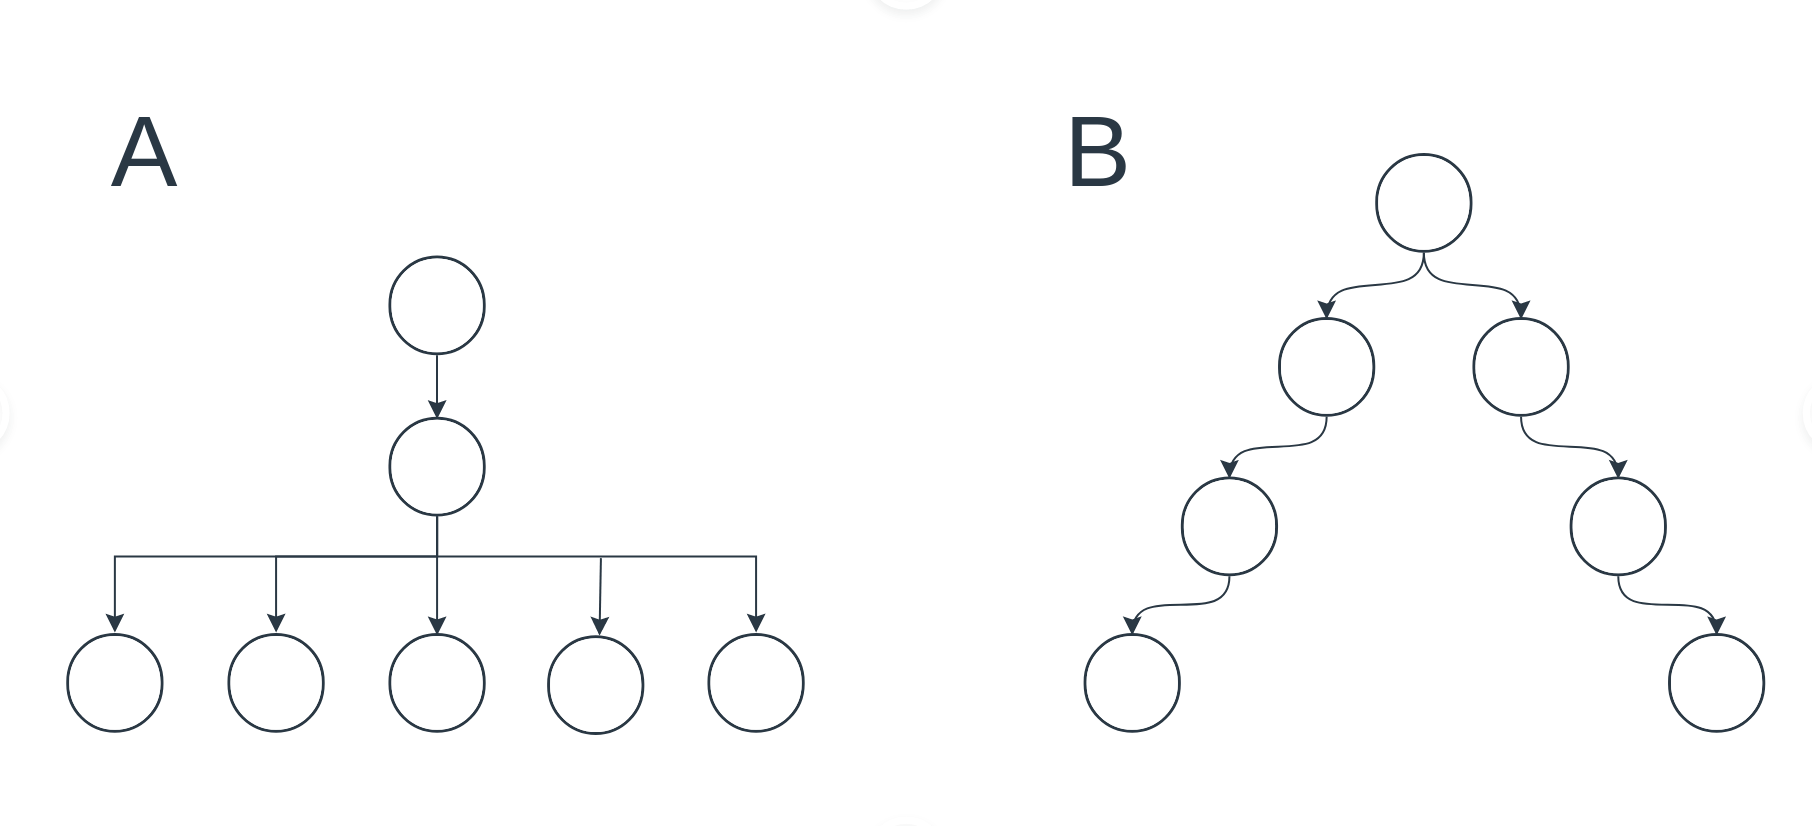
\includegraphics{conceptual_fig.png}
\caption{Example of populations with different levels of phenotypic and phylogenetic diveristy}
\end{figure}

\hypertarget{research-questions}{%
\subsection{Research questions}\label{research-questions}}

\begin{enumerate}
\def\labelenumi{\arabic{enumi}.}
\tightlist
\item
  Is phylogenetic diversity meaningfully different from phenotypic diversity in the context of evolutionary computation?
\end{enumerate}

The answer to this question is important. Intuitively, we might think that since these are both types of diversity, they should correlate pretty closely. Given that phylogenetic diversity is more computationally intensive to measure, if we're going to argue that it's something evolutionary computation researchers should pay attention to (spoilers: we are!), we need to show that it is meaningfully different.

\begin{enumerate}
\def\labelenumi{\arabic{enumi}.}
\setcounter{enumi}{1}
\tightlist
\item
  Is phylogenetic diversity more informative about outcomes in evolutionary computation than phenotypic diversity?
\end{enumerate}

The importance of this question is more obvious. We know that diversity is centrally linked to the success of evolutionary algorithms. There are hints scattered across the literature that certain types of diversity are more ``useful'' to solving problems than others. So our goal is for this work to move us towards a better understanding of which types of diversity we should be promoting in evolutionary algorithms.

\hypertarget{study-design}{%
\subsection{Study design}\label{study-design}}

We ran 5 selection schemes (random, tournament, fitness sharing, lexicase selection, and eco-ea) on 5 different problems (one designed to be a clean test environment, and 4 chosen to evoke the messy realities of real problems) and gathered a ludicrous amount of data. Here and in the paper, we attempt to focus very closely on getting answers to the two specific questions that we asked above (to avoid overwhelming ourselves or the reader with a firehose of data). There are many intriguing aspects of this data set that raise further questions, which we look forward to addressing in the future.

\hypertarget{results}{%
\subsection{Results}\label{results}}

\begin{enumerate}
\def\labelenumi{\arabic{enumi}.}
\item
  Phylogenetic diversity and phenotypic diversity behave differently to an extent that was even surprising to us.
\item
  Phylogenetic diversity is more predictive of success than phenotypic diversity in the vast majority of cases. The differences are often substantial (check out our effect sizes!).
\end{enumerate}

\hypertarget{caveatsareas-for-future-research}{%
\subsection{Caveats/areas for future research}\label{caveatsareas-for-future-research}}

\begin{itemize}
\item
  Phylogenetic diversity and phenotypic diversity are both broad classes of metrics, and there is substantial variation in how different phylogenetic diversity metrics behave in different contexts.
\item
  There is clearly variation in all of this over time and by fitness landscape.
\end{itemize}

\hypertarget{reproducing-our-work}{%
\section{Reproducing our work}\label{reproducing-our-work}}

\hypertarget{data-availability}{%
\subsection{Data availability}\label{data-availability}}

All data used in the paper is available via the \href{https://osf.io/6rndg/}{Open Science Framework}.

\hypertarget{code-availability}{%
\subsection{Code availability}\label{code-availability}}

All code used in the paper is available on \href{https://github.com/emilydolson/phylodiversity-metrics-in-EC-GPTP-2021/}{github}.

\hypertarget{dependencies}{%
\subsection{Dependencies}\label{dependencies}}

The C++ code to run these experiments requires:
- \href{https://github.com/devosoft/Empirical}{Empirical}
- The \href{https://github.com/emilydolson/ec_ecology_toolbox}{EC Ecology toolbox}

\hypertarget{compilation}{%
\subsection{Compilation}\label{compilation}}

You can compile and run the code used in the paper as follows:

\begin{Shaded}
\begin{Highlighting}[]
\CommentTok{# Clone Empirical}
\FunctionTok{git}\NormalTok{ clone --recursive https://github.com/devosoft/Empirical.git }

\CommentTok{# Clone EC-ecology-toolbox}
\FunctionTok{git}\NormalTok{ clone https://github.com/emilydolson/ec_ecology_toolbox.git}

\CommentTok{# Clone the repo for this project}
\FunctionTok{git}\NormalTok{ clone --recursive https://github.com/emilydolson/phylodiversity-metrics-in-EC-GPTP-2021.git}

\CommentTok{### Complex fitness landscapes}

\CommentTok{# Compile the executable to run experiments for this project}
\FunctionTok{make}

\CommentTok{# Run an experiment. To set parameters, use command line flags}
\CommentTok{# e.g. to set the selection scheme, run ./ecology_parameter_sweep -SELECTION 2}
\CommentTok{# To see all options, run ./ecology_parameter_sweep --help}
\ExtensionTok{./ecology_parameter_sweep}

\CommentTok{### Exploration diagnostic}

\CommentTok{# all of the code for the exploration diagnostic lives in the exploration_diagnostic submodule}
\BuiltInTok{cd}\NormalTok{ exploration_diagnostic}
\FunctionTok{make}
\ExtensionTok{./dia_world}

\CommentTok{# the dia_world executable can be configured in the same way as the ecology_parameter_sweep executable}
\end{Highlighting}
\end{Shaded}

\hypertarget{exploration-diagnostic}{%
\chapter{Exploration Diagnostic}\label{exploration-diagnostic}}

\hypertarget{setup}{%
\section{Setup}\label{setup}}

First, we need to do some set up to analyze our data

Include dependencies

\begin{Shaded}
\begin{Highlighting}[]
\KeywordTok{library}\NormalTok{(ggplot2)       }\CommentTok{# For plotting}
\KeywordTok{library}\NormalTok{(tidyverse)     }\CommentTok{# For data wrangling}
\KeywordTok{library}\NormalTok{(knitr)         }\CommentTok{# For making nice rmarkdown documents}
\KeywordTok{library}\NormalTok{(cowplot)       }\CommentTok{# For theme}
\KeywordTok{library}\NormalTok{(viridis)       }\CommentTok{# For color scale}
\KeywordTok{library}\NormalTok{(RColorBrewer)  }\CommentTok{# For more color scales}
\KeywordTok{library}\NormalTok{(rstatix)}
\KeywordTok{library}\NormalTok{(ggsignif)      }\CommentTok{# For adding pairwise significance to plots}
\KeywordTok{library}\NormalTok{(Hmisc)         }\CommentTok{# For bootstrapping condifence internvals}
\KeywordTok{library}\NormalTok{(kableExtra)    }\CommentTok{# For displaying nice tables}
\KeywordTok{source}\NormalTok{(}\StringTok{"https://gist.githubusercontent.com/benmarwick/2a1bb0133ff568cbe28d/raw/fb53bd97121f7f9ce947837ef1a4c65a73bffb3f/geom_flat_violin.R"}\NormalTok{) }\CommentTok{# For raincloud plots}
\KeywordTok{library}\NormalTok{(readr)        }\CommentTok{# For reading in data}
\KeywordTok{library}\NormalTok{(stringr)      }\CommentTok{# For manipulating string data}
\KeywordTok{library}\NormalTok{(ggpubr)       }\CommentTok{# For displaying correlation statistics on plots}
\KeywordTok{library}\NormalTok{(infotheo)     }\CommentTok{# For causality analysis}
\KeywordTok{library}\NormalTok{(scales)       }\CommentTok{# For displaying scales nicely in facetted plots}
\KeywordTok{library}\NormalTok{(osfr)         }\CommentTok{# For downloading the data for this project}
\end{Highlighting}
\end{Shaded}

These analyses were conducted in the following computing environment:

\begin{Shaded}
\begin{Highlighting}[]
\KeywordTok{print}\NormalTok{(version)}
\end{Highlighting}
\end{Shaded}

\begin{verbatim}
##                _                           
## platform       x86_64-pc-linux-gnu         
## arch           x86_64                      
## os             linux-gnu                   
## system         x86_64, linux-gnu           
## status                                     
## major          4                           
## minor          0.4                         
## year           2021                        
## month          02                          
## day            15                          
## svn rev        80002                       
## language       R                           
## version.string R version 4.0.4 (2021-02-15)
## nickname       Lost Library Book
\end{verbatim}

Setup constants to be used across plots

\begin{Shaded}
\begin{Highlighting}[]
\CommentTok{# Labeler for stats annotations}
\NormalTok{p_label <-}\StringTok{ }\ControlFlowTok{function}\NormalTok{(p_value) \{}
\NormalTok{  threshold =}\StringTok{ }\FloatTok{0.0001}
  \ControlFlowTok{if}\NormalTok{ (p_value }\OperatorTok{<}\StringTok{ }\NormalTok{threshold) \{}
    \KeywordTok{return}\NormalTok{(}\KeywordTok{paste0}\NormalTok{(}\StringTok{"p < "}\NormalTok{, threshold))}
\NormalTok{  \} }\ControlFlowTok{else}\NormalTok{ \{}
    \KeywordTok{return}\NormalTok{(}\KeywordTok{paste0}\NormalTok{(}\StringTok{"p = "}\NormalTok{, p_value))}
\NormalTok{  \}}
\NormalTok{\}}

\CommentTok{# Significance threshold}
\NormalTok{alpha <-}\StringTok{ }\FloatTok{0.05}

\CommentTok{# Common graph variables}
\NormalTok{performance_ylim <-}\StringTok{ }\DecValTok{1}
\NormalTok{coverage_ylim <-}\StringTok{ }\FloatTok{1.0}

\CommentTok{####### misc #######}
\CommentTok{# Configure our default graphing theme}
\KeywordTok{theme_set}\NormalTok{(}\KeywordTok{theme_cowplot}\NormalTok{())}
\end{Highlighting}
\end{Shaded}

The data for this project are hosted on \href{https://osf.io/6rndg/}{osf.io}. The following chunk downloads them automatically if they haven't already been downloaded.

\begin{Shaded}
\begin{Highlighting}[]
\CommentTok{# Read in data}
\KeywordTok{osf_retrieve_file}\NormalTok{(}\StringTok{"esm4r"}\NormalTok{) }\OperatorTok\StringTok{ }\KeywordTok{osf_download}\NormalTok{(}\DataTypeTok{conflicts =} \StringTok{"skip"}\NormalTok{)  }\CommentTok{# Download data from osf}
\NormalTok{data_loc <-}\StringTok{ "final_exploration_diagnostic_data.csv"}

\NormalTok{data <-}\StringTok{ }\KeywordTok{read_csv}\NormalTok{(data_loc, }\DataTypeTok{na=}\KeywordTok{c}\NormalTok{(}\StringTok{"NONE"}\NormalTok{, }\StringTok{"NA"}\NormalTok{, }\StringTok{""}\NormalTok{))}

\CommentTok{## Clean up data columns}

\CommentTok{# Make selection name column human readable}
\NormalTok{data <-}\StringTok{ }\NormalTok{data }\OperatorTok\StringTok{ }\KeywordTok{mutate}\NormalTok{(}\DataTypeTok{selection_name =} \KeywordTok{as.factor}\NormalTok{(}\KeywordTok{case_when}\NormalTok{(}
\NormalTok{  selection_name }\OperatorTok{==}\StringTok{ "EpsilonLexicase"} \OperatorTok{~}\StringTok{ "Lexicase"}\NormalTok{,}
\NormalTok{  TOUR_SIZE }\OperatorTok{==}\StringTok{ }\DecValTok{1} \OperatorTok{~}\StringTok{ "Random"}\NormalTok{,}
\NormalTok{  selection_name }\OperatorTok{==}\StringTok{ "Tournament"} \OperatorTok{~}\StringTok{ "Tournament"}\NormalTok{,}
\NormalTok{  selection_name }\OperatorTok{==}\StringTok{ "FitnessSharing"} \OperatorTok{~}\StringTok{ "Fitness Sharing"}\NormalTok{,}
\NormalTok{  selection_name }\OperatorTok{==}\StringTok{ "EcoEa"} \OperatorTok{~}\StringTok{ "EcoEA"}
\NormalTok{)))}

\CommentTok{# Calculate performance statistics.}
\CommentTok{# Elite trait avg is the avg per-site performance of the best individual}
\NormalTok{data}\OperatorTok{$}\NormalTok{elite_trait_avg <-}
\StringTok{  }\NormalTok{data}\OperatorTok{$}\NormalTok{ele_agg_per }\OperatorTok{/}\StringTok{ }\NormalTok{data}\OperatorTok{$}\NormalTok{OBJECTIVE_CNT}
\NormalTok{data}\OperatorTok{$}\NormalTok{unique_start_positions_coverage <-}
\StringTok{  }\NormalTok{data}\OperatorTok{$}\NormalTok{uni_str_pos }\OperatorTok{/}\StringTok{ }\NormalTok{data}\OperatorTok{$}\NormalTok{OBJECTIVE_CNT}

\CommentTok{# Convert elite_trait_avg to percent of maximum possible}
\NormalTok{data}\OperatorTok{$}\NormalTok{elite_trait_avg <-}\StringTok{ }\NormalTok{data}\OperatorTok{$}\NormalTok{elite_trait_avg}\OperatorTok{/}\NormalTok{data}\OperatorTok{$}\NormalTok{TARGET}

\CommentTok{# Grab data from just the final time point}
\NormalTok{final_data <-}\StringTok{ }\KeywordTok{filter}\NormalTok{(data, evaluations}\OperatorTok{==}\KeywordTok{max}\NormalTok{(data}\OperatorTok{$}\NormalTok{evaluations))}
\end{Highlighting}
\end{Shaded}

\hypertarget{performance}{%
\section{Performance}\label{performance}}

For context, it's important to know how each selection scheme performed on the exploration diagnostic.

\hypertarget{over-time}{%
\subsection{Over time}\label{over-time}}

First we look at the dynamics of performance over time.

\hypertarget{trait-performance}{%
\subsubsection{Trait performance}\label{trait-performance}}

Here, we plot average trait performance (i.e.~fitness) over time for each selection scheme. We log the x-axis because Eco-EA gains fitness over a very long time scale, whereas the interesting dynamics for the other selection schemes occur relatively quickly.

\begin{Shaded}
\begin{Highlighting}[]
\KeywordTok{ggplot}\NormalTok{(}
\NormalTok{    data,}
    \KeywordTok{aes}\NormalTok{(}
      \DataTypeTok{x=}\NormalTok{gen,                 }\CommentTok{# Generations}
      \DataTypeTok{y=}\NormalTok{elite_trait_avg,     }\CommentTok{# Performance}
      \DataTypeTok{color=}\NormalTok{selection_name,  }\CommentTok{# Selection scheme}
      \DataTypeTok{fill=}\NormalTok{selection_name}
\NormalTok{    )}
\NormalTok{  ) }\OperatorTok{+}
\StringTok{  }\KeywordTok{stat_summary}\NormalTok{(}\DataTypeTok{geom=}\StringTok{"line"}\NormalTok{, }\DataTypeTok{fun=}\NormalTok{mean) }\OperatorTok{+}\StringTok{ }\CommentTok{# Plot line showing mean for each selection scheme}
\StringTok{  }\KeywordTok{stat_summary}\NormalTok{(  }\CommentTok{# Add shading around each line indicating 95% confiedence interval}
    \DataTypeTok{geom=}\StringTok{"ribbon"}\NormalTok{,}
    \DataTypeTok{fun.data=}\StringTok{"mean_cl_boot"}\NormalTok{,}
    \DataTypeTok{fun.args=}\KeywordTok{list}\NormalTok{(}\DataTypeTok{conf.int=}\FloatTok{0.95}\NormalTok{),}
    \DataTypeTok{alpha=}\FloatTok{0.2}\NormalTok{,}
    \DataTypeTok{linetype=}\DecValTok{0}
\NormalTok{  ) }\OperatorTok{+}
\StringTok{  }\KeywordTok{scale_y_continuous}\NormalTok{(}
    \DataTypeTok{name=}\StringTok{"Average trait performance"}\NormalTok{, }\CommentTok{# Set y axis title}
    \DataTypeTok{limits=}\KeywordTok{c}\NormalTok{(}\DecValTok{0}\NormalTok{, performance_ylim)  }\CommentTok{# Set y axis range to include all possible performance values}
\NormalTok{  ) }\OperatorTok{+}
\StringTok{  }\KeywordTok{scale_x_log10}\NormalTok{(  }\CommentTok{# Log x axis}
    \DataTypeTok{name=}\StringTok{"Generation"} \CommentTok{# Set x axis title}
\NormalTok{  ) }\OperatorTok{+}
\StringTok{  }\KeywordTok{scale_color_discrete}\NormalTok{(}\StringTok{"Selection"}\NormalTok{) }\OperatorTok{+}\StringTok{ }\CommentTok{# Set legend title}
\StringTok{  }\KeywordTok{scale_fill_discrete}\NormalTok{(}\StringTok{"Selection"}\NormalTok{)    }\CommentTok{# Set legend title}
\end{Highlighting}
\end{Shaded}

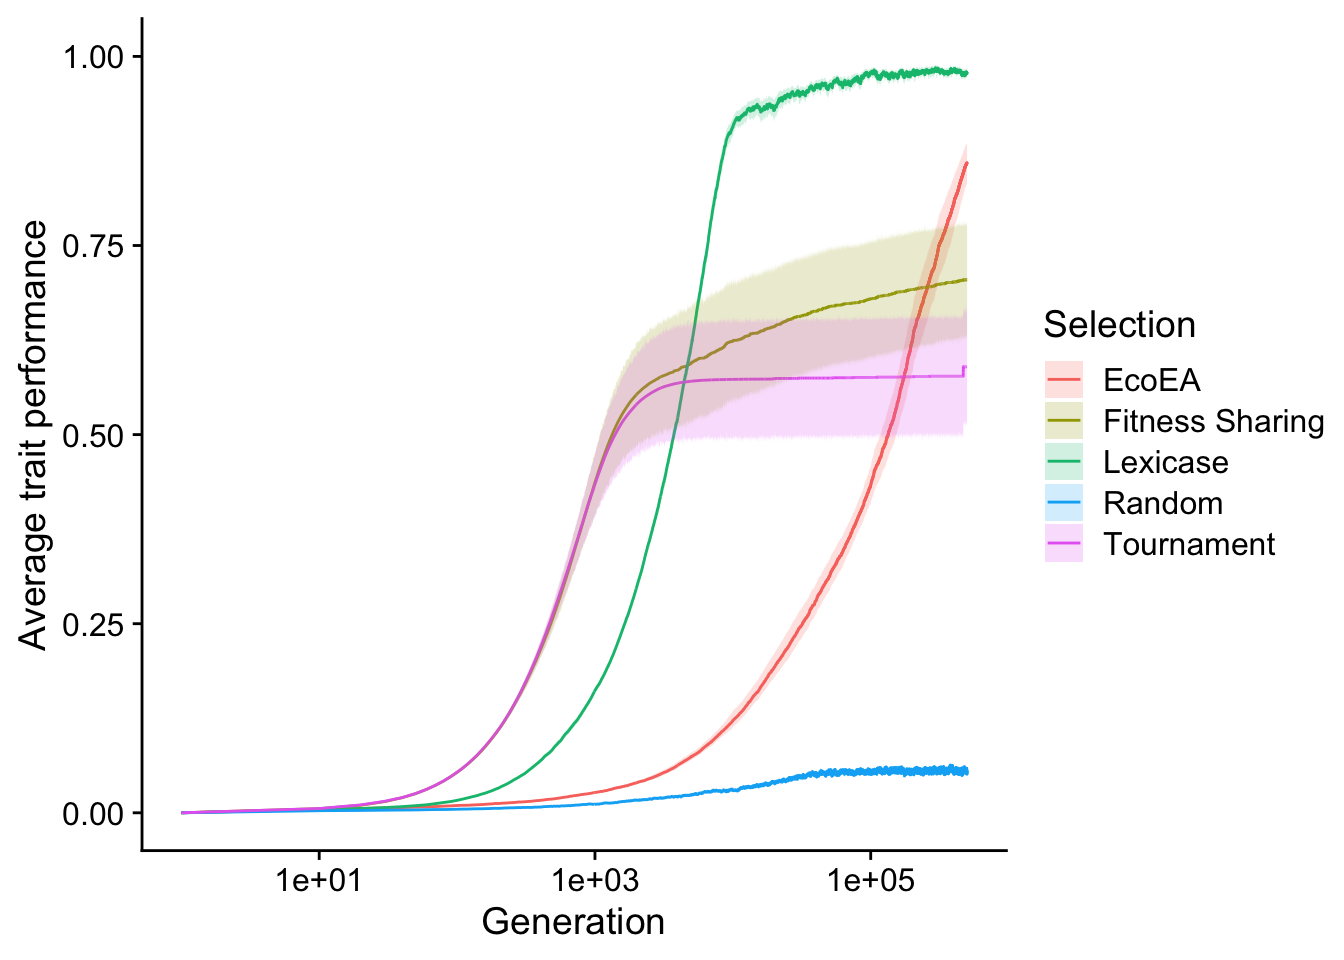
\includegraphics{phylodiversity-in-EC-supplement_files/figure-latex/performance_over_time-1.pdf}

As observed by Hernandez et al.~in their original paper on the exploration diagnostic \citep{hernandez_ExplorationExplorationMeasuring_2021}, fitness in tournament selection initially increases quickly and then plateaus. Fitness in lexicase selection increases slightly slower but plateaus at a much higher value (nearly 100\%). Fitness sharing behaves similarly to tournament selection, but maintains a slight upward trajectory (note that, because the x axis is on a log scale, this trajectory is very gradual). Eco-EA takes substantially longer to increase in fitness but ultimately surpasses fitness sharing and tournament selection. It is unclear whether it would pass lexicase selection if these runs were allowed to continue for slightly longer; they do not appear to have plateaued yet. We chose to cut them off at 500,000 generations due to resource constraints and the fact that the questions we're asking here are not really about final fitness.

\hypertarget{activation-position-coverage}{%
\subsubsection{Activation position coverage}\label{activation-position-coverage}}

Out of curiosity, we also ran the analysis of unique activation positions present in the population, used by Hernandez et. al.~This analysis tells us about the diversity of start positions for the coding region represented in the population. As the set of start positions in the population tends to represent a meaningful constraint on the number of paths through the fitness landscape that are currently accessible, this is in some sense a metric of useful diversity in the population

\begin{Shaded}
\begin{Highlighting}[]
\KeywordTok{ggplot}\NormalTok{(data, }\KeywordTok{aes}\NormalTok{(}\DataTypeTok{x=}\NormalTok{gen, }\DataTypeTok{y=}\NormalTok{unique_start_positions_coverage, }\DataTypeTok{color=}\NormalTok{selection_name, }\DataTypeTok{fill=}\NormalTok{selection_name)) }\OperatorTok{+}
\StringTok{  }\KeywordTok{stat_summary}\NormalTok{(}\DataTypeTok{geom=}\StringTok{"line"}\NormalTok{, }\DataTypeTok{fun=}\NormalTok{mean) }\OperatorTok{+}
\StringTok{  }\KeywordTok{stat_summary}\NormalTok{(}
    \DataTypeTok{geom=}\StringTok{"ribbon"}\NormalTok{,}
    \DataTypeTok{fun.data=}\StringTok{"mean_cl_boot"}\NormalTok{,}
    \DataTypeTok{fun.args=}\KeywordTok{list}\NormalTok{(}\DataTypeTok{conf.int=}\FloatTok{0.95}\NormalTok{),}
    \DataTypeTok{alpha=}\FloatTok{0.2}\NormalTok{,}
    \DataTypeTok{linetype=}\DecValTok{0}
\NormalTok{  ) }\OperatorTok{+}
\StringTok{  }\KeywordTok{scale_y_continuous}\NormalTok{(}
    \DataTypeTok{name=}\StringTok{"Activation position coverage"}
\NormalTok{  ) }\OperatorTok{+}
\StringTok{  }\KeywordTok{scale_x_log10}\NormalTok{(}
    \DataTypeTok{name=}\StringTok{"Generation"}
\NormalTok{  ) }\OperatorTok{+}
\StringTok{  }\KeywordTok{scale_color_discrete}\NormalTok{(}\StringTok{"Selection"}\NormalTok{)}\OperatorTok{+}
\StringTok{  }\KeywordTok{scale_fill_discrete}\NormalTok{(}\StringTok{"Selection"}\NormalTok{)}
\end{Highlighting}
\end{Shaded}

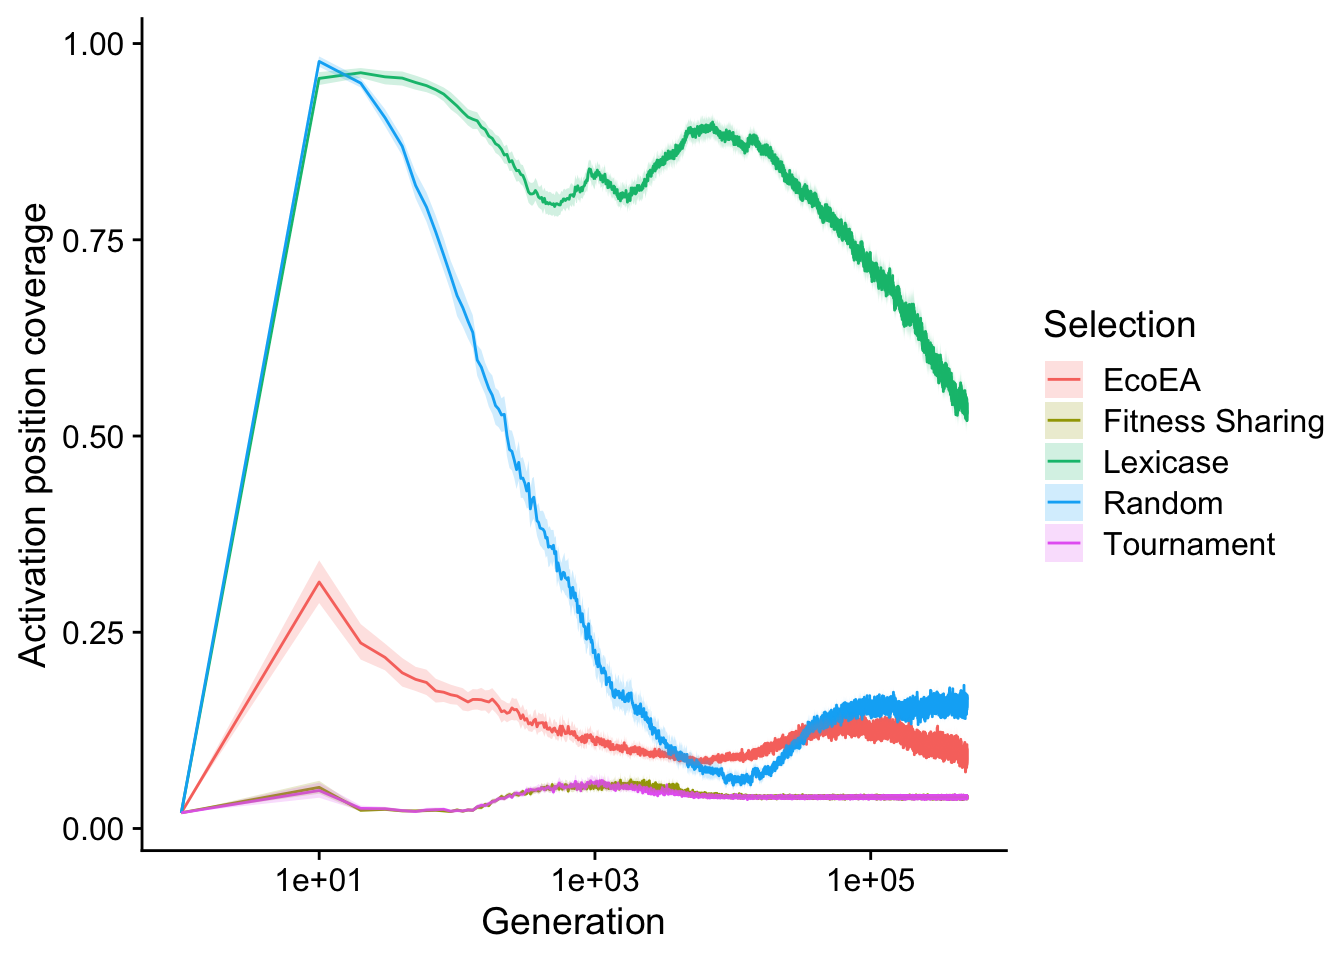
\includegraphics{phylodiversity-in-EC-supplement_files/figure-latex/unique_start_positions-1.pdf}

We see that lexicase selection maintains by far that largest number of unique start positions, even surpassing the number maintained by random drift. This suggests that lexicase selection is actively selecting for maintaining a diversity of start positions. Tournament selection and fitness sharing perform virtually identically, with Eco-EA falling in between.

\hypertarget{final}{%
\subsection{Final}\label{final}}

While trends over time are more informative, it can be hard to visualize the full distribution (particularly the extent of variation). Thus, we also conduct a more detailed analysis of performance at the final time point.

\hypertarget{trait-performance-1}{%
\subsubsection{Trait performance}\label{trait-performance-1}}

First we conduct statistics to identify which selection schemes are significantly different from each other.

\begin{Shaded}
\begin{Highlighting}[]
\CommentTok{# Compute manual labels for geom_signif}
\NormalTok{stat.test <-}\StringTok{ }\NormalTok{final_data }\OperatorTok
\StringTok{  }\KeywordTok{wilcox_test}\NormalTok{(elite_trait_avg }\OperatorTok{~}\StringTok{ }\NormalTok{selection_name) }\OperatorTok
\StringTok{  }\KeywordTok{adjust_pvalue}\NormalTok{(}\DataTypeTok{method =} \StringTok{"bonferroni"}\NormalTok{) }\OperatorTok\StringTok{  }\CommentTok{# Apply Bonferroni correction for multiple comparisons}
\StringTok{  }\KeywordTok{add_significance}\NormalTok{() }\OperatorTok
\StringTok{  }\KeywordTok{add_xy_position}\NormalTok{(}\DataTypeTok{x=}\StringTok{"selection_name"}\NormalTok{,}\DataTypeTok{step.increase=}\DecValTok{1}\NormalTok{)}
\NormalTok{stat.test}\OperatorTok{$}\NormalTok{label <-}\StringTok{ }\KeywordTok{mapply}\NormalTok{(p_label,stat.test}\OperatorTok{$}\NormalTok{p.adj)}
\end{Highlighting}
\end{Shaded}

Then we make raincloud plots \citep{allen_RaincloudPlotsMultiplatform_2021a} of each selection scheme.

\begin{Shaded}
\begin{Highlighting}[]
\NormalTok{elite_final_performance_fig <-}\StringTok{ }\KeywordTok{ggplot}\NormalTok{(}
\NormalTok{    final_data,}
    \KeywordTok{aes}\NormalTok{(}
      \DataTypeTok{x=}\NormalTok{selection_name,}
      \DataTypeTok{y=}\NormalTok{elite_trait_avg,}
      \DataTypeTok{fill=}\NormalTok{selection_name}
\NormalTok{    )}
\NormalTok{  ) }\OperatorTok{+}
\StringTok{  }\KeywordTok{geom_flat_violin}\NormalTok{(}
    \DataTypeTok{position =} \KeywordTok{position_nudge}\NormalTok{(}\DataTypeTok{x =} \FloatTok{.2}\NormalTok{, }\DataTypeTok{y =} \DecValTok{0}\NormalTok{),}
    \DataTypeTok{alpha =} \FloatTok{.8}\NormalTok{,}
    \DataTypeTok{scale=}\StringTok{"width"}
\NormalTok{  ) }\OperatorTok{+}
\StringTok{  }\KeywordTok{geom_point}\NormalTok{(}
    \DataTypeTok{mapping=}\KeywordTok{aes}\NormalTok{(}\DataTypeTok{color=}\NormalTok{selection_name),}
    \DataTypeTok{position =} \KeywordTok{position_jitter}\NormalTok{(}\DataTypeTok{width =} \FloatTok{.15}\NormalTok{),}
    \DataTypeTok{size =} \FloatTok{.5}\NormalTok{,}
    \DataTypeTok{alpha =} \FloatTok{0.8}
\NormalTok{  ) }\OperatorTok{+}
\StringTok{  }\KeywordTok{geom_boxplot}\NormalTok{(}
    \DataTypeTok{width =} \FloatTok{.1}\NormalTok{,}
    \DataTypeTok{outlier.shape =} \OtherTok{NA}\NormalTok{,}
    \DataTypeTok{alpha =} \FloatTok{0.5}
\NormalTok{  ) }\OperatorTok{+}
\StringTok{  }\KeywordTok{scale_y_continuous}\NormalTok{(}
    \DataTypeTok{name=}\StringTok{"Average trait performance"}\NormalTok{,}
    \DataTypeTok{limits=}\KeywordTok{c}\NormalTok{(}\DecValTok{0}\NormalTok{, performance_ylim)}
\NormalTok{  ) }\OperatorTok{+}
\StringTok{  }\KeywordTok{scale_x_discrete}\NormalTok{(}
    \DataTypeTok{name=}\StringTok{"Selection"}
\NormalTok{  ) }\OperatorTok{+}
\StringTok{  }\KeywordTok{scale_fill_discrete}\NormalTok{(}
    \DataTypeTok{name=}\StringTok{"Selection"}
\NormalTok{  ) }\OperatorTok{+}
\StringTok{  }\KeywordTok{scale_color_discrete}\NormalTok{(}
    \DataTypeTok{name=}\StringTok{"Selection"}
\NormalTok{  ) }\OperatorTok{+}\StringTok{ }
\StringTok{  }\KeywordTok{theme}\NormalTok{(}\DataTypeTok{legend.position=}\StringTok{"none"}\NormalTok{)}
\NormalTok{elite_final_performance_fig}
\end{Highlighting}
\end{Shaded}

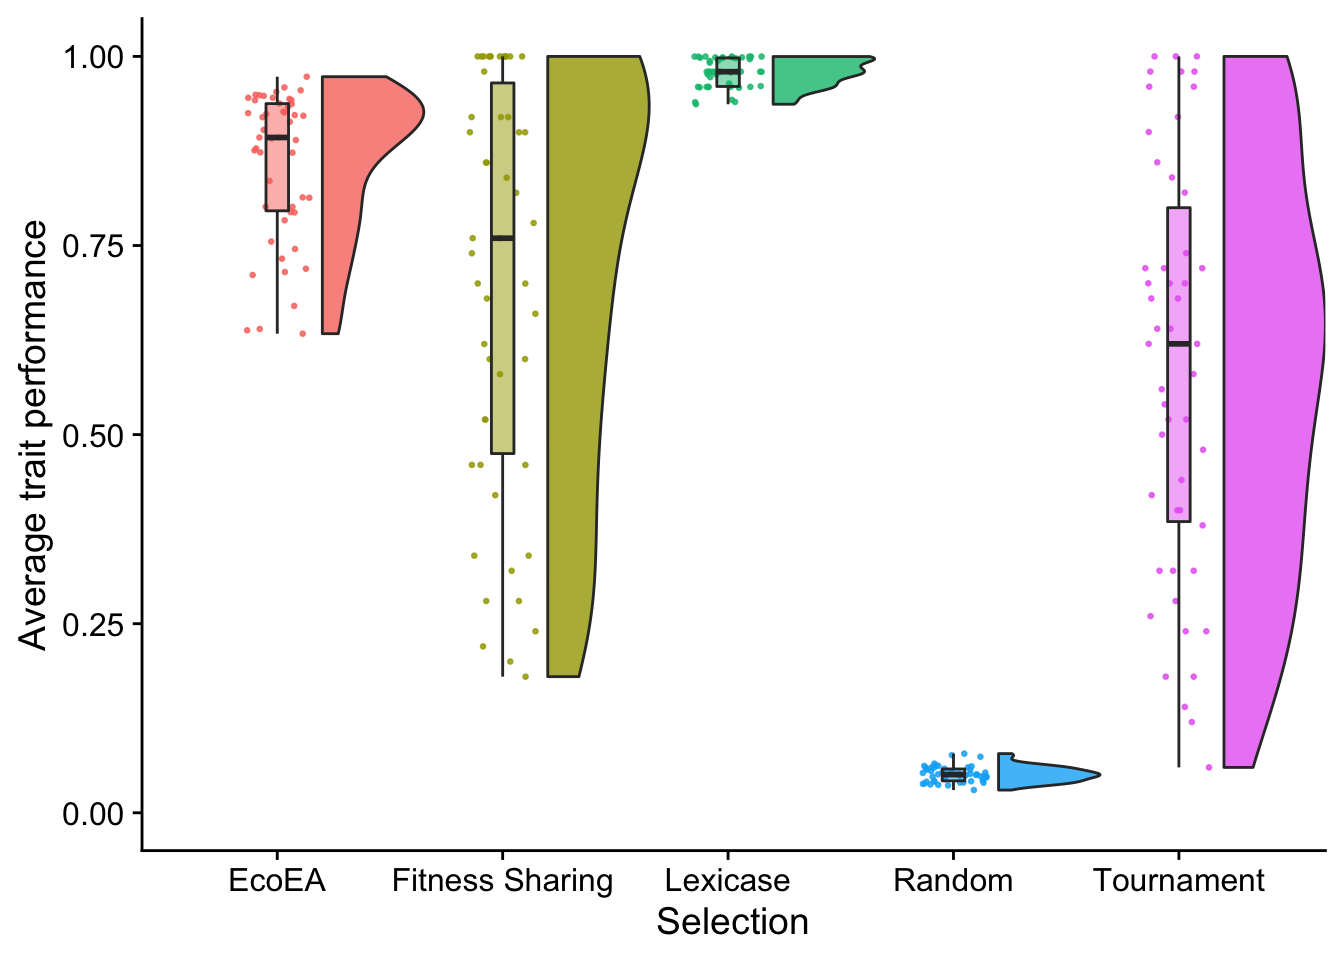
\includegraphics{phylodiversity-in-EC-supplement_files/figure-latex/final_performance_plot-1.pdf}

These observations look fairly consistent with the timeseries plots.

Next, we output the results of our significance testing.

\begin{Shaded}
\begin{Highlighting}[]
\NormalTok{stat.test }\OperatorTok
\StringTok{  }\KeywordTok{kbl}\NormalTok{() }\OperatorTok
\StringTok{  }\KeywordTok{kable_styling}\NormalTok{(}
    \DataTypeTok{bootstrap_options =} \KeywordTok{c}\NormalTok{(}
      \StringTok{"striped"}\NormalTok{,}
      \StringTok{"hover"}\NormalTok{,}
      \StringTok{"condensed"}\NormalTok{,}
      \StringTok{"responsive"}
\NormalTok{    )}
\NormalTok{  ) }\OperatorTok
\StringTok{  }\KeywordTok{scroll_box}\NormalTok{(}\DataTypeTok{width=}\StringTok{"600px"}\NormalTok{)}
\end{Highlighting}
\end{Shaded}

\begin{table}
\centering
\begin{tabular}[t]{l|l|l|r|r|r|r|r|l|r|l|r|r|l}
\hline
.y. & group1 & group2 & n1 & n2 & statistic & p & p.adj & p.adj.signif & y.position & groups & xmin & xmax & label\\
\hline
elite\_trait\_avg & EcoEA & Fitness Sharing & 50 & 50 & 1561 & 3.20e-02 & 3.20e-01 & ns & 1.922000 & EcoEA          , Fitness Sharing & 1 & 2 & p = 0.32\\
\hline
elite\_trait\_avg & EcoEA & Lexicase & 50 & 47 & 60 & 0.00e+00 & 0.00e+00 & **** & 2.946444 & EcoEA   , Lexicase & 1 & 3 & p < 1e-04\\
\hline
elite\_trait\_avg & EcoEA & Random & 50 & 50 & 2500 & 0.00e+00 & 0.00e+00 & **** & 3.970889 & EcoEA , Random & 1 & 4 & p < 1e-04\\
\hline
elite\_trait\_avg & EcoEA & Tournament & 50 & 50 & 1939 & 2.10e-06 & 2.07e-05 & **** & 4.995333 & EcoEA     , Tournament & 1 & 5 & p < 1e-04\\
\hline
elite\_trait\_avg & Fitness Sharing & Lexicase & 50 & 47 & 593 & 2.69e-05 & 2.69e-04 & *** & 6.019778 & Fitness Sharing, Lexicase & 2 & 3 & p = 0.000269\\
\hline
elite\_trait\_avg & Fitness Sharing & Random & 50 & 50 & 2500 & 0.00e+00 & 0.00e+00 & **** & 7.044222 & Fitness Sharing, Random & 2 & 4 & p < 1e-04\\
\hline
elite\_trait\_avg & Fitness Sharing & Tournament & 50 & 50 & 1549 & 4.00e-02 & 4.00e-01 & ns & 8.068667 & Fitness Sharing, Tournament & 2 & 5 & p = 0.4\\
\hline
elite\_trait\_avg & Lexicase & Random & 47 & 50 & 2350 & 0.00e+00 & 0.00e+00 & **** & 9.093111 & Lexicase, Random & 3 & 4 & p < 1e-04\\
\hline
elite\_trait\_avg & Lexicase & Tournament & 47 & 50 & 2098 & 0.00e+00 & 0.00e+00 & **** & 10.117556 & Lexicase  , Tournament & 3 & 5 & p < 1e-04\\
\hline
elite\_trait\_avg & Random & Tournament & 50 & 50 & 10 & 0.00e+00 & 0.00e+00 & **** & 11.142000 & Random    , Tournament & 4 & 5 & p < 1e-04\\
\hline
\end{tabular}
\end{table}

Fitness sharing did not perform significantly differently from Eco-EA or Tournament selection, but all other selection schemes are significantly different.

\hypertarget{final-activation-position-coverage}{%
\subsubsection{Final activation position Coverage}\label{final-activation-position-coverage}}

Now we do the same analysis for final activation position coverage.

First we calculate the statistics

\begin{Shaded}
\begin{Highlighting}[]
\CommentTok{# Compute manual labels for geom_signif}
\NormalTok{stat.test <-}\StringTok{ }\NormalTok{final_data }\OperatorTok
\StringTok{  }\KeywordTok{wilcox_test}\NormalTok{(unique_start_positions_coverage }\OperatorTok{~}\StringTok{ }\NormalTok{selection_name) }\OperatorTok
\StringTok{  }\KeywordTok{adjust_pvalue}\NormalTok{(}\DataTypeTok{method =} \StringTok{"bonferroni"}\NormalTok{) }\OperatorTok
\StringTok{  }\KeywordTok{add_significance}\NormalTok{() }\OperatorTok
\StringTok{  }\KeywordTok{add_xy_position}\NormalTok{(}\DataTypeTok{x=}\StringTok{"selection_name"}\NormalTok{,}\DataTypeTok{step.increase=}\DecValTok{1}\NormalTok{)}
\NormalTok{stat.test}\OperatorTok{$}\NormalTok{manual_position <-}\StringTok{ }\NormalTok{stat.test}\OperatorTok{$}\NormalTok{y.position }\OperatorTok{*}\StringTok{ }\FloatTok{1.05}
\NormalTok{stat.test}\OperatorTok{$}\NormalTok{label <-}\StringTok{ }\KeywordTok{mapply}\NormalTok{(p_label,stat.test}\OperatorTok{$}\NormalTok{p.adj)}
\end{Highlighting}
\end{Shaded}

Then we make raincloud plots

\begin{Shaded}
\begin{Highlighting}[]
\NormalTok{unique_start_positions_coverage_final_fig <-}\StringTok{ }\KeywordTok{ggplot}\NormalTok{(}
\NormalTok{    final_data,}
    \KeywordTok{aes}\NormalTok{(}
      \DataTypeTok{x=}\NormalTok{selection_name,}
      \DataTypeTok{y=}\NormalTok{unique_start_positions_coverage,}
      \DataTypeTok{fill=}\NormalTok{selection_name}
\NormalTok{    )}
\NormalTok{  ) }\OperatorTok{+}
\StringTok{  }\KeywordTok{geom_flat_violin}\NormalTok{(}
    \DataTypeTok{position =} \KeywordTok{position_nudge}\NormalTok{(}\DataTypeTok{x =} \FloatTok{.2}\NormalTok{, }\DataTypeTok{y =} \DecValTok{0}\NormalTok{),}
    \DataTypeTok{alpha =} \FloatTok{.8}\NormalTok{,}
    \DataTypeTok{scale=}\StringTok{"width"}
\NormalTok{  ) }\OperatorTok{+}
\StringTok{  }\KeywordTok{geom_point}\NormalTok{(}
    \DataTypeTok{mapping=}\KeywordTok{aes}\NormalTok{(}\DataTypeTok{color=}\NormalTok{selection_name),}
    \DataTypeTok{position =} \KeywordTok{position_jitter}\NormalTok{(}\DataTypeTok{width =} \FloatTok{.15}\NormalTok{),}
    \DataTypeTok{size =} \FloatTok{.5}\NormalTok{,}
    \DataTypeTok{alpha =} \FloatTok{0.8}
\NormalTok{  ) }\OperatorTok{+}
\StringTok{  }\KeywordTok{geom_boxplot}\NormalTok{(}
    \DataTypeTok{width =} \FloatTok{.1}\NormalTok{,}
    \DataTypeTok{outlier.shape =} \OtherTok{NA}\NormalTok{,}
    \DataTypeTok{alpha =} \FloatTok{0.5}
\NormalTok{  ) }\OperatorTok{+}
\StringTok{  }\KeywordTok{scale_y_continuous}\NormalTok{(}
    \DataTypeTok{name=}\StringTok{"Activation position coverage"}\NormalTok{,}
    \DataTypeTok{limits=}\KeywordTok{c}\NormalTok{(}\DecValTok{0}\NormalTok{, coverage_ylim)}
\NormalTok{  ) }\OperatorTok{+}
\StringTok{  }\KeywordTok{scale_x_discrete}\NormalTok{(}
    \DataTypeTok{name=}\StringTok{"Selection"}
\NormalTok{  ) }\OperatorTok{+}
\StringTok{  }\KeywordTok{scale_fill_discrete}\NormalTok{(}
    \DataTypeTok{name=}\StringTok{"Selection"}
\NormalTok{  ) }\OperatorTok{+}
\StringTok{  }\KeywordTok{scale_color_discrete}\NormalTok{(}
    \DataTypeTok{name=}\StringTok{"Selection"}
\NormalTok{  ) }\OperatorTok{+}
\StringTok{  }\KeywordTok{theme}\NormalTok{(}
    \DataTypeTok{legend.position=}\StringTok{"none"}
\NormalTok{  )}
\NormalTok{unique_start_positions_coverage_final_fig}
\end{Highlighting}
\end{Shaded}

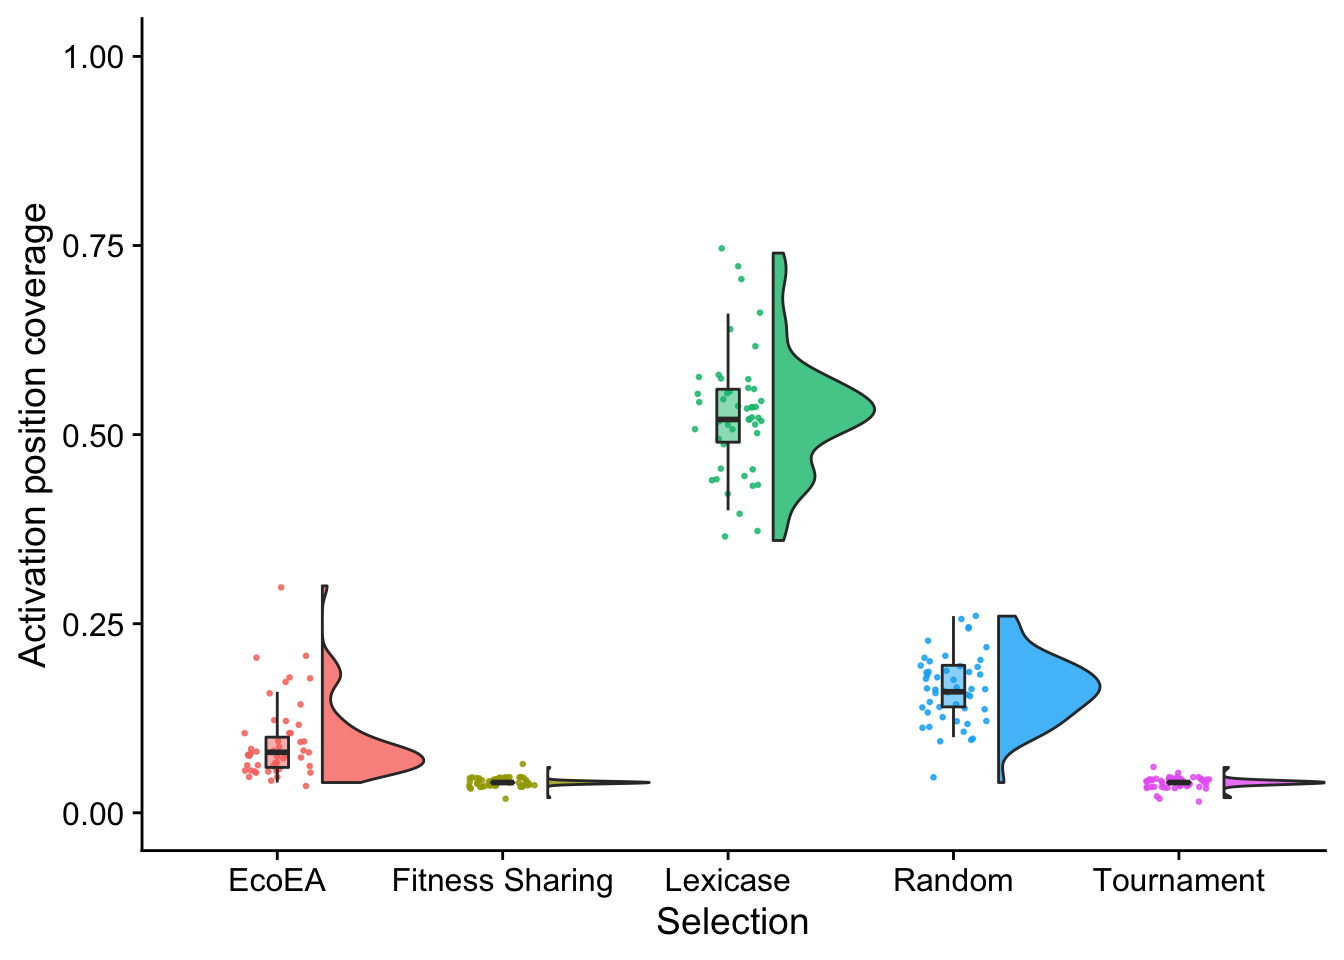
\includegraphics{phylodiversity-in-EC-supplement_files/figure-latex/unique_start_positions_final-1.pdf}

These also look unsurprising.

Lastly, we output the results of significance testing.

\begin{Shaded}
\begin{Highlighting}[]
\NormalTok{stat.test }\OperatorTok
\StringTok{  }\KeywordTok{kbl}\NormalTok{() }\OperatorTok
\StringTok{  }\KeywordTok{kable_styling}\NormalTok{(}
    \DataTypeTok{bootstrap_options =} \KeywordTok{c}\NormalTok{(}
      \StringTok{"striped"}\NormalTok{,}
      \StringTok{"hover"}\NormalTok{,}
      \StringTok{"condensed"}\NormalTok{,}
      \StringTok{"responsive"}
\NormalTok{    )}
\NormalTok{  ) }\OperatorTok
\StringTok{  }\KeywordTok{scroll_box}\NormalTok{(}\DataTypeTok{width=}\StringTok{"600px"}\NormalTok{)}
\end{Highlighting}
\end{Shaded}

\begin{table}
\centering
\begin{tabular}[t]{l|l|l|r|r|r|r|r|l|r|l|r|r|r|l}
\hline
.y. & group1 & group2 & n1 & n2 & statistic & p & p.adj & p.adj.signif & y.position & groups & xmin & xmax & manual\_position & label\\
\hline
unique\_start\_positions\_coverage & EcoEA & Fitness Sharing & 50 & 50 & 2392.5 & 0.000 & 0 & **** & 1.420000 & EcoEA          , Fitness Sharing & 1 & 2 & 1.491000 & p < 1e-04\\
\hline
unique\_start\_positions\_coverage & EcoEA & Lexicase & 50 & 47 & 0.0 & 0.000 & 0 & **** & 2.175556 & EcoEA   , Lexicase & 1 & 3 & 2.284333 & p < 1e-04\\
\hline
unique\_start\_positions\_coverage & EcoEA & Random & 50 & 50 & 339.0 & 0.000 & 0 & **** & 2.931111 & EcoEA , Random & 1 & 4 & 3.077667 & p < 1e-04\\
\hline
unique\_start\_positions\_coverage & EcoEA & Tournament & 50 & 50 & 2387.0 & 0.000 & 0 & **** & 3.686667 & EcoEA     , Tournament & 1 & 5 & 3.871000 & p < 1e-04\\
\hline
unique\_start\_positions\_coverage & Fitness Sharing & Lexicase & 50 & 47 & 0.0 & 0.000 & 0 & **** & 4.442222 & Fitness Sharing, Lexicase & 2 & 3 & 4.664333 & p < 1e-04\\
\hline
unique\_start\_positions\_coverage & Fitness Sharing & Random & 50 & 50 & 25.0 & 0.000 & 0 & **** & 5.197778 & Fitness Sharing, Random & 2 & 4 & 5.457667 & p < 1e-04\\
\hline
unique\_start\_positions\_coverage & Fitness Sharing & Tournament & 50 & 50 & 1274.5 & 0.708 & 1 & ns & 5.953333 & Fitness Sharing, Tournament & 2 & 5 & 6.251000 & p = 1\\
\hline
unique\_start\_positions\_coverage & Lexicase & Random & 47 & 50 & 2350.0 & 0.000 & 0 & **** & 6.708889 & Lexicase, Random & 3 & 4 & 7.044333 & p < 1e-04\\
\hline
unique\_start\_positions\_coverage & Lexicase & Tournament & 47 & 50 & 2350.0 & 0.000 & 0 & **** & 7.464444 & Lexicase  , Tournament & 3 & 5 & 7.837667 & p < 1e-04\\
\hline
unique\_start\_positions\_coverage & Random & Tournament & 50 & 50 & 2475.5 & 0.000 & 0 & **** & 8.220000 & Random    , Tournament & 4 & 5 & 8.631000 & p < 1e-04\\
\hline
\end{tabular}
\end{table}

\hypertarget{phylogenetic-diversity}{%
\section{Phylogenetic diversity}\label{phylogenetic-diversity}}

Next, we analyze the behavior of phylogenetic diversity on the exploration diagnostic.

\hypertarget{relationship-between-different-types-of-pylogenetic-diversity}{%
\subsection{Relationship between different types of pylogenetic diversity}\label{relationship-between-different-types-of-pylogenetic-diversity}}

First, to get a big-picture overview, we make correlation matrices of all the different phylogenetic diversity metrics:

\begin{Shaded}
\begin{Highlighting}[]
\NormalTok{final_data }\OperatorTok\StringTok{ }
\StringTok{  }\KeywordTok{transmute}\NormalTok{(}\DataTypeTok{MinPD=}\NormalTok{min_phenotype_pairwise_distance, }
            \DataTypeTok{MeanPD=}\NormalTok{mean_phenotype_pairwise_distance, }
            \DataTypeTok{MaxPD=}\NormalTok{max_phenotype_pairwise_distance, }
            \DataTypeTok{VarPD=}\NormalTok{variance_phenotype_pairwise_distance, }
            \DataTypeTok{MinED =}\NormalTok{ min_phenotype_evolutionary_distinctiveness,}
            \DataTypeTok{MeanED=}\NormalTok{ mean_phenotype_evolutionary_distinctiveness,}
            \DataTypeTok{MaxED=}\NormalTok{max_phenotype_evolutionary_distinctiveness,}
            \DataTypeTok{VarED=}\NormalTok{variance_phenotype_evolutionary_distinctiveness,}
            \DataTypeTok{PD=}\NormalTok{phenotype_current_phylogenetic_diversity,  }\CommentTok{# See Faith 1992}
            \DataTypeTok{MRCA=}\NormalTok{phen_mrca_depth,  }\CommentTok{# Phylogenetic depth of most recent common ancestor}
            \DataTypeTok{N=}\NormalTok{phen_num_taxa     }\CommentTok{# Number of taxonomically-distinct phenotypes}
\NormalTok{  ) }\OperatorTok
\StringTok{  }\KeywordTok{cor_mat}\NormalTok{() }\OperatorTok\StringTok{ }
\StringTok{  }\KeywordTok{pull_lower_triangle}\NormalTok{() }\OperatorTok\StringTok{ }
\StringTok{  }\KeywordTok{cor_plot}\NormalTok{()}
\end{Highlighting}
\end{Shaded}

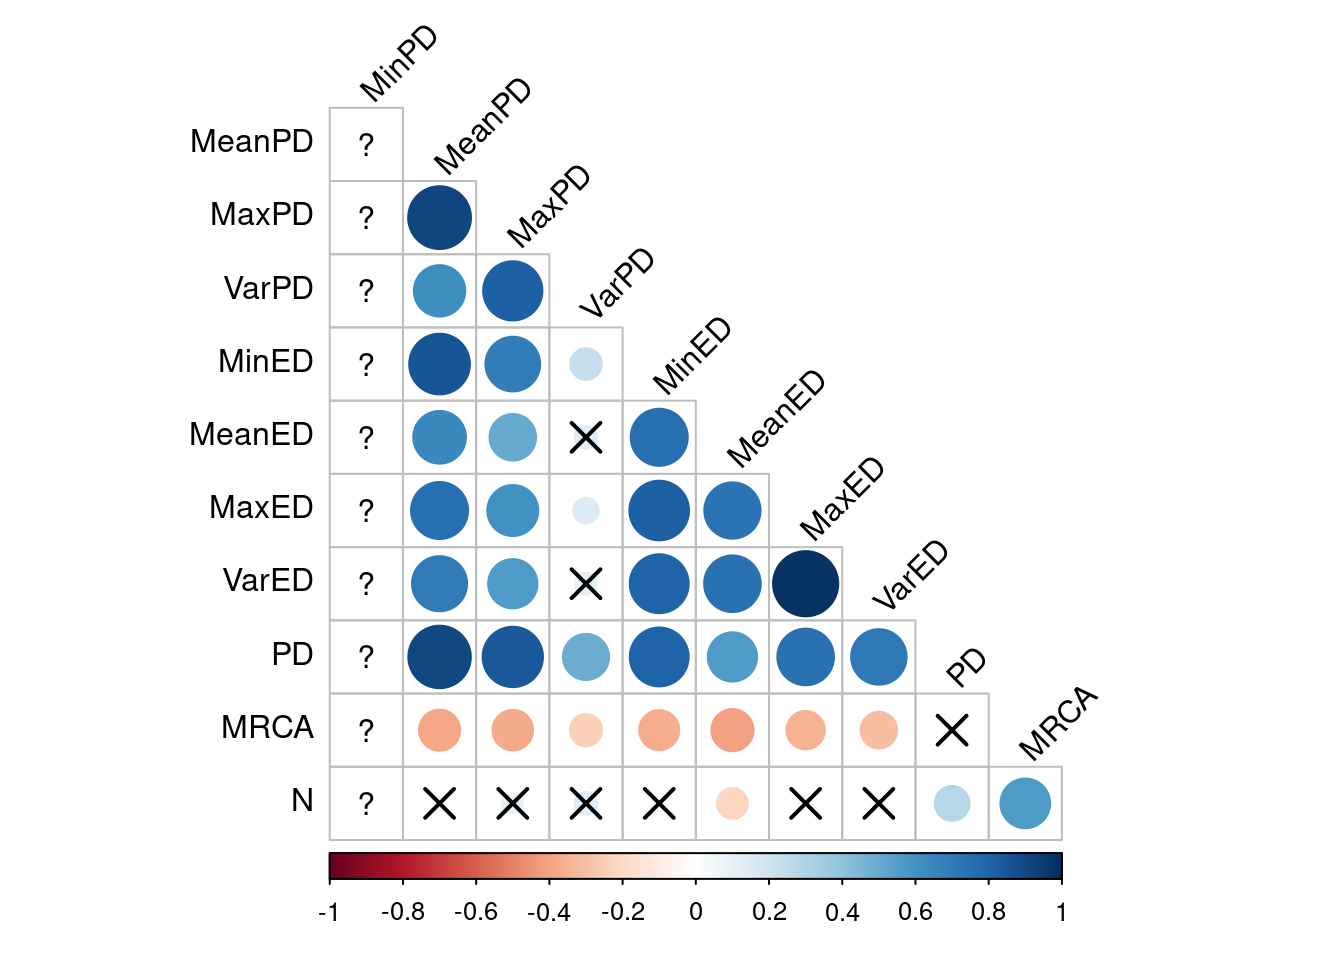
\includegraphics{phylodiversity-in-EC-supplement_files/figure-latex/phylodiversity_correlation_plot-1.pdf}

However, these correlations may well vary by selection scheme, and even over time within a selection scheme. Let's take a look at some scatter plots.

\begin{Shaded}
\begin{Highlighting}[]
\KeywordTok{ggplot}\NormalTok{(}
\NormalTok{    data }\OperatorTok\StringTok{ }\KeywordTok{filter}\NormalTok{(gen}\OperatorTok{==}\DecValTok{500000}\NormalTok{),}
    \KeywordTok{aes}\NormalTok{(}
        \DataTypeTok{y=}\NormalTok{mean_phenotype_pairwise_distance,}
        \DataTypeTok{x=}\NormalTok{variance_phenotype_pairwise_distance,}
        \DataTypeTok{color=}\NormalTok{selection_name,}
        \DataTypeTok{fill=}\NormalTok{selection_name}
\NormalTok{    )}
\NormalTok{  ) }\OperatorTok{+}
\StringTok{  }\KeywordTok{geom_point}\NormalTok{() }\OperatorTok{+}
\StringTok{  }\KeywordTok{scale_x_continuous}\NormalTok{(}
        \DataTypeTok{breaks =} \KeywordTok{breaks_extended}\NormalTok{(}\DecValTok{4}\NormalTok{)}
\NormalTok{  ) }\OperatorTok{+}\StringTok{ }
\StringTok{  }\KeywordTok{facet_wrap}\NormalTok{(}
      \OperatorTok{~}\NormalTok{selection_name, }\DataTypeTok{scales=}\StringTok{"free"}
\NormalTok{  ) }\OperatorTok{+}\StringTok{ }
\StringTok{  }\KeywordTok{stat_smooth}\NormalTok{(}
    \DataTypeTok{method=}\StringTok{"lm"}
\NormalTok{  ) }\OperatorTok{+}\StringTok{ }
\StringTok{  }\KeywordTok{stat_cor}\NormalTok{(}
    \DataTypeTok{method=}\StringTok{"spearman"}\NormalTok{, }\DataTypeTok{cor.coef.name =} \StringTok{"rho"}\NormalTok{, }\DataTypeTok{color=}\StringTok{"black"}
\NormalTok{  ) }\OperatorTok{+}
\StringTok{  }\KeywordTok{theme}\NormalTok{(}\DataTypeTok{legend.position =} \StringTok{"none"}\NormalTok{)}
\end{Highlighting}
\end{Shaded}

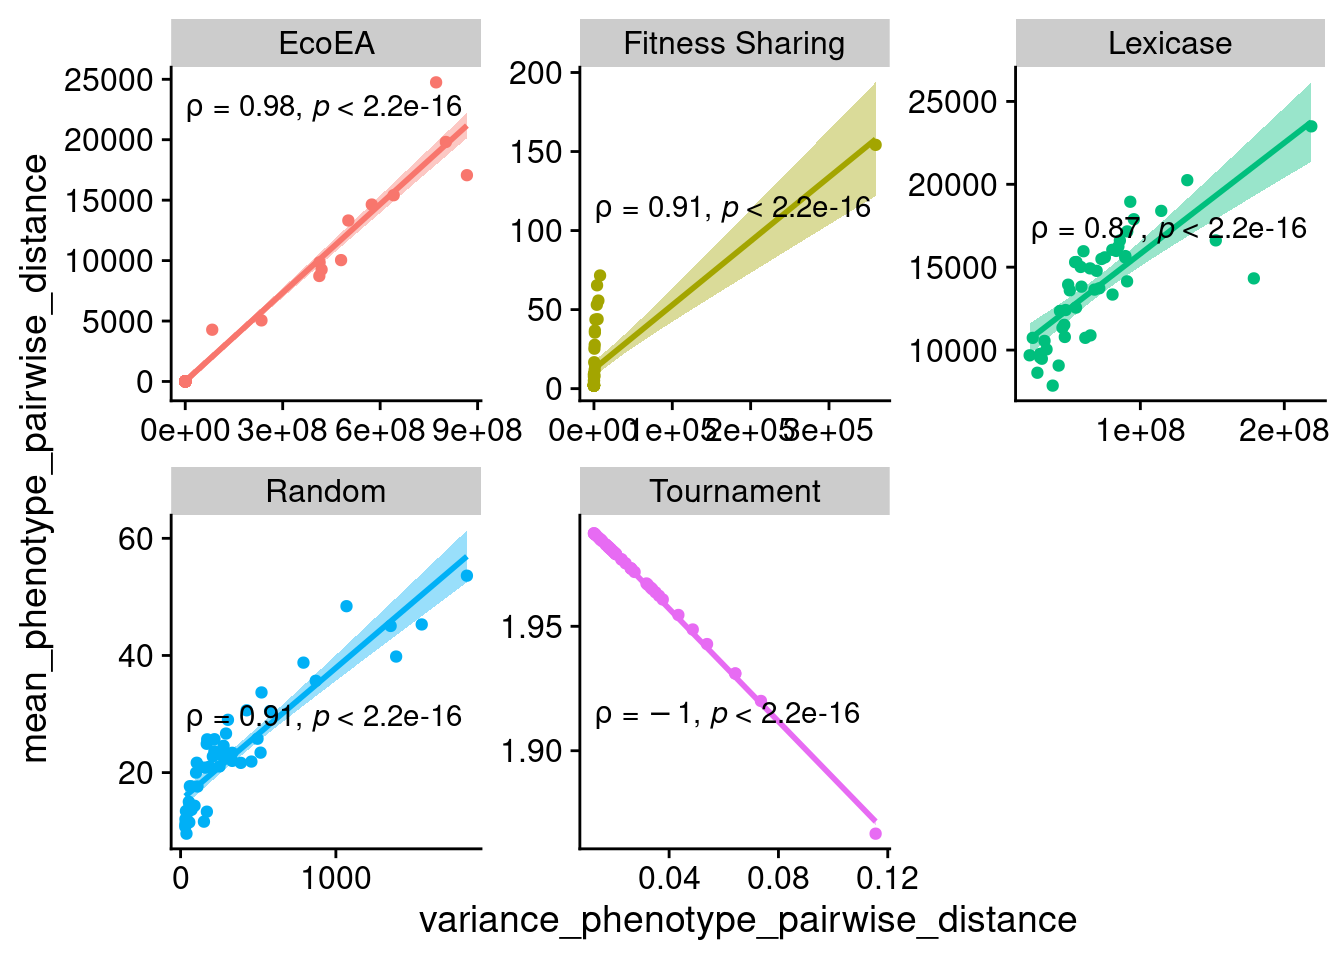
\includegraphics{phylodiversity-in-EC-supplement_files/figure-latex/meanpd_vs_varpd-1.pdf}

Mean and variance of pairwise distances appears to correlate fairly closely with each other across selection schemes. The exception to this is tournament selection, where the range of values for both of these metrics are very small and the correlation is directly inverse. This is likely being driven by there being a small number of taxa that are mostly siblings of each other.

\begin{Shaded}
\begin{Highlighting}[]
\KeywordTok{ggplot}\NormalTok{(}
\NormalTok{    data }\OperatorTok\StringTok{ }\KeywordTok{filter}\NormalTok{(gen}\OperatorTok{==}\DecValTok{500000}\NormalTok{),}
    \KeywordTok{aes}\NormalTok{(}
        \DataTypeTok{y=}\NormalTok{mean_phenotype_pairwise_distance,}
        \DataTypeTok{x=}\NormalTok{max_phenotype_pairwise_distance,}
        \DataTypeTok{color=}\NormalTok{selection_name,}
        \DataTypeTok{fill=}\NormalTok{selection_name}
\NormalTok{    )}
\NormalTok{  ) }\OperatorTok{+}
\StringTok{  }\KeywordTok{geom_point}\NormalTok{() }\OperatorTok{+}
\StringTok{  }\KeywordTok{scale_x_continuous}\NormalTok{(}
        \DataTypeTok{breaks =} \KeywordTok{breaks_extended}\NormalTok{(}\DecValTok{4}\NormalTok{)}
\NormalTok{  ) }\OperatorTok{+}\StringTok{ }
\StringTok{  }\KeywordTok{facet_wrap}\NormalTok{(}
      \OperatorTok{~}\NormalTok{selection_name, }\DataTypeTok{scales=}\StringTok{"free"}
\NormalTok{  ) }\OperatorTok{+}\StringTok{ }
\StringTok{  }\KeywordTok{stat_smooth}\NormalTok{(}
    \DataTypeTok{method=}\StringTok{"lm"}
\NormalTok{  ) }\OperatorTok{+}\StringTok{ }
\StringTok{  }\KeywordTok{stat_cor}\NormalTok{(}
    \DataTypeTok{method=}\StringTok{"spearman"}\NormalTok{, }\DataTypeTok{cor.coef.name =} \StringTok{"rho"}\NormalTok{, }\DataTypeTok{color=}\StringTok{"black"}
\NormalTok{  ) }\OperatorTok{+}
\StringTok{  }\KeywordTok{theme}\NormalTok{(}\DataTypeTok{legend.position =} \StringTok{"none"}\NormalTok{)}
\end{Highlighting}
\end{Shaded}

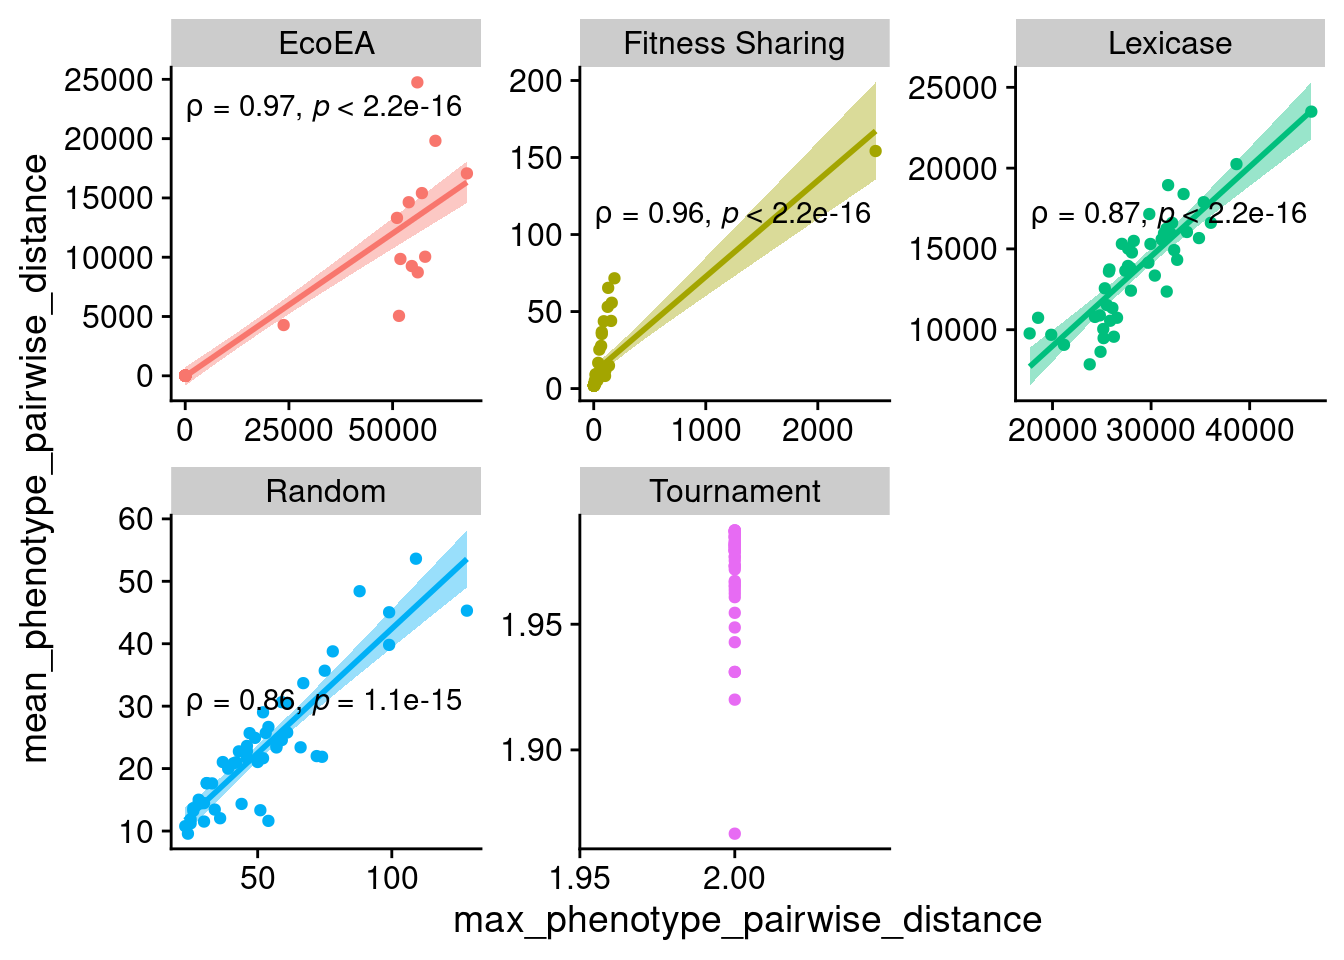
\includegraphics{phylodiversity-in-EC-supplement_files/figure-latex/meanpd_vs_maxpd-1.pdf}

Maximum and mean pairwise distance also correlate pretty closely, with the exception again being tournament. These data shed further light on the previous graph as well - the maximum pariwise distance for tournament selection is always 2.

\begin{Shaded}
\begin{Highlighting}[]
\KeywordTok{ggplot}\NormalTok{(}
\NormalTok{    data }\OperatorTok\StringTok{ }\KeywordTok{filter}\NormalTok{(gen}\OperatorTok{==}\DecValTok{500000}\NormalTok{),}
    \KeywordTok{aes}\NormalTok{(}
        \DataTypeTok{y=}\NormalTok{variance_phenotype_pairwise_distance,}
        \DataTypeTok{x=}\NormalTok{max_phenotype_pairwise_distance,}
        \DataTypeTok{color=}\NormalTok{selection_name,}
        \DataTypeTok{fill=}\NormalTok{selection_name}
\NormalTok{    )}
\NormalTok{  ) }\OperatorTok{+}
\StringTok{  }\KeywordTok{geom_point}\NormalTok{() }\OperatorTok{+}
\StringTok{  }\KeywordTok{scale_x_continuous}\NormalTok{(}
        \DataTypeTok{breaks =} \KeywordTok{breaks_extended}\NormalTok{(}\DecValTok{4}\NormalTok{)}
\NormalTok{  ) }\OperatorTok{+}\StringTok{ }
\StringTok{  }\KeywordTok{facet_wrap}\NormalTok{(}
      \OperatorTok{~}\NormalTok{selection_name, }\DataTypeTok{scales=}\StringTok{"free"}
\NormalTok{  ) }\OperatorTok{+}\StringTok{ }
\StringTok{  }\KeywordTok{stat_smooth}\NormalTok{(}
    \DataTypeTok{method=}\StringTok{"lm"}
\NormalTok{  ) }\OperatorTok{+}\StringTok{ }
\StringTok{  }\KeywordTok{stat_cor}\NormalTok{(}
    \DataTypeTok{method=}\StringTok{"spearman"}\NormalTok{, }\DataTypeTok{cor.coef.name =} \StringTok{"rho"}\NormalTok{, }\DataTypeTok{color=}\StringTok{"black"}
\NormalTok{  ) }\OperatorTok{+}
\StringTok{  }\KeywordTok{theme}\NormalTok{(}\DataTypeTok{legend.position =} \StringTok{"none"}\NormalTok{)}
\end{Highlighting}
\end{Shaded}

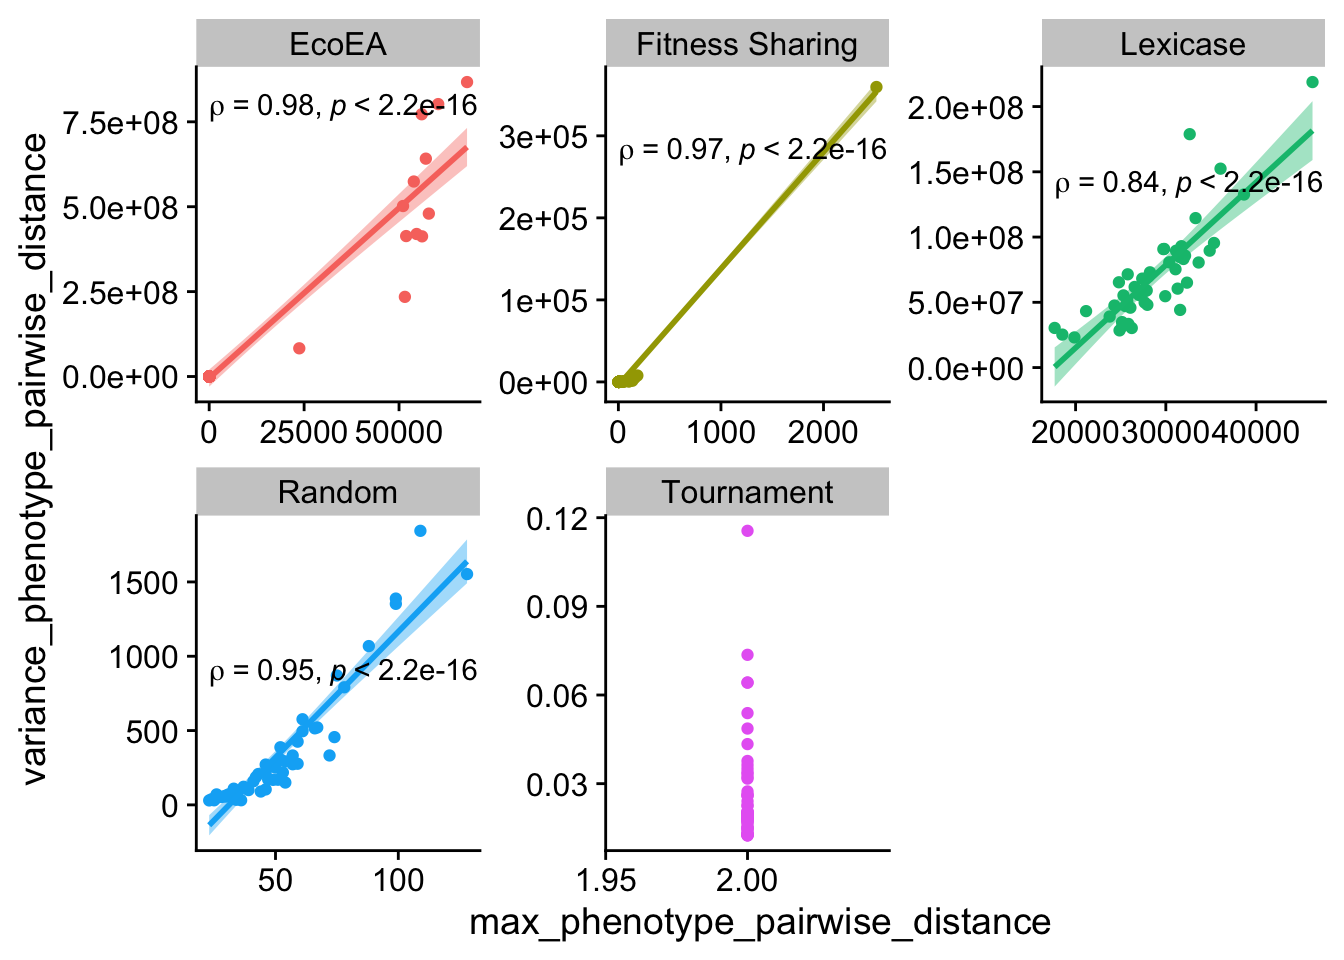
\includegraphics{phylodiversity-in-EC-supplement_files/figure-latex/varpd_vs_maxpd-1.pdf}

Max and variance of pairwise distances behave similarly.

And let's check that it doesn't look radically different early on in the run:

\begin{Shaded}
\begin{Highlighting}[]
\KeywordTok{ggplot}\NormalTok{(}
\NormalTok{    data }\OperatorTok\StringTok{ }\KeywordTok{filter}\NormalTok{(gen}\OperatorTok{==}\DecValTok{5000}\NormalTok{),}
    \KeywordTok{aes}\NormalTok{(}
        \DataTypeTok{y=}\NormalTok{mean_phenotype_pairwise_distance,}
        \DataTypeTok{x=}\NormalTok{variance_phenotype_pairwise_distance,}
        \DataTypeTok{color=}\NormalTok{selection_name,}
        \DataTypeTok{fill=}\NormalTok{selection_name}
\NormalTok{    )}
\NormalTok{  ) }\OperatorTok{+}
\StringTok{  }\KeywordTok{geom_point}\NormalTok{() }\OperatorTok{+}
\StringTok{  }\KeywordTok{scale_x_continuous}\NormalTok{(}
        \DataTypeTok{breaks =} \KeywordTok{breaks_extended}\NormalTok{(}\DecValTok{4}\NormalTok{)}
\NormalTok{  ) }\OperatorTok{+}\StringTok{ }
\StringTok{  }\KeywordTok{facet_wrap}\NormalTok{(}
      \OperatorTok{~}\NormalTok{selection_name, }\DataTypeTok{scales=}\StringTok{"free"}
\NormalTok{  ) }\OperatorTok{+}\StringTok{ }
\StringTok{  }\KeywordTok{stat_smooth}\NormalTok{(}
    \DataTypeTok{method=}\StringTok{"lm"}
\NormalTok{  ) }\OperatorTok{+}\StringTok{ }
\StringTok{  }\KeywordTok{stat_cor}\NormalTok{(}
    \DataTypeTok{method=}\StringTok{"spearman"}\NormalTok{, }\DataTypeTok{cor.coef.name =} \StringTok{"rho"}\NormalTok{, }\DataTypeTok{color=}\StringTok{"black"}
\NormalTok{  ) }\OperatorTok{+}
\StringTok{  }\KeywordTok{theme}\NormalTok{(}\DataTypeTok{legend.position =} \StringTok{"none"}\NormalTok{)}
\end{Highlighting}
\end{Shaded}

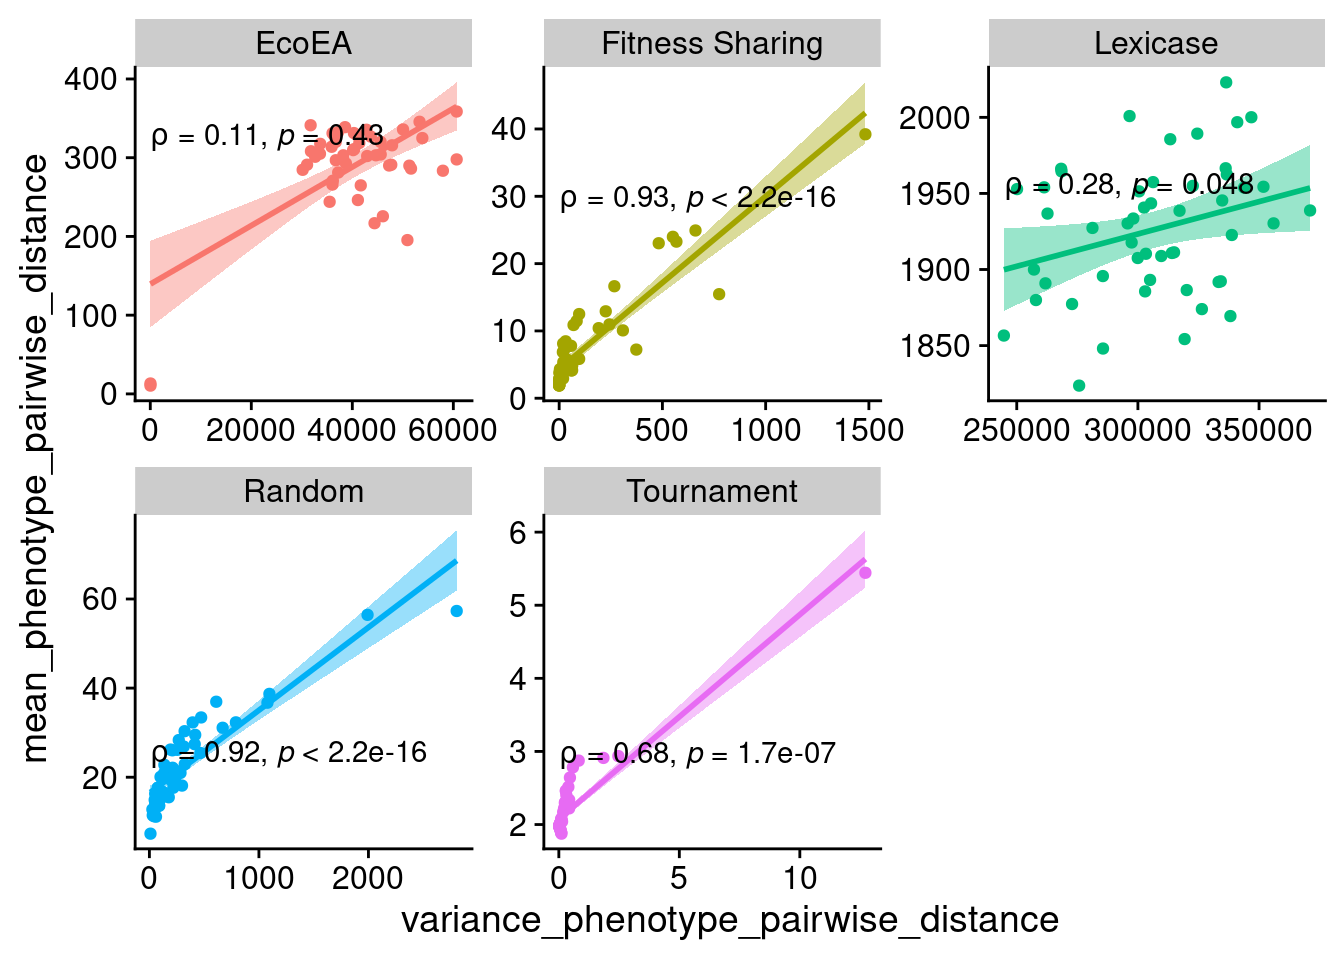
\includegraphics{phylodiversity-in-EC-supplement_files/figure-latex/meanpd_vs_varpd_early-1.pdf}

The correlation between these two metrics is substantially weaker for Eco-Ea and lexicase selection at the early time point.

\begin{Shaded}
\begin{Highlighting}[]
\KeywordTok{ggplot}\NormalTok{(}
\NormalTok{    data }\OperatorTok\StringTok{ }\KeywordTok{filter}\NormalTok{(gen}\OperatorTok{==}\DecValTok{5000}\NormalTok{),}
    \KeywordTok{aes}\NormalTok{(}
        \DataTypeTok{y=}\NormalTok{mean_phenotype_pairwise_distance,}
        \DataTypeTok{x=}\NormalTok{max_phenotype_pairwise_distance,}
        \DataTypeTok{color=}\NormalTok{selection_name,}
        \DataTypeTok{fill=}\NormalTok{selection_name}
\NormalTok{    )}
\NormalTok{  ) }\OperatorTok{+}
\StringTok{  }\KeywordTok{geom_point}\NormalTok{() }\OperatorTok{+}
\StringTok{  }\KeywordTok{scale_x_continuous}\NormalTok{(}
        \DataTypeTok{breaks =} \KeywordTok{breaks_extended}\NormalTok{(}\DecValTok{4}\NormalTok{)}
\NormalTok{  ) }\OperatorTok{+}\StringTok{ }
\StringTok{  }\KeywordTok{facet_wrap}\NormalTok{(}
      \OperatorTok{~}\NormalTok{selection_name, }\DataTypeTok{scales=}\StringTok{"free"}
\NormalTok{  ) }\OperatorTok{+}\StringTok{ }
\StringTok{  }\KeywordTok{stat_smooth}\NormalTok{(}
    \DataTypeTok{method=}\StringTok{"lm"}
\NormalTok{  ) }\OperatorTok{+}\StringTok{ }
\StringTok{  }\KeywordTok{stat_cor}\NormalTok{(}
    \DataTypeTok{method=}\StringTok{"spearman"}\NormalTok{, }\DataTypeTok{cor.coef.name =} \StringTok{"rho"}\NormalTok{, }\DataTypeTok{color=}\StringTok{"black"}
\NormalTok{  ) }\OperatorTok{+}
\StringTok{  }\KeywordTok{theme}\NormalTok{(}\DataTypeTok{legend.position =} \StringTok{"none"}\NormalTok{)}
\end{Highlighting}
\end{Shaded}

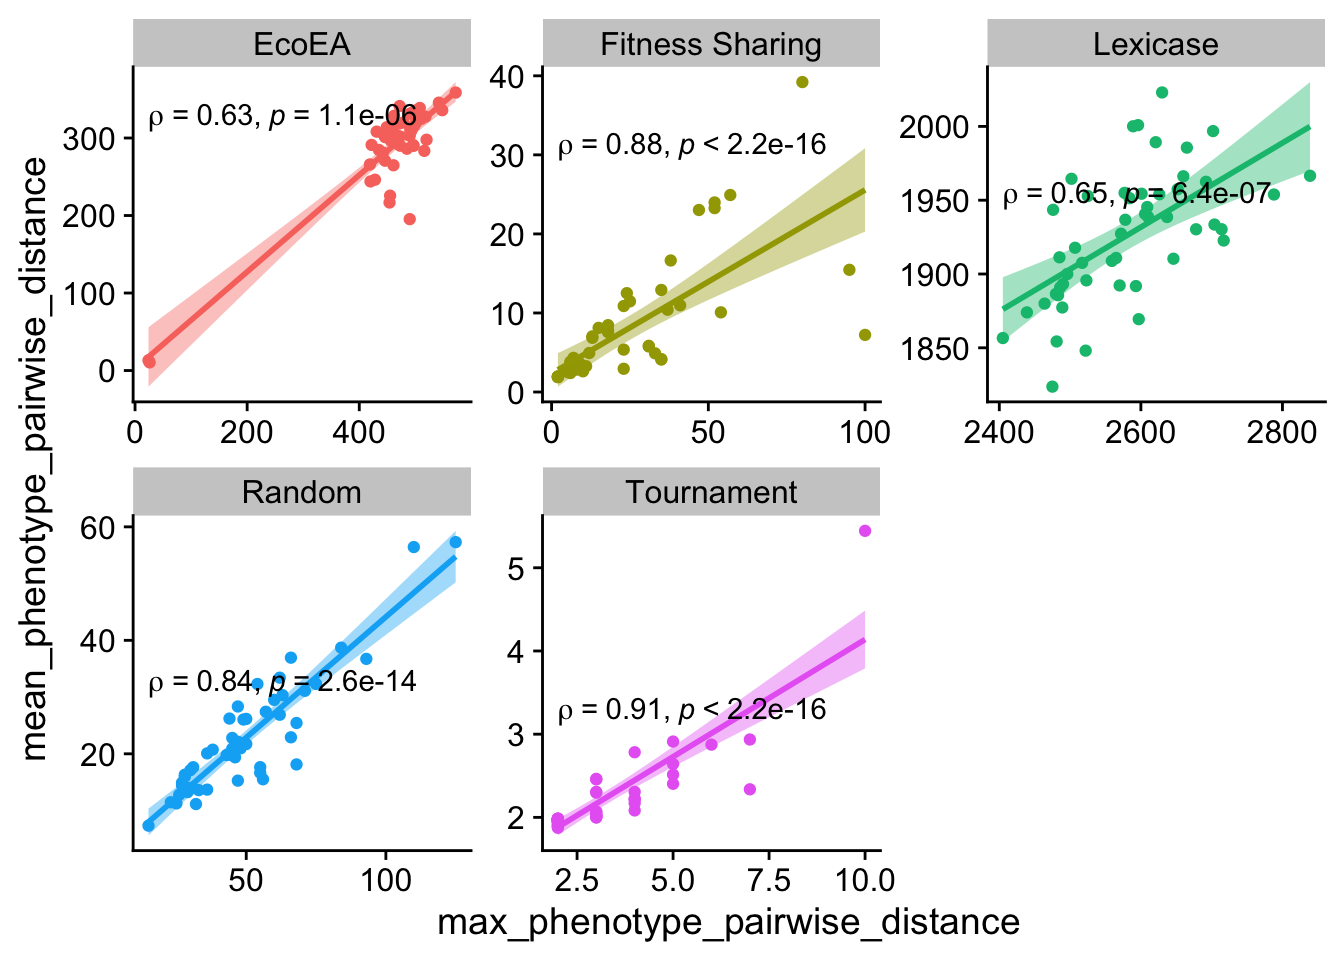
\includegraphics{phylodiversity-in-EC-supplement_files/figure-latex/meanpd_vs_maxpd_early-1.pdf}

This relationship is also weaker, although not as much weaker.

\begin{Shaded}
\begin{Highlighting}[]
\KeywordTok{ggplot}\NormalTok{(}
\NormalTok{    data }\OperatorTok\StringTok{ }\KeywordTok{filter}\NormalTok{(gen}\OperatorTok{==}\DecValTok{5000}\NormalTok{),}
    \KeywordTok{aes}\NormalTok{(}
        \DataTypeTok{y=}\NormalTok{variance_phenotype_pairwise_distance,}
        \DataTypeTok{x=}\NormalTok{max_phenotype_pairwise_distance,}
        \DataTypeTok{color=}\NormalTok{selection_name,}
        \DataTypeTok{fill=}\NormalTok{selection_name}
\NormalTok{    )}
\NormalTok{  ) }\OperatorTok{+}
\StringTok{  }\KeywordTok{geom_point}\NormalTok{() }\OperatorTok{+}
\StringTok{  }\KeywordTok{scale_x_continuous}\NormalTok{(}
        \DataTypeTok{breaks =} \KeywordTok{breaks_extended}\NormalTok{(}\DecValTok{4}\NormalTok{)}
\NormalTok{  ) }\OperatorTok{+}\StringTok{ }
\StringTok{  }\KeywordTok{facet_wrap}\NormalTok{(}
      \OperatorTok{~}\NormalTok{selection_name, }\DataTypeTok{scales=}\StringTok{"free"}
\NormalTok{  ) }\OperatorTok{+}\StringTok{ }
\StringTok{  }\KeywordTok{stat_smooth}\NormalTok{(}
    \DataTypeTok{method=}\StringTok{"lm"}
\NormalTok{  ) }\OperatorTok{+}\StringTok{ }
\StringTok{  }\KeywordTok{stat_cor}\NormalTok{(}
    \DataTypeTok{method=}\StringTok{"spearman"}\NormalTok{, }\DataTypeTok{cor.coef.name =} \StringTok{"rho"}\NormalTok{, }\DataTypeTok{color=}\StringTok{"black"}
\NormalTok{  ) }\OperatorTok{+}
\StringTok{  }\KeywordTok{theme}\NormalTok{(}\DataTypeTok{legend.position =} \StringTok{"none"}\NormalTok{)}
\end{Highlighting}
\end{Shaded}

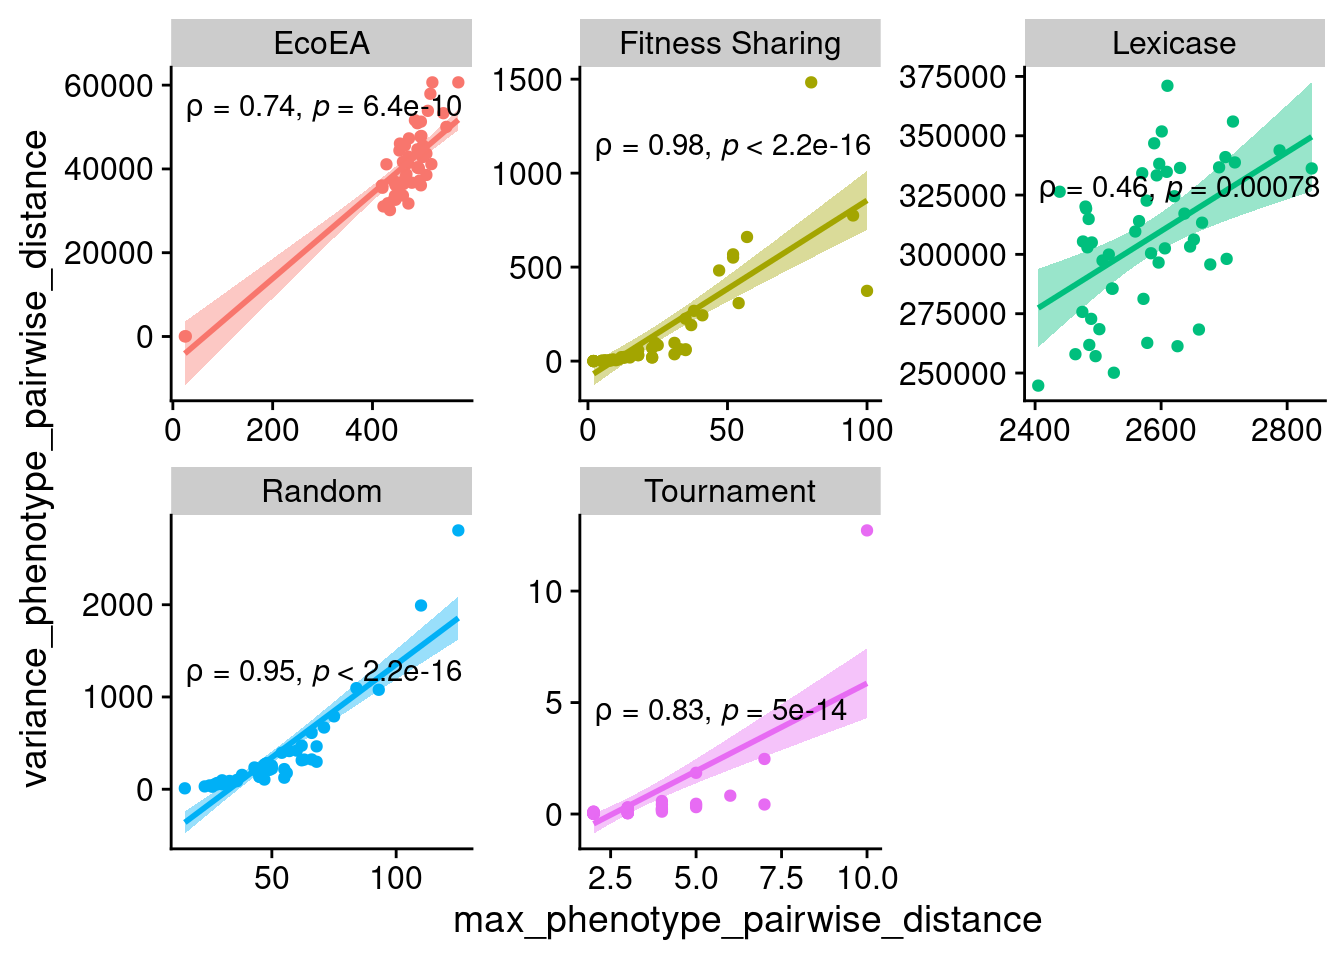
\includegraphics{phylodiversity-in-EC-supplement_files/figure-latex/varpd_vs_maxpd_early-1.pdf}

Similarly, the correlation between max and variance of pariwise distances is weakend, but still robust. So the relationship between mean and variance of pairwise distances is the only one that is really weaker at the earlier time points. Understanding exactly what drives these discrepancies is a promising angle for future work, as it may shed further light on the dynamics occurring in the run. It is particularly interesting that EcoEA and Lexicase selection are the scenarios where they diverge.

Similarly, the evolutionary distinctiveness metrics look largely similar to each other, but let's spot check that too.

\begin{Shaded}
\begin{Highlighting}[]
\KeywordTok{ggplot}\NormalTok{(}
\NormalTok{    data }\OperatorTok\StringTok{ }\KeywordTok{filter}\NormalTok{(gen}\OperatorTok{==}\DecValTok{500000}\NormalTok{),}
    \KeywordTok{aes}\NormalTok{(}
        \DataTypeTok{y=}\NormalTok{mean_phenotype_evolutionary_distinctiveness,}
        \DataTypeTok{x=}\NormalTok{variance_phenotype_evolutionary_distinctiveness,}
        \DataTypeTok{color=}\NormalTok{selection_name,}
        \DataTypeTok{fill=}\NormalTok{selection_name}
\NormalTok{    )}
\NormalTok{  ) }\OperatorTok{+}
\StringTok{  }\KeywordTok{geom_point}\NormalTok{() }\OperatorTok{+}
\StringTok{  }\KeywordTok{scale_x_continuous}\NormalTok{(}
        \DataTypeTok{breaks =} \KeywordTok{breaks_extended}\NormalTok{(}\DecValTok{4}\NormalTok{)}
\NormalTok{  ) }\OperatorTok{+}\StringTok{ }
\StringTok{  }\KeywordTok{facet_wrap}\NormalTok{(}
      \OperatorTok{~}\NormalTok{selection_name, }\DataTypeTok{scales=}\StringTok{"free"}
\NormalTok{  ) }\OperatorTok{+}\StringTok{ }
\StringTok{  }\KeywordTok{stat_smooth}\NormalTok{(}
    \DataTypeTok{method=}\StringTok{"lm"}
\NormalTok{  ) }\OperatorTok{+}\StringTok{ }
\StringTok{  }\KeywordTok{stat_cor}\NormalTok{(}
    \DataTypeTok{method=}\StringTok{"spearman"}\NormalTok{, }\DataTypeTok{cor.coef.name =} \StringTok{"rho"}\NormalTok{, }\DataTypeTok{color=}\StringTok{"black"}
\NormalTok{  ) }\OperatorTok{+}
\StringTok{  }\KeywordTok{theme}\NormalTok{(}\DataTypeTok{legend.position =} \StringTok{"none"}\NormalTok{)}
\end{Highlighting}
\end{Shaded}

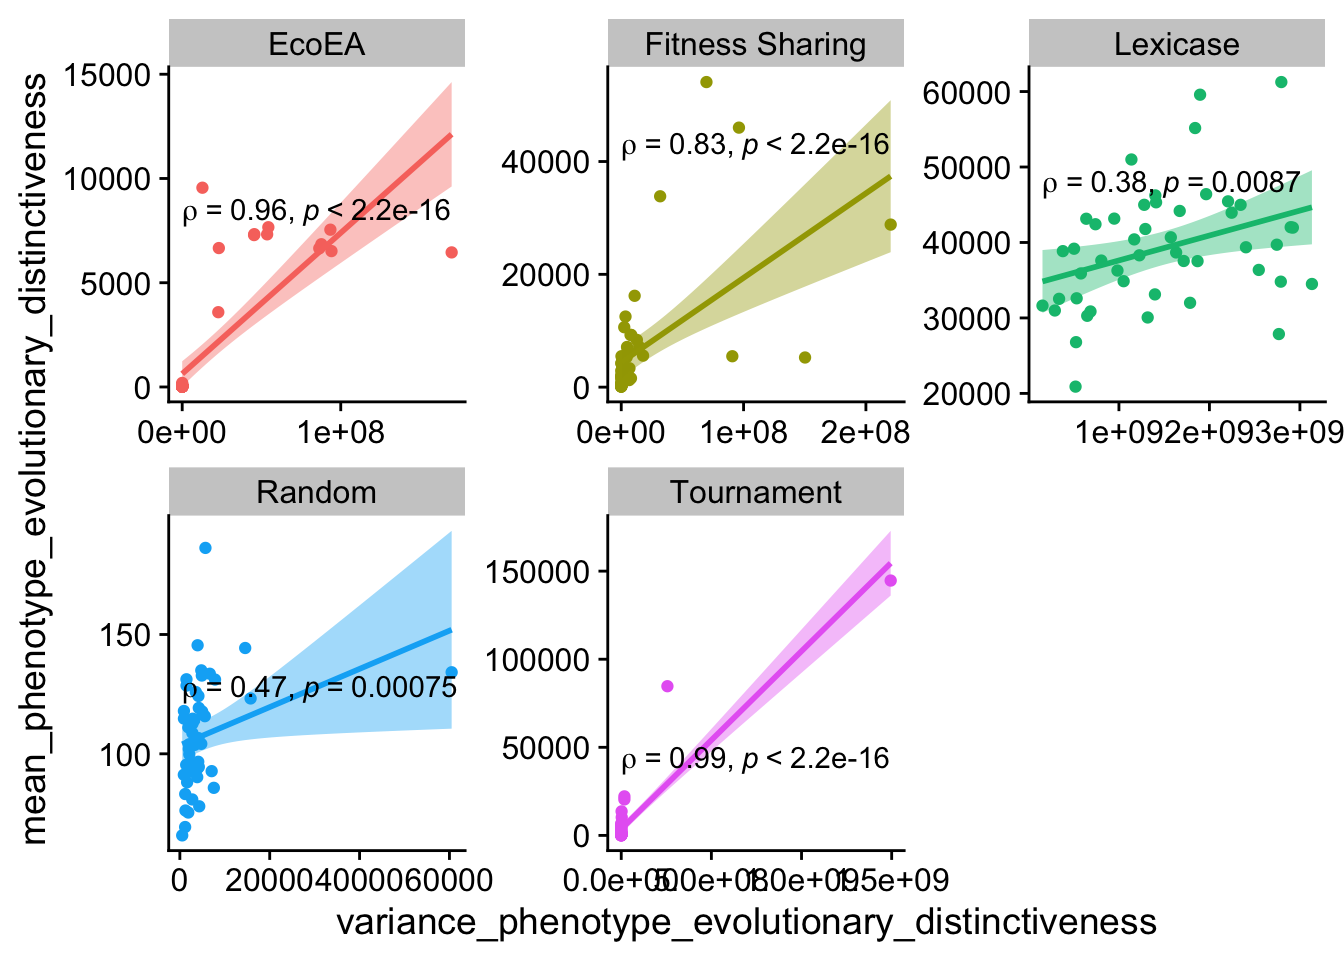
\includegraphics{phylodiversity-in-EC-supplement_files/figure-latex/med_vs_ved-1.pdf}

These aren't the strongest correlations; different information is definitely being captured by each metric. However, they still correlate to a fair extent.

\begin{Shaded}
\begin{Highlighting}[]
\KeywordTok{ggplot}\NormalTok{(}
\NormalTok{    data }\OperatorTok\StringTok{ }\KeywordTok{filter}\NormalTok{(gen}\OperatorTok{==}\DecValTok{500000}\NormalTok{),}
    \KeywordTok{aes}\NormalTok{(}
        \DataTypeTok{y=}\NormalTok{mean_phenotype_evolutionary_distinctiveness,}
        \DataTypeTok{x=}\NormalTok{max_phenotype_evolutionary_distinctiveness,}
        \DataTypeTok{color=}\NormalTok{selection_name,}
        \DataTypeTok{fill=}\NormalTok{selection_name}
\NormalTok{    )}
\NormalTok{  ) }\OperatorTok{+}
\StringTok{  }\KeywordTok{geom_point}\NormalTok{() }\OperatorTok{+}
\StringTok{  }\KeywordTok{scale_x_continuous}\NormalTok{(}
        \DataTypeTok{breaks =} \KeywordTok{breaks_extended}\NormalTok{(}\DecValTok{4}\NormalTok{)}
\NormalTok{  ) }\OperatorTok{+}\StringTok{ }
\StringTok{  }\KeywordTok{facet_wrap}\NormalTok{(}
      \OperatorTok{~}\NormalTok{selection_name, }\DataTypeTok{scales=}\StringTok{"free"}
\NormalTok{  ) }\OperatorTok{+}\StringTok{ }
\StringTok{  }\KeywordTok{stat_smooth}\NormalTok{(}
    \DataTypeTok{method=}\StringTok{"lm"}
\NormalTok{  ) }\OperatorTok{+}\StringTok{ }
\StringTok{  }\KeywordTok{stat_cor}\NormalTok{(}
    \DataTypeTok{method=}\StringTok{"spearman"}\NormalTok{, }\DataTypeTok{cor.coef.name =} \StringTok{"rho"}\NormalTok{, }\DataTypeTok{color=}\StringTok{"black"}
\NormalTok{  ) }\OperatorTok{+}
\StringTok{  }\KeywordTok{theme}\NormalTok{(}\DataTypeTok{legend.position =} \StringTok{"none"}\NormalTok{)}
\end{Highlighting}
\end{Shaded}

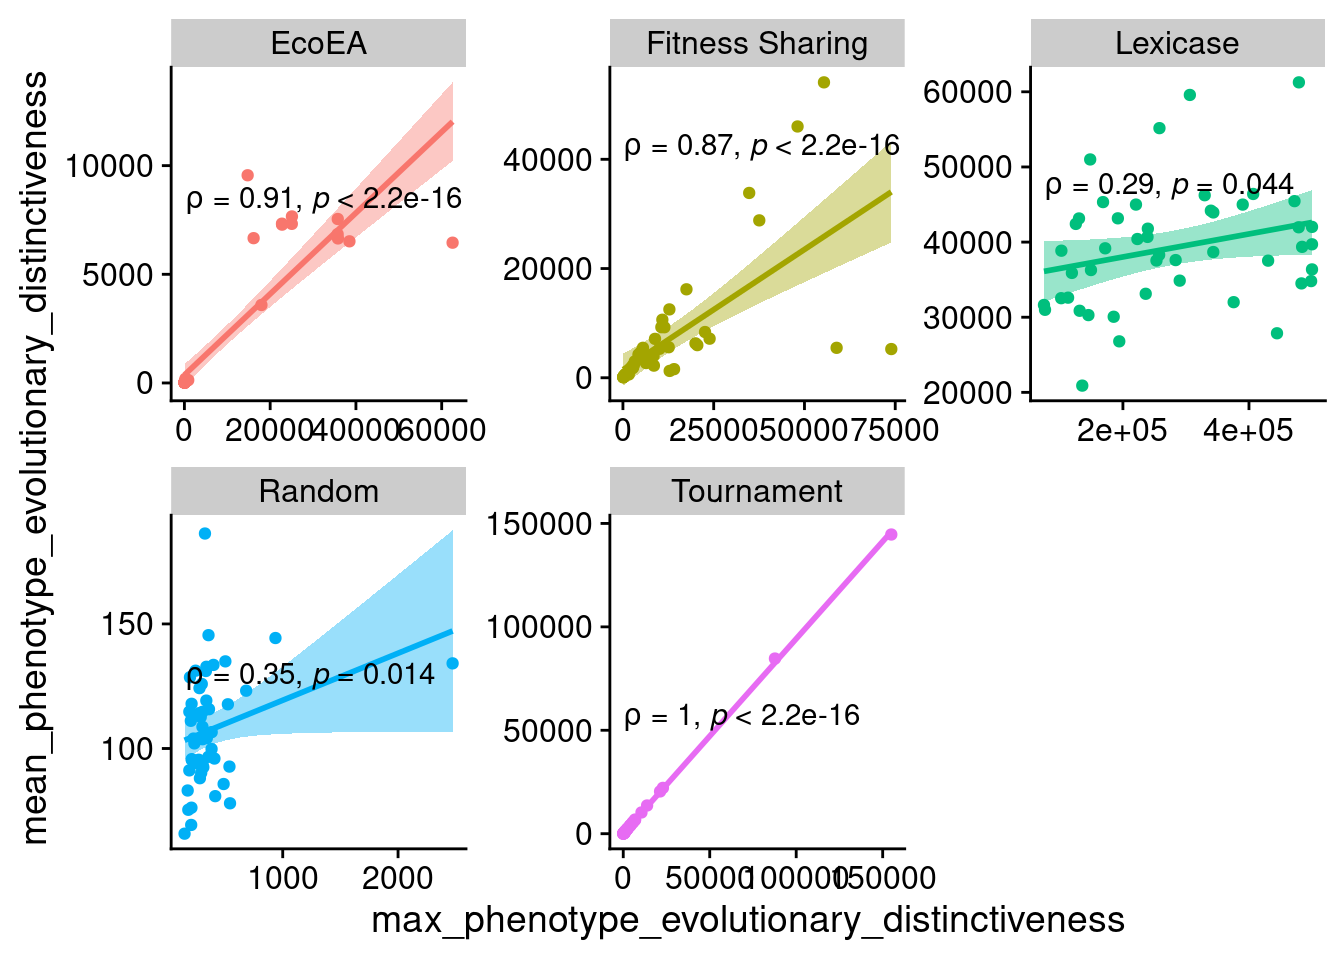
\includegraphics{phylodiversity-in-EC-supplement_files/figure-latex/med_vs_max_ed-1.pdf}

Again, for the most part there is a fairly high degree of correlation here.

\begin{Shaded}
\begin{Highlighting}[]
\KeywordTok{ggplot}\NormalTok{(}
\NormalTok{    data }\OperatorTok\StringTok{ }\KeywordTok{filter}\NormalTok{(gen}\OperatorTok{==}\DecValTok{500000}\NormalTok{),}
    \KeywordTok{aes}\NormalTok{(}
        \DataTypeTok{y=}\NormalTok{mean_phenotype_evolutionary_distinctiveness,}
        \DataTypeTok{x=}\NormalTok{min_phenotype_evolutionary_distinctiveness,}
        \DataTypeTok{color=}\NormalTok{selection_name,}
        \DataTypeTok{fill=}\NormalTok{selection_name}
\NormalTok{    )}
\NormalTok{  ) }\OperatorTok{+}
\StringTok{  }\KeywordTok{geom_point}\NormalTok{() }\OperatorTok{+}
\StringTok{  }\KeywordTok{scale_x_continuous}\NormalTok{(}
        \DataTypeTok{breaks =} \KeywordTok{breaks_extended}\NormalTok{(}\DecValTok{4}\NormalTok{)}
\NormalTok{  ) }\OperatorTok{+}\StringTok{ }
\StringTok{  }\KeywordTok{facet_wrap}\NormalTok{(}
      \OperatorTok{~}\NormalTok{selection_name, }\DataTypeTok{scales=}\StringTok{"free"}
\NormalTok{  ) }\OperatorTok{+}\StringTok{ }
\StringTok{  }\KeywordTok{stat_smooth}\NormalTok{(}
    \DataTypeTok{method=}\StringTok{"lm"}
\NormalTok{  ) }\OperatorTok{+}\StringTok{ }
\StringTok{  }\KeywordTok{stat_cor}\NormalTok{(}
    \DataTypeTok{method=}\StringTok{"spearman"}\NormalTok{, }\DataTypeTok{cor.coef.name =} \StringTok{"rho"}\NormalTok{, }\DataTypeTok{color=}\StringTok{"black"}
\NormalTok{  ) }\OperatorTok{+}
\StringTok{  }\KeywordTok{theme}\NormalTok{(}\DataTypeTok{legend.position =} \StringTok{"none"}\NormalTok{)}
\end{Highlighting}
\end{Shaded}

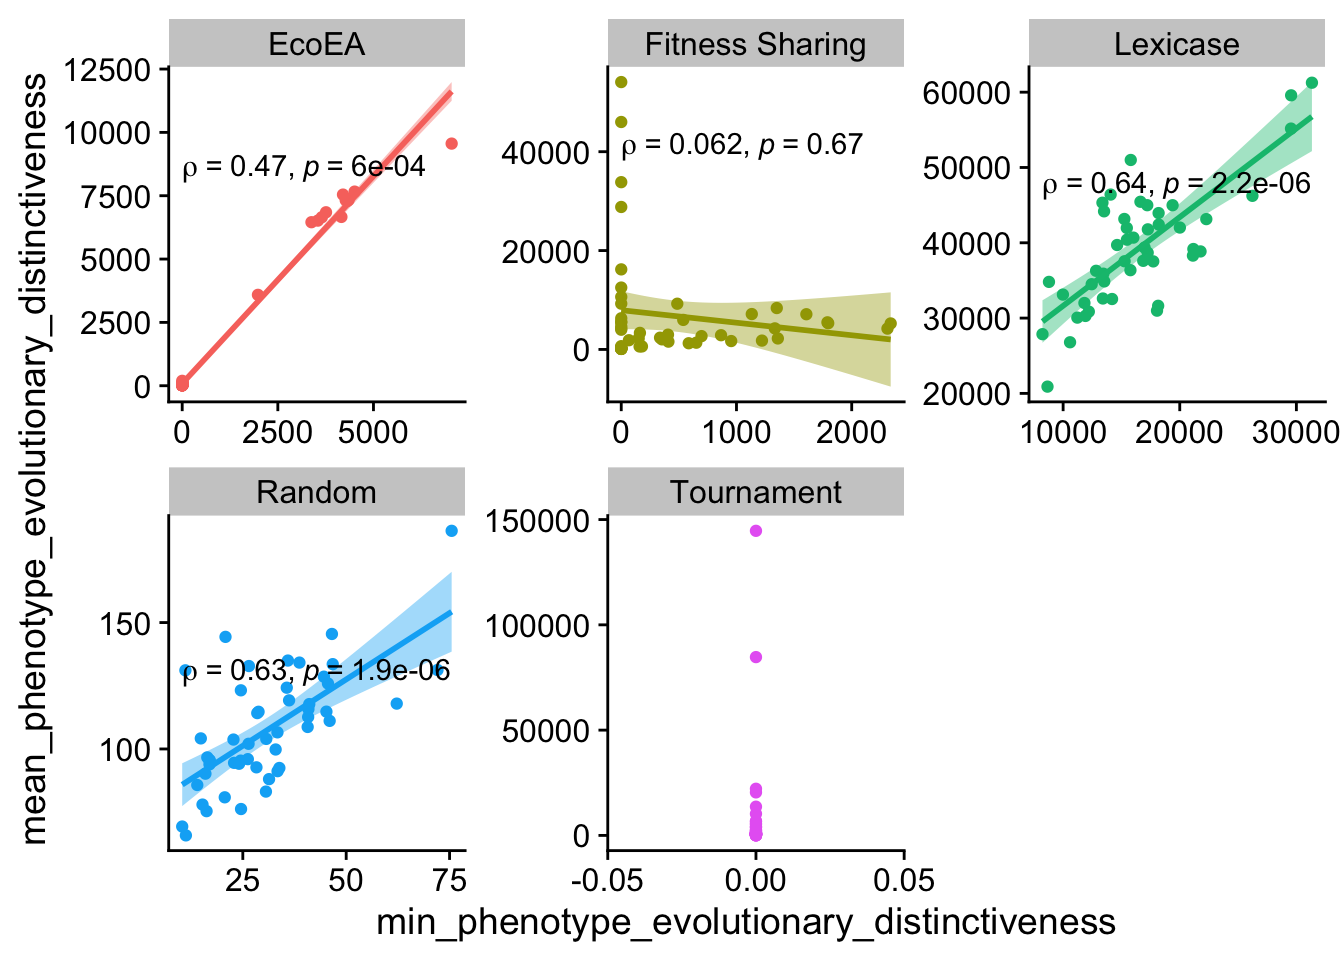
\includegraphics{phylodiversity-in-EC-supplement_files/figure-latex/med_vs_min_ed-1.pdf}

And here too, although it's getting kind of weak for lexicase.

And let's check out an earlier time point

\begin{Shaded}
\begin{Highlighting}[]
\KeywordTok{ggplot}\NormalTok{(}
\NormalTok{    data }\OperatorTok\StringTok{ }\KeywordTok{filter}\NormalTok{(gen}\OperatorTok{==}\DecValTok{5000}\NormalTok{),}
    \KeywordTok{aes}\NormalTok{(}
        \DataTypeTok{y=}\NormalTok{mean_phenotype_evolutionary_distinctiveness,}
        \DataTypeTok{x=}\NormalTok{variance_phenotype_evolutionary_distinctiveness,}
        \DataTypeTok{color=}\NormalTok{selection_name,}
        \DataTypeTok{fill=}\NormalTok{selection_name}
\NormalTok{    )}
\NormalTok{  ) }\OperatorTok{+}
\StringTok{  }\KeywordTok{geom_point}\NormalTok{() }\OperatorTok{+}
\StringTok{  }\KeywordTok{scale_x_continuous}\NormalTok{(}
        \DataTypeTok{breaks =} \KeywordTok{breaks_extended}\NormalTok{(}\DecValTok{4}\NormalTok{)}
\NormalTok{  ) }\OperatorTok{+}\StringTok{ }
\StringTok{  }\KeywordTok{facet_wrap}\NormalTok{(}
      \OperatorTok{~}\NormalTok{selection_name, }\DataTypeTok{scales=}\StringTok{"free"}
\NormalTok{  ) }\OperatorTok{+}\StringTok{ }
\StringTok{  }\KeywordTok{stat_smooth}\NormalTok{(}
    \DataTypeTok{method=}\StringTok{"lm"}
\NormalTok{  ) }\OperatorTok{+}\StringTok{ }
\StringTok{  }\KeywordTok{stat_cor}\NormalTok{(}
    \DataTypeTok{method=}\StringTok{"spearman"}\NormalTok{, }\DataTypeTok{cor.coef.name =} \StringTok{"rho"}\NormalTok{, }\DataTypeTok{color=}\StringTok{"black"}
\NormalTok{  ) }\OperatorTok{+}
\StringTok{  }\KeywordTok{theme}\NormalTok{(}\DataTypeTok{legend.position =} \StringTok{"none"}\NormalTok{)}
\end{Highlighting}
\end{Shaded}

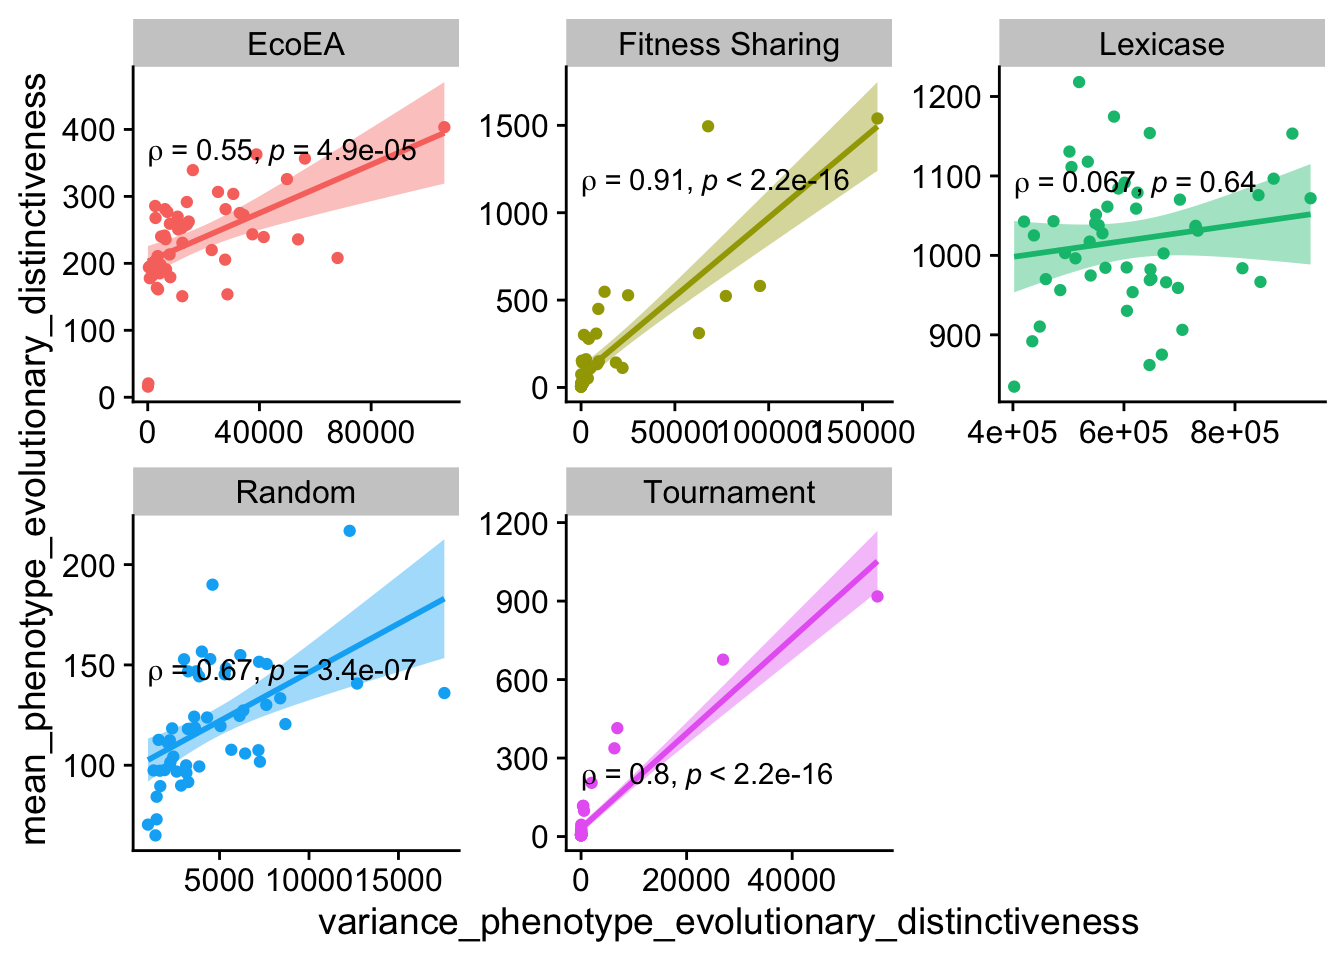
\includegraphics{phylodiversity-in-EC-supplement_files/figure-latex/med_vs_ved_early-1.pdf}

The relationship between min and mean evolutionary distinctiveness holds up at the earlier time point for everything except fitness sharing.

\begin{Shaded}
\begin{Highlighting}[]
\KeywordTok{ggplot}\NormalTok{(}
\NormalTok{    data }\OperatorTok\StringTok{ }\KeywordTok{filter}\NormalTok{(gen}\OperatorTok{==}\DecValTok{5000}\NormalTok{),}
    \KeywordTok{aes}\NormalTok{(}
        \DataTypeTok{y=}\NormalTok{mean_phenotype_evolutionary_distinctiveness,}
        \DataTypeTok{x=}\NormalTok{max_phenotype_evolutionary_distinctiveness,}
        \DataTypeTok{color=}\NormalTok{selection_name,}
        \DataTypeTok{fill=}\NormalTok{selection_name}
\NormalTok{    )}
\NormalTok{  ) }\OperatorTok{+}
\StringTok{  }\KeywordTok{geom_point}\NormalTok{() }\OperatorTok{+}
\StringTok{  }\KeywordTok{scale_x_continuous}\NormalTok{(}
        \DataTypeTok{breaks =} \KeywordTok{breaks_extended}\NormalTok{(}\DecValTok{4}\NormalTok{)}
\NormalTok{  ) }\OperatorTok{+}\StringTok{ }
\StringTok{  }\KeywordTok{facet_wrap}\NormalTok{(}
      \OperatorTok{~}\NormalTok{selection_name, }\DataTypeTok{scales=}\StringTok{"free"}
\NormalTok{  ) }\OperatorTok{+}\StringTok{ }
\StringTok{  }\KeywordTok{stat_smooth}\NormalTok{(}
    \DataTypeTok{method=}\StringTok{"lm"}
\NormalTok{  ) }\OperatorTok{+}\StringTok{ }
\StringTok{  }\KeywordTok{stat_cor}\NormalTok{(}
    \DataTypeTok{method=}\StringTok{"spearman"}\NormalTok{, }\DataTypeTok{cor.coef.name =} \StringTok{"rho"}\NormalTok{, }\DataTypeTok{color=}\StringTok{"black"}
\NormalTok{  ) }\OperatorTok{+}
\StringTok{  }\KeywordTok{theme}\NormalTok{(}\DataTypeTok{legend.position =} \StringTok{"none"}\NormalTok{)}
\end{Highlighting}
\end{Shaded}

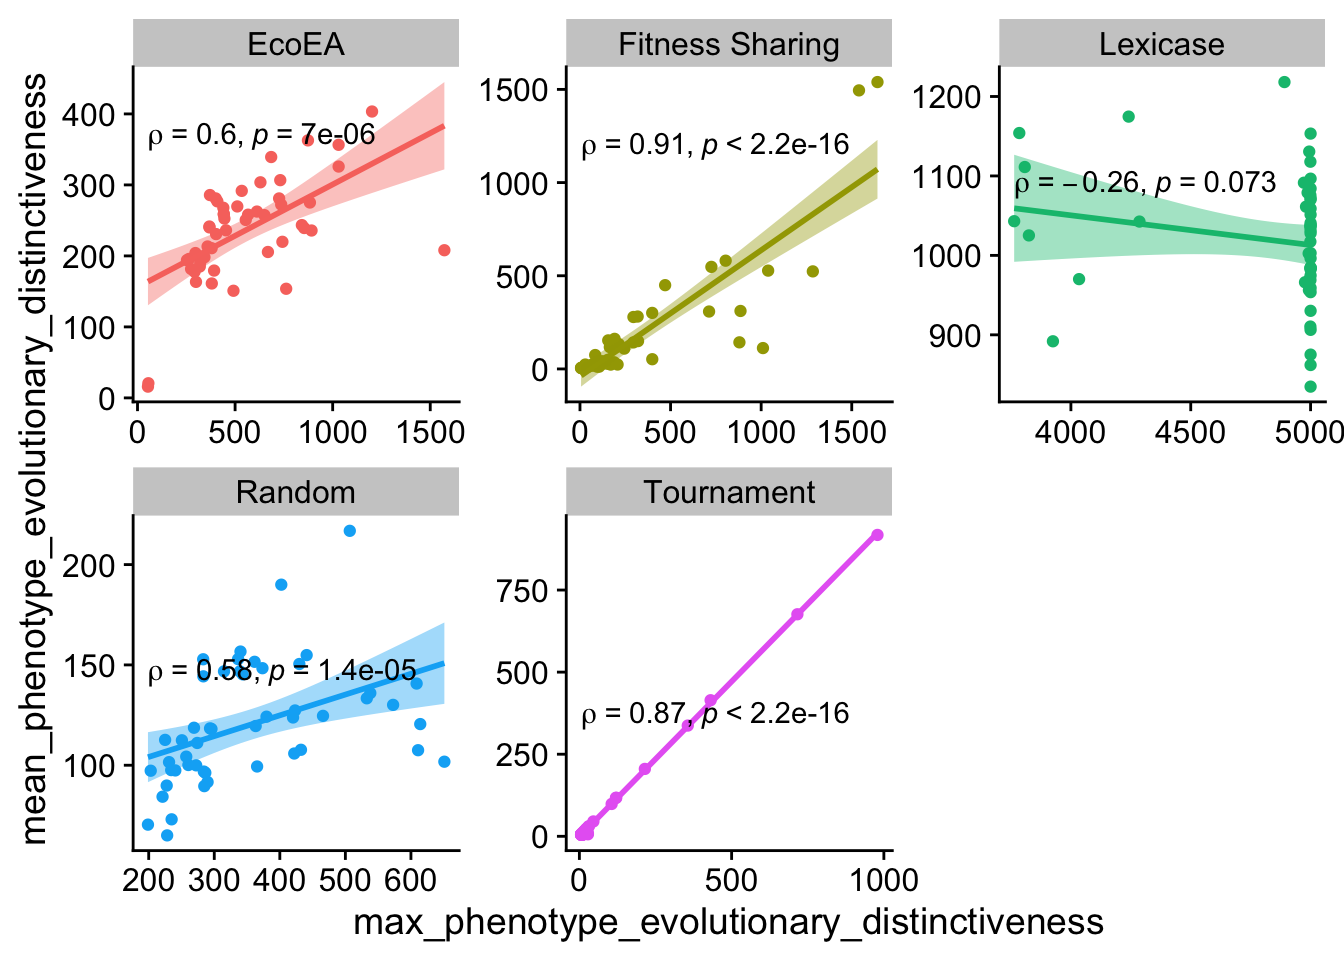
\includegraphics{phylodiversity-in-EC-supplement_files/figure-latex/med_vs_max_ed_early-1.pdf}

And here, for everything except lexicase

\begin{Shaded}
\begin{Highlighting}[]
\KeywordTok{ggplot}\NormalTok{(}
\NormalTok{    data }\OperatorTok\StringTok{ }\KeywordTok{filter}\NormalTok{(gen}\OperatorTok{==}\DecValTok{5000}\NormalTok{),}
    \KeywordTok{aes}\NormalTok{(}
        \DataTypeTok{y=}\NormalTok{mean_phenotype_evolutionary_distinctiveness,}
        \DataTypeTok{x=}\NormalTok{min_phenotype_evolutionary_distinctiveness,}
        \DataTypeTok{color=}\NormalTok{selection_name,}
        \DataTypeTok{fill=}\NormalTok{selection_name}
\NormalTok{    )}
\NormalTok{  ) }\OperatorTok{+}
\StringTok{  }\KeywordTok{geom_point}\NormalTok{() }\OperatorTok{+}
\StringTok{  }\KeywordTok{scale_x_continuous}\NormalTok{(}
        \DataTypeTok{breaks =} \KeywordTok{breaks_extended}\NormalTok{(}\DecValTok{4}\NormalTok{)}
\NormalTok{  ) }\OperatorTok{+}\StringTok{ }
\StringTok{  }\KeywordTok{facet_wrap}\NormalTok{(}
      \OperatorTok{~}\NormalTok{selection_name, }\DataTypeTok{scales=}\StringTok{"free"}
\NormalTok{  ) }\OperatorTok{+}\StringTok{ }
\StringTok{  }\KeywordTok{stat_smooth}\NormalTok{(}
    \DataTypeTok{method=}\StringTok{"lm"}
\NormalTok{  ) }\OperatorTok{+}\StringTok{ }
\StringTok{  }\KeywordTok{stat_cor}\NormalTok{(}
    \DataTypeTok{method=}\StringTok{"spearman"}\NormalTok{, }\DataTypeTok{cor.coef.name =} \StringTok{"rho"}\NormalTok{, }\DataTypeTok{color=}\StringTok{"black"}
\NormalTok{  ) }\OperatorTok{+}
\StringTok{  }\KeywordTok{theme}\NormalTok{(}\DataTypeTok{legend.position =} \StringTok{"none"}\NormalTok{)}
\end{Highlighting}
\end{Shaded}

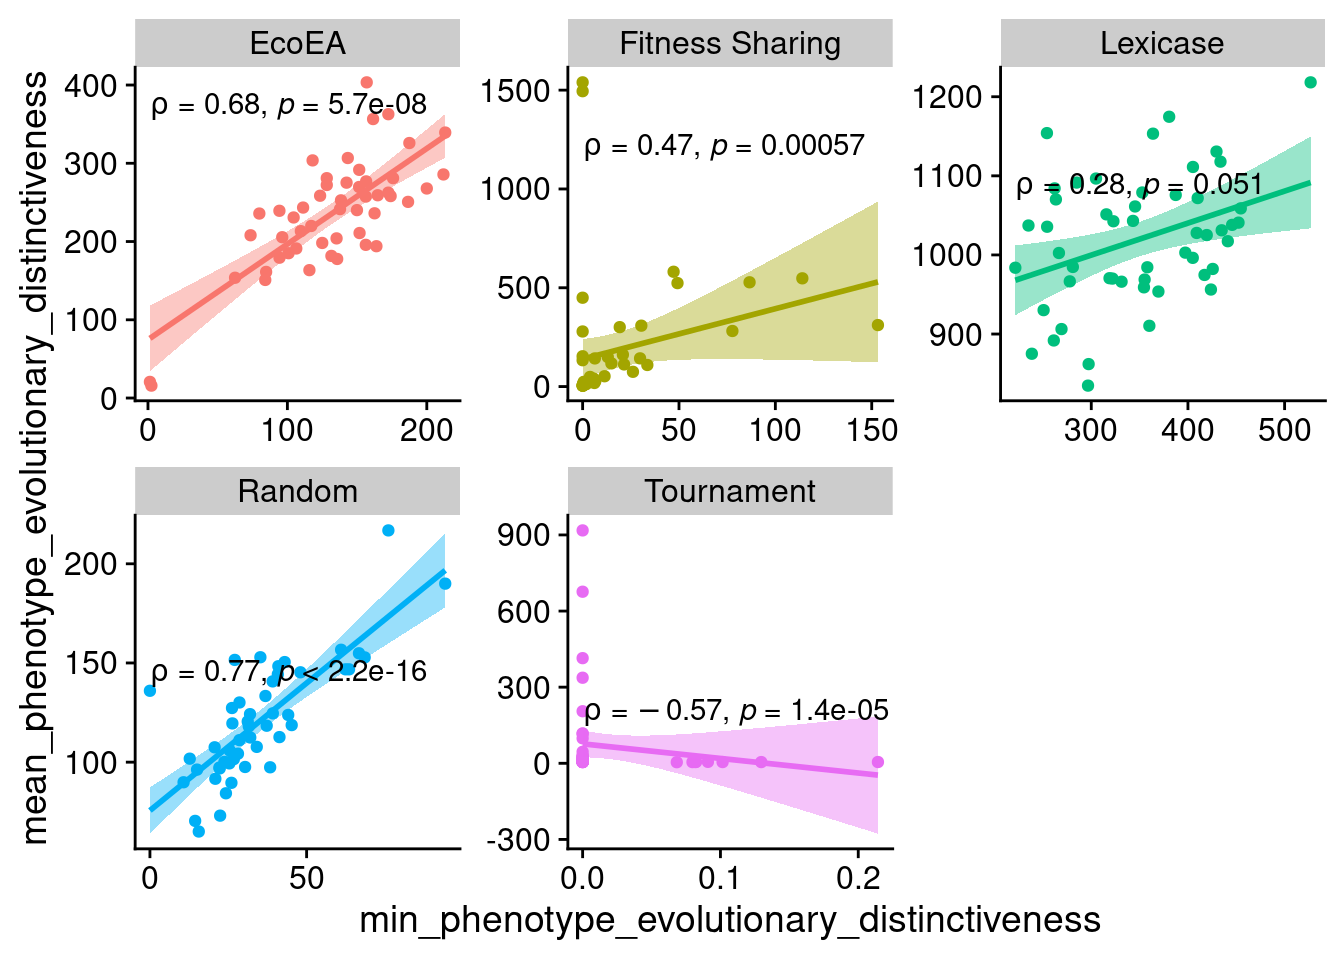
\includegraphics{phylodiversity-in-EC-supplement_files/figure-latex/med_vs_min_ed_early-1.pdf}

These are relatively weak for the most part.

Looks like the evolutionary distinctiveness statistics capture more different information from each other than the pairwise distance statistics (in general the correlations are weaker, and there are more deviations from the pattern of positive correlations). However, in a lot of cases they still correlate. There is definitely more exploration to be done on what differences in these metrics imply, but for simplicity we'll stick to one pairwise distance metric and one evolutionary distinctiveness metric.

Since it's hard to get a gestalt impression from the scatterplots, let's take a look at the correlation matrices for each selection scheme. Note that these are at the final time point, which clearly misses some dynamics that occurr earlier.

\hypertarget{random}{%
\subsubsection{Random}\label{random}}

\begin{Shaded}
\begin{Highlighting}[]
\NormalTok{final_data }\OperatorTok\StringTok{ }
\StringTok{  }\KeywordTok{filter}\NormalTok{(selection_name}\OperatorTok{==}\StringTok{"Random"}\NormalTok{) }\OperatorTok
\StringTok{  }\KeywordTok{transmute}\NormalTok{(}\DataTypeTok{MinPD=}\NormalTok{min_phenotype_pairwise_distance, }
            \DataTypeTok{MeanPD=}\NormalTok{mean_phenotype_pairwise_distance, }
            \DataTypeTok{MaxPD=}\NormalTok{max_phenotype_pairwise_distance, }
            \DataTypeTok{VarPD=}\NormalTok{variance_phenotype_pairwise_distance, }
            \DataTypeTok{MinED =}\NormalTok{ min_phenotype_evolutionary_distinctiveness,}
            \DataTypeTok{MeanED=}\NormalTok{ mean_phenotype_evolutionary_distinctiveness,}
            \DataTypeTok{MaxED=}\NormalTok{max_phenotype_evolutionary_distinctiveness,}
            \DataTypeTok{VarED=}\NormalTok{variance_phenotype_evolutionary_distinctiveness,}
            \DataTypeTok{PD=}\NormalTok{phenotype_current_phylogenetic_diversity,  }\CommentTok{# See Faith 1992}
            \DataTypeTok{MRCA=}\NormalTok{phen_mrca_depth,  }\CommentTok{# Phylogenetic depth of most recent common ancestor}
            \DataTypeTok{N=}\NormalTok{phen_num_taxa     }\CommentTok{# Number of taxonomically-distinct phenotypes}
\NormalTok{  ) }\OperatorTok
\StringTok{  }\KeywordTok{cor_mat}\NormalTok{() }\OperatorTok\StringTok{ }
\StringTok{  }\KeywordTok{pull_lower_triangle}\NormalTok{() }\OperatorTok\StringTok{ }
\StringTok{  }\KeywordTok{cor_plot}\NormalTok{()}
\end{Highlighting}
\end{Shaded}

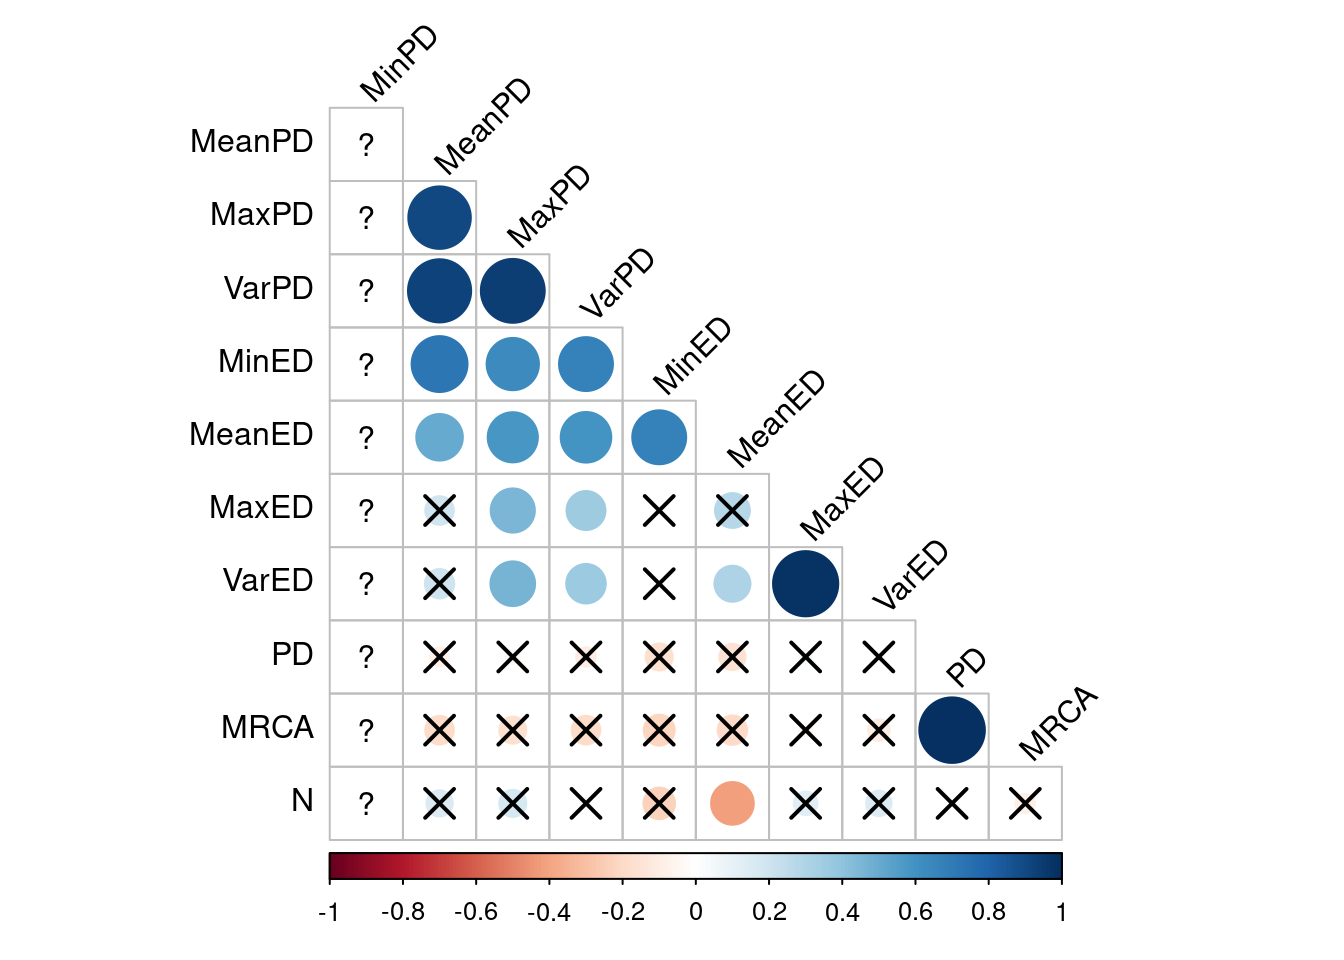
\includegraphics{phylodiversity-in-EC-supplement_files/figure-latex/phylodiversity_correlation_plot_random-1.pdf}

In random selection, all the pairwise distance metrics correlate with each other, and also more weakly with some of the evolutionary distinctiveness metrics, but not max and variance (although they correlate strongly with each other). It is somewhat surprising that the depth of the most recent common ancestor and Faith's Phylogenetic Diveristy metric have so little correlation with the others.

\hypertarget{tournament}{%
\subsubsection{Tournament}\label{tournament}}

\begin{Shaded}
\begin{Highlighting}[]
\NormalTok{final_data }\OperatorTok\StringTok{ }
\StringTok{  }\KeywordTok{filter}\NormalTok{(selection_name}\OperatorTok{==}\StringTok{"Tournament"}\NormalTok{) }\OperatorTok
\StringTok{  }\KeywordTok{transmute}\NormalTok{(}\DataTypeTok{MinPD=}\NormalTok{min_phenotype_pairwise_distance, }
            \DataTypeTok{MeanPD=}\NormalTok{mean_phenotype_pairwise_distance, }
            \DataTypeTok{MaxPD=}\NormalTok{max_phenotype_pairwise_distance, }
            \DataTypeTok{VarPD=}\NormalTok{variance_phenotype_pairwise_distance, }
            \DataTypeTok{MinED =}\NormalTok{ min_phenotype_evolutionary_distinctiveness,}
            \DataTypeTok{MeanED=}\NormalTok{ mean_phenotype_evolutionary_distinctiveness,}
            \DataTypeTok{MaxED=}\NormalTok{max_phenotype_evolutionary_distinctiveness,}
            \DataTypeTok{VarED=}\NormalTok{variance_phenotype_evolutionary_distinctiveness,}
            \DataTypeTok{PD=}\NormalTok{phenotype_current_phylogenetic_diversity,  }\CommentTok{# See Faith 1992}
            \DataTypeTok{MRCA=}\NormalTok{phen_mrca_depth,  }\CommentTok{# Phylogenetic depth of most recent common ancestor}
            \DataTypeTok{N=}\NormalTok{phen_num_taxa     }\CommentTok{# Number of taxonomically-distinct phenotypes}
\NormalTok{  ) }\OperatorTok
\StringTok{  }\KeywordTok{cor_mat}\NormalTok{() }\OperatorTok\StringTok{ }
\StringTok{  }\KeywordTok{pull_lower_triangle}\NormalTok{() }\OperatorTok\StringTok{ }
\StringTok{  }\KeywordTok{cor_plot}\NormalTok{()}
\end{Highlighting}
\end{Shaded}

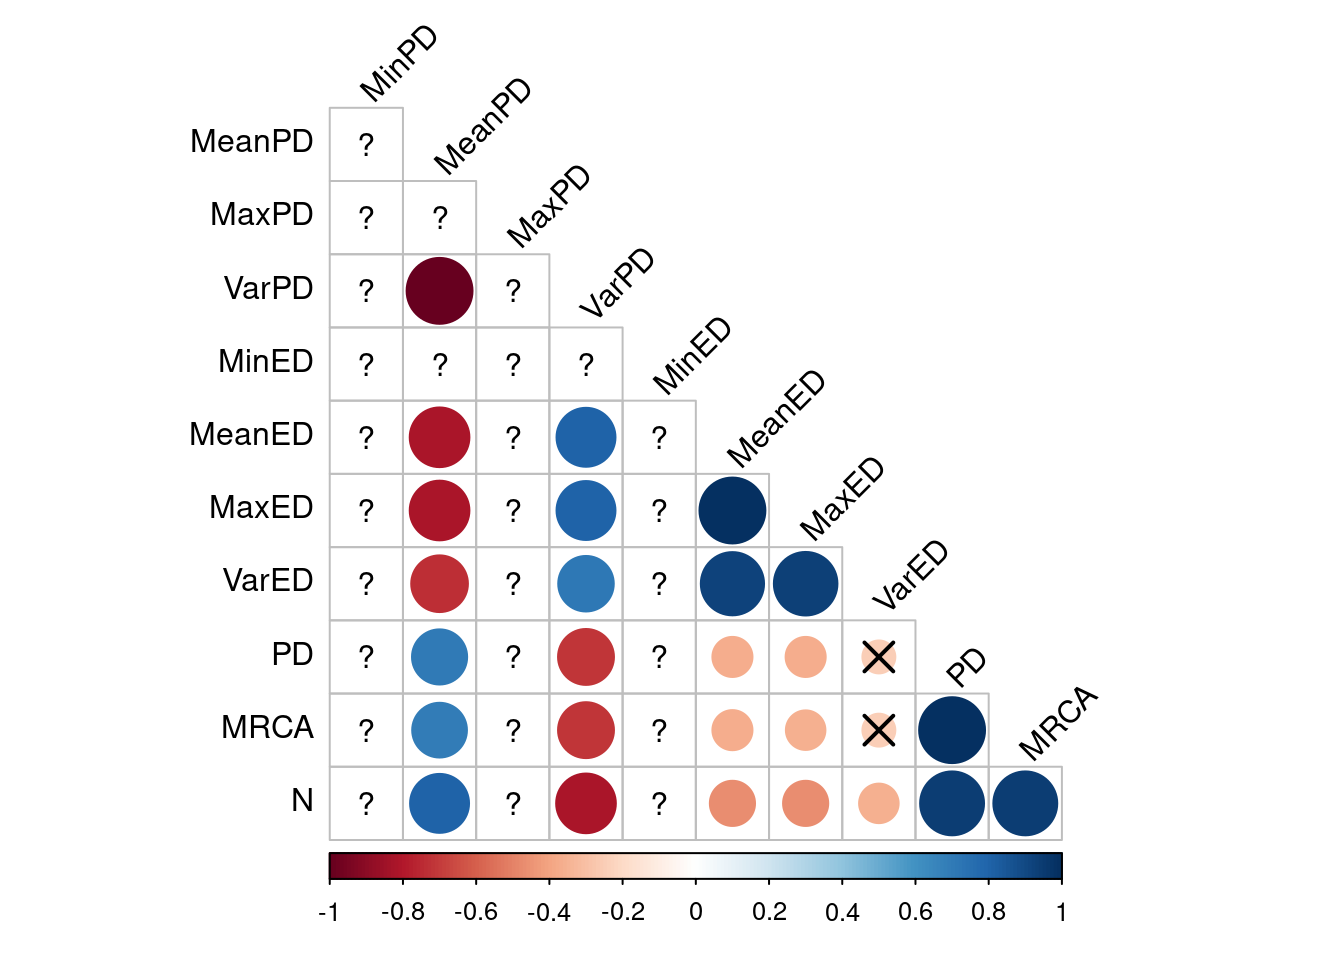
\includegraphics{phylodiversity-in-EC-supplement_files/figure-latex/phylodiversity_correlation_plot_tournament-1.pdf}

Here, all the evolutionary distinctiveness metrics coreelate strongly with each other, but the pairiwse distance metrics less so (although this is likely an artifact of the extremely low phylogenetic diversity in tournament selection)

\hypertarget{fitness-sharing}{%
\subsubsection{Fitness Sharing}\label{fitness-sharing}}

\begin{Shaded}
\begin{Highlighting}[]
\NormalTok{final_data }\OperatorTok\StringTok{ }
\StringTok{  }\KeywordTok{filter}\NormalTok{(selection_name}\OperatorTok{==}\StringTok{"Fitness Sharing"}\NormalTok{) }\OperatorTok
\StringTok{  }\KeywordTok{transmute}\NormalTok{(}\DataTypeTok{MinPD=}\NormalTok{min_phenotype_pairwise_distance, }
            \DataTypeTok{MeanPD=}\NormalTok{mean_phenotype_pairwise_distance, }
            \DataTypeTok{MaxPD=}\NormalTok{max_phenotype_pairwise_distance, }
            \DataTypeTok{VarPD=}\NormalTok{variance_phenotype_pairwise_distance, }
            \DataTypeTok{MinED =}\NormalTok{ min_phenotype_evolutionary_distinctiveness,}
            \DataTypeTok{MeanED=}\NormalTok{ mean_phenotype_evolutionary_distinctiveness,}
            \DataTypeTok{MaxED=}\NormalTok{max_phenotype_evolutionary_distinctiveness,}
            \DataTypeTok{VarED=}\NormalTok{variance_phenotype_evolutionary_distinctiveness,}
            \DataTypeTok{PD=}\NormalTok{phenotype_current_phylogenetic_diversity,  }\CommentTok{# See Faith 1992}
            \DataTypeTok{MRCA=}\NormalTok{phen_mrca_depth,  }\CommentTok{# Phylogenetic depth of most recent common ancestor}
            \DataTypeTok{N=}\NormalTok{phen_num_taxa     }\CommentTok{# Number of taxonomically-distinct phenotypes}
\NormalTok{  ) }\OperatorTok
\StringTok{  }\KeywordTok{cor_mat}\NormalTok{() }\OperatorTok\StringTok{ }
\StringTok{  }\KeywordTok{pull_lower_triangle}\NormalTok{() }\OperatorTok\StringTok{ }
\StringTok{  }\KeywordTok{cor_plot}\NormalTok{()}
\end{Highlighting}
\end{Shaded}

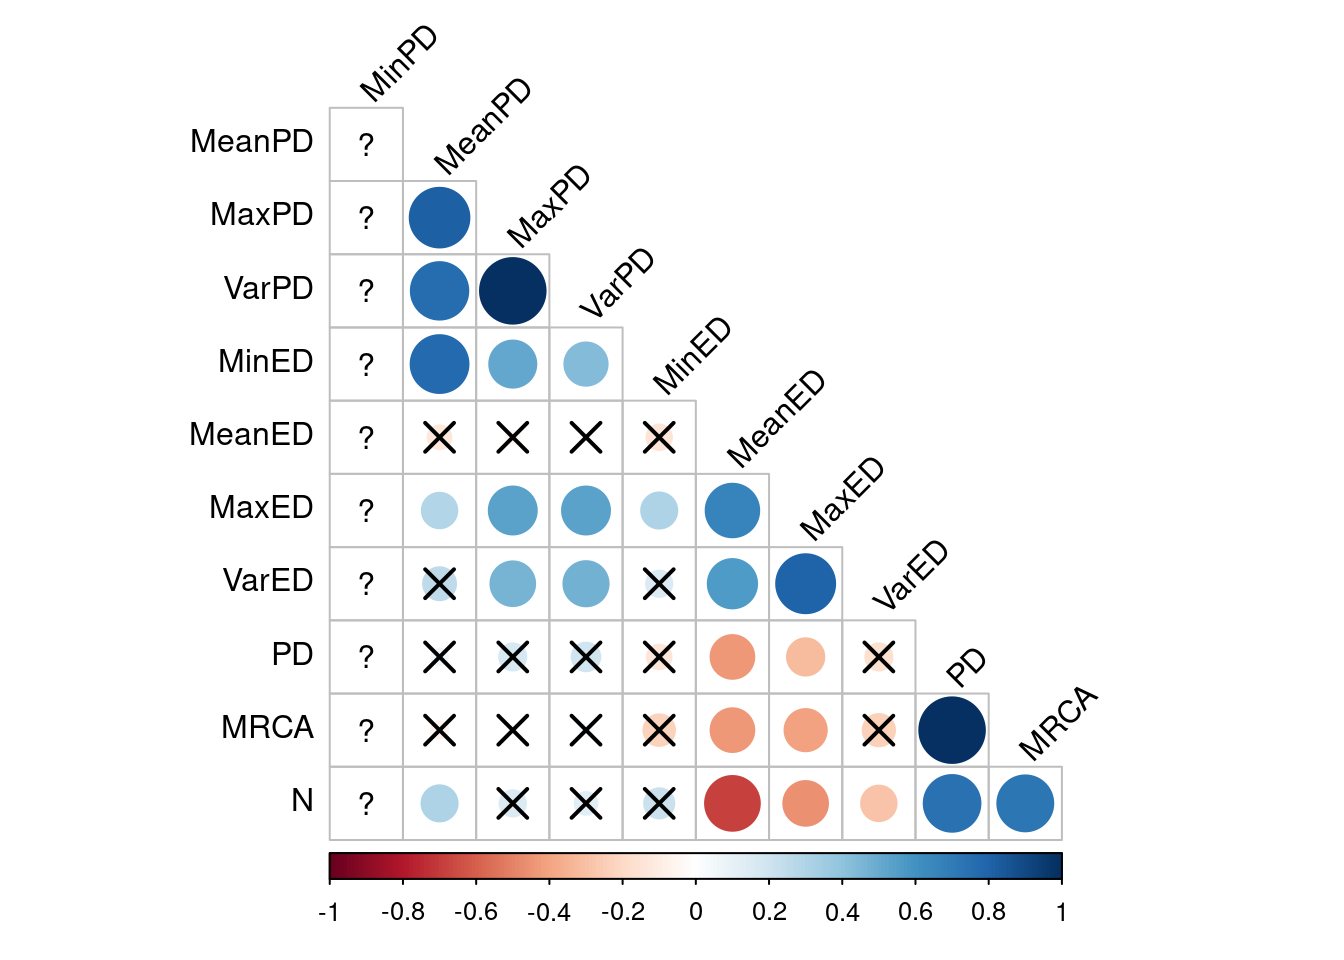
\includegraphics{phylodiversity-in-EC-supplement_files/figure-latex/phylodiversity_correlation_plot_sharing-1.pdf}

Here, the pairwise distance metrics correlate with each other and the evolutionary distinctivenes metrics correlated with each other. There are some correlations between pairwise distance and evolutionary distinctiveness metrics, but they're weaker.

\hypertarget{lexicase-selection}{%
\subsubsection{Lexicase selection}\label{lexicase-selection}}

\begin{Shaded}
\begin{Highlighting}[]
\NormalTok{final_data }\OperatorTok\StringTok{ }
\StringTok{  }\KeywordTok{filter}\NormalTok{(selection_name}\OperatorTok{==}\StringTok{"Lexicase"}\NormalTok{) }\OperatorTok
\StringTok{  }\KeywordTok{transmute}\NormalTok{(}\DataTypeTok{MinPD=}\NormalTok{min_phenotype_pairwise_distance, }
            \DataTypeTok{MeanPD=}\NormalTok{mean_phenotype_pairwise_distance, }
            \DataTypeTok{MaxPD=}\NormalTok{max_phenotype_pairwise_distance, }
            \DataTypeTok{VarPD=}\NormalTok{variance_phenotype_pairwise_distance, }
            \DataTypeTok{MinED =}\NormalTok{ min_phenotype_evolutionary_distinctiveness,}
            \DataTypeTok{MeanED=}\NormalTok{ mean_phenotype_evolutionary_distinctiveness,}
            \DataTypeTok{MaxED=}\NormalTok{max_phenotype_evolutionary_distinctiveness,}
            \DataTypeTok{VarED=}\NormalTok{variance_phenotype_evolutionary_distinctiveness,}
            \DataTypeTok{PD=}\NormalTok{phenotype_current_phylogenetic_diversity,  }\CommentTok{# See Faith 1992}
            \DataTypeTok{MRCA=}\NormalTok{phen_mrca_depth,  }\CommentTok{# Phylogenetic depth of most recent common ancestor}
            \DataTypeTok{N=}\NormalTok{phen_num_taxa     }\CommentTok{# Number of taxonomically-distinct phenotypes}
\NormalTok{  ) }\OperatorTok
\StringTok{  }\KeywordTok{cor_mat}\NormalTok{() }\OperatorTok\StringTok{ }
\StringTok{  }\KeywordTok{pull_lower_triangle}\NormalTok{() }\OperatorTok\StringTok{ }
\StringTok{  }\KeywordTok{cor_plot}\NormalTok{()}
\end{Highlighting}
\end{Shaded}

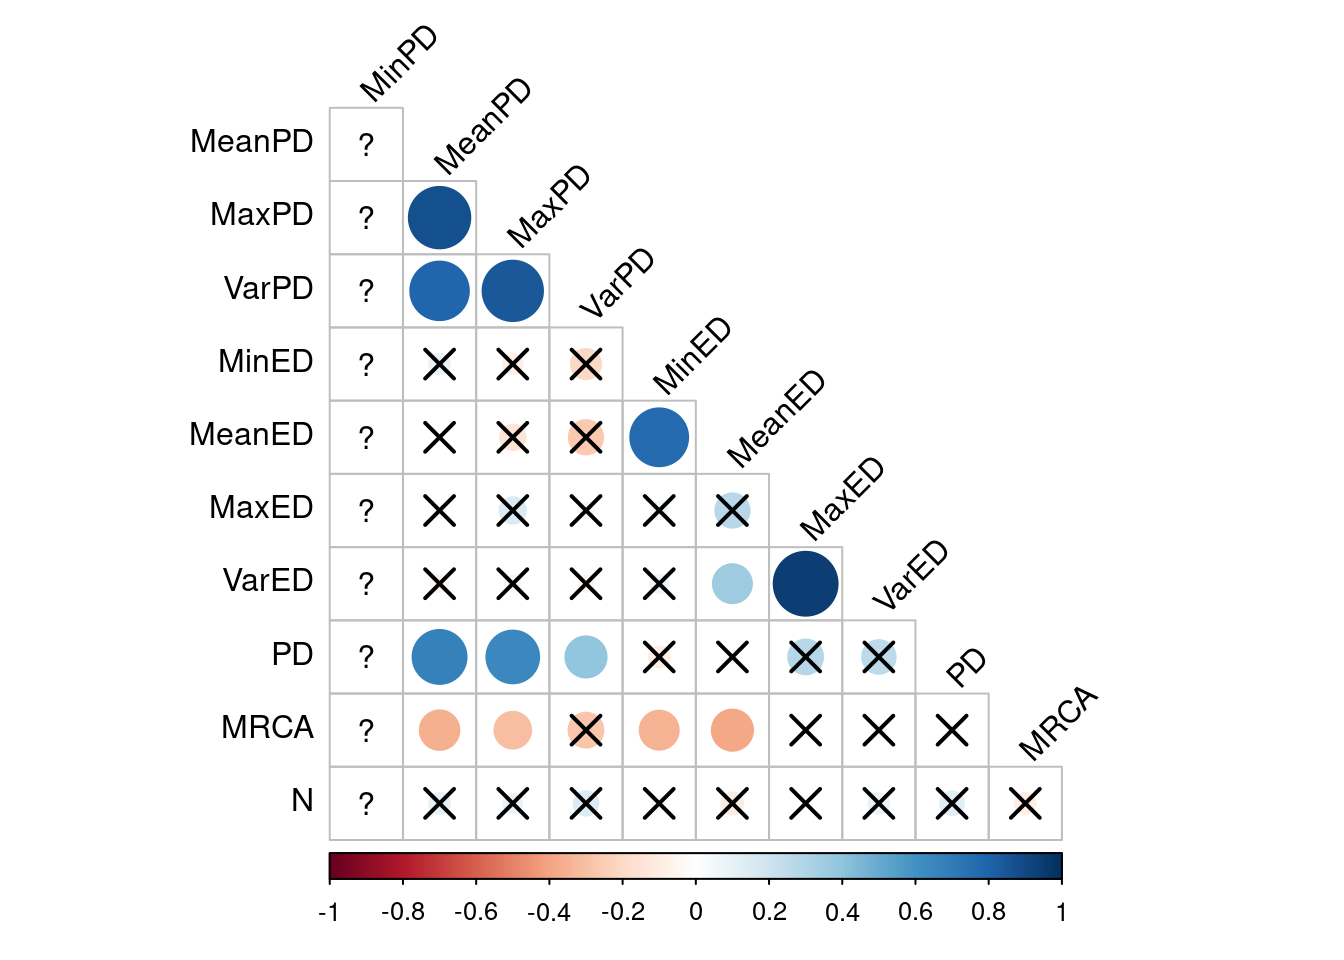
\includegraphics{phylodiversity-in-EC-supplement_files/figure-latex/phylodiversity_correlation_plot_lexicase-1.pdf}

Again, the pairwise distance metrics correlate with each other but not wth the volutionary distinctivness metrics. The evolutionary distinctiveness metrics sort of correlate with each other.

\hypertarget{eco-ea}{%
\subsubsection{Eco-EA}\label{eco-ea}}

\begin{Shaded}
\begin{Highlighting}[]
\NormalTok{final_data }\OperatorTok\StringTok{ }
\StringTok{  }\KeywordTok{filter}\NormalTok{(selection_name}\OperatorTok{==}\StringTok{"EcoEA"}\NormalTok{) }\OperatorTok
\StringTok{  }\KeywordTok{transmute}\NormalTok{(}\DataTypeTok{MinPD=}\NormalTok{min_phenotype_pairwise_distance, }
            \DataTypeTok{MeanPD=}\NormalTok{mean_phenotype_pairwise_distance, }
            \DataTypeTok{MaxPD=}\NormalTok{max_phenotype_pairwise_distance, }
            \DataTypeTok{VarPD=}\NormalTok{variance_phenotype_pairwise_distance, }
            \DataTypeTok{MinED =}\NormalTok{ min_phenotype_evolutionary_distinctiveness,}
            \DataTypeTok{MeanED=}\NormalTok{ mean_phenotype_evolutionary_distinctiveness,}
            \DataTypeTok{MaxED=}\NormalTok{max_phenotype_evolutionary_distinctiveness,}
            \DataTypeTok{VarED=}\NormalTok{variance_phenotype_evolutionary_distinctiveness,}
            \DataTypeTok{PD=}\NormalTok{phenotype_current_phylogenetic_diversity,  }\CommentTok{# See Faith 1992}
            \DataTypeTok{MRCA=}\NormalTok{phen_mrca_depth,  }\CommentTok{# Phylogenetic depth of most recent common ancestor}
            \DataTypeTok{N=}\NormalTok{phen_num_taxa     }\CommentTok{# Number of taxonomically-distinct phenotypes}
\NormalTok{  ) }\OperatorTok
\StringTok{  }\KeywordTok{cor_mat}\NormalTok{() }\OperatorTok\StringTok{ }
\StringTok{  }\KeywordTok{pull_lower_triangle}\NormalTok{() }\OperatorTok\StringTok{ }
\StringTok{  }\KeywordTok{cor_plot}\NormalTok{()}
\end{Highlighting}
\end{Shaded}

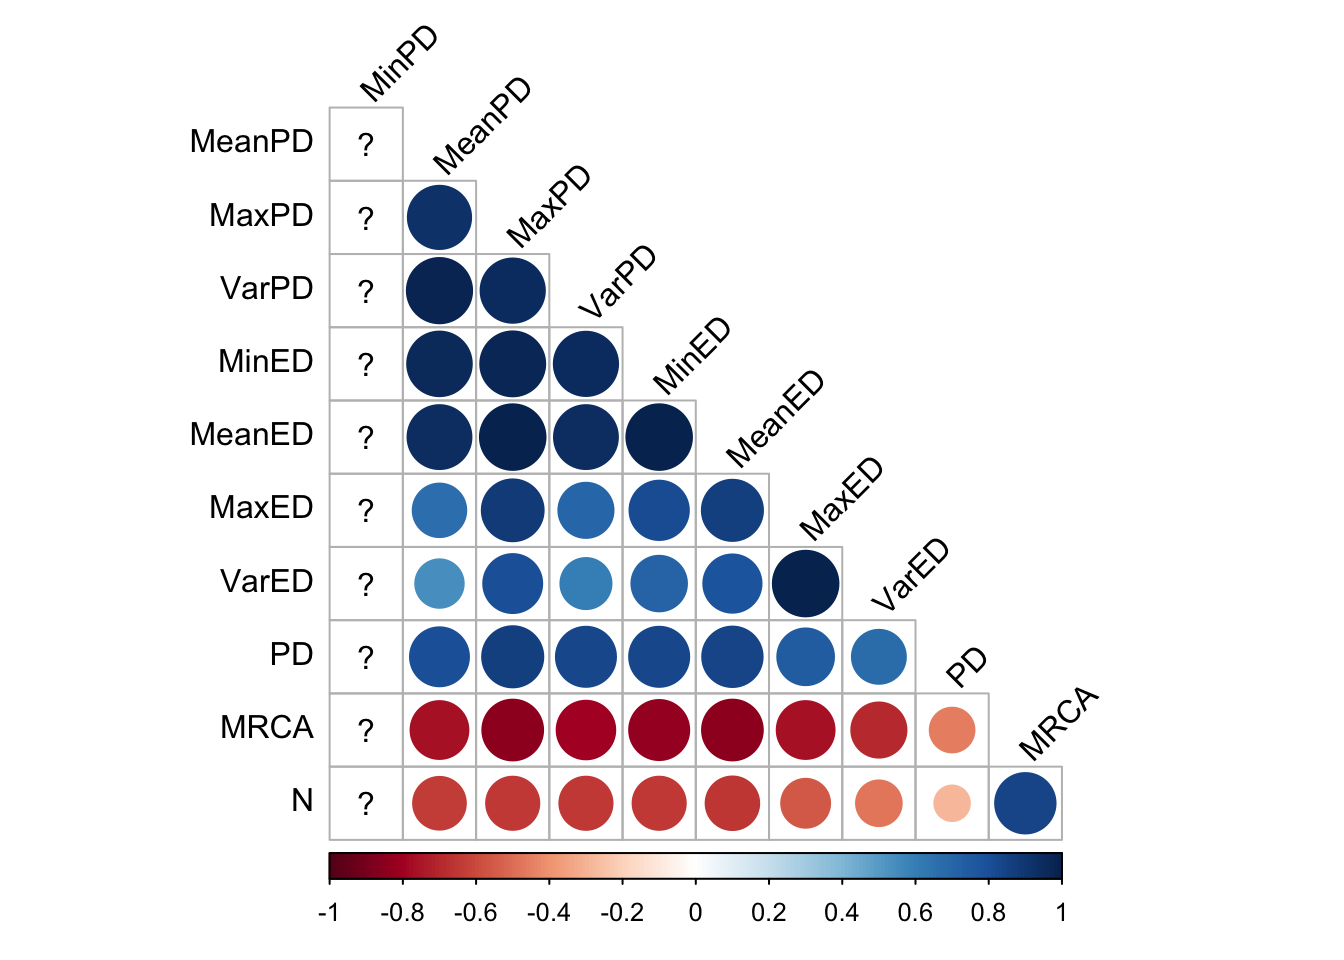
\includegraphics{phylodiversity-in-EC-supplement_files/figure-latex/phylodiversity_correlation_plot_ecoea-1.pdf}

In Eco-EA, there is an impressively strong positive correlation among all the phylodiversity metrics. Understanding what causes Eco-EA to deviate from lexicase selection (and to a lesser extent fitness sharing) in this way would be worthy of further research.

\hypertarget{over-time-1}{%
\subsection{Over time}\label{over-time-1}}

\hypertarget{mean-pairwise-distance}{%
\subsubsection{Mean pairwise distance}\label{mean-pairwise-distance}}

First we plot mean pairwise distance over time. We log the y axis because there is such variation in mean pairwise distance across selection schemes, and the x-axis for the same reason as before.

\begin{Shaded}
\begin{Highlighting}[]
\KeywordTok{ggplot}\NormalTok{(}
\NormalTok{    data,}
    \KeywordTok{aes}\NormalTok{(}
      \DataTypeTok{x=}\NormalTok{gen,}
      \DataTypeTok{y=}\NormalTok{mean_phenotype_pairwise_distance,}
      \DataTypeTok{color=}\NormalTok{selection_name,}
      \DataTypeTok{fill=}\NormalTok{selection_name}
\NormalTok{    )}
\NormalTok{  ) }\OperatorTok{+}
\StringTok{  }\KeywordTok{stat_summary}\NormalTok{(}\DataTypeTok{geom=}\StringTok{"line"}\NormalTok{, }\DataTypeTok{fun=}\NormalTok{mean) }\OperatorTok{+}
\StringTok{  }\KeywordTok{stat_summary}\NormalTok{(}
    \DataTypeTok{geom=}\StringTok{"ribbon"}\NormalTok{,}
    \DataTypeTok{fun.data=}\StringTok{"mean_cl_boot"}\NormalTok{,}
    \DataTypeTok{fun.args=}\KeywordTok{list}\NormalTok{(}\DataTypeTok{conf.int=}\FloatTok{0.95}\NormalTok{),}
    \DataTypeTok{alpha=}\FloatTok{0.2}\NormalTok{,}
    \DataTypeTok{linetype=}\DecValTok{0}
\NormalTok{  ) }\OperatorTok{+}
\StringTok{  }\KeywordTok{scale_y_log10}\NormalTok{(}
    \DataTypeTok{name=}\StringTok{"Mean pairwise distance"}
\NormalTok{  ) }\OperatorTok{+}
\StringTok{  }\KeywordTok{scale_x_log10}\NormalTok{(}
    \DataTypeTok{name=}\StringTok{"Generation"}
\NormalTok{  ) }\OperatorTok{+}
\StringTok{  }\KeywordTok{scale_color_discrete}\NormalTok{(}\StringTok{"Selection"}\NormalTok{) }\OperatorTok{+}
\StringTok{  }\KeywordTok{scale_fill_discrete}\NormalTok{(}\StringTok{"Selection"}\NormalTok{)}
\end{Highlighting}
\end{Shaded}

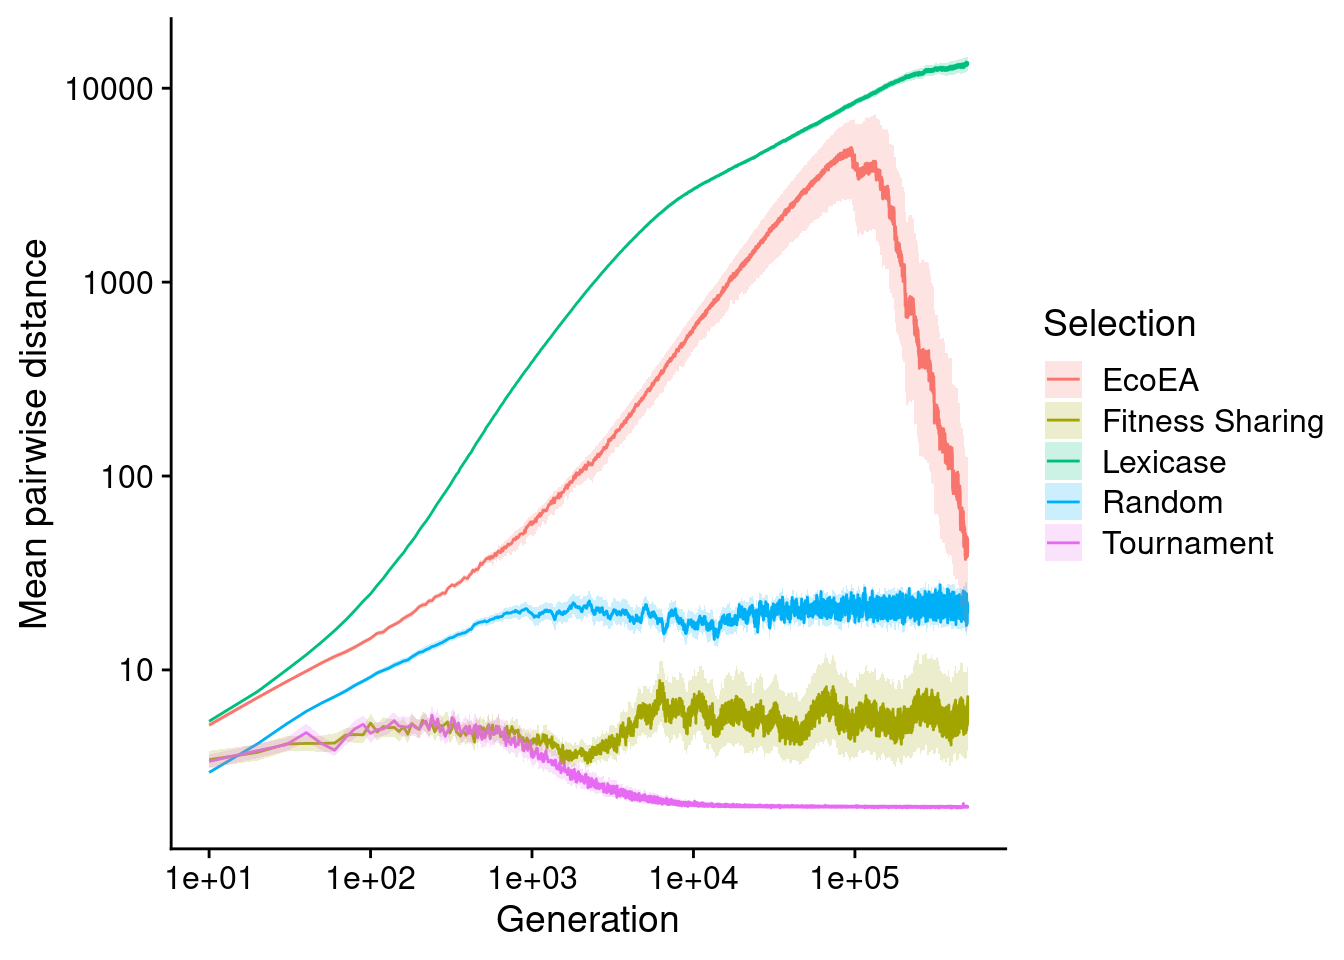
\includegraphics{phylodiversity-in-EC-supplement_files/figure-latex/phylogeny_over_time_plot_mpd-1.pdf}

Lexicase selection maintains a monotonic increase in phylogenetic diversity over the course of the entire experiment. It likely never experiences a full coalescence event (where the most-recent common ancestor changes). Eco-EA nearly keeps pace with lexicase selection until towards the end, when its phylogenetic diversity crashes. This is likely the result of selective sweeps that begin to occur as the population discovers high fitness solutions. Fitness sharing shows a slight dip at the same time that its fitness plateaus (likely also the result of a selective sweep), but phylogenetic diversity recovers afterwards, making for a relatively constant level. over time. Tournament selection, on the other hand, maintains the same (low) level of phylogenetic diversity as fitness sharing, up until the point that fitness plateaus, at which point tournament selection's phylodiversity drops to nearly 0. Interestingly, lexicase selection and Eco-EA both maintain more phylodiversity than random selection, whereas fitness sharing and tournament selection maintain less.

\hypertarget{mean-evolutionary-distinctiveness}{%
\subsubsection{Mean evolutionary distinctiveness}\label{mean-evolutionary-distinctiveness}}

For comparison, we make the same plot with mean evolutionary distinctiveness.

\begin{Shaded}
\begin{Highlighting}[]
\KeywordTok{ggplot}\NormalTok{(}
\NormalTok{    data,}
    \KeywordTok{aes}\NormalTok{(}
      \DataTypeTok{x=}\NormalTok{gen,}
      \DataTypeTok{y=}\NormalTok{mean_phenotype_evolutionary_distinctiveness,}
      \DataTypeTok{color=}\NormalTok{selection_name,}
      \DataTypeTok{fill=}\NormalTok{selection_name}
\NormalTok{    )}
\NormalTok{  ) }\OperatorTok{+}
\StringTok{  }\KeywordTok{stat_summary}\NormalTok{(}\DataTypeTok{geom=}\StringTok{"line"}\NormalTok{, }\DataTypeTok{fun=}\NormalTok{mean) }\OperatorTok{+}
\StringTok{  }\KeywordTok{stat_summary}\NormalTok{(}
    \DataTypeTok{geom=}\StringTok{"ribbon"}\NormalTok{,}
    \DataTypeTok{fun.data=}\StringTok{"mean_cl_boot"}\NormalTok{,}
    \DataTypeTok{fun.args=}\KeywordTok{list}\NormalTok{(}\DataTypeTok{conf.int=}\FloatTok{0.95}\NormalTok{),}
    \DataTypeTok{alpha=}\FloatTok{0.2}\NormalTok{,}
    \DataTypeTok{linetype=}\DecValTok{0}
\NormalTok{  ) }\OperatorTok{+}
\StringTok{  }\KeywordTok{scale_y_log10}\NormalTok{(}
    \DataTypeTok{name=}\StringTok{"Mean evolutionary distinctiveness"}
\NormalTok{  ) }\OperatorTok{+}
\StringTok{  }\KeywordTok{scale_x_log10}\NormalTok{(}
    \DataTypeTok{name=}\StringTok{"Generation"}
\NormalTok{  ) }\OperatorTok{+}
\StringTok{  }\KeywordTok{scale_color_discrete}\NormalTok{(}\StringTok{"Selection"}\NormalTok{) }\OperatorTok{+}
\StringTok{  }\KeywordTok{scale_fill_discrete}\NormalTok{(}\StringTok{"Selection"}\NormalTok{)}
\end{Highlighting}
\end{Shaded}

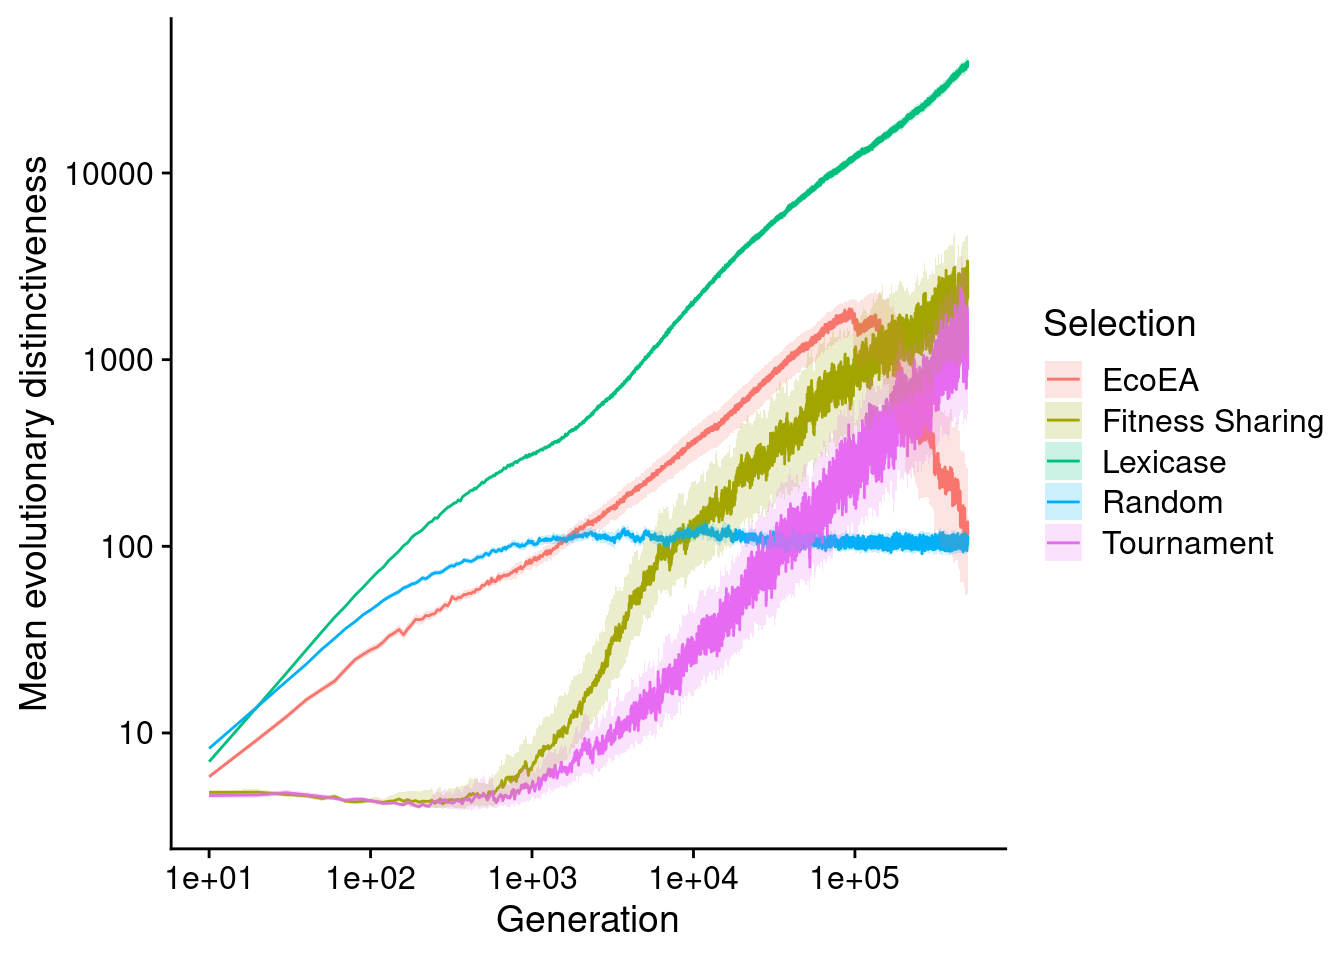
\includegraphics{phylodiversity-in-EC-supplement_files/figure-latex/phylogeny_over_time_plot_med-1.pdf}

Interestingly, Fitness Sharing and tournament selection both start increasing in evolutionary distinctiveness only after their fitnesses have plateaued. This seems likely to be due to some sort of pathological behavior of mean evolutionary distinctiveness on small trees, but more investigation would be necessary to figure out exactly what's going on. Trends in other selection schemes are largely similar.

\hypertarget{final-1}{%
\subsection{Final}\label{final-1}}

Next, we perform a more in-depth analysis of phylodiversity distributions at the final time point.

\hypertarget{mean-pairwise-distance-1}{%
\subsubsection{Mean pairwise distance}\label{mean-pairwise-distance-1}}

First, we test which selection schemes end up with significantly different final distributions of mean pairwise distance.

\begin{Shaded}
\begin{Highlighting}[]
\CommentTok{# Pairwise wilcoxon teset to determine which conditions are significantly different from each other}
\NormalTok{stat.test <-}\StringTok{ }\NormalTok{final_data }\OperatorTok
\StringTok{  }\KeywordTok{wilcox_test}\NormalTok{(mean_phenotype_pairwise_distance }\OperatorTok{~}\StringTok{ }\NormalTok{selection_name) }\OperatorTok
\StringTok{  }\KeywordTok{adjust_pvalue}\NormalTok{(}\DataTypeTok{method =} \StringTok{"bonferroni"}\NormalTok{) }\OperatorTok
\StringTok{  }\KeywordTok{add_significance}\NormalTok{() }\OperatorTok
\StringTok{  }\KeywordTok{add_xy_position}\NormalTok{(}\DataTypeTok{x=}\StringTok{"selection_name"}\NormalTok{,}\DataTypeTok{step.increase=}\DecValTok{1}\NormalTok{)}
\NormalTok{stat.test}\OperatorTok{$}\NormalTok{label <-}\StringTok{ }\KeywordTok{mapply}\NormalTok{(p_label,stat.test}\OperatorTok{$}\NormalTok{p.adj)}

\CommentTok{# Output stats}
\NormalTok{stat.test }\OperatorTok
\StringTok{  }\KeywordTok{kbl}\NormalTok{() }\OperatorTok
\StringTok{  }\KeywordTok{kable_styling}\NormalTok{(}
    \DataTypeTok{bootstrap_options =} \KeywordTok{c}\NormalTok{(}
      \StringTok{"striped"}\NormalTok{,}
      \StringTok{"hover"}\NormalTok{,}
      \StringTok{"condensed"}\NormalTok{,}
      \StringTok{"responsive"}
\NormalTok{    )}
\NormalTok{  ) }\OperatorTok
\StringTok{  }\KeywordTok{scroll_box}\NormalTok{(}\DataTypeTok{width=}\StringTok{"600px"}\NormalTok{)}
\end{Highlighting}
\end{Shaded}

\begin{table}
\centering
\begin{tabular}[t]{l|l|l|r|r|r|r|r|l|r|l|r|r|l}
\hline
.y. & group1 & group2 & n1 & n2 & statistic & p & p.adj & p.adj.signif & y.position & groups & xmin & xmax & label\\
\hline
mean\_phenotype\_pairwise\_distance & EcoEA & Fitness Sharing & 50 & 50 & 1824.0 & 7.70e-05 & 7.70e-04 & *** & 49488.81 & EcoEA          , Fitness Sharing & 1 & 2 & p = 0.00077\\
\hline
mean\_phenotype\_pairwise\_distance & EcoEA & Lexicase & 50 & 47 & 227.0 & 0.00e+00 & 0.00e+00 & **** & 76981.49 & EcoEA   , Lexicase & 1 & 3 & p < 1e-04\\
\hline
mean\_phenotype\_pairwise\_distance & EcoEA & Random & 50 & 50 & 690.0 & 1.15e-04 & 1.15e-03 & ** & 104474.18 & EcoEA , Random & 1 & 4 & p = 0.00115\\
\hline
mean\_phenotype\_pairwise\_distance & EcoEA & Tournament & 50 & 50 & 2500.0 & 0.00e+00 & 0.00e+00 & **** & 131966.86 & EcoEA     , Tournament & 1 & 5 & p < 1e-04\\
\hline
mean\_phenotype\_pairwise\_distance & Fitness Sharing & Lexicase & 50 & 47 & 0.0 & 0.00e+00 & 0.00e+00 & **** & 159459.54 & Fitness Sharing, Lexicase & 2 & 3 & p < 1e-04\\
\hline
mean\_phenotype\_pairwise\_distance & Fitness Sharing & Random & 50 & 50 & 536.0 & 9.00e-07 & 8.70e-06 & **** & 186952.22 & Fitness Sharing, Random & 2 & 4 & p < 1e-04\\
\hline
mean\_phenotype\_pairwise\_distance & Fitness Sharing & Tournament & 50 & 50 & 2232.5 & 0.00e+00 & 0.00e+00 & **** & 214444.90 & Fitness Sharing, Tournament & 2 & 5 & p < 1e-04\\
\hline
mean\_phenotype\_pairwise\_distance & Lexicase & Random & 47 & 50 & 2350.0 & 0.00e+00 & 0.00e+00 & **** & 241937.58 & Lexicase, Random & 3 & 4 & p < 1e-04\\
\hline
mean\_phenotype\_pairwise\_distance & Lexicase & Tournament & 47 & 50 & 2350.0 & 0.00e+00 & 0.00e+00 & **** & 269430.26 & Lexicase  , Tournament & 3 & 5 & p < 1e-04\\
\hline
mean\_phenotype\_pairwise\_distance & Random & Tournament & 50 & 50 & 2500.0 & 0.00e+00 & 0.00e+00 & **** & 296922.94 & Random    , Tournament & 4 & 5 & p < 1e-04\\
\hline
\end{tabular}
\end{table}

Looks like they are all significantly different from each other.

\begin{Shaded}
\begin{Highlighting}[]
\CommentTok{# Raincloud plot of final mean pairwise distance}
\NormalTok{final_phylogeny_fig <-}\StringTok{ }\KeywordTok{ggplot}\NormalTok{(}
\NormalTok{    final_data,}
    \KeywordTok{aes}\NormalTok{(}
      \DataTypeTok{x=}\NormalTok{selection_name,}
      \DataTypeTok{y=}\NormalTok{mean_phenotype_pairwise_distance,}
      \DataTypeTok{fill=}\NormalTok{selection_name}
\NormalTok{    )}
\NormalTok{  ) }\OperatorTok{+}
\StringTok{  }\KeywordTok{geom_flat_violin}\NormalTok{(}
    \DataTypeTok{position =} \KeywordTok{position_nudge}\NormalTok{(}\DataTypeTok{x =} \FloatTok{.2}\NormalTok{, }\DataTypeTok{y =} \DecValTok{0}\NormalTok{),}
    \DataTypeTok{alpha =} \FloatTok{.8}\NormalTok{,}
    \DataTypeTok{scale=}\StringTok{"width"}
\NormalTok{  ) }\OperatorTok{+}
\StringTok{  }\KeywordTok{geom_point}\NormalTok{(}
    \DataTypeTok{mapping=}\KeywordTok{aes}\NormalTok{(}\DataTypeTok{color=}\NormalTok{selection_name),}
    \DataTypeTok{position =} \KeywordTok{position_jitter}\NormalTok{(}\DataTypeTok{width =} \FloatTok{.15}\NormalTok{),}
    \DataTypeTok{size =} \FloatTok{.5}\NormalTok{,}
    \DataTypeTok{alpha =} \FloatTok{0.8}
\NormalTok{  ) }\OperatorTok{+}
\StringTok{  }\KeywordTok{geom_boxplot}\NormalTok{(}
    \DataTypeTok{width =} \FloatTok{.1}\NormalTok{,}
    \DataTypeTok{outlier.shape =} \OtherTok{NA}\NormalTok{,}
    \DataTypeTok{alpha =} \FloatTok{0.5}
\NormalTok{  ) }\OperatorTok{+}
\StringTok{  }\KeywordTok{scale_y_log10}\NormalTok{(}
    \DataTypeTok{name=}\StringTok{"Mean pairwise distance"}
\NormalTok{  ) }\OperatorTok{+}
\StringTok{  }\KeywordTok{scale_x_discrete}\NormalTok{(}
    \DataTypeTok{name=}\StringTok{"Selection"}
\NormalTok{  ) }\OperatorTok{+}
\StringTok{  }\KeywordTok{scale_fill_discrete}\NormalTok{(}
    \DataTypeTok{name=}\StringTok{"Selection"}
\NormalTok{  ) }\OperatorTok{+}
\StringTok{  }\KeywordTok{scale_color_discrete}\NormalTok{(}
    \DataTypeTok{name=}\StringTok{"Selection"}
\NormalTok{  ) }\OperatorTok{+}\StringTok{ }
\StringTok{  }\KeywordTok{theme}\NormalTok{(}\DataTypeTok{legend.position =} \StringTok{"none"}\NormalTok{)}
\NormalTok{final_phylogeny_fig}
\end{Highlighting}
\end{Shaded}

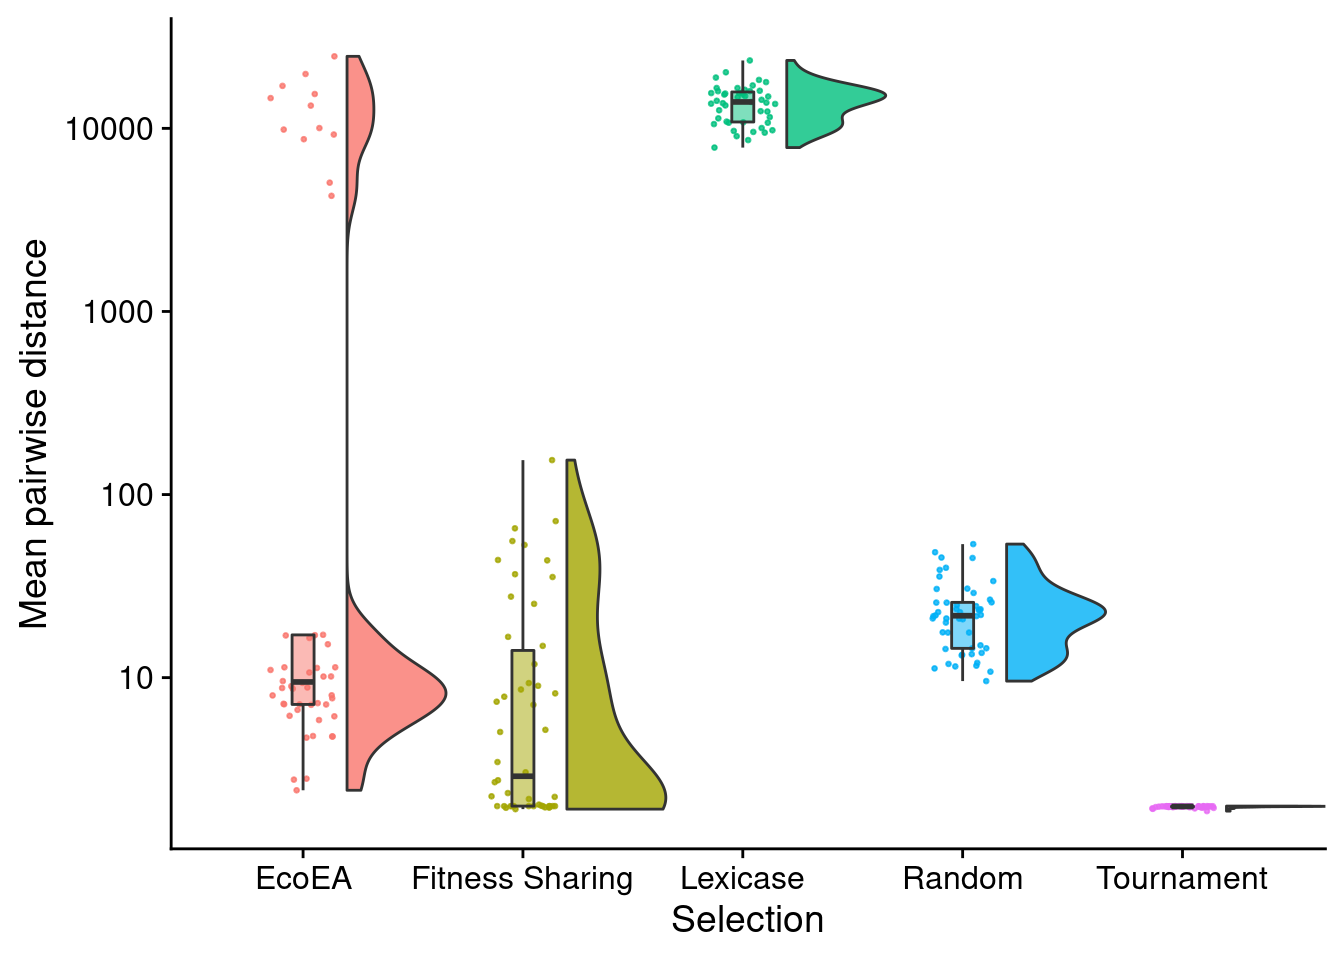
\includegraphics{phylodiversity-in-EC-supplement_files/figure-latex/final_phylogeny_plot_mpd-1.pdf}

This shows something interesting! Final phylogenetic diversity in Eco-EA is heavily bimodal. In later analysis, we will see that the runs with high phylogenetic diversity are the ones with lower fitness, suggesting that they have no yet experienced a selective sweep resulting from the discovery of a high-fitness solution.

\hypertarget{mean-evolutionary-distinctiveness-1}{%
\subsubsection{Mean evolutionary distinctiveness}\label{mean-evolutionary-distinctiveness-1}}

Tests for significant differences:

\begin{Shaded}
\begin{Highlighting}[]
\CommentTok{# Pairwise wilcoxon teset to determine which conditions are significantly different from each other}
\NormalTok{stat.test <-}\StringTok{ }\NormalTok{final_data }\OperatorTok
\StringTok{  }\KeywordTok{wilcox_test}\NormalTok{(mean_phenotype_evolutionary_distinctiveness }\OperatorTok{~}\StringTok{ }\NormalTok{selection_name) }\OperatorTok
\StringTok{  }\KeywordTok{adjust_pvalue}\NormalTok{(}\DataTypeTok{method =} \StringTok{"bonferroni"}\NormalTok{) }\OperatorTok
\StringTok{  }\KeywordTok{add_significance}\NormalTok{() }\OperatorTok
\StringTok{  }\KeywordTok{add_xy_position}\NormalTok{(}\DataTypeTok{x=}\StringTok{"selection_name"}\NormalTok{,}\DataTypeTok{step.increase=}\DecValTok{1}\NormalTok{)}
\NormalTok{stat.test}\OperatorTok{$}\NormalTok{label <-}\StringTok{ }\KeywordTok{mapply}\NormalTok{(p_label,stat.test}\OperatorTok{$}\NormalTok{p.adj)}

\CommentTok{# Output stats}

\NormalTok{stat.test }\OperatorTok
\StringTok{  }\KeywordTok{kbl}\NormalTok{() }\OperatorTok
\StringTok{  }\KeywordTok{kable_styling}\NormalTok{(}
    \DataTypeTok{bootstrap_options =} \KeywordTok{c}\NormalTok{(}
      \StringTok{"striped"}\NormalTok{,}
      \StringTok{"hover"}\NormalTok{,}
      \StringTok{"condensed"}\NormalTok{,}
      \StringTok{"responsive"}
\NormalTok{    )}
\NormalTok{  ) }\OperatorTok
\StringTok{  }\KeywordTok{scroll_box}\NormalTok{(}\DataTypeTok{width=}\StringTok{"600px"}\NormalTok{)}
\end{Highlighting}
\end{Shaded}

\begin{table}
\centering
\begin{tabular}[t]{l|l|l|r|r|r|r|r|l|r|l|r|r|l}
\hline
.y. & group1 & group2 & n1 & n2 & statistic & p & p.adj & p.adj.signif & y.position & groups & xmin & xmax & label\\
\hline
mean\_phenotype\_evolutionary\_distinctiveness & EcoEA & Fitness Sharing & 50 & 50 & 469 & 1.00e-07 & 7.00e-07 & **** & 289111.7 & EcoEA          , Fitness Sharing & 1 & 2 & p < 1e-04\\
\hline
mean\_phenotype\_evolutionary\_distinctiveness & EcoEA & Lexicase & 50 & 47 & 0 & 0.00e+00 & 0.00e+00 & **** & 449625.8 & EcoEA   , Lexicase & 1 & 3 & p < 1e-04\\
\hline
mean\_phenotype\_evolutionary\_distinctiveness & EcoEA & Random & 50 & 50 & 711 & 2.05e-04 & 2.05e-03 & ** & 610140.0 & EcoEA , Random & 1 & 4 & p = 0.00205\\
\hline
mean\_phenotype\_evolutionary\_distinctiveness & EcoEA & Tournament & 50 & 50 & 569 & 2.70e-06 & 2.72e-05 & **** & 770654.1 & EcoEA     , Tournament & 1 & 5 & p < 1e-04\\
\hline
mean\_phenotype\_evolutionary\_distinctiveness & Fitness Sharing & Lexicase & 50 & 47 & 100 & 0.00e+00 & 0.00e+00 & **** & 931168.2 & Fitness Sharing, Lexicase & 2 & 3 & p < 1e-04\\
\hline
mean\_phenotype\_evolutionary\_distinctiveness & Fitness Sharing & Random & 50 & 50 & 2428 & 0.00e+00 & 0.00e+00 & **** & 1091682.4 & Fitness Sharing, Random & 2 & 4 & p < 1e-04\\
\hline
mean\_phenotype\_evolutionary\_distinctiveness & Fitness Sharing & Tournament & 50 & 50 & 1614 & 1.20e-02 & 1.20e-01 & ns & 1252196.5 & Fitness Sharing, Tournament & 2 & 5 & p = 0.12\\
\hline
mean\_phenotype\_evolutionary\_distinctiveness & Lexicase & Random & 47 & 50 & 2350 & 0.00e+00 & 0.00e+00 & **** & 1412710.6 & Lexicase, Random & 3 & 4 & p < 1e-04\\
\hline
mean\_phenotype\_evolutionary\_distinctiveness & Lexicase & Tournament & 47 & 50 & 2255 & 0.00e+00 & 0.00e+00 & **** & 1573224.7 & Lexicase  , Tournament & 3 & 5 & p < 1e-04\\
\hline
mean\_phenotype\_evolutionary\_distinctiveness & Random & Tournament & 50 & 50 & 173 & 0.00e+00 & 0.00e+00 & **** & 1733738.9 & Random    , Tournament & 4 & 5 & p < 1e-04\\
\hline
\end{tabular}
\end{table}

Looks like everything except fitness sharing and tournament are significantly different from each other.

\begin{Shaded}
\begin{Highlighting}[]
\CommentTok{# Raincloud plot of final mean evolutionary distinctiveness}
\KeywordTok{ggplot}\NormalTok{(}
\NormalTok{    final_data,}
    \KeywordTok{aes}\NormalTok{(}
      \DataTypeTok{x=}\NormalTok{selection_name,}
      \DataTypeTok{y=}\NormalTok{mean_phenotype_evolutionary_distinctiveness,}
      \DataTypeTok{fill=}\NormalTok{selection_name}
\NormalTok{    )}
\NormalTok{  ) }\OperatorTok{+}
\StringTok{  }\KeywordTok{geom_flat_violin}\NormalTok{(}
    \DataTypeTok{position =} \KeywordTok{position_nudge}\NormalTok{(}\DataTypeTok{x =} \FloatTok{.2}\NormalTok{, }\DataTypeTok{y =} \DecValTok{0}\NormalTok{),}
    \DataTypeTok{alpha =} \FloatTok{.8}\NormalTok{,}
    \DataTypeTok{scale=}\StringTok{"width"}
\NormalTok{  ) }\OperatorTok{+}
\StringTok{  }\KeywordTok{geom_point}\NormalTok{(}
    \DataTypeTok{mapping=}\KeywordTok{aes}\NormalTok{(}\DataTypeTok{color=}\NormalTok{selection_name),}
    \DataTypeTok{position =} \KeywordTok{position_jitter}\NormalTok{(}\DataTypeTok{width =} \FloatTok{.15}\NormalTok{),}
    \DataTypeTok{size =} \FloatTok{.5}\NormalTok{,}
    \DataTypeTok{alpha =} \FloatTok{0.8}
\NormalTok{  ) }\OperatorTok{+}
\StringTok{  }\KeywordTok{geom_boxplot}\NormalTok{(}
    \DataTypeTok{width =} \FloatTok{.1}\NormalTok{,}
    \DataTypeTok{outlier.shape =} \OtherTok{NA}\NormalTok{,}
    \DataTypeTok{alpha =} \FloatTok{0.5}
\NormalTok{  ) }\OperatorTok{+}
\StringTok{  }\KeywordTok{scale_y_log10}\NormalTok{(}
    \DataTypeTok{name=}\StringTok{"Mean evolutionary distinctiveness"}
\NormalTok{  ) }\OperatorTok{+}
\StringTok{  }\KeywordTok{scale_x_discrete}\NormalTok{(}
    \DataTypeTok{name=}\StringTok{"Selection"}
\NormalTok{  ) }\OperatorTok{+}
\StringTok{  }\KeywordTok{scale_fill_discrete}\NormalTok{(}
    \DataTypeTok{name=}\StringTok{"Selection"}
\NormalTok{  ) }\OperatorTok{+}
\StringTok{  }\KeywordTok{scale_color_discrete}\NormalTok{(}
    \DataTypeTok{name=}\StringTok{"Selection"}
\NormalTok{  ) }\OperatorTok{+}\StringTok{ }
\StringTok{  }\KeywordTok{theme}\NormalTok{(}\DataTypeTok{legend.position =} \StringTok{"none"}\NormalTok{)}
\end{Highlighting}
\end{Shaded}

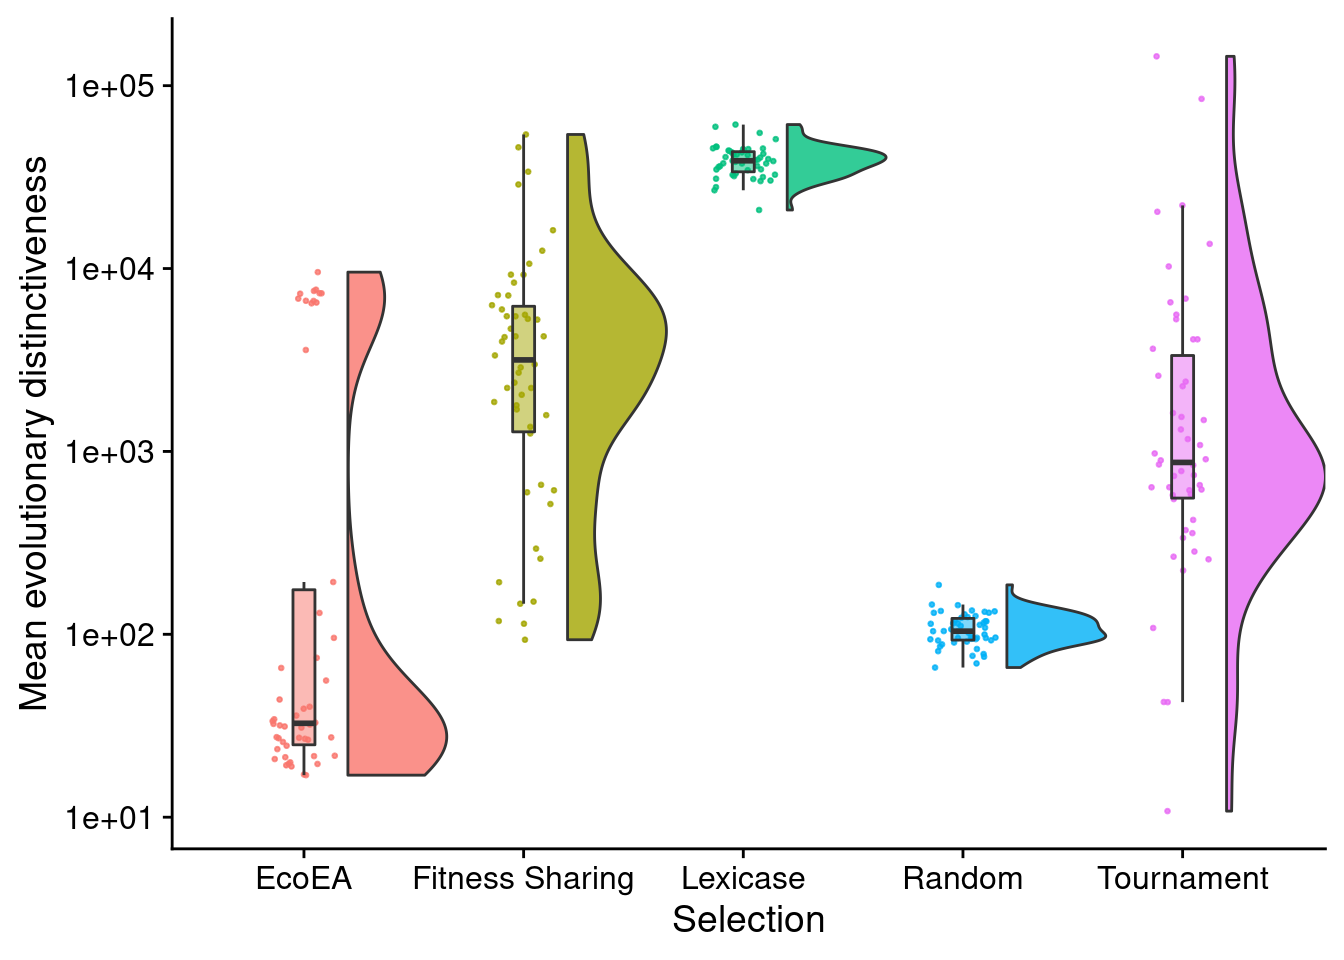
\includegraphics{phylodiversity-in-EC-supplement_files/figure-latex/final_phylogeny_plot_med-1.pdf}

Again, this looks fairly similar to MPD, except that fitness sharing and tournament are higher.

\hypertarget{phenotypic-diversity}{%
\section{Phenotypic diversity}\label{phenotypic-diversity}}

Now we analyze phenotypic (i.e.~population-level) diversity. Here, we're defining phenotypes to only include the sites that are actively contributing to fitness. So the phenotype of {[}1,4,2,6,5,4,3,6,7{]} would be {[}0,0,0,6,5,4,3,0,0{]}. Note that phylogenetic trees are also built using this conception of phenotypes.

\hypertarget{relationship-between-different-types-of-phenotypic-diversity}{%
\subsection{Relationship between different types of phenotypic diversity}\label{relationship-between-different-types-of-phenotypic-diversity}}

First, we should assess the extent to which different metrics of phenotypic diversity are capturing different information.

\begin{Shaded}
\begin{Highlighting}[]
\KeywordTok{ggplot}\NormalTok{(}
\NormalTok{    data }\OperatorTok\StringTok{ }\KeywordTok{filter}\NormalTok{(gen}\OperatorTok{==}\DecValTok{500000}\NormalTok{),}
    \KeywordTok{aes}\NormalTok{(}
        \DataTypeTok{y=}\NormalTok{phen_diversity,}
        \DataTypeTok{x=}\NormalTok{phen_num_taxa,}
        \DataTypeTok{color=}\NormalTok{selection_name,}
        \DataTypeTok{fill=}\NormalTok{selection_name}
\NormalTok{    )}
\NormalTok{  ) }\OperatorTok{+}
\StringTok{  }\KeywordTok{geom_point}\NormalTok{() }\OperatorTok{+}
\StringTok{    }\KeywordTok{scale_y_continuous}\NormalTok{(}
        \DataTypeTok{name=}\StringTok{"Phenotypic shannon diversity"}
\NormalTok{  ) }\OperatorTok{+}
\StringTok{  }\KeywordTok{scale_x_continuous}\NormalTok{(}
        \DataTypeTok{name=}\StringTok{"Phenotypic richness"}\NormalTok{,}
        \DataTypeTok{breaks =} \KeywordTok{breaks_extended}\NormalTok{(}\DecValTok{4}\NormalTok{)}
\NormalTok{  ) }\OperatorTok{+}\StringTok{ }
\StringTok{  }\KeywordTok{facet_wrap}\NormalTok{(}
      \OperatorTok{~}\NormalTok{selection_name, }\DataTypeTok{scales=}\StringTok{"free"}
\NormalTok{  ) }\OperatorTok{+}\StringTok{ }
\StringTok{  }\KeywordTok{stat_smooth}\NormalTok{(}
    \DataTypeTok{method=}\StringTok{"lm"}
\NormalTok{  ) }\OperatorTok{+}\StringTok{ }
\StringTok{  }\KeywordTok{stat_cor}\NormalTok{(}
    \DataTypeTok{method=}\StringTok{"spearman"}\NormalTok{, }\DataTypeTok{cor.coef.name =} \StringTok{"rho"}\NormalTok{, }\DataTypeTok{color=}\StringTok{"black"}
\NormalTok{  ) }\OperatorTok{+}
\StringTok{  }\KeywordTok{theme}\NormalTok{(}\DataTypeTok{legend.position =} \StringTok{"none"}\NormalTok{)}
\end{Highlighting}
\end{Shaded}

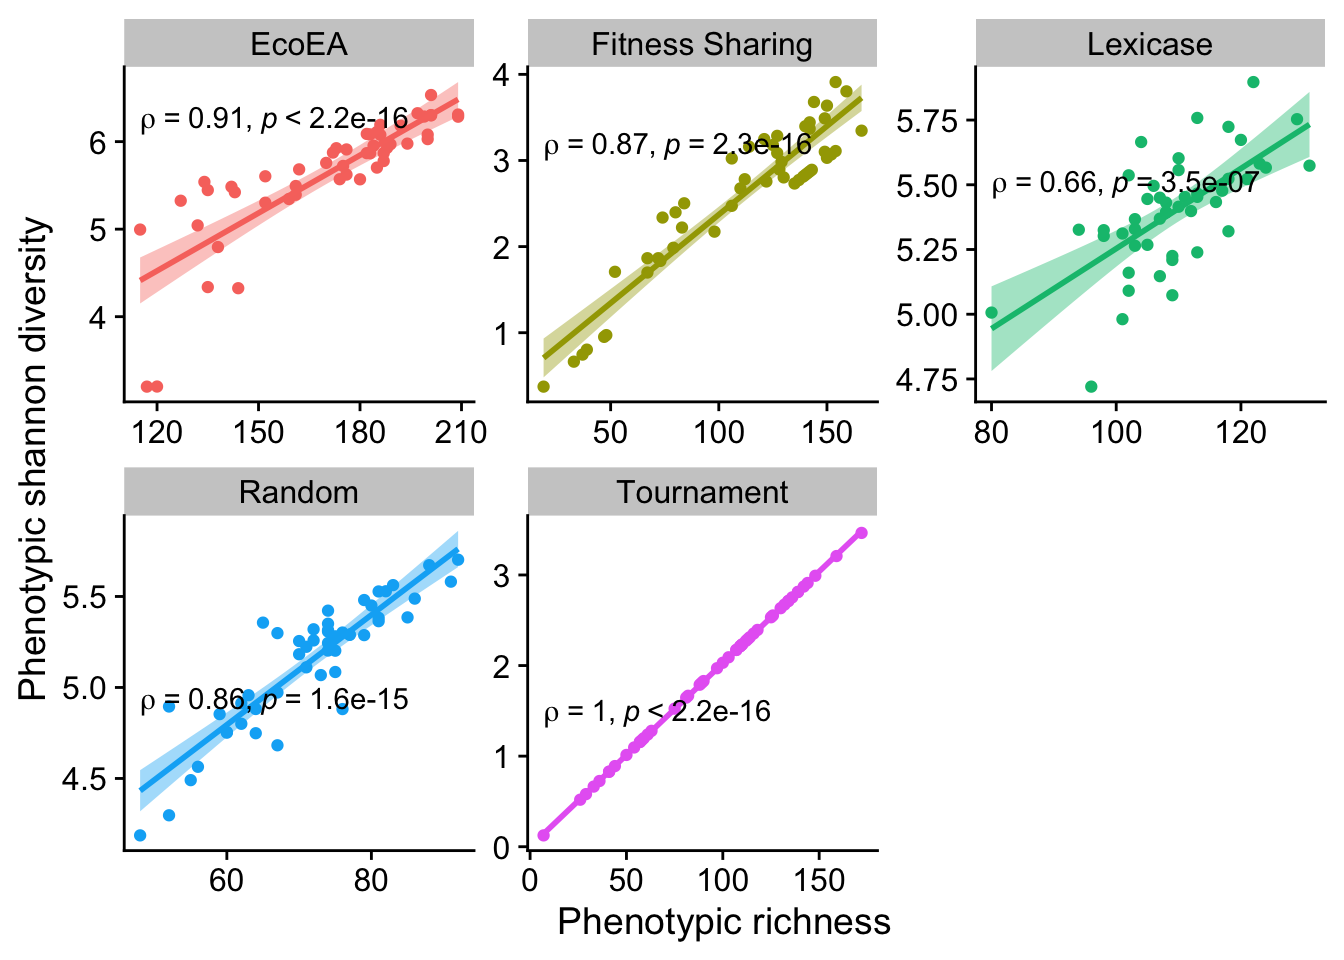
\includegraphics{phylodiversity-in-EC-supplement_files/figure-latex/richness_vs_shannon-1.pdf}

Looks like at the final time point they are pretty much always closely correlated, although this correlation is weaker for lexicase selection than for other selection schemes.

\hypertarget{over-time-2}{%
\subsection{Over time}\label{over-time-2}}

Now we examine the behavior of each phenotypic diversity metric over time.

\hypertarget{richness}{%
\subsubsection{Richness}\label{richness}}

\begin{Shaded}
\begin{Highlighting}[]
\KeywordTok{ggplot}\NormalTok{(}
\NormalTok{    data,}
    \KeywordTok{aes}\NormalTok{(}
      \DataTypeTok{x=}\NormalTok{gen,}
      \DataTypeTok{y=}\NormalTok{phen_num_taxa,}
      \DataTypeTok{color=}\NormalTok{selection_name,}
      \DataTypeTok{fill=}\NormalTok{selection_name}
\NormalTok{    )}
\NormalTok{  ) }\OperatorTok{+}
\StringTok{  }\KeywordTok{stat_summary}\NormalTok{(}\DataTypeTok{geom=}\StringTok{"line"}\NormalTok{, }\DataTypeTok{fun=}\NormalTok{mean) }\OperatorTok{+}
\StringTok{  }\KeywordTok{stat_summary}\NormalTok{(}
    \DataTypeTok{geom=}\StringTok{"ribbon"}\NormalTok{,}
    \DataTypeTok{fun.data=}\StringTok{"mean_cl_boot"}\NormalTok{,}
    \DataTypeTok{fun.args=}\KeywordTok{list}\NormalTok{(}\DataTypeTok{conf.int=}\FloatTok{0.95}\NormalTok{),}
    \DataTypeTok{alpha=}\FloatTok{0.2}\NormalTok{,}
    \DataTypeTok{linetype=}\DecValTok{0}
\NormalTok{  ) }\OperatorTok{+}
\StringTok{  }\KeywordTok{scale_y_continuous}\NormalTok{(}
    \DataTypeTok{name=}\StringTok{"Phenotypic richness"}
\NormalTok{  ) }\OperatorTok{+}
\StringTok{  }\KeywordTok{scale_x_log10}\NormalTok{(}
    \DataTypeTok{name=}\StringTok{"Generation"}
\NormalTok{  ) }\OperatorTok{+}
\StringTok{  }\KeywordTok{scale_color_discrete}\NormalTok{(}\StringTok{"Selection"}\NormalTok{) }\OperatorTok{+}\StringTok{ }
\StringTok{  }\KeywordTok{scale_fill_discrete}\NormalTok{(}\StringTok{"Selection"}\NormalTok{)}
\end{Highlighting}
\end{Shaded}

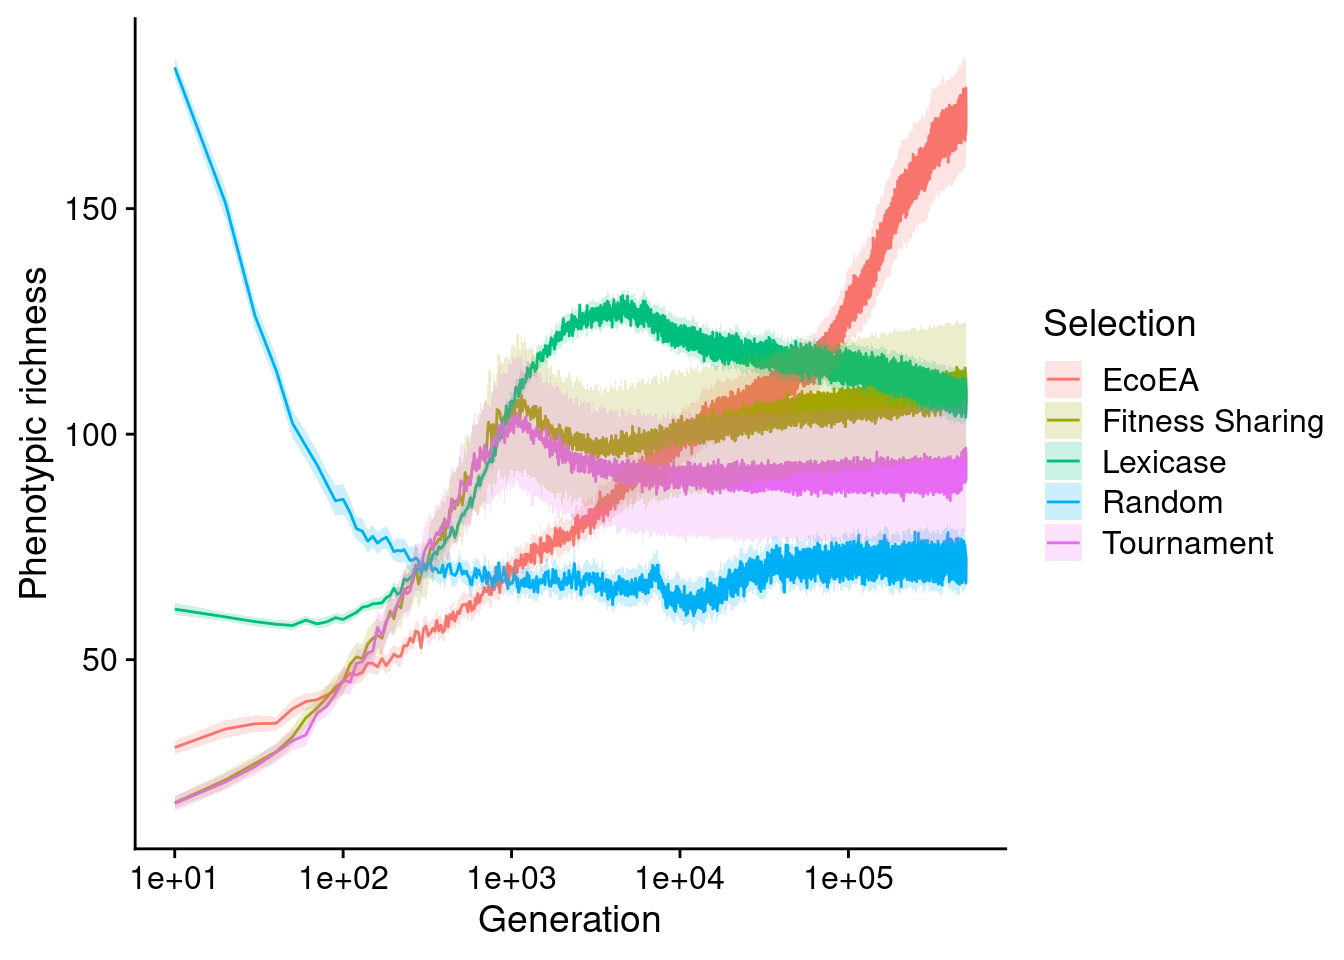
\includegraphics{phylodiversity-in-EC-supplement_files/figure-latex/phenotypic_diversity_over_time_plot-1.pdf}

In contrast to the phylodiversity results, phenotypic richness in all selection schemes (even tournament selection) ultimately exceeds that of random selection. Eco-EA monotonically increases while lexicase selection reaches a maximum around the same time it reaches its fitness plateau. The only real similarity to the phylodiversity results is the behavior tournament selection and fitness sharing relative to each other.

\hypertarget{shannon-diversity}{%
\subsubsection{Shannon diversity}\label{shannon-diversity}}

We also looked at phenotypic shannon diversity:

\begin{Shaded}
\begin{Highlighting}[]
\KeywordTok{ggplot}\NormalTok{(}
\NormalTok{    data,}
    \KeywordTok{aes}\NormalTok{(}
      \DataTypeTok{x=}\NormalTok{gen,}
      \DataTypeTok{y=}\NormalTok{phen_diversity,}
      \DataTypeTok{color=}\NormalTok{selection_name,}
      \DataTypeTok{fill=}\NormalTok{selection_name}
\NormalTok{    )}
\NormalTok{  ) }\OperatorTok{+}
\StringTok{  }\KeywordTok{stat_summary}\NormalTok{(}\DataTypeTok{geom=}\StringTok{"line"}\NormalTok{, }\DataTypeTok{fun=}\NormalTok{mean) }\OperatorTok{+}
\StringTok{  }\KeywordTok{stat_summary}\NormalTok{(}
    \DataTypeTok{geom=}\StringTok{"ribbon"}\NormalTok{,}
    \DataTypeTok{fun.data=}\StringTok{"mean_cl_boot"}\NormalTok{,}
    \DataTypeTok{fun.args=}\KeywordTok{list}\NormalTok{(}\DataTypeTok{conf.int=}\FloatTok{0.95}\NormalTok{),}
    \DataTypeTok{alpha=}\FloatTok{0.2}\NormalTok{,}
    \DataTypeTok{linetype=}\DecValTok{0}
\NormalTok{  ) }\OperatorTok{+}
\StringTok{  }\KeywordTok{scale_y_continuous}\NormalTok{(}
    \DataTypeTok{name=}\StringTok{"Phenotypic Shannon entropy"}
\NormalTok{  ) }\OperatorTok{+}
\StringTok{  }\KeywordTok{scale_x_log10}\NormalTok{(}
    \DataTypeTok{name=}\StringTok{"Generation"}
\NormalTok{  ) }\OperatorTok{+}
\StringTok{  }\KeywordTok{scale_color_discrete}\NormalTok{(}\StringTok{"Selection"}\NormalTok{) }\OperatorTok{+}\StringTok{ }
\StringTok{  }\KeywordTok{scale_fill_discrete}\NormalTok{(}\StringTok{"Selection"}\NormalTok{)}
\end{Highlighting}
\end{Shaded}

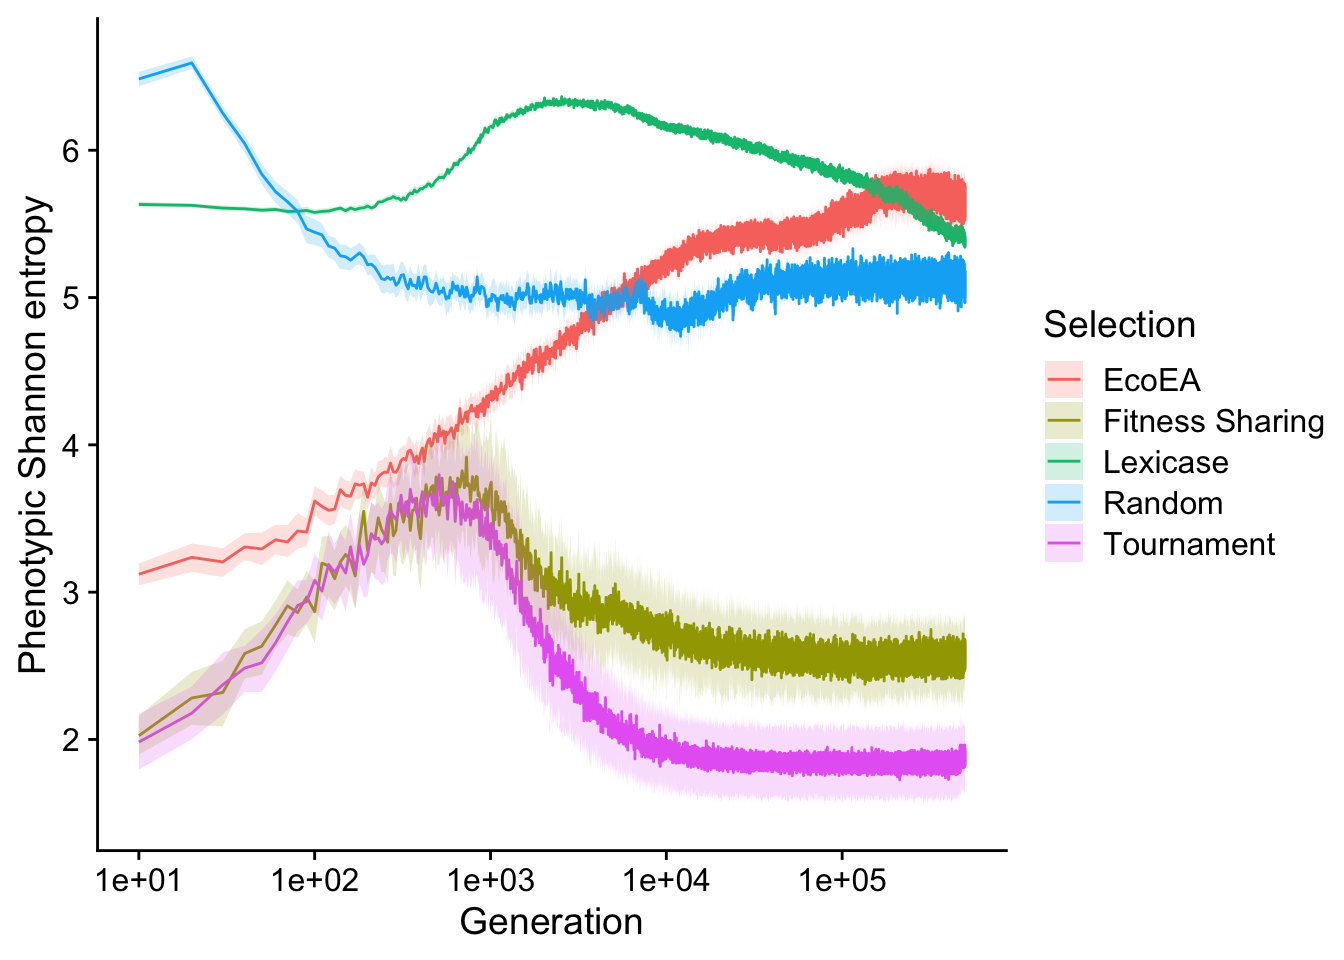
\includegraphics{phylodiversity-in-EC-supplement_files/figure-latex/phenotypic_diversity_over_time_plot_shannon-1.pdf}

This is more different from the richness results than we might have expected based on the correlation at the final time point. There is a much more pronounced drop off in Shannon entropy for tournament and fitness sharing than in richness. This difference is probably driven by the fact that, after plateauing, these selection schemes are likely both at mutation-selection balance. Thus, there are very many single-mutant phenotypes with only one copy in the population. These do not contribute much to Shannon entropy or phylogenetic diversity, but it does show up in richness.

We also see that, after plataeuing, lexicase selection does actually start to decrease in Shannon entropy, but slowly. Similarly, in Eco-EA, the increase in Shannon entropy towards the end is much more modest than the increase in richness.

\hypertarget{final-2}{%
\subsection{Final}\label{final-2}}

Now we assess the final phenotypic diversity

\hypertarget{richness-1}{%
\subsubsection{Richness}\label{richness-1}}

Hypothesis-testing differences between groups:

\begin{Shaded}
\begin{Highlighting}[]
\CommentTok{# Determine which conditions are significantly diferrent from each other}
\NormalTok{stat.test <-}\StringTok{ }\NormalTok{final_data }\OperatorTok
\StringTok{  }\KeywordTok{wilcox_test}\NormalTok{(phen_num_taxa }\OperatorTok{~}\StringTok{ }\NormalTok{selection_name) }\OperatorTok
\StringTok{  }\KeywordTok{adjust_pvalue}\NormalTok{(}\DataTypeTok{method =} \StringTok{"bonferroni"}\NormalTok{) }\OperatorTok
\StringTok{  }\KeywordTok{add_significance}\NormalTok{() }\OperatorTok
\StringTok{  }\KeywordTok{add_xy_position}\NormalTok{(}\DataTypeTok{x=}\StringTok{"selection_name"}\NormalTok{,}\DataTypeTok{step.increase=}\DecValTok{1}\NormalTok{)}
\NormalTok{stat.test}\OperatorTok{$}\NormalTok{label <-}\StringTok{ }\KeywordTok{mapply}\NormalTok{(p_label,stat.test}\OperatorTok{$}\NormalTok{p.adj)}

\NormalTok{stat.test }\OperatorTok
\StringTok{  }\KeywordTok{kbl}\NormalTok{() }\OperatorTok
\StringTok{  }\KeywordTok{kable_styling}\NormalTok{(}
    \DataTypeTok{bootstrap_options =} \KeywordTok{c}\NormalTok{(}
      \StringTok{"striped"}\NormalTok{,}
      \StringTok{"hover"}\NormalTok{,}
      \StringTok{"condensed"}\NormalTok{,}
      \StringTok{"responsive"}
\NormalTok{    )}
\NormalTok{  ) }\OperatorTok
\StringTok{  }\KeywordTok{scroll_box}\NormalTok{(}\DataTypeTok{width=}\StringTok{"600px"}\NormalTok{)}
\end{Highlighting}
\end{Shaded}

\begin{table}
\centering
\begin{tabular}[t]{l|l|l|r|r|r|r|r|l|r|l|r|r|l}
\hline
.y. & group1 & group2 & n1 & n2 & statistic & p & p.adj & p.adj.signif & y.position & groups & xmin & xmax & label\\
\hline
phen\_num\_taxa & EcoEA & Fitness Sharing & 50 & 50 & 2249.0 & 0.00e+00 & 0.0e+00 & **** & 326 & EcoEA          , Fitness Sharing & 1 & 2 & p < 1e-04\\
\hline
phen\_num\_taxa & EcoEA & Lexicase & 50 & 47 & 2319.0 & 0.00e+00 & 0.0e+00 & **** & 456 & EcoEA   , Lexicase & 1 & 3 & p < 1e-04\\
\hline
phen\_num\_taxa & EcoEA & Random & 50 & 50 & 2500.0 & 0.00e+00 & 0.0e+00 & **** & 586 & EcoEA , Random & 1 & 4 & p < 1e-04\\
\hline
phen\_num\_taxa & EcoEA & Tournament & 50 & 50 & 2378.5 & 0.00e+00 & 0.0e+00 & **** & 716 & EcoEA     , Tournament & 1 & 5 & p < 1e-04\\
\hline
phen\_num\_taxa & Fitness Sharing & Lexicase & 50 & 47 & 1428.0 & 6.80e-02 & 6.8e-01 & ns & 846 & Fitness Sharing, Lexicase & 2 & 3 & p = 0.68\\
\hline
phen\_num\_taxa & Fitness Sharing & Random & 50 & 50 & 1973.0 & 6.00e-07 & 6.3e-06 & **** & 976 & Fitness Sharing, Random & 2 & 4 & p < 1e-04\\
\hline
phen\_num\_taxa & Fitness Sharing & Tournament & 50 & 50 & 1585.0 & 2.10e-02 & 2.1e-01 & ns & 1106 & Fitness Sharing, Tournament & 2 & 5 & p = 0.21\\
\hline
phen\_num\_taxa & Lexicase & Random & 47 & 50 & 2339.5 & 0.00e+00 & 0.0e+00 & **** & 1236 & Lexicase, Random & 3 & 4 & p < 1e-04\\
\hline
phen\_num\_taxa & Lexicase & Tournament & 47 & 50 & 1359.0 & 1.85e-01 & 1.0e+00 & ns & 1366 & Lexicase  , Tournament & 3 & 5 & p = 1\\
\hline
phen\_num\_taxa & Random & Tournament & 50 & 50 & 797.0 & 2.00e-03 & 2.0e-02 & * & 1496 & Random    , Tournament & 4 & 5 & p = 0.02\\
\hline
\end{tabular}
\end{table}

Raincloud plot:

\begin{Shaded}
\begin{Highlighting}[]
\CommentTok{# Raincloud plot of final phenotypic diversity}
\NormalTok{final_phenotypic_fig <-}\StringTok{ }\KeywordTok{ggplot}\NormalTok{(}
\NormalTok{    final_data,}
    \KeywordTok{aes}\NormalTok{(}
      \DataTypeTok{x=}\NormalTok{selection_name,}
      \DataTypeTok{y=}\NormalTok{phen_num_taxa,}
      \DataTypeTok{fill=}\NormalTok{selection_name}
\NormalTok{    )}
\NormalTok{  ) }\OperatorTok{+}
\StringTok{  }\KeywordTok{geom_flat_violin}\NormalTok{(}
    \DataTypeTok{position =} \KeywordTok{position_nudge}\NormalTok{(}\DataTypeTok{x =} \FloatTok{.2}\NormalTok{, }\DataTypeTok{y =} \DecValTok{0}\NormalTok{),}
    \DataTypeTok{alpha =} \FloatTok{.8}\NormalTok{,}
    \DataTypeTok{scale=}\StringTok{"width"}
\NormalTok{  ) }\OperatorTok{+}
\StringTok{  }\KeywordTok{geom_point}\NormalTok{(}
    \DataTypeTok{mapping=}\KeywordTok{aes}\NormalTok{(}\DataTypeTok{color=}\NormalTok{selection_name),}
    \DataTypeTok{position =} \KeywordTok{position_jitter}\NormalTok{(}\DataTypeTok{width =} \FloatTok{.15}\NormalTok{),}
    \DataTypeTok{size =} \FloatTok{.5}\NormalTok{,}
    \DataTypeTok{alpha =} \FloatTok{0.8}
\NormalTok{  ) }\OperatorTok{+}
\StringTok{  }\KeywordTok{geom_boxplot}\NormalTok{(}
    \DataTypeTok{width =} \FloatTok{.1}\NormalTok{,}
    \DataTypeTok{outlier.shape =} \OtherTok{NA}\NormalTok{,}
    \DataTypeTok{alpha =} \FloatTok{0.5}
\NormalTok{  ) }\OperatorTok{+}
\StringTok{  }\KeywordTok{scale_y_continuous}\NormalTok{(}
    \DataTypeTok{name=}\StringTok{"Phenotypic Richness"}
\NormalTok{  ) }\OperatorTok{+}
\StringTok{  }\KeywordTok{scale_x_discrete}\NormalTok{(}
    \DataTypeTok{name=}\StringTok{"Selection"}
\NormalTok{  ) }\OperatorTok{+}
\StringTok{  }\KeywordTok{scale_fill_discrete}\NormalTok{(}
    \DataTypeTok{name=}\StringTok{"Selection"}
\NormalTok{  ) }\OperatorTok{+}
\StringTok{  }\KeywordTok{scale_color_discrete}\NormalTok{(}
    \DataTypeTok{name=}\StringTok{"Selection"}
\NormalTok{  ) }\OperatorTok{+}
\StringTok{  }\KeywordTok{theme}\NormalTok{(}\DataTypeTok{legend.position =} \StringTok{"none"}\NormalTok{)}
\NormalTok{final_phenotypic_fig}
\end{Highlighting}
\end{Shaded}

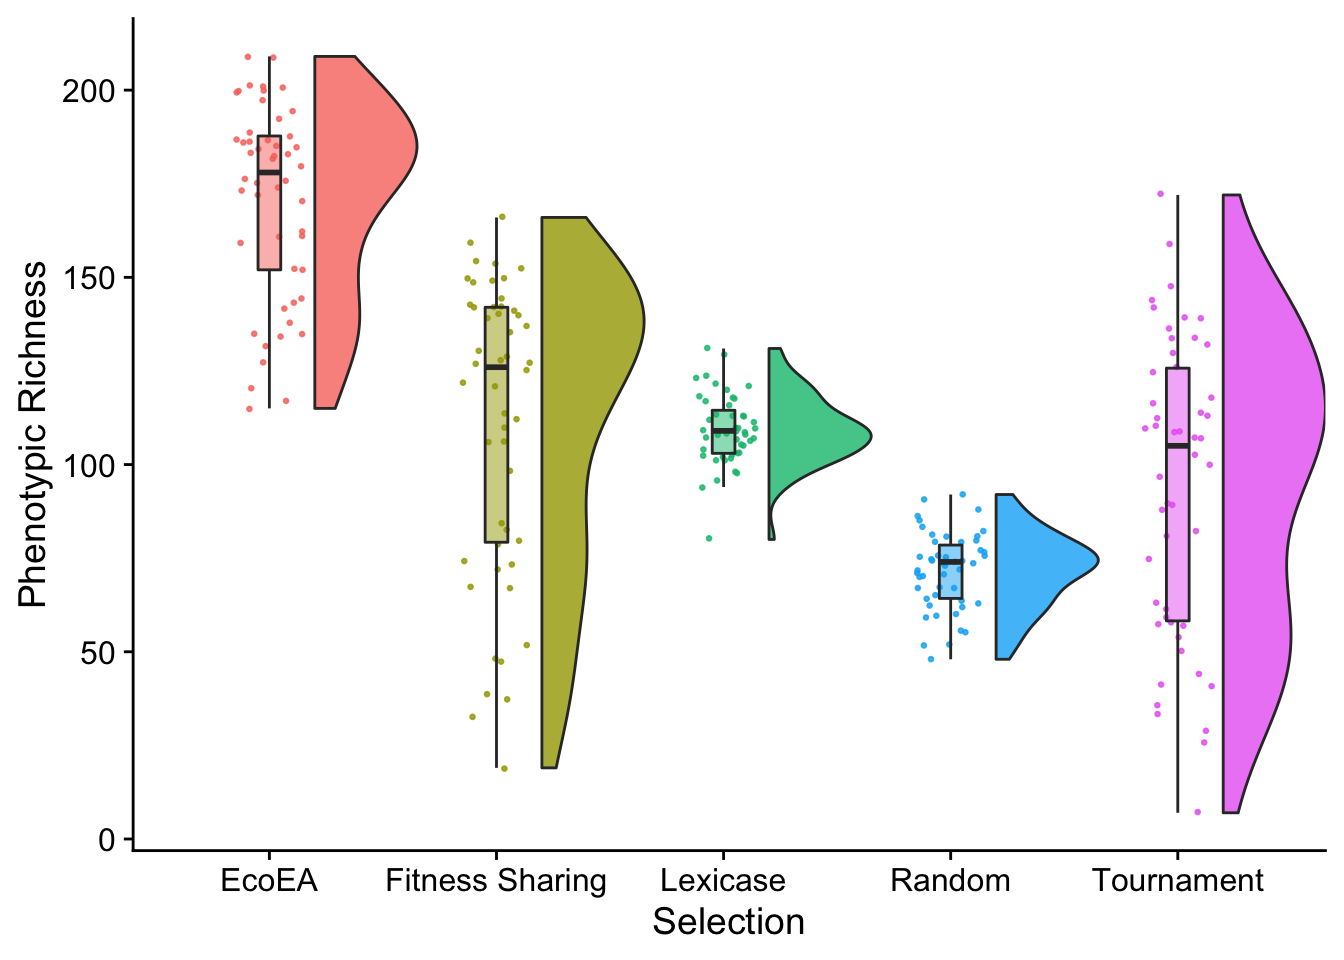
\includegraphics{phylodiversity-in-EC-supplement_files/figure-latex/final_phenotypic_plot-1.pdf}

Nothing particularly suprising here, but we should note that, based on the over time plot, this would look a lot different if we had selected a different time point.

\hypertarget{shannon-diversity-1}{%
\subsubsection{Shannon diversity}\label{shannon-diversity-1}}

\begin{Shaded}
\begin{Highlighting}[]
\CommentTok{# Determine which conditions are significantly diferrent from each other}
\NormalTok{stat.test <-}\StringTok{ }\NormalTok{final_data }\OperatorTok
\StringTok{  }\KeywordTok{wilcox_test}\NormalTok{(phen_diversity}\OperatorTok{~}\StringTok{ }\NormalTok{selection_name) }\OperatorTok
\StringTok{  }\KeywordTok{adjust_pvalue}\NormalTok{(}\DataTypeTok{method =} \StringTok{"bonferroni"}\NormalTok{) }\OperatorTok
\StringTok{  }\KeywordTok{add_significance}\NormalTok{() }\OperatorTok
\StringTok{  }\KeywordTok{add_xy_position}\NormalTok{(}\DataTypeTok{x=}\StringTok{"selection_name"}\NormalTok{,}\DataTypeTok{step.increase=}\DecValTok{1}\NormalTok{)}
\NormalTok{stat.test}\OperatorTok{$}\NormalTok{label <-}\StringTok{ }\KeywordTok{mapply}\NormalTok{(p_label,stat.test}\OperatorTok{$}\NormalTok{p.adj)}

\NormalTok{stat.test }\OperatorTok
\StringTok{  }\KeywordTok{kbl}\NormalTok{() }\OperatorTok
\StringTok{  }\KeywordTok{kable_styling}\NormalTok{(}
    \DataTypeTok{bootstrap_options =} \KeywordTok{c}\NormalTok{(}
      \StringTok{"striped"}\NormalTok{,}
      \StringTok{"hover"}\NormalTok{,}
      \StringTok{"condensed"}\NormalTok{,}
      \StringTok{"responsive"}
\NormalTok{    )}
\NormalTok{  ) }\OperatorTok
\StringTok{  }\KeywordTok{scroll_box}\NormalTok{(}\DataTypeTok{width=}\StringTok{"600px"}\NormalTok{)}
\end{Highlighting}
\end{Shaded}

\begin{table}
\centering
\begin{tabular}[t]{l|l|l|r|r|r|r|r|l|r|l|r|r|l}
\hline
.y. & group1 & group2 & n1 & n2 & statistic & p & p.adj & p.adj.signif & y.position & groups & xmin & xmax & label\\
\hline
phen\_diversity & EcoEA & Fitness Sharing & 50 & 50 & 2478.0 & 0.00e+00 & 0.00e+00 & **** & 9.602 & EcoEA          , Fitness Sharing & 1 & 2 & p < 1e-04\\
\hline
phen\_diversity & EcoEA & Lexicase & 50 & 47 & 1772.0 & 1.66e-05 & 1.66e-04 & *** & 13.012 & EcoEA   , Lexicase & 1 & 3 & p = 0.000166\\
\hline
phen\_diversity & EcoEA & Random & 50 & 50 & 2089.5 & 0.00e+00 & 1.00e-07 & **** & 16.422 & EcoEA , Random & 1 & 4 & p < 1e-04\\
\hline
phen\_diversity & EcoEA & Tournament & 50 & 50 & 2496.0 & 0.00e+00 & 0.00e+00 & **** & 19.832 & EcoEA     , Tournament & 1 & 5 & p < 1e-04\\
\hline
phen\_diversity & Fitness Sharing & Lexicase & 50 & 47 & 0.0 & 0.00e+00 & 0.00e+00 & **** & 23.242 & Fitness Sharing, Lexicase & 2 & 3 & p < 1e-04\\
\hline
phen\_diversity & Fitness Sharing & Random & 50 & 50 & 0.0 & 0.00e+00 & 0.00e+00 & **** & 26.652 & Fitness Sharing, Random & 2 & 4 & p < 1e-04\\
\hline
phen\_diversity & Fitness Sharing & Tournament & 50 & 50 & 1856.0 & 2.99e-05 & 2.99e-04 & *** & 30.062 & Fitness Sharing, Tournament & 2 & 5 & p = 0.000299\\
\hline
phen\_diversity & Lexicase & Random & 47 & 50 & 1714.0 & 1.01e-04 & 1.01e-03 & ** & 33.472 & Lexicase, Random & 3 & 4 & p = 0.00101\\
\hline
phen\_diversity & Lexicase & Tournament & 47 & 50 & 2350.0 & 0.00e+00 & 0.00e+00 & **** & 36.882 & Lexicase  , Tournament & 3 & 5 & p < 1e-04\\
\hline
phen\_diversity & Random & Tournament & 50 & 50 & 2500.0 & 0.00e+00 & 0.00e+00 & **** & 40.292 & Random    , Tournament & 4 & 5 & p < 1e-04\\
\hline
\end{tabular}
\end{table}

Interestingly, the final shannon diversity values of different selection schemes are much more distinguishable from each other than the final richness values.

\begin{Shaded}
\begin{Highlighting}[]
\CommentTok{# Raincloud plot of final phenotypic diversity}
\KeywordTok{ggplot}\NormalTok{(}
\NormalTok{    final_data,}
    \KeywordTok{aes}\NormalTok{(}
      \DataTypeTok{x=}\NormalTok{selection_name,}
      \DataTypeTok{y=}\NormalTok{phen_num_taxa,}
      \DataTypeTok{fill=}\NormalTok{selection_name}
\NormalTok{    )}
\NormalTok{  ) }\OperatorTok{+}
\StringTok{  }\KeywordTok{geom_flat_violin}\NormalTok{(}
    \DataTypeTok{position =} \KeywordTok{position_nudge}\NormalTok{(}\DataTypeTok{x =} \FloatTok{.2}\NormalTok{, }\DataTypeTok{y =} \DecValTok{0}\NormalTok{),}
    \DataTypeTok{alpha =} \FloatTok{.8}\NormalTok{,}
    \DataTypeTok{scale=}\StringTok{"width"}
\NormalTok{  ) }\OperatorTok{+}
\StringTok{  }\KeywordTok{geom_point}\NormalTok{(}
    \DataTypeTok{mapping=}\KeywordTok{aes}\NormalTok{(}\DataTypeTok{color=}\NormalTok{selection_name),}
    \DataTypeTok{position =} \KeywordTok{position_jitter}\NormalTok{(}\DataTypeTok{width =} \FloatTok{.15}\NormalTok{),}
    \DataTypeTok{size =} \FloatTok{.5}\NormalTok{,}
    \DataTypeTok{alpha =} \FloatTok{0.8}
\NormalTok{  ) }\OperatorTok{+}
\StringTok{  }\KeywordTok{geom_boxplot}\NormalTok{(}
    \DataTypeTok{width =} \FloatTok{.1}\NormalTok{,}
    \DataTypeTok{outlier.shape =} \OtherTok{NA}\NormalTok{,}
    \DataTypeTok{alpha =} \FloatTok{0.5}
\NormalTok{  ) }\OperatorTok{+}
\StringTok{  }\KeywordTok{scale_y_continuous}\NormalTok{(}
    \DataTypeTok{name=}\StringTok{"Phenotypic Shannon Diversity"}
\NormalTok{  ) }\OperatorTok{+}
\StringTok{  }\KeywordTok{scale_x_discrete}\NormalTok{(}
    \DataTypeTok{name=}\StringTok{"Selection"}
\NormalTok{  ) }\OperatorTok{+}
\StringTok{  }\KeywordTok{scale_fill_discrete}\NormalTok{(}
    \DataTypeTok{name=}\StringTok{"Selection"}
\NormalTok{  ) }\OperatorTok{+}
\StringTok{  }\KeywordTok{scale_color_discrete}\NormalTok{(}
    \DataTypeTok{name=}\StringTok{"Selection"}
\NormalTok{  ) }\OperatorTok{+}
\StringTok{  }\KeywordTok{theme}\NormalTok{(}\DataTypeTok{legend.position =} \StringTok{"none"}\NormalTok{)}
\end{Highlighting}
\end{Shaded}

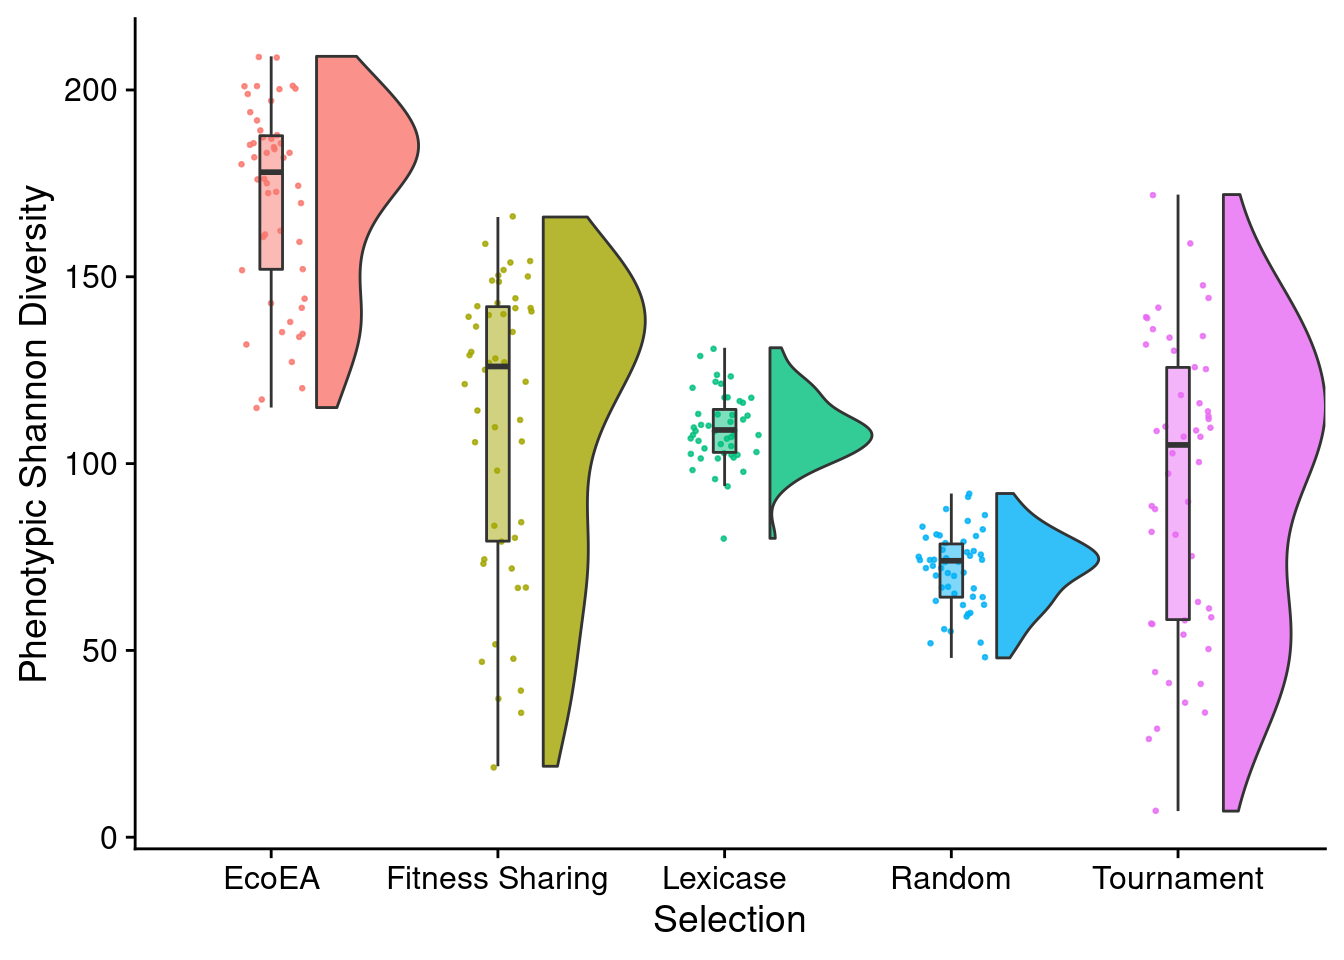
\includegraphics{phylodiversity-in-EC-supplement_files/figure-latex/final_phenotypic_plot_shannon-1.pdf}

Again, we know from the time series plots that these relative relationships varied a lot over time. Eco-EA is only higher than lexicase selection at the very end.

\hypertarget{relationship-between-phenotypic-and-phylogenetic-diversity}{%
\section{Relationship between phenotypic and phylogenetic diversity}\label{relationship-between-phenotypic-and-phylogenetic-diversity}}

Now, we can finally begin to address the main questions. Do phenotypic diversity and phylogenetic diversity capture different information?

\hypertarget{phenotypic-richness-vs.mean-pairwise-distance}{%
\subsection{Phenotypic richness vs.~mean pairwise distance}\label{phenotypic-richness-vs.mean-pairwise-distance}}

\begin{Shaded}
\begin{Highlighting}[]
\KeywordTok{ggplot}\NormalTok{(}
\NormalTok{    data }\OperatorTok\StringTok{ }\KeywordTok{filter}\NormalTok{(gen}\OperatorTok{==}\DecValTok{500000}\NormalTok{),}
    \KeywordTok{aes}\NormalTok{(}
        \DataTypeTok{y=}\NormalTok{phen_num_taxa,}
        \DataTypeTok{x=}\NormalTok{mean_phenotype_pairwise_distance,}
        \DataTypeTok{color=}\NormalTok{selection_name,}
        \DataTypeTok{fill=}\NormalTok{selection_name}
\NormalTok{    )}
\NormalTok{  ) }\OperatorTok{+}
\StringTok{  }\KeywordTok{geom_point}\NormalTok{() }\OperatorTok{+}
\StringTok{    }\KeywordTok{scale_y_continuous}\NormalTok{(}
        \DataTypeTok{name=}\StringTok{"Phenotypic richness"}
\NormalTok{  ) }\OperatorTok{+}
\StringTok{  }\KeywordTok{scale_x_continuous}\NormalTok{(}
        \DataTypeTok{name=}\StringTok{"Mean pairwise distance"}\NormalTok{,}
        \DataTypeTok{breaks =} \KeywordTok{breaks_extended}\NormalTok{(}\DecValTok{4}\NormalTok{)}
\NormalTok{  ) }\OperatorTok{+}\StringTok{ }
\StringTok{  }\KeywordTok{facet_wrap}\NormalTok{(}
      \OperatorTok{~}\NormalTok{selection_name, }\DataTypeTok{scales=}\StringTok{"free"}
\NormalTok{  ) }\OperatorTok{+}\StringTok{ }
\StringTok{  }\KeywordTok{stat_smooth}\NormalTok{(}
    \DataTypeTok{method=}\StringTok{"lm"}
\NormalTok{  ) }\OperatorTok{+}\StringTok{ }
\StringTok{  }\KeywordTok{stat_cor}\NormalTok{(}
    \DataTypeTok{method=}\StringTok{"spearman"}\NormalTok{, }\DataTypeTok{cor.coef.name =} \StringTok{"rho"}\NormalTok{, }\DataTypeTok{color=}\StringTok{"black"}
\NormalTok{  ) }\OperatorTok{+}
\StringTok{  }\KeywordTok{theme}\NormalTok{(}\DataTypeTok{legend.position =} \StringTok{"none"}\NormalTok{)}
\end{Highlighting}
\end{Shaded}

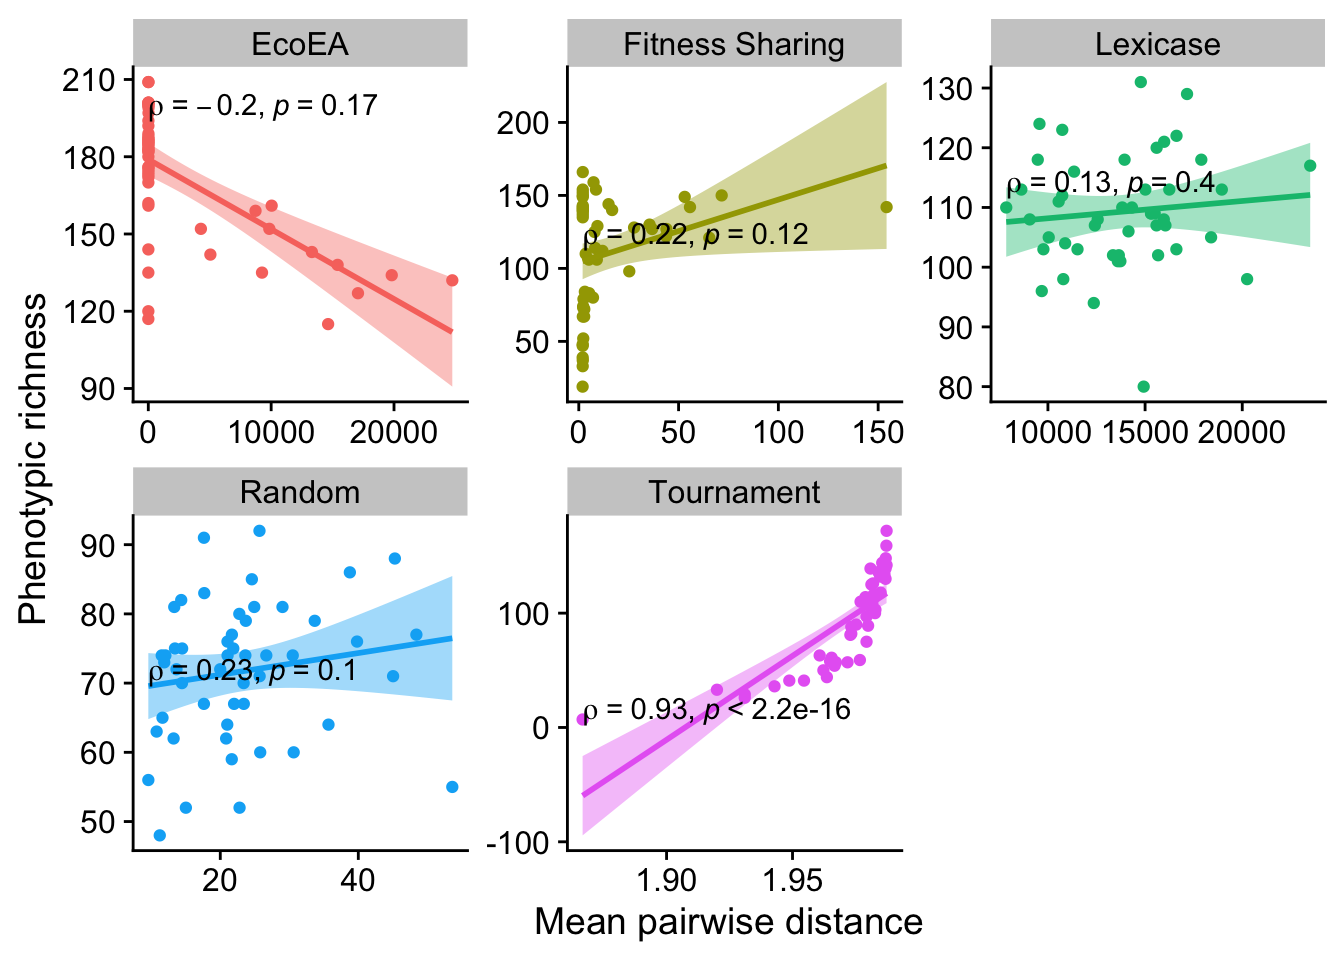
\includegraphics{phylodiversity-in-EC-supplement_files/figure-latex/phen_vs_phylo_richness_mpd-1.pdf}

The linear models for some of these are questionable, but the Spearman correlation coefficient should be fine because it does not require linearity. Only tournament selection is significantly different from 0. Eco-EA is even negative (although non-significant), which is probably driven by the fact that there are really two groups of runs in Eco-EA: those that have found a good solution and had their diversity crash, and those that haven't yet.

Lets take a look at how each of those groups behave (we'll show fitness as color, just to better understand what's happening):

\begin{Shaded}
\begin{Highlighting}[]
\KeywordTok{ggplot}\NormalTok{(}
\NormalTok{    data }\OperatorTok\StringTok{ }\KeywordTok{filter}\NormalTok{(gen}\OperatorTok{==}\DecValTok{500000}\NormalTok{, selection_name }\OperatorTok{==}\StringTok{ "EcoEA"}\NormalTok{),}
    \KeywordTok{aes}\NormalTok{(}
        \DataTypeTok{y=}\NormalTok{phen_num_taxa,}
        \DataTypeTok{x=}\NormalTok{mean_phenotype_pairwise_distance,}
        \DataTypeTok{color =}\NormalTok{ elite_trait_avg}
\NormalTok{    )}
\NormalTok{  ) }\OperatorTok{+}
\StringTok{  }\KeywordTok{geom_point}\NormalTok{() }\OperatorTok{+}
\StringTok{    }\KeywordTok{scale_y_continuous}\NormalTok{(}
        \DataTypeTok{name=}\StringTok{"Phenotypic richness"}
\NormalTok{  ) }\OperatorTok{+}
\StringTok{  }\KeywordTok{scale_x_continuous}\NormalTok{(}
        \DataTypeTok{name=}\StringTok{"Mean pairwise distance"}\NormalTok{,}
        \DataTypeTok{breaks =} \KeywordTok{breaks_extended}\NormalTok{(}\DecValTok{4}\NormalTok{)}
\NormalTok{  ) }\OperatorTok{+}\StringTok{ }
\StringTok{  }\KeywordTok{facet_wrap}\NormalTok{(}
      \OperatorTok{~}\NormalTok{mean_phenotype_pairwise_distance }\OperatorTok{>}\StringTok{ }\DecValTok{100}\NormalTok{, }\DataTypeTok{scales=}\StringTok{"free"}
\NormalTok{  ) }\OperatorTok{+}\StringTok{ }
\StringTok{  }\KeywordTok{stat_smooth}\NormalTok{(}
    \DataTypeTok{method=}\StringTok{"lm"}
\NormalTok{  ) }\OperatorTok{+}\StringTok{ }
\StringTok{  }\KeywordTok{stat_cor}\NormalTok{(}
    \DataTypeTok{method=}\StringTok{"spearman"}\NormalTok{, }\DataTypeTok{cor.coef.name =} \StringTok{"rho"}\NormalTok{, }\DataTypeTok{color=}\StringTok{"black"}
\NormalTok{  ) }\OperatorTok{+}
\StringTok{  }\KeywordTok{scale_color_continuous}\NormalTok{(}\DataTypeTok{type=}\StringTok{"viridis"}\NormalTok{)}
\end{Highlighting}
\end{Shaded}

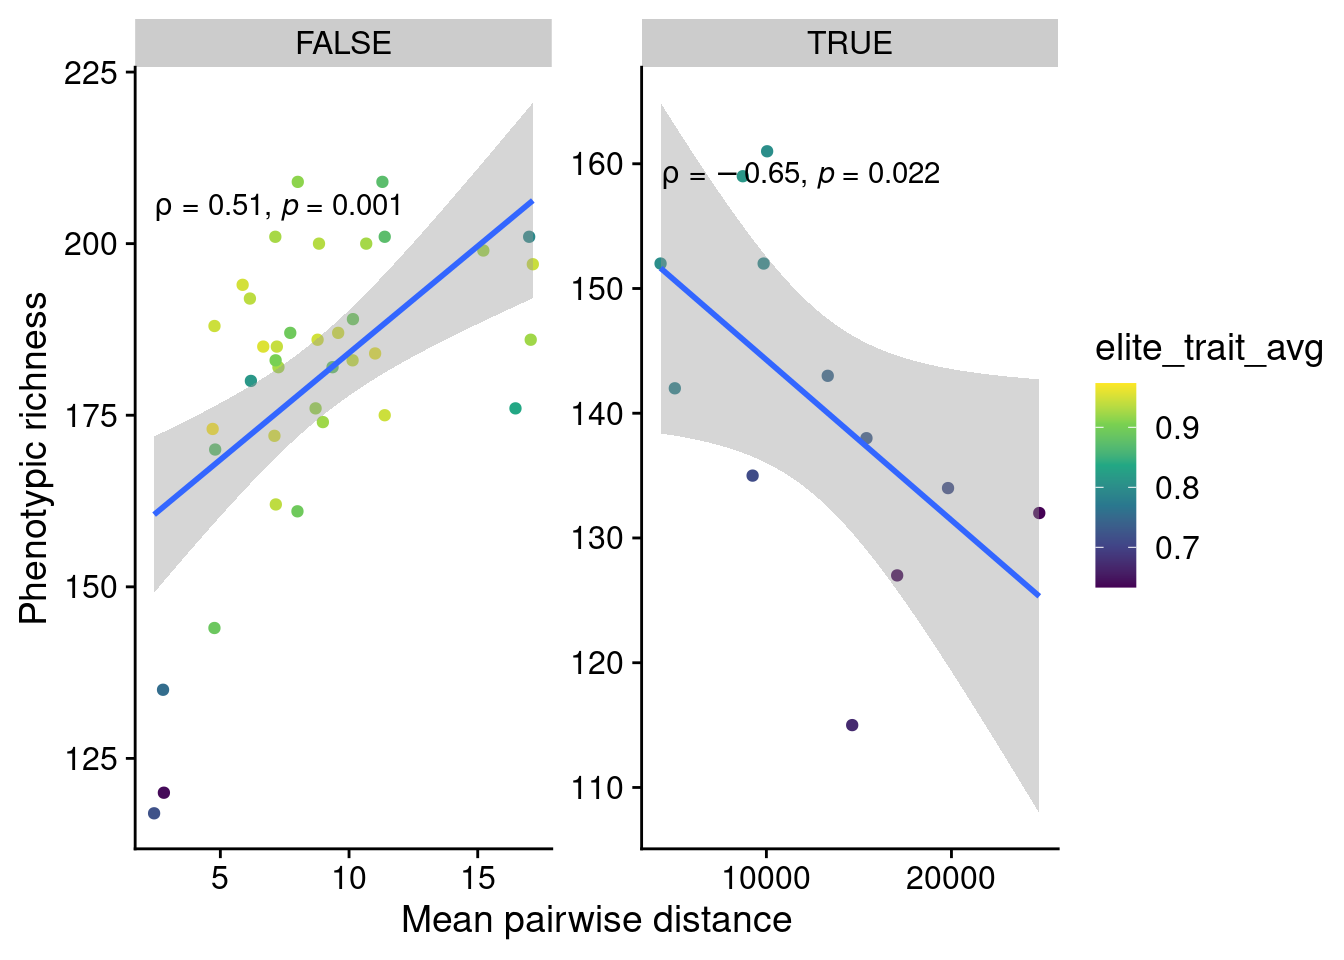
\includegraphics{phylodiversity-in-EC-supplement_files/figure-latex/eco_ea_zoom_in-1.pdf}

\hypertarget{phenotypic-richness-vs.mean-evolutionary-distinctiveness}{%
\subsection{Phenotypic richness vs.~mean evolutionary distinctiveness}\label{phenotypic-richness-vs.mean-evolutionary-distinctiveness}}

\begin{Shaded}
\begin{Highlighting}[]
\KeywordTok{ggplot}\NormalTok{(}
\NormalTok{    data }\OperatorTok\StringTok{ }\KeywordTok{filter}\NormalTok{(gen}\OperatorTok{==}\DecValTok{500000}\NormalTok{),}
    \KeywordTok{aes}\NormalTok{(}
        \DataTypeTok{y=}\NormalTok{phen_num_taxa,}
        \DataTypeTok{x=}\NormalTok{mean_phenotype_evolutionary_distinctiveness,}
        \DataTypeTok{color=}\NormalTok{selection_name,}
        \DataTypeTok{fill=}\NormalTok{selection_name}
\NormalTok{    )}
\NormalTok{  ) }\OperatorTok{+}
\StringTok{  }\KeywordTok{geom_point}\NormalTok{() }\OperatorTok{+}
\StringTok{    }\KeywordTok{scale_y_continuous}\NormalTok{(}
        \DataTypeTok{name=}\StringTok{"Phenotypic richness"}
\NormalTok{  ) }\OperatorTok{+}
\StringTok{  }\KeywordTok{scale_x_continuous}\NormalTok{(}
        \DataTypeTok{name=}\StringTok{"Mean evolutionary distinctiveness"}\NormalTok{,}
        \DataTypeTok{breaks =} \KeywordTok{breaks_extended}\NormalTok{(}\DecValTok{4}\NormalTok{)}
\NormalTok{  ) }\OperatorTok{+}\StringTok{ }
\StringTok{  }\KeywordTok{facet_wrap}\NormalTok{(}
      \OperatorTok{~}\NormalTok{selection_name, }\DataTypeTok{scales=}\StringTok{"free"}
\NormalTok{  ) }\OperatorTok{+}\StringTok{ }
\StringTok{  }\KeywordTok{stat_smooth}\NormalTok{(}
    \DataTypeTok{method=}\StringTok{"lm"}
\NormalTok{  ) }\OperatorTok{+}\StringTok{ }
\StringTok{  }\KeywordTok{stat_cor}\NormalTok{(}
    \DataTypeTok{method=}\StringTok{"spearman"}\NormalTok{, }\DataTypeTok{cor.coef.name =} \StringTok{"rho"}\NormalTok{, }\DataTypeTok{color=}\StringTok{"black"}
\NormalTok{  ) }\OperatorTok{+}
\StringTok{  }\KeywordTok{theme}\NormalTok{(}\DataTypeTok{legend.position =} \StringTok{"none"}\NormalTok{)}
\end{Highlighting}
\end{Shaded}

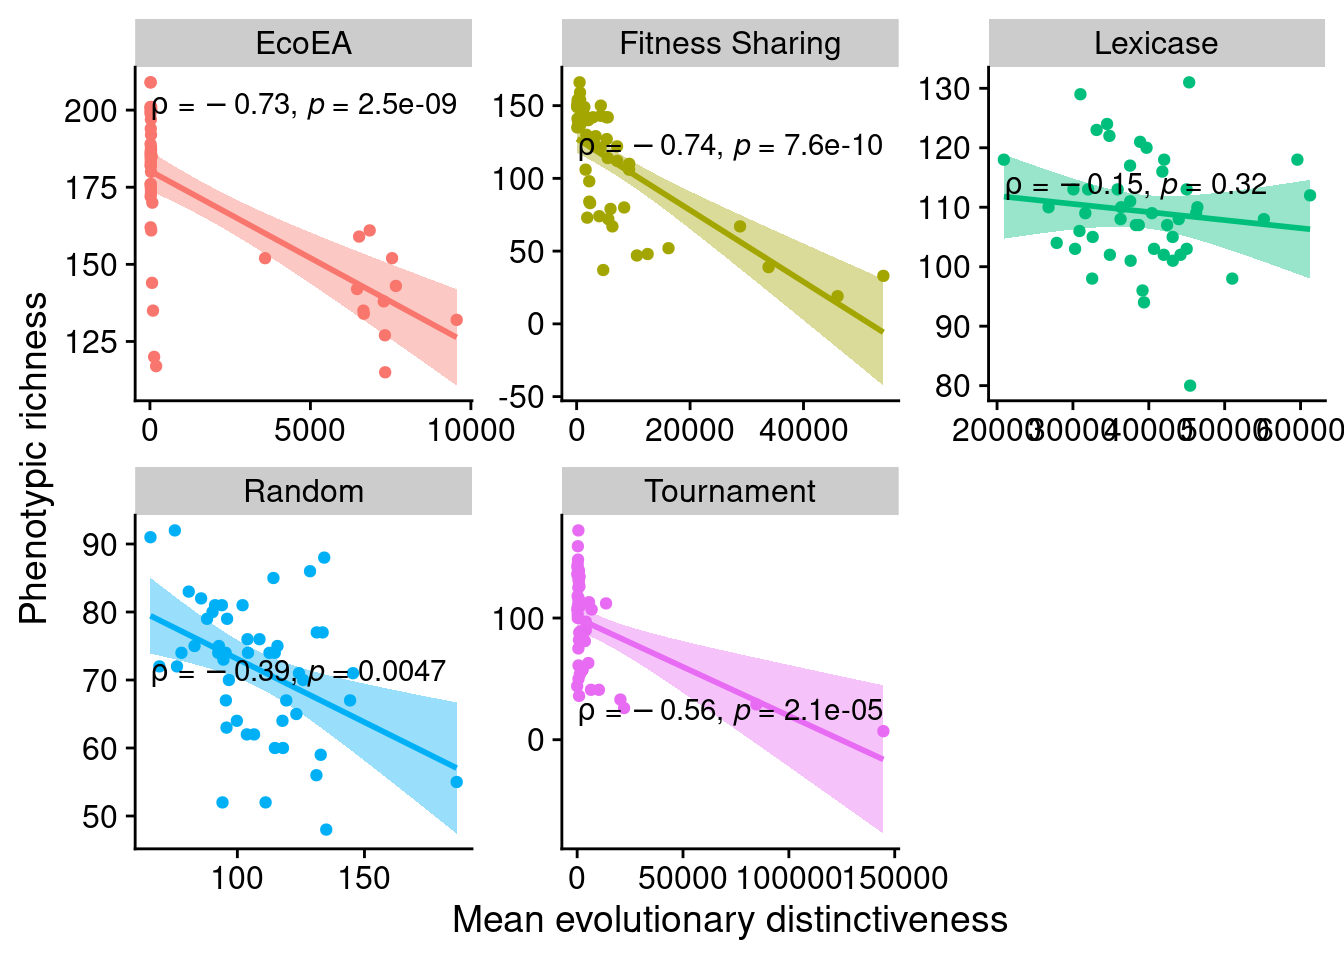
\includegraphics{phylodiversity-in-EC-supplement_files/figure-latex/phen_vs_phylo_richness_med-1.pdf}

These are mostly significant, but negative. That's interesting and worthy of further exploration (but it's a little beyond the scope of this analysis).

\hypertarget{phenotypic-shannon-diversity-vs.mean-pairwise-distance}{%
\subsection{Phenotypic shannon diversity vs.~mean pairwise distance}\label{phenotypic-shannon-diversity-vs.mean-pairwise-distance}}

\begin{Shaded}
\begin{Highlighting}[]
\KeywordTok{ggplot}\NormalTok{(}
\NormalTok{    data }\OperatorTok\StringTok{ }\KeywordTok{filter}\NormalTok{(gen}\OperatorTok{==}\DecValTok{500000}\NormalTok{),}
    \KeywordTok{aes}\NormalTok{(}
        \DataTypeTok{y=}\NormalTok{phen_diversity,}
        \DataTypeTok{x=}\NormalTok{mean_phenotype_pairwise_distance,}
        \DataTypeTok{color=}\NormalTok{selection_name,}
        \DataTypeTok{fill=}\NormalTok{selection_name}
\NormalTok{    )}
\NormalTok{  ) }\OperatorTok{+}
\StringTok{  }\KeywordTok{geom_point}\NormalTok{() }\OperatorTok{+}
\StringTok{    }\KeywordTok{scale_y_continuous}\NormalTok{(}
        \DataTypeTok{name=}\StringTok{"Phenotypic shannon diversity"}
\NormalTok{  ) }\OperatorTok{+}
\StringTok{  }\KeywordTok{scale_x_continuous}\NormalTok{(}
        \DataTypeTok{name=}\StringTok{"Mean pairwise distance"}\NormalTok{,}
        \DataTypeTok{breaks =} \KeywordTok{breaks_extended}\NormalTok{(}\DecValTok{4}\NormalTok{)}
\NormalTok{  ) }\OperatorTok{+}\StringTok{ }
\StringTok{  }\KeywordTok{facet_wrap}\NormalTok{(}
      \OperatorTok{~}\NormalTok{selection_name, }\DataTypeTok{scales=}\StringTok{"free"}
\NormalTok{  ) }\OperatorTok{+}\StringTok{ }
\StringTok{  }\KeywordTok{stat_smooth}\NormalTok{(}
    \DataTypeTok{method=}\StringTok{"lm"}
\NormalTok{  ) }\OperatorTok{+}\StringTok{ }
\StringTok{  }\KeywordTok{stat_cor}\NormalTok{(}
    \DataTypeTok{method=}\StringTok{"spearman"}\NormalTok{, }\DataTypeTok{cor.coef.name =} \StringTok{"rho"}\NormalTok{, }\DataTypeTok{color=}\StringTok{"black"}
\NormalTok{  ) }\OperatorTok{+}
\StringTok{  }\KeywordTok{theme}\NormalTok{(}\DataTypeTok{legend.position =} \StringTok{"none"}\NormalTok{)}
\end{Highlighting}
\end{Shaded}

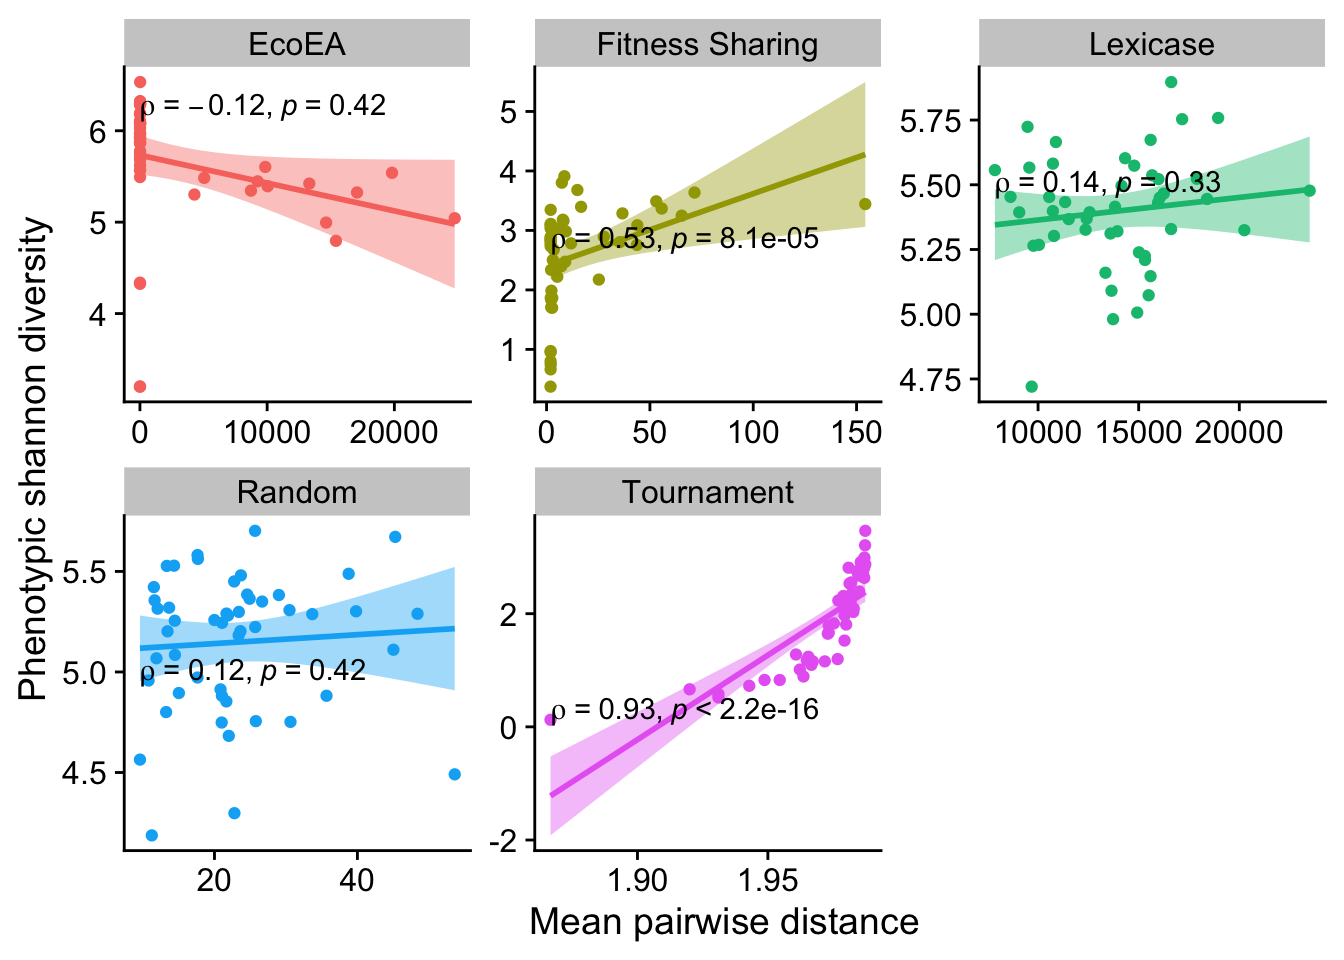
\includegraphics{phylodiversity-in-EC-supplement_files/figure-latex/phen_vs_phylo_shannon_mpd-1.pdf}

Again, these are mostly not significant (although fitness sharing notably now is).

\hypertarget{phenotypic-shannon-diversity-vs.mean-evolutionary-distinctiveness}{%
\subsection{Phenotypic shannon diversity vs.~mean evolutionary distinctiveness}\label{phenotypic-shannon-diversity-vs.mean-evolutionary-distinctiveness}}

\begin{Shaded}
\begin{Highlighting}[]
\KeywordTok{ggplot}\NormalTok{(}
\NormalTok{    data }\OperatorTok\StringTok{ }\KeywordTok{filter}\NormalTok{(gen}\OperatorTok{==}\DecValTok{500000}\NormalTok{),}
    \KeywordTok{aes}\NormalTok{(}
        \DataTypeTok{y=}\NormalTok{phen_diversity,}
        \DataTypeTok{x=}\NormalTok{mean_phenotype_evolutionary_distinctiveness,}
        \DataTypeTok{color=}\NormalTok{selection_name,}
        \DataTypeTok{fill=}\NormalTok{selection_name}
\NormalTok{    )}
\NormalTok{  ) }\OperatorTok{+}
\StringTok{  }\KeywordTok{geom_point}\NormalTok{() }\OperatorTok{+}
\StringTok{    }\KeywordTok{scale_y_continuous}\NormalTok{(}
        \DataTypeTok{name=}\StringTok{"Phenotypic shannon diversity"}
\NormalTok{  ) }\OperatorTok{+}
\StringTok{  }\KeywordTok{scale_x_continuous}\NormalTok{(}
        \DataTypeTok{name=}\StringTok{"Mean evolutionary distinctiveness"}\NormalTok{,}
        \DataTypeTok{breaks =} \KeywordTok{breaks_extended}\NormalTok{(}\DecValTok{4}\NormalTok{)}
\NormalTok{  ) }\OperatorTok{+}\StringTok{ }
\StringTok{  }\KeywordTok{facet_wrap}\NormalTok{(}
      \OperatorTok{~}\NormalTok{selection_name, }\DataTypeTok{scales=}\StringTok{"free"}
\NormalTok{  ) }\OperatorTok{+}\StringTok{ }
\StringTok{  }\KeywordTok{stat_smooth}\NormalTok{(}
    \DataTypeTok{method=}\StringTok{"lm"}
\NormalTok{  ) }\OperatorTok{+}\StringTok{ }
\StringTok{  }\KeywordTok{stat_cor}\NormalTok{(}
    \DataTypeTok{method=}\StringTok{"spearman"}\NormalTok{, }\DataTypeTok{cor.coef.name =} \StringTok{"rho"}\NormalTok{, }\DataTypeTok{color=}\StringTok{"black"}
\NormalTok{  ) }\OperatorTok{+}
\StringTok{  }\KeywordTok{theme}\NormalTok{(}\DataTypeTok{legend.position =} \StringTok{"none"}\NormalTok{)}
\end{Highlighting}
\end{Shaded}

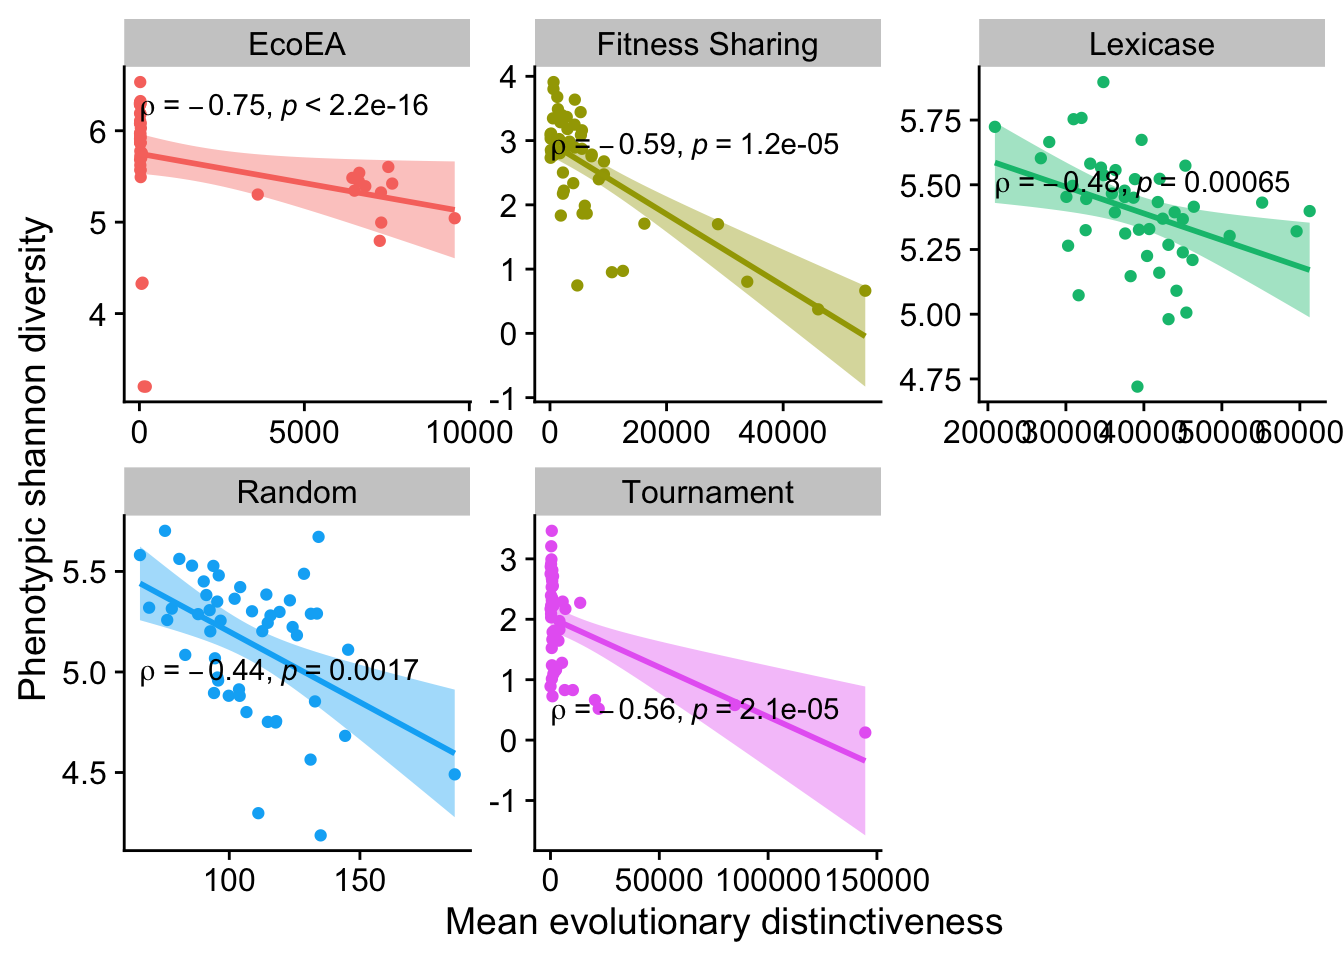
\includegraphics{phylodiversity-in-EC-supplement_files/figure-latex/phen_vs_phylo_shannon_med-1.pdf}

Again, all significant but negative. From this we can conclude that there is substantially more overlap between the information captured by phenotypic diversity and mean evolutionary disinctiveness than between phenotypic diversity metrics and mean pairwise distance. However, thus information has wildly different implications in the two contexts. Moreover, the long term trends are still very different. Thus, we still feel confident in saying that these metrics are meaningfully different. More investigation here may be worthwhile in the future.

Overall, based on these end of time analyses and qualitative comparison of the temporal graphs, we conclude that phenotypic and phylogenetic diversity are meaningfully different from each other in the context of evolutionary computation. In retrospect, this finding may seem obvious. However a lot of people tend to assume that these two classes of diversity are closely related.

\hypertarget{relationship-between-diversity-and-success}{%
\section{Relationship between diversity and success}\label{relationship-between-diversity-and-success}}

At last, we can finally assess whether diversity leads to actually solving problems! We start out by looking at correlations between diversity success across a few different time points,
although we ultimately conclude that this approach is not particularly informative.

\hypertarget{very-early-in-run}{%
\subsection{Very early in run}\label{very-early-in-run}}

\hypertarget{mean-pairwise-distance-2}{%
\subsubsection{Mean pairwise distance}\label{mean-pairwise-distance-2}}

\begin{Shaded}
\begin{Highlighting}[]
\KeywordTok{ggplot}\NormalTok{(}
\NormalTok{    data }\OperatorTok\StringTok{ }\KeywordTok{filter}\NormalTok{(gen}\OperatorTok{==}\DecValTok{25000}\NormalTok{),}
    \KeywordTok{aes}\NormalTok{(}
        \DataTypeTok{y=}\NormalTok{elite_trait_avg,}
        \DataTypeTok{x=}\NormalTok{mean_phenotype_pairwise_distance,}
        \DataTypeTok{color=}\NormalTok{selection_name,}
        \DataTypeTok{fill=}\NormalTok{selection_name}
\NormalTok{    )}
\NormalTok{  ) }\OperatorTok{+}
\StringTok{  }\KeywordTok{geom_point}\NormalTok{() }\OperatorTok{+}
\StringTok{    }\KeywordTok{scale_y_continuous}\NormalTok{(}
        \DataTypeTok{name=}\StringTok{"Average trait performance"}
\NormalTok{  ) }\OperatorTok{+}
\StringTok{  }\KeywordTok{scale_x_continuous}\NormalTok{(}
        \DataTypeTok{name=}\StringTok{"Mean pairwise distance"}
\NormalTok{  ) }\OperatorTok{+}\StringTok{ }
\StringTok{  }\KeywordTok{facet_wrap}\NormalTok{(}
      \OperatorTok{~}\NormalTok{selection_name, }\DataTypeTok{scales=}\StringTok{"free"}
\NormalTok{  ) }\OperatorTok{+}\StringTok{ }
\StringTok{  }\KeywordTok{stat_smooth}\NormalTok{(}
    \DataTypeTok{method=}\StringTok{"lm"}
\NormalTok{  ) }\OperatorTok{+}\StringTok{ }
\StringTok{  }\KeywordTok{stat_cor}\NormalTok{(}
    \DataTypeTok{method=}\StringTok{"spearman"}\NormalTok{, }\DataTypeTok{cor.coef.name =} \StringTok{"rho"}\NormalTok{, }\DataTypeTok{color=}\StringTok{"black"}
\NormalTok{  ) }\OperatorTok{+}
\StringTok{  }\KeywordTok{theme}\NormalTok{(}\DataTypeTok{legend.position =} \StringTok{"none"}\NormalTok{)}
\end{Highlighting}
\end{Shaded}

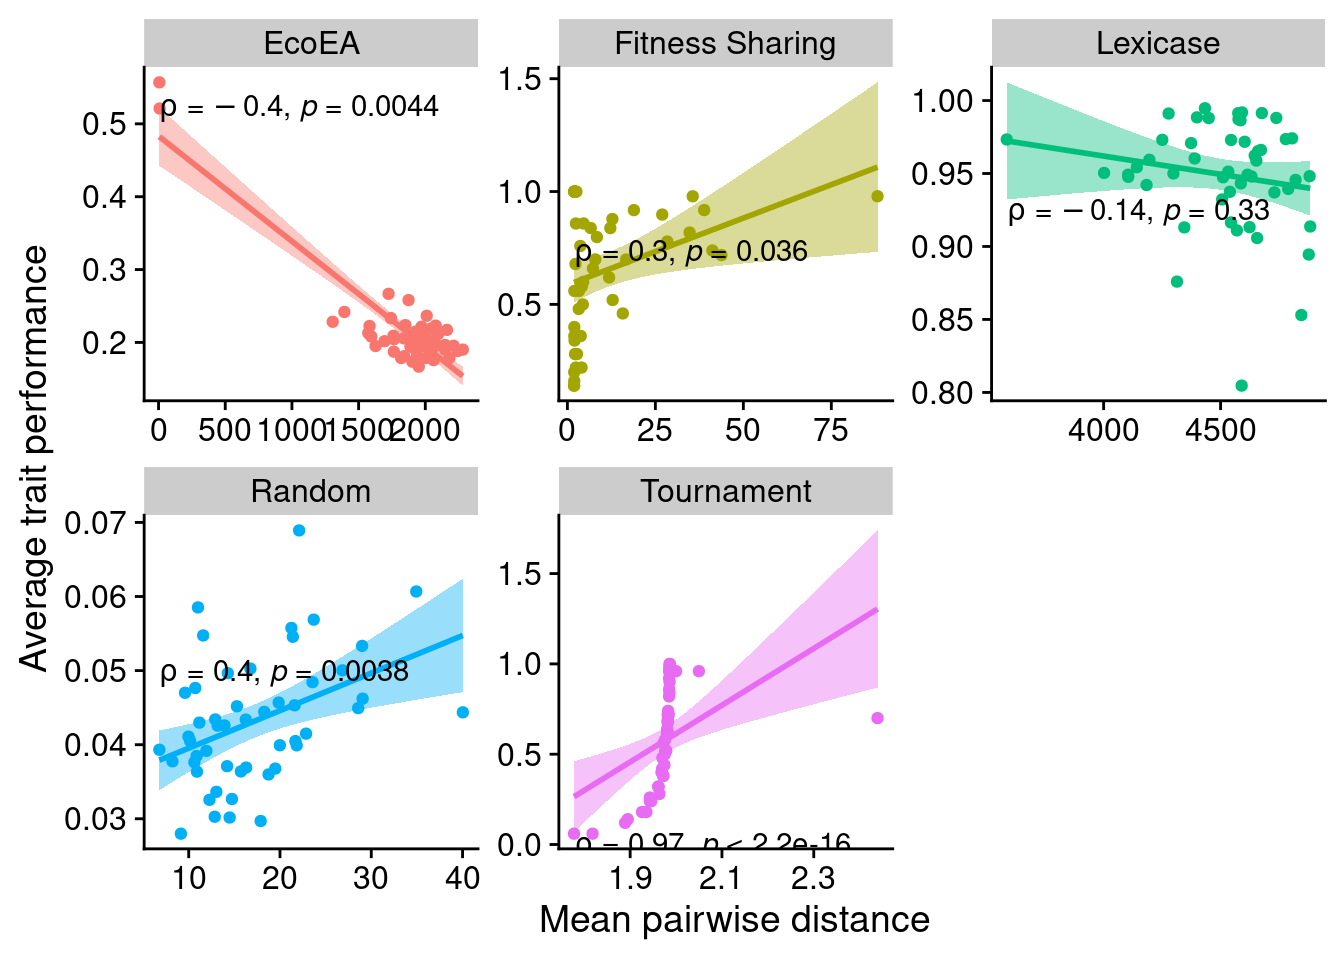
\includegraphics{phylodiversity-in-EC-supplement_files/figure-latex/phylogeny_vs_performance_very_early-1.pdf}

\hypertarget{mean-evolutionary-distinctiveness-2}{%
\subsubsection{Mean evolutionary distinctiveness}\label{mean-evolutionary-distinctiveness-2}}

\begin{Shaded}
\begin{Highlighting}[]
\KeywordTok{ggplot}\NormalTok{(}
\NormalTok{    data }\OperatorTok\StringTok{ }\KeywordTok{filter}\NormalTok{(gen}\OperatorTok{==}\DecValTok{25000}\NormalTok{),}
    \KeywordTok{aes}\NormalTok{(}
        \DataTypeTok{y=}\NormalTok{elite_trait_avg,}
        \DataTypeTok{x=}\NormalTok{mean_phenotype_evolutionary_distinctiveness,}
        \DataTypeTok{color=}\NormalTok{selection_name,}
        \DataTypeTok{fill=}\NormalTok{selection_name}
\NormalTok{    )}
\NormalTok{  ) }\OperatorTok{+}
\StringTok{  }\KeywordTok{geom_point}\NormalTok{() }\OperatorTok{+}
\StringTok{    }\KeywordTok{scale_y_continuous}\NormalTok{(}
        \DataTypeTok{name=}\StringTok{"Average trait performance"}
\NormalTok{  ) }\OperatorTok{+}
\StringTok{  }\KeywordTok{scale_x_continuous}\NormalTok{(}
        \DataTypeTok{name=}\StringTok{"Mean evolutionary distinctiveness"}
\NormalTok{  ) }\OperatorTok{+}\StringTok{ }
\StringTok{  }\KeywordTok{facet_wrap}\NormalTok{(}
      \OperatorTok{~}\NormalTok{selection_name, }\DataTypeTok{scales=}\StringTok{"free"}
\NormalTok{  ) }\OperatorTok{+}\StringTok{ }
\StringTok{  }\KeywordTok{stat_smooth}\NormalTok{(}
    \DataTypeTok{method=}\StringTok{"lm"}
\NormalTok{  ) }\OperatorTok{+}\StringTok{ }
\StringTok{  }\KeywordTok{stat_cor}\NormalTok{(}
    \DataTypeTok{method=}\StringTok{"spearman"}\NormalTok{, }\DataTypeTok{cor.coef.name =} \StringTok{"rho"}\NormalTok{, }\DataTypeTok{color=}\StringTok{"black"}
\NormalTok{  ) }\OperatorTok{+}
\StringTok{  }\KeywordTok{theme}\NormalTok{(}\DataTypeTok{legend.position =} \StringTok{"none"}\NormalTok{)}
\end{Highlighting}
\end{Shaded}

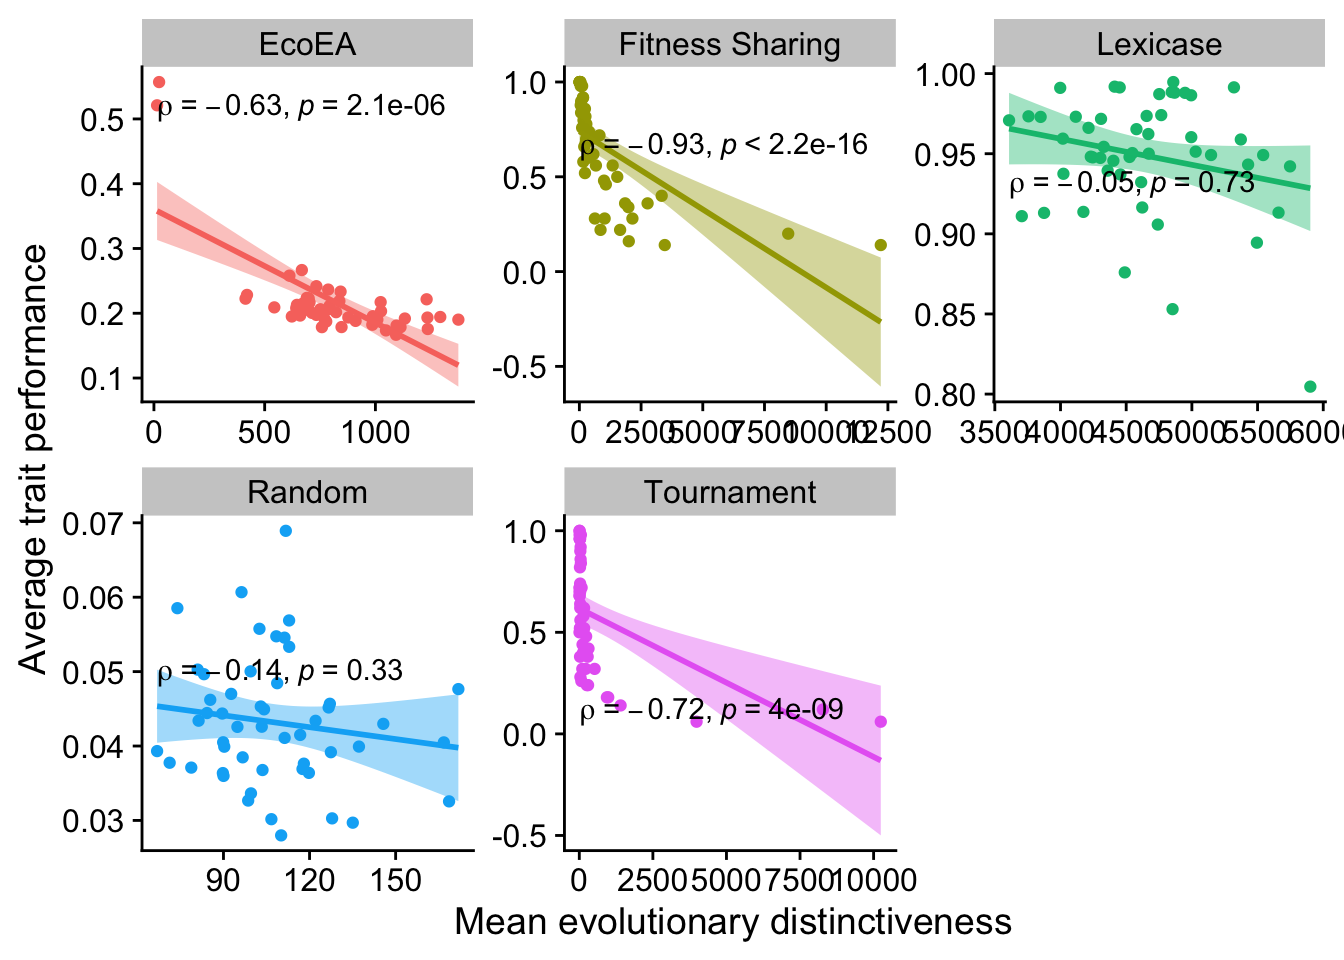
\includegraphics{phylodiversity-in-EC-supplement_files/figure-latex/phylogeny_vs_performance_very_early_med-1.pdf}

\hypertarget{richness-2}{%
\subsubsection{Richness}\label{richness-2}}

\begin{Shaded}
\begin{Highlighting}[]
\KeywordTok{ggplot}\NormalTok{(}
\NormalTok{    data }\OperatorTok\StringTok{ }\KeywordTok{filter}\NormalTok{(gen}\OperatorTok{==}\DecValTok{25000}\NormalTok{),}
    \KeywordTok{aes}\NormalTok{(}
        \DataTypeTok{y=}\NormalTok{elite_trait_avg,}
        \DataTypeTok{x=}\NormalTok{phen_num_taxa,}
        \DataTypeTok{color=}\NormalTok{selection_name,}
        \DataTypeTok{fill=}\NormalTok{selection_name}
\NormalTok{    )}
\NormalTok{  ) }\OperatorTok{+}
\StringTok{  }\KeywordTok{geom_point}\NormalTok{() }\OperatorTok{+}
\StringTok{    }\KeywordTok{scale_y_continuous}\NormalTok{(}
        \DataTypeTok{name=}\StringTok{"Average trait performance"}
\NormalTok{  ) }\OperatorTok{+}
\StringTok{  }\KeywordTok{scale_x_continuous}\NormalTok{(}
        \DataTypeTok{name=}\StringTok{"Phenotypic richness"}
\NormalTok{  ) }\OperatorTok{+}\StringTok{ }
\StringTok{  }\KeywordTok{facet_wrap}\NormalTok{(}
      \OperatorTok{~}\NormalTok{selection_name, }\DataTypeTok{scales=}\StringTok{"free"}
\NormalTok{  ) }\OperatorTok{+}\StringTok{ }
\StringTok{  }\KeywordTok{stat_smooth}\NormalTok{(}
    \DataTypeTok{method=}\StringTok{"lm"}
\NormalTok{  ) }\OperatorTok{+}\StringTok{ }
\StringTok{  }\KeywordTok{stat_cor}\NormalTok{(}
    \DataTypeTok{method=}\StringTok{"spearman"}\NormalTok{, }\DataTypeTok{cor.coef.name =} \StringTok{"rho"}\NormalTok{, }\DataTypeTok{color=}\StringTok{"black"}
\NormalTok{  ) }\OperatorTok{+}
\StringTok{  }\KeywordTok{theme}\NormalTok{(}\DataTypeTok{legend.position =} \StringTok{"none"}\NormalTok{)}
\end{Highlighting}
\end{Shaded}

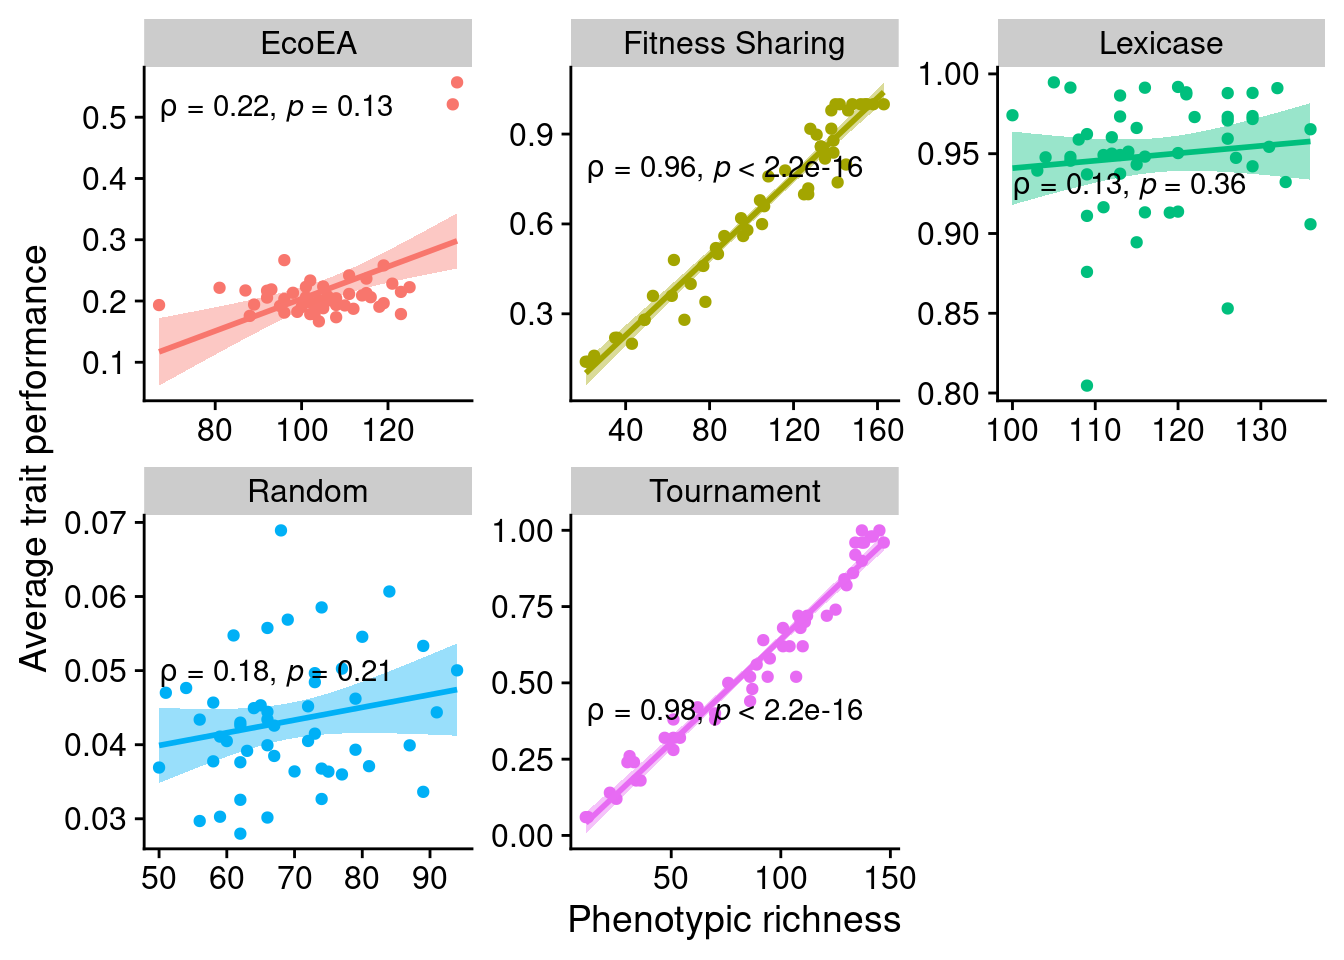
\includegraphics{phylodiversity-in-EC-supplement_files/figure-latex/richness_vs_performance_very_early-1.pdf}

\hypertarget{shannon-diversity-2}{%
\subsubsection{Shannon diversity}\label{shannon-diversity-2}}

\begin{Shaded}
\begin{Highlighting}[]
\KeywordTok{ggplot}\NormalTok{(}
\NormalTok{    data }\OperatorTok\StringTok{ }\KeywordTok{filter}\NormalTok{(gen}\OperatorTok{==}\DecValTok{25000}\NormalTok{),}
    \KeywordTok{aes}\NormalTok{(}
        \DataTypeTok{y=}\NormalTok{elite_trait_avg,}
        \DataTypeTok{x=}\NormalTok{phen_diversity,}
        \DataTypeTok{color=}\NormalTok{selection_name,}
        \DataTypeTok{fill=}\NormalTok{selection_name}
\NormalTok{    )}
\NormalTok{  ) }\OperatorTok{+}
\StringTok{  }\KeywordTok{geom_point}\NormalTok{() }\OperatorTok{+}
\StringTok{    }\KeywordTok{scale_y_continuous}\NormalTok{(}
        \DataTypeTok{name=}\StringTok{"Average trait performance"}
\NormalTok{  ) }\OperatorTok{+}
\StringTok{  }\KeywordTok{scale_x_continuous}\NormalTok{(}
        \DataTypeTok{name=}\StringTok{"Phenotypic Shannon diversity"}
\NormalTok{  ) }\OperatorTok{+}\StringTok{ }
\StringTok{  }\KeywordTok{facet_wrap}\NormalTok{(}
      \OperatorTok{~}\NormalTok{selection_name, }\DataTypeTok{scales=}\StringTok{"free"}
\NormalTok{  ) }\OperatorTok{+}\StringTok{ }
\StringTok{  }\KeywordTok{stat_smooth}\NormalTok{(}
    \DataTypeTok{method=}\StringTok{"lm"}
\NormalTok{  ) }\OperatorTok{+}\StringTok{ }
\StringTok{  }\KeywordTok{stat_cor}\NormalTok{(}
    \DataTypeTok{method=}\StringTok{"spearman"}\NormalTok{, }\DataTypeTok{cor.coef.name =} \StringTok{"rho"}\NormalTok{, }\DataTypeTok{color=}\StringTok{"black"}
\NormalTok{  ) }\OperatorTok{+}
\StringTok{  }\KeywordTok{theme}\NormalTok{(}\DataTypeTok{legend.position =} \StringTok{"none"}\NormalTok{)}
\end{Highlighting}
\end{Shaded}

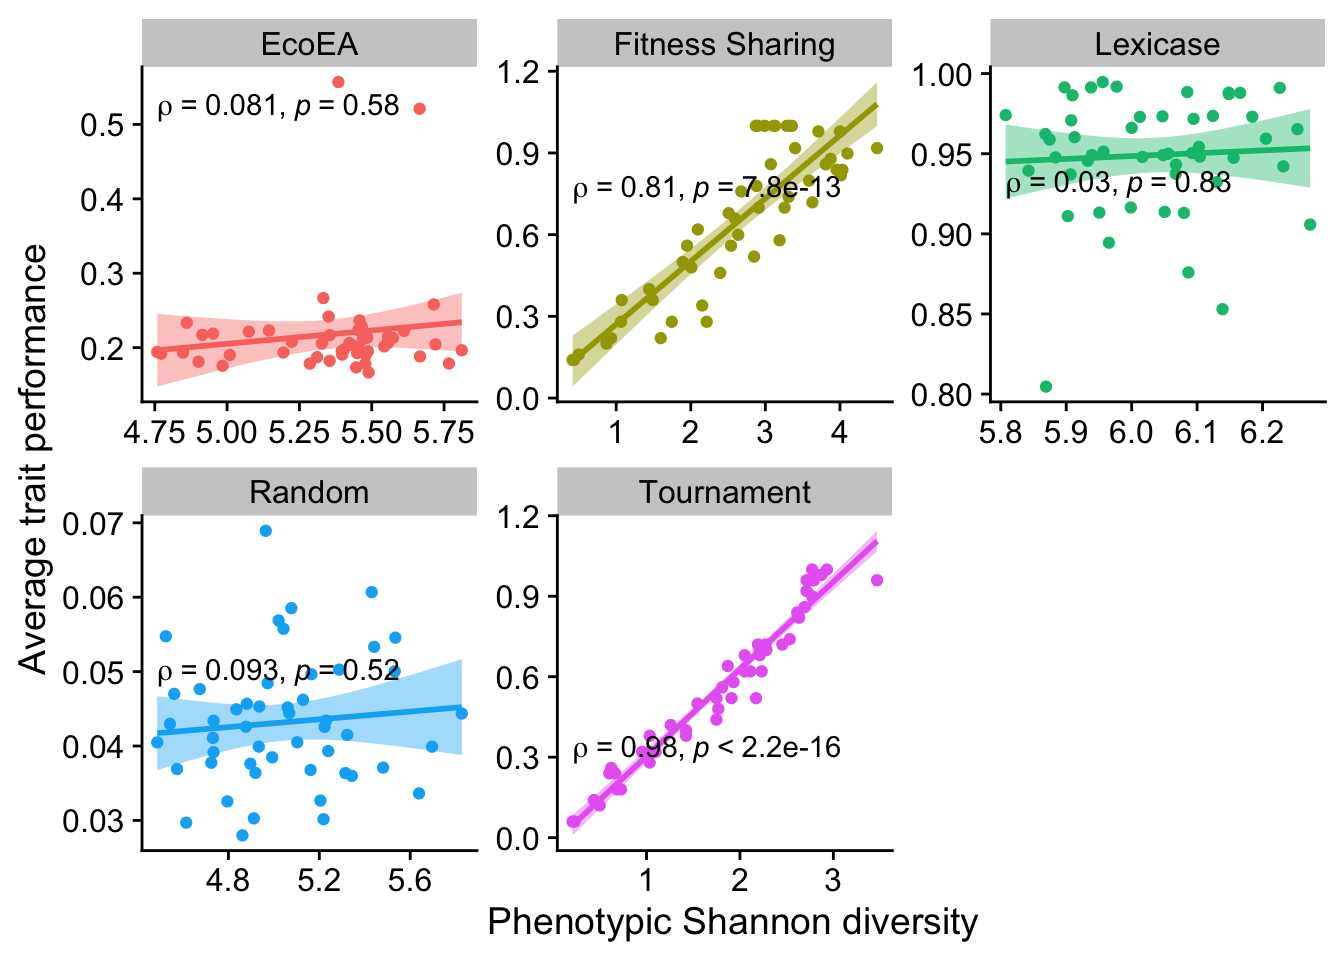
\includegraphics{phylodiversity-in-EC-supplement_files/figure-latex/shannon_vs_performance_very_early-1.pdf}

\hypertarget{middle-of-run}{%
\subsection{Middle of run}\label{middle-of-run}}

\hypertarget{mean-pairwise-distance-3}{%
\subsubsection{Mean pairwise distance}\label{mean-pairwise-distance-3}}

\begin{Shaded}
\begin{Highlighting}[]
\KeywordTok{ggplot}\NormalTok{(}
\NormalTok{    data }\OperatorTok\StringTok{ }\KeywordTok{filter}\NormalTok{(gen}\OperatorTok{==}\DecValTok{50000}\NormalTok{),}
    \KeywordTok{aes}\NormalTok{(}
        \DataTypeTok{y=}\NormalTok{elite_trait_avg,}
        \DataTypeTok{x=}\NormalTok{mean_phenotype_pairwise_distance,}
        \DataTypeTok{color=}\NormalTok{selection_name,}
        \DataTypeTok{fill=}\NormalTok{selection_name}
\NormalTok{    )}
\NormalTok{  ) }\OperatorTok{+}
\StringTok{  }\KeywordTok{geom_point}\NormalTok{() }\OperatorTok{+}
\StringTok{    }\KeywordTok{scale_y_continuous}\NormalTok{(}
        \DataTypeTok{name=}\StringTok{"Average trait performance"}
\NormalTok{  ) }\OperatorTok{+}
\StringTok{  }\KeywordTok{scale_x_continuous}\NormalTok{(}
        \DataTypeTok{name=}\StringTok{"Mean pairwise distance"}
\NormalTok{  ) }\OperatorTok{+}\StringTok{ }
\StringTok{  }\KeywordTok{facet_wrap}\NormalTok{(}
      \OperatorTok{~}\NormalTok{selection_name, }\DataTypeTok{scales=}\StringTok{"free"}
\NormalTok{  ) }\OperatorTok{+}\StringTok{ }
\StringTok{  }\KeywordTok{stat_smooth}\NormalTok{(}
    \DataTypeTok{method=}\StringTok{"lm"}
\NormalTok{  ) }\OperatorTok{+}\StringTok{ }
\StringTok{  }\KeywordTok{stat_cor}\NormalTok{(}
    \DataTypeTok{method=}\StringTok{"spearman"}\NormalTok{, }\DataTypeTok{cor.coef.name =} \StringTok{"rho"}\NormalTok{, }\DataTypeTok{color=}\StringTok{"black"}
\NormalTok{  ) }\OperatorTok{+}
\StringTok{  }\KeywordTok{theme}\NormalTok{(}\DataTypeTok{legend.position =} \StringTok{"none"}\NormalTok{)}
\end{Highlighting}
\end{Shaded}

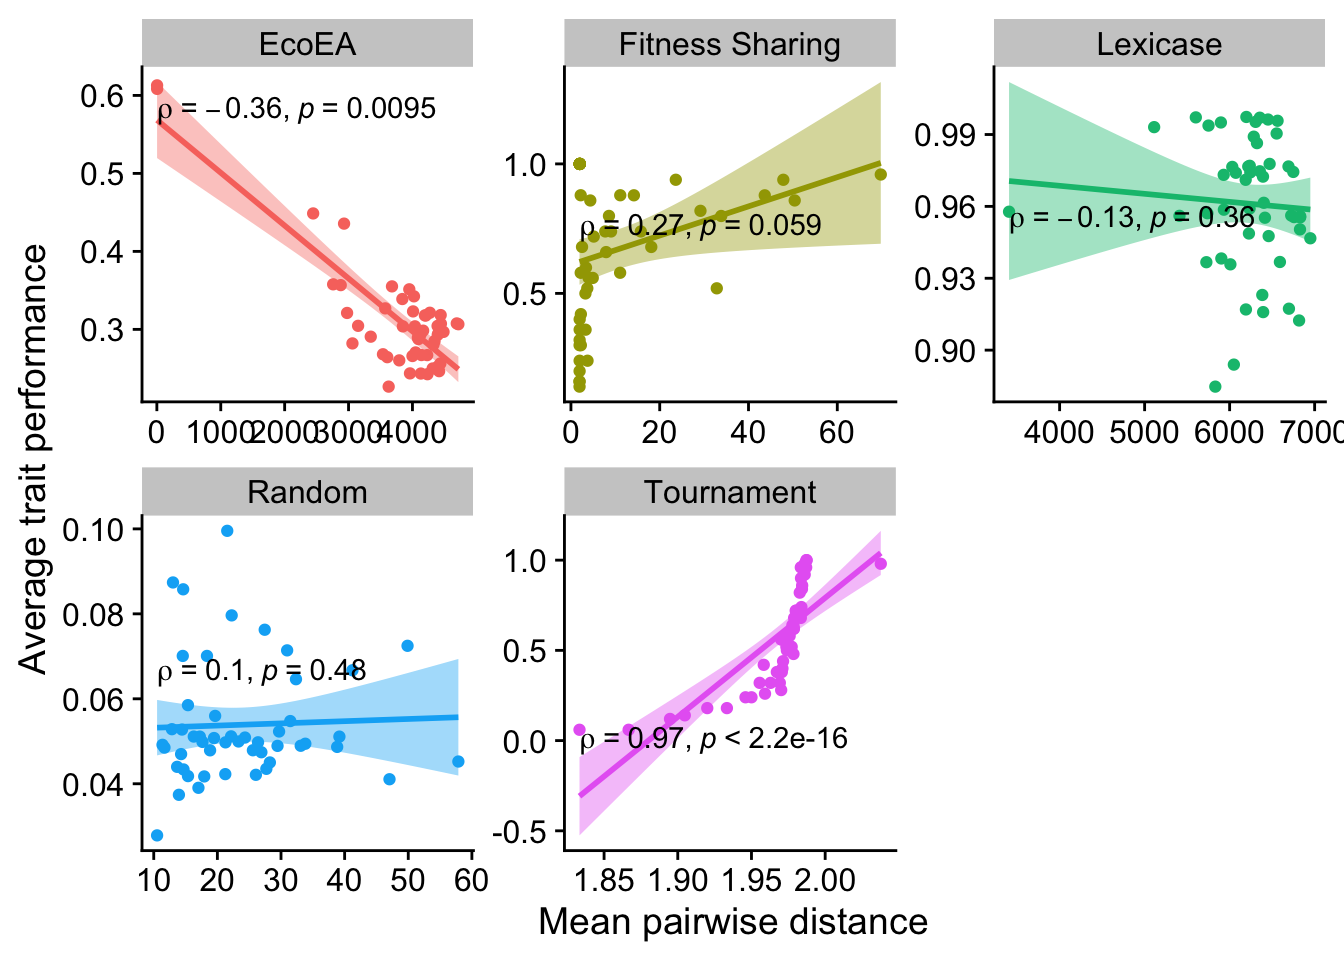
\includegraphics{phylodiversity-in-EC-supplement_files/figure-latex/phylogeny_vs_performance_early-1.pdf}

\hypertarget{mean-evolutionary-distinctiveness-3}{%
\subsubsection{Mean evolutionary distinctiveness}\label{mean-evolutionary-distinctiveness-3}}

\begin{Shaded}
\begin{Highlighting}[]
\KeywordTok{ggplot}\NormalTok{(}
\NormalTok{    data }\OperatorTok\StringTok{ }\KeywordTok{filter}\NormalTok{(gen}\OperatorTok{==}\DecValTok{50000}\NormalTok{),}
    \KeywordTok{aes}\NormalTok{(}
        \DataTypeTok{y=}\NormalTok{elite_trait_avg,}
        \DataTypeTok{x=}\NormalTok{mean_phenotype_evolutionary_distinctiveness,}
        \DataTypeTok{color=}\NormalTok{selection_name,}
        \DataTypeTok{fill=}\NormalTok{selection_name}
\NormalTok{    )}
\NormalTok{  ) }\OperatorTok{+}
\StringTok{  }\KeywordTok{geom_point}\NormalTok{() }\OperatorTok{+}
\StringTok{    }\KeywordTok{scale_y_continuous}\NormalTok{(}
        \DataTypeTok{name=}\StringTok{"Average trait performance"}
\NormalTok{  ) }\OperatorTok{+}
\StringTok{  }\KeywordTok{scale_x_continuous}\NormalTok{(}
        \DataTypeTok{name=}\StringTok{"Mean evolutionary distinctiveness"}
\NormalTok{  ) }\OperatorTok{+}\StringTok{ }
\StringTok{  }\KeywordTok{facet_wrap}\NormalTok{(}
      \OperatorTok{~}\NormalTok{selection_name, }\DataTypeTok{scales=}\StringTok{"free"}
\NormalTok{  ) }\OperatorTok{+}\StringTok{ }
\StringTok{  }\KeywordTok{stat_smooth}\NormalTok{(}
    \DataTypeTok{method=}\StringTok{"lm"}
\NormalTok{  ) }\OperatorTok{+}\StringTok{ }
\StringTok{  }\KeywordTok{stat_cor}\NormalTok{(}
    \DataTypeTok{method=}\StringTok{"spearman"}\NormalTok{, }\DataTypeTok{cor.coef.name =} \StringTok{"rho"}\NormalTok{, }\DataTypeTok{color=}\StringTok{"black"}
\NormalTok{  ) }\OperatorTok{+}
\StringTok{  }\KeywordTok{theme}\NormalTok{(}\DataTypeTok{legend.position =} \StringTok{"none"}\NormalTok{)}
\end{Highlighting}
\end{Shaded}

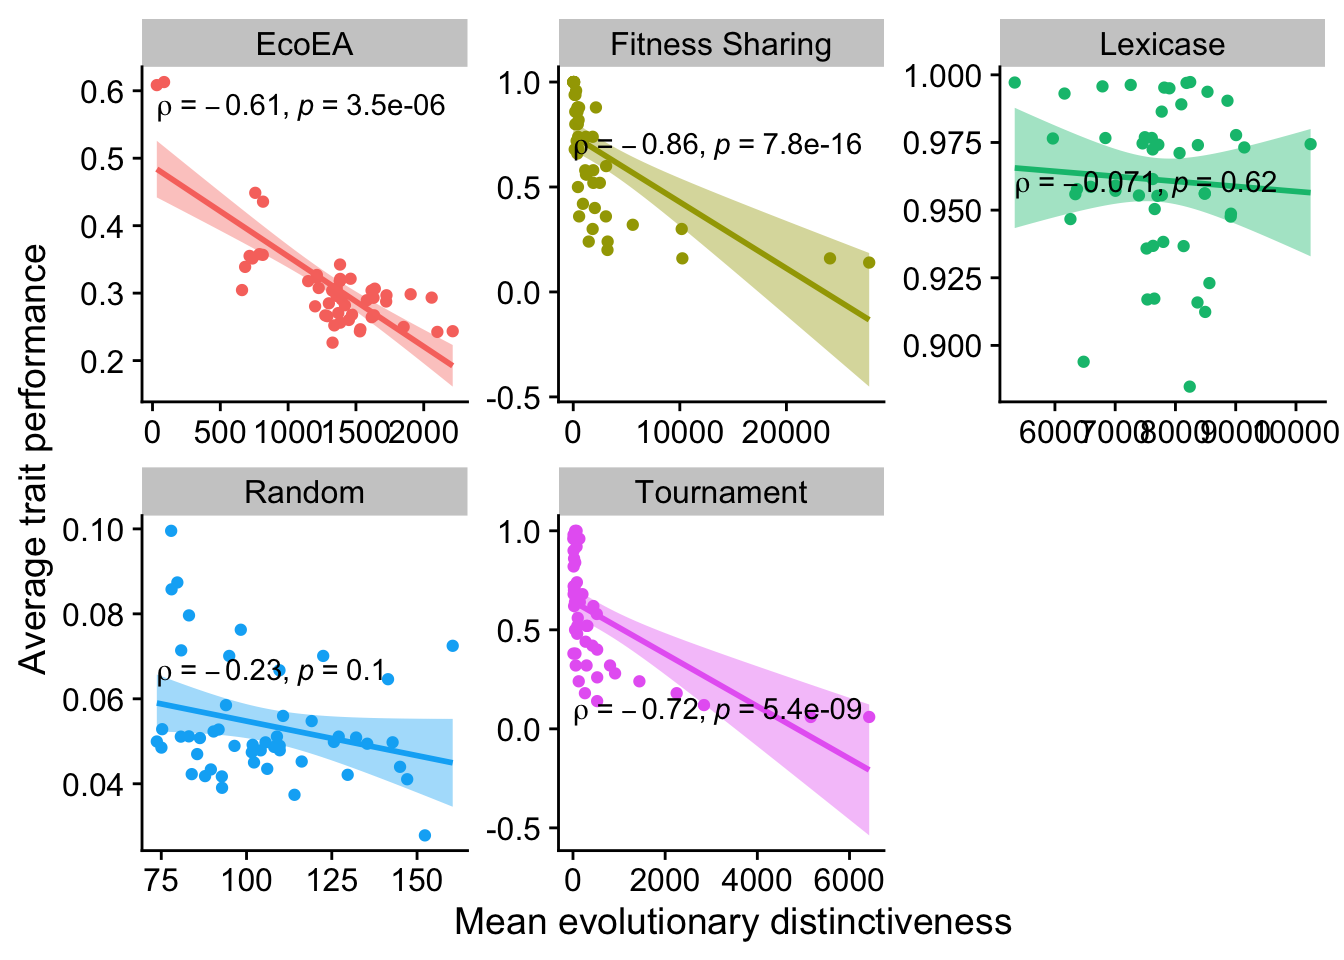
\includegraphics{phylodiversity-in-EC-supplement_files/figure-latex/med_vs_performance_early-1.pdf}

\hypertarget{richness-3}{%
\subsubsection{Richness}\label{richness-3}}

\begin{Shaded}
\begin{Highlighting}[]
\KeywordTok{ggplot}\NormalTok{(}
\NormalTok{    data }\OperatorTok\StringTok{ }\KeywordTok{filter}\NormalTok{(gen}\OperatorTok{==}\DecValTok{50000}\NormalTok{),}
    \KeywordTok{aes}\NormalTok{(}
        \DataTypeTok{y=}\NormalTok{elite_trait_avg,}
        \DataTypeTok{x=}\NormalTok{phen_num_taxa,}
        \DataTypeTok{color=}\NormalTok{selection_name,}
        \DataTypeTok{fill=}\NormalTok{selection_name}
\NormalTok{    )}
\NormalTok{  ) }\OperatorTok{+}
\StringTok{  }\KeywordTok{geom_point}\NormalTok{() }\OperatorTok{+}
\StringTok{    }\KeywordTok{scale_y_continuous}\NormalTok{(}
        \DataTypeTok{name=}\StringTok{"Average trait performance"}
\NormalTok{  ) }\OperatorTok{+}
\StringTok{  }\KeywordTok{scale_x_continuous}\NormalTok{(}
        \DataTypeTok{name=}\StringTok{"Phenotypic richness"}
\NormalTok{  ) }\OperatorTok{+}\StringTok{ }
\StringTok{  }\KeywordTok{facet_wrap}\NormalTok{(}
      \OperatorTok{~}\NormalTok{selection_name, }\DataTypeTok{scales=}\StringTok{"free"}
\NormalTok{  ) }\OperatorTok{+}\StringTok{ }
\StringTok{  }\KeywordTok{stat_smooth}\NormalTok{(}
    \DataTypeTok{method=}\StringTok{"lm"}
\NormalTok{  ) }\OperatorTok{+}\StringTok{ }
\StringTok{  }\KeywordTok{stat_cor}\NormalTok{(}
    \DataTypeTok{method=}\StringTok{"spearman"}\NormalTok{, }\DataTypeTok{cor.coef.name =} \StringTok{"rho"}\NormalTok{, }\DataTypeTok{color=}\StringTok{"black"}
\NormalTok{  ) }\OperatorTok{+}
\StringTok{  }\KeywordTok{theme}\NormalTok{(}\DataTypeTok{legend.position =} \StringTok{"none"}\NormalTok{)}
\end{Highlighting}
\end{Shaded}

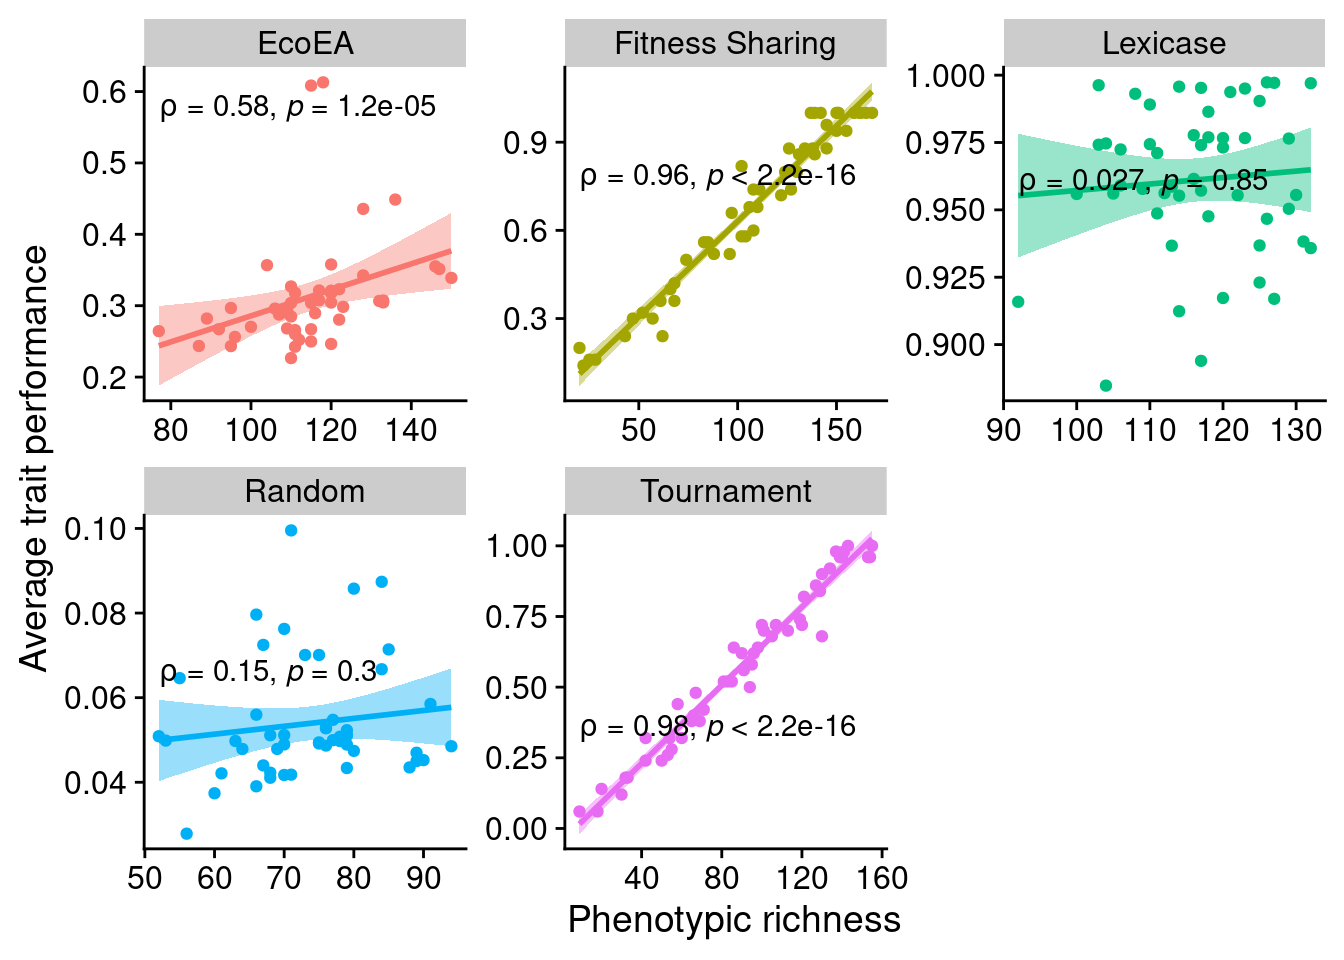
\includegraphics{phylodiversity-in-EC-supplement_files/figure-latex/richness_vs_performance_early-1.pdf}

\hypertarget{shannon-diversity-3}{%
\subsubsection{Shannon diversity}\label{shannon-diversity-3}}

\begin{Shaded}
\begin{Highlighting}[]
\KeywordTok{ggplot}\NormalTok{(}
\NormalTok{    data }\OperatorTok\StringTok{ }\KeywordTok{filter}\NormalTok{(gen}\OperatorTok{==}\DecValTok{50000}\NormalTok{),}
    \KeywordTok{aes}\NormalTok{(}
        \DataTypeTok{y=}\NormalTok{elite_trait_avg,}
        \DataTypeTok{x=}\NormalTok{phen_diversity,}
        \DataTypeTok{color=}\NormalTok{selection_name,}
        \DataTypeTok{fill=}\NormalTok{selection_name}
\NormalTok{    )}
\NormalTok{  ) }\OperatorTok{+}
\StringTok{  }\KeywordTok{geom_point}\NormalTok{() }\OperatorTok{+}
\StringTok{    }\KeywordTok{scale_y_continuous}\NormalTok{(}
        \DataTypeTok{name=}\StringTok{"Average trait performance"}
\NormalTok{  ) }\OperatorTok{+}
\StringTok{  }\KeywordTok{scale_x_continuous}\NormalTok{(}
        \DataTypeTok{name=}\StringTok{"Phenotypic Shannon diversity"}
\NormalTok{  ) }\OperatorTok{+}\StringTok{ }
\StringTok{  }\KeywordTok{facet_wrap}\NormalTok{(}
      \OperatorTok{~}\NormalTok{selection_name, }\DataTypeTok{scales=}\StringTok{"free"}
\NormalTok{  ) }\OperatorTok{+}\StringTok{ }
\StringTok{  }\KeywordTok{stat_smooth}\NormalTok{(}
    \DataTypeTok{method=}\StringTok{"lm"}
\NormalTok{  ) }\OperatorTok{+}\StringTok{ }
\StringTok{  }\KeywordTok{stat_cor}\NormalTok{(}
    \DataTypeTok{method=}\StringTok{"spearman"}\NormalTok{, }\DataTypeTok{cor.coef.name =} \StringTok{"rho"}\NormalTok{, }\DataTypeTok{color=}\StringTok{"black"}
\NormalTok{  ) }\OperatorTok{+}
\StringTok{  }\KeywordTok{theme}\NormalTok{(}\DataTypeTok{legend.position =} \StringTok{"none"}\NormalTok{)}
\end{Highlighting}
\end{Shaded}

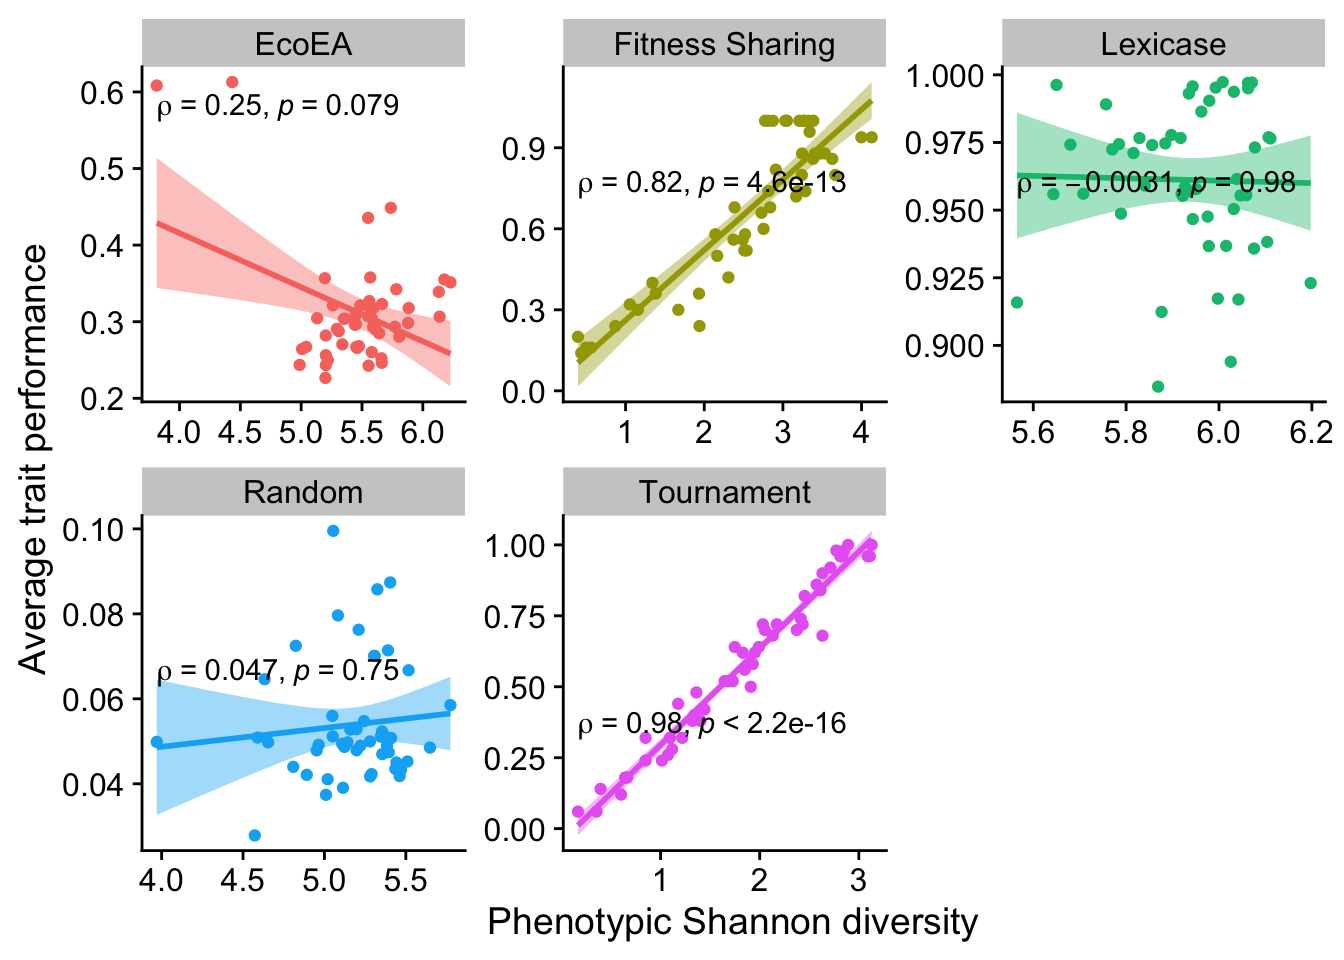
\includegraphics{phylodiversity-in-EC-supplement_files/figure-latex/shannon_vs_performance_early-1.pdf}

\hypertarget{end-of-run}{%
\subsection{End of run}\label{end-of-run}}

\hypertarget{mean-pairwise-distance-4}{%
\subsubsection{Mean pairwise distance}\label{mean-pairwise-distance-4}}

\begin{Shaded}
\begin{Highlighting}[]
\KeywordTok{ggplot}\NormalTok{(}
\NormalTok{    final_data,}
    \KeywordTok{aes}\NormalTok{(}
        \DataTypeTok{y=}\NormalTok{elite_trait_avg,}
        \DataTypeTok{x=}\NormalTok{mean_phenotype_pairwise_distance,}
        \DataTypeTok{color=}\NormalTok{selection_name,}
        \DataTypeTok{fill=}\NormalTok{selection_name}
\NormalTok{    )}
\NormalTok{  ) }\OperatorTok{+}
\StringTok{  }\KeywordTok{geom_point}\NormalTok{() }\OperatorTok{+}
\StringTok{    }\KeywordTok{scale_y_continuous}\NormalTok{(}
        \DataTypeTok{name=}\StringTok{"Average trait performance"}
\NormalTok{  ) }\OperatorTok{+}
\StringTok{  }\KeywordTok{scale_x_continuous}\NormalTok{(}
        \DataTypeTok{name=}\StringTok{"Mean pairwise distance"}
\NormalTok{  ) }\OperatorTok{+}\StringTok{ }
\StringTok{  }\KeywordTok{facet_wrap}\NormalTok{(}
      \OperatorTok{~}\NormalTok{selection_name, }\DataTypeTok{scales=}\StringTok{"free"}
\NormalTok{  ) }\OperatorTok{+}\StringTok{ }
\StringTok{  }\KeywordTok{stat_smooth}\NormalTok{(}
    \DataTypeTok{method=}\StringTok{"lm"}
\NormalTok{  ) }\OperatorTok{+}\StringTok{ }
\StringTok{  }\KeywordTok{stat_cor}\NormalTok{(}
    \DataTypeTok{method=}\StringTok{"spearman"}\NormalTok{, }\DataTypeTok{cor.coef.name =} \StringTok{"rho"}\NormalTok{, }\DataTypeTok{color=}\StringTok{"black"}
\NormalTok{  ) }\OperatorTok{+}
\StringTok{  }\KeywordTok{theme}\NormalTok{(}\DataTypeTok{legend.position =} \StringTok{"none"}\NormalTok{)}
\end{Highlighting}
\end{Shaded}

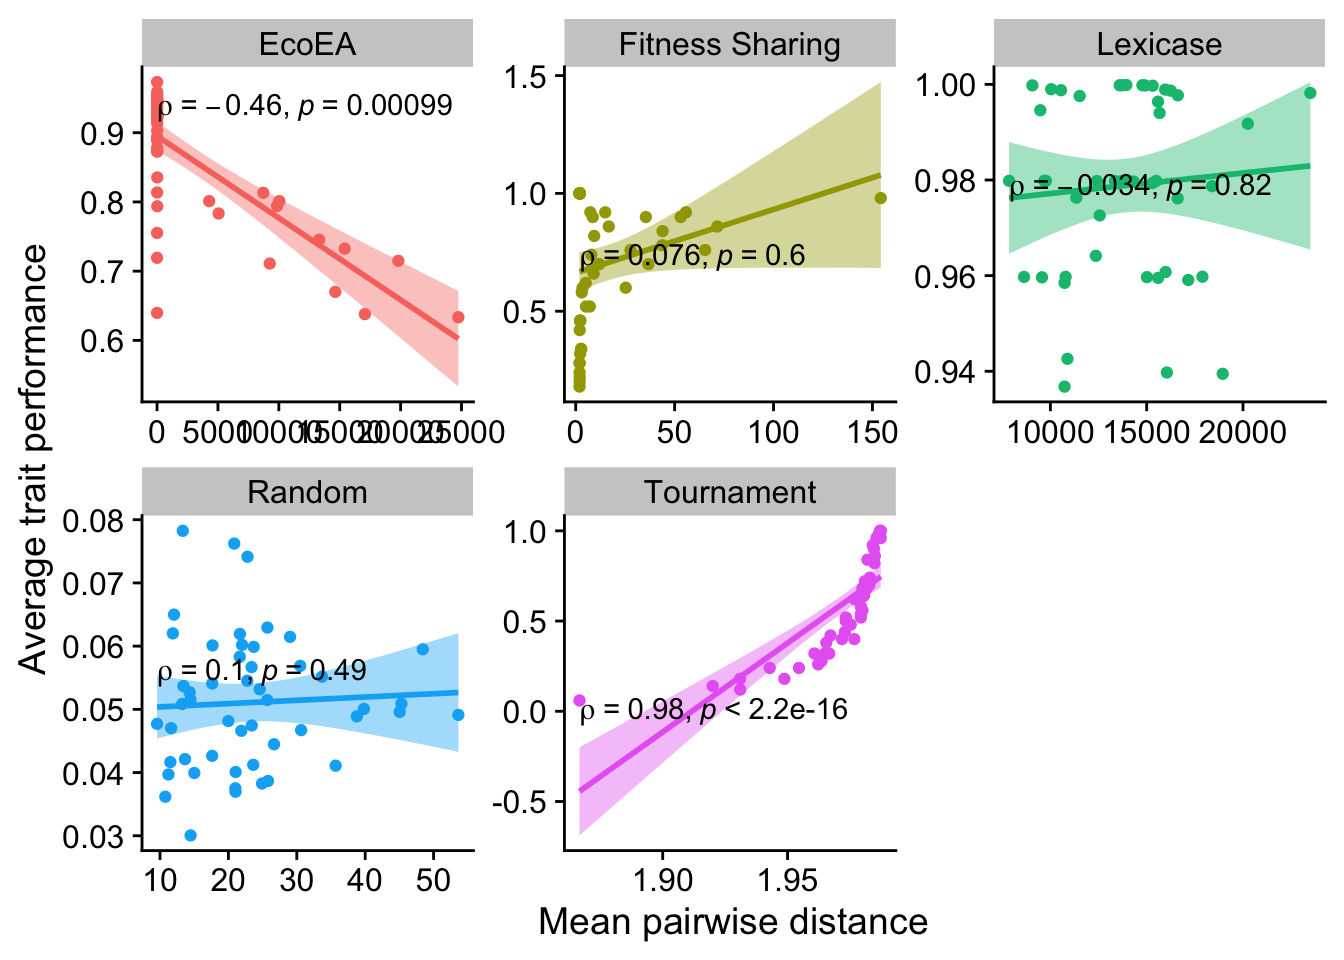
\includegraphics{phylodiversity-in-EC-supplement_files/figure-latex/phylogeny_vs_performance-1.pdf}

\hypertarget{mean-evolutionary-distinctiveness-4}{%
\subsubsection{Mean evolutionary distinctiveness}\label{mean-evolutionary-distinctiveness-4}}

\begin{Shaded}
\begin{Highlighting}[]
\KeywordTok{ggplot}\NormalTok{(}
\NormalTok{    final_data,}
    \KeywordTok{aes}\NormalTok{(}
        \DataTypeTok{y=}\NormalTok{elite_trait_avg,}
        \DataTypeTok{x=}\NormalTok{mean_phenotype_evolutionary_distinctiveness,}
        \DataTypeTok{color=}\NormalTok{selection_name,}
        \DataTypeTok{fill=}\NormalTok{selection_name}
\NormalTok{    )}
\NormalTok{  ) }\OperatorTok{+}
\StringTok{  }\KeywordTok{geom_point}\NormalTok{() }\OperatorTok{+}
\StringTok{    }\KeywordTok{scale_y_continuous}\NormalTok{(}
        \DataTypeTok{name=}\StringTok{"Average trait performance"}
\NormalTok{  ) }\OperatorTok{+}
\StringTok{  }\KeywordTok{scale_x_continuous}\NormalTok{(}
        \DataTypeTok{name=}\StringTok{"Mean evolutionary distinctiveness"}
\NormalTok{  ) }\OperatorTok{+}\StringTok{ }
\StringTok{  }\KeywordTok{facet_wrap}\NormalTok{(}
      \OperatorTok{~}\NormalTok{selection_name, }\DataTypeTok{scales=}\StringTok{"free"}
\NormalTok{  ) }\OperatorTok{+}\StringTok{ }
\StringTok{  }\KeywordTok{stat_smooth}\NormalTok{(}
    \DataTypeTok{method=}\StringTok{"lm"}
\NormalTok{  ) }\OperatorTok{+}\StringTok{ }
\StringTok{  }\KeywordTok{stat_cor}\NormalTok{(}
    \DataTypeTok{method=}\StringTok{"spearman"}\NormalTok{, }\DataTypeTok{cor.coef.name =} \StringTok{"rho"}\NormalTok{, }\DataTypeTok{color=}\StringTok{"black"}
\NormalTok{  ) }\OperatorTok{+}
\StringTok{  }\KeywordTok{theme}\NormalTok{(}\DataTypeTok{legend.position =} \StringTok{"none"}\NormalTok{)}
\end{Highlighting}
\end{Shaded}

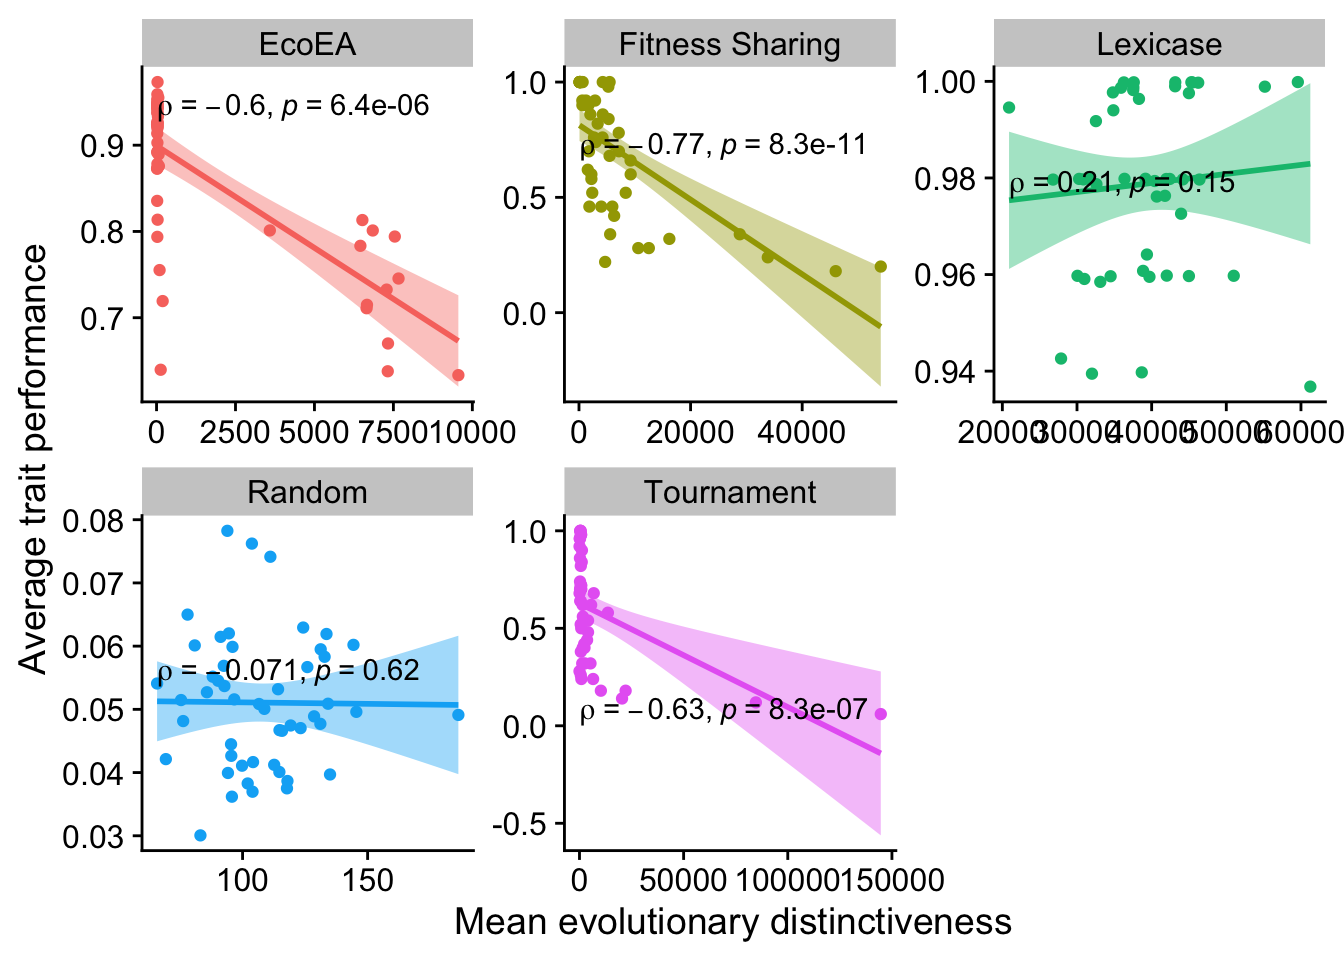
\includegraphics{phylodiversity-in-EC-supplement_files/figure-latex/med_vs_performance-1.pdf}

\hypertarget{richness-4}{%
\subsubsection{Richness}\label{richness-4}}

\begin{Shaded}
\begin{Highlighting}[]
\KeywordTok{ggplot}\NormalTok{(}
\NormalTok{    final_data,}
    \KeywordTok{aes}\NormalTok{(}
        \DataTypeTok{y=}\NormalTok{elite_trait_avg,}
        \DataTypeTok{x=}\NormalTok{phen_num_taxa,}
        \DataTypeTok{color=}\NormalTok{selection_name,}
        \DataTypeTok{fill=}\NormalTok{selection_name}
\NormalTok{    )}
\NormalTok{  ) }\OperatorTok{+}
\StringTok{  }\KeywordTok{geom_point}\NormalTok{() }\OperatorTok{+}
\StringTok{    }\KeywordTok{scale_y_continuous}\NormalTok{(}
        \DataTypeTok{name=}\StringTok{"Average trait performance"}
\NormalTok{  ) }\OperatorTok{+}
\StringTok{  }\KeywordTok{scale_x_continuous}\NormalTok{(}
        \DataTypeTok{name=}\StringTok{"Phenotypic richness"}
\NormalTok{  ) }\OperatorTok{+}\StringTok{ }
\StringTok{  }\KeywordTok{facet_wrap}\NormalTok{(}
      \OperatorTok{~}\NormalTok{selection_name, }\DataTypeTok{scales=}\StringTok{"free"}
\NormalTok{  ) }\OperatorTok{+}\StringTok{ }
\StringTok{  }\KeywordTok{stat_smooth}\NormalTok{(}
    \DataTypeTok{method=}\StringTok{"lm"}
\NormalTok{  ) }\OperatorTok{+}\StringTok{ }
\StringTok{  }\KeywordTok{stat_cor}\NormalTok{(}
    \DataTypeTok{method=}\StringTok{"spearman"}\NormalTok{, }\DataTypeTok{cor.coef.name =} \StringTok{"rho"}\NormalTok{, }\DataTypeTok{color=}\StringTok{"black"}
\NormalTok{  ) }\OperatorTok{+}
\StringTok{  }\KeywordTok{theme}\NormalTok{(}\DataTypeTok{legend.position =} \StringTok{"none"}\NormalTok{)}
\end{Highlighting}
\end{Shaded}

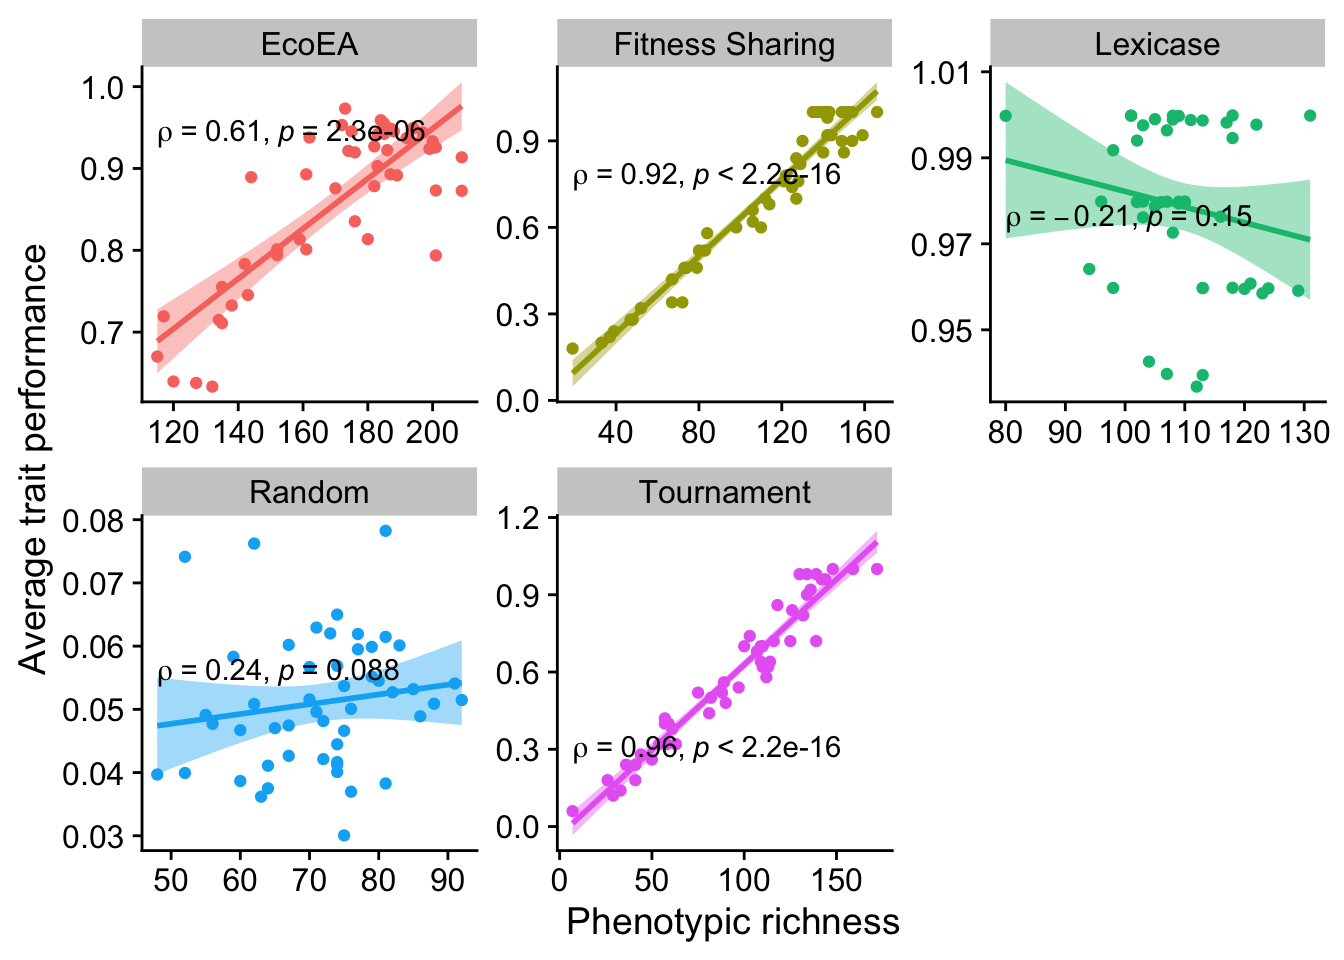
\includegraphics{phylodiversity-in-EC-supplement_files/figure-latex/richness_vs_performance-1.pdf}

\hypertarget{shannon-diversity-4}{%
\subsubsection{Shannon diversity}\label{shannon-diversity-4}}

\begin{Shaded}
\begin{Highlighting}[]
\KeywordTok{ggplot}\NormalTok{(}
\NormalTok{    final_data,}
    \KeywordTok{aes}\NormalTok{(}
        \DataTypeTok{y=}\NormalTok{elite_trait_avg,}
        \DataTypeTok{x=}\NormalTok{phen_diversity,}
        \DataTypeTok{color=}\NormalTok{selection_name,}
        \DataTypeTok{fill=}\NormalTok{selection_name}
\NormalTok{    )}
\NormalTok{  ) }\OperatorTok{+}
\StringTok{  }\KeywordTok{geom_point}\NormalTok{() }\OperatorTok{+}
\StringTok{    }\KeywordTok{scale_y_continuous}\NormalTok{(}
        \DataTypeTok{name=}\StringTok{"Average trait performance"}
\NormalTok{  ) }\OperatorTok{+}
\StringTok{  }\KeywordTok{scale_x_continuous}\NormalTok{(}
        \DataTypeTok{name=}\StringTok{"Phenotypic Shannon diversity"}
\NormalTok{  ) }\OperatorTok{+}\StringTok{ }
\StringTok{  }\KeywordTok{facet_wrap}\NormalTok{(}
      \OperatorTok{~}\NormalTok{selection_name, }\DataTypeTok{scales=}\StringTok{"free"}
\NormalTok{  ) }\OperatorTok{+}\StringTok{ }
\StringTok{  }\KeywordTok{stat_smooth}\NormalTok{(}
    \DataTypeTok{method=}\StringTok{"lm"}
\NormalTok{  ) }\OperatorTok{+}\StringTok{ }
\StringTok{  }\KeywordTok{stat_cor}\NormalTok{(}
    \DataTypeTok{method=}\StringTok{"spearman"}\NormalTok{, }\DataTypeTok{cor.coef.name =} \StringTok{"rho"}\NormalTok{, }\DataTypeTok{color=}\StringTok{"black"}
\NormalTok{  ) }\OperatorTok{+}
\StringTok{  }\KeywordTok{theme}\NormalTok{(}\DataTypeTok{legend.position =} \StringTok{"none"}\NormalTok{)}
\end{Highlighting}
\end{Shaded}

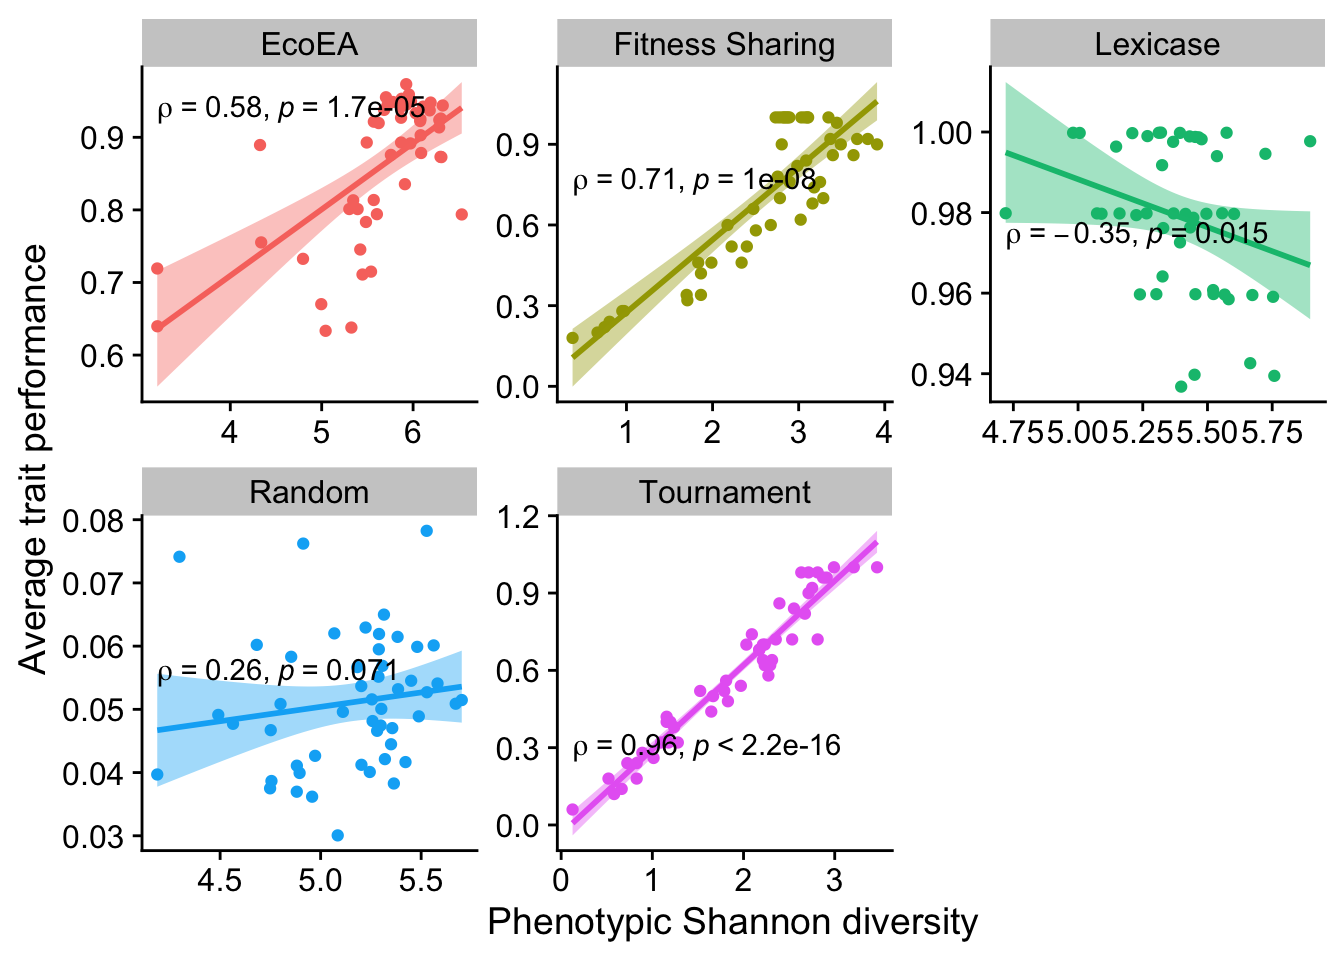
\includegraphics{phylodiversity-in-EC-supplement_files/figure-latex/shannon_vs_performance-1.pdf}

\hypertarget{causality-analysis}{%
\section{Causality analysis}\label{causality-analysis}}

Ultimately, it's hard to draw useful inferences either from these single time point analyses or from comparison of line plots. Due to the feedbacks between diversity and performance, there may be a time delay in when one affects the other.

To analyze the drivers of this feedback loop in a more rigorous way, we turn to \href{https://towardsdatascience.com/causality-931372313a1c}{Transfer Entropy} as a metric of \href{http://www.scholarpedia.org/article/Granger_causality}{Granger Causality}. For a more thorough description, see the paper associated with this supplement.

\hypertarget{setup-1}{%
\subsection{Setup}\label{setup-1}}

First let's define a function we'll use to calculate and output significance and effect size for these results:

\begin{Shaded}
\begin{Highlighting}[]
\NormalTok{transfer_entropy_stats <-}\StringTok{ }\ControlFlowTok{function}\NormalTok{(res) \{}
\NormalTok{  stat.test <-}\StringTok{ }\NormalTok{res }\OperatorTok
\StringTok{    }\KeywordTok{group_by}\NormalTok{(selection_name, offset) }\OperatorTok
\StringTok{    }\KeywordTok{wilcox_test}\NormalTok{(value }\OperatorTok{~}\StringTok{ }\NormalTok{Type) }\OperatorTok
\StringTok{    }\KeywordTok{adjust_pvalue}\NormalTok{(}\DataTypeTok{method =} \StringTok{"bonferroni"}\NormalTok{) }\OperatorTok
\StringTok{    }\KeywordTok{add_significance}\NormalTok{() }
\NormalTok{  stat.test}\OperatorTok{$}\NormalTok{label <-}\StringTok{ }\KeywordTok{mapply}\NormalTok{(p_label,stat.test}\OperatorTok{$}\NormalTok{p.adj)}
  
  \CommentTok{# Calculate effect sizes for these differences}
\NormalTok{  effect_sizes <-}\StringTok{ }\NormalTok{res }\OperatorTok
\StringTok{    }\KeywordTok{group_by}\NormalTok{(selection_name, offset) }\OperatorTok
\StringTok{    }\KeywordTok{wilcox_effsize}\NormalTok{(value }\OperatorTok{~}\StringTok{ }\NormalTok{Type)}
  
\NormalTok{  stat.test}\OperatorTok{$}\NormalTok{effsize <-}\StringTok{ }\NormalTok{effect_sizes}\OperatorTok{$}\NormalTok{effsize}
\NormalTok{  stat.test}\OperatorTok{$}\NormalTok{magnitude <-}\StringTok{ }\NormalTok{effect_sizes}\OperatorTok{$}\NormalTok{magnitude}
  
\NormalTok{  stat.test }\OperatorTok
\StringTok{    }\KeywordTok{kbl}\NormalTok{() }\OperatorTok
\StringTok{    }\KeywordTok{kable_styling}\NormalTok{(}
      \DataTypeTok{bootstrap_options =} \KeywordTok{c}\NormalTok{(}
        \StringTok{"striped"}\NormalTok{,}
        \StringTok{"hover"}\NormalTok{,}
        \StringTok{"condensed"}\NormalTok{,}
        \StringTok{"responsive"}
\NormalTok{      )}
\NormalTok{    ) }\OperatorTok
\StringTok{    }\KeywordTok{scroll_box}\NormalTok{()}
\NormalTok{\}}
\end{Highlighting}
\end{Shaded}

\hypertarget{transfer-entropy-from-diversity-to-fitness}{%
\subsection{Transfer entropy from diversity to fitness}\label{transfer-entropy-from-diversity-to-fitness}}

First, we calculate the information that each type of diversity gives us about future fitness.

\hypertarget{max-pairwise-distance-vs.phenotypic-richness}{%
\subsubsection{Max pairwise distance vs.~phenotypic richness}\label{max-pairwise-distance-vs.phenotypic-richness}}

We plot the differences in transfer entropy from phylogenetic diversity to fitness and from phenotypic diversity to fitness, at a range of different lags.

\begin{Shaded}
\begin{Highlighting}[]
\CommentTok{# Calculate transfer entropy for max pairwise distance}
\CommentTok{# Time points are 10 generations, so calculating lag 1 gives us lag 10}
\NormalTok{res <-}\StringTok{ }\NormalTok{data }\OperatorTok\StringTok{ }\KeywordTok{group_by}\NormalTok{(directory, selection_name) }\OperatorTok
\KeywordTok{summarise}\NormalTok{(}
  \DataTypeTok{fit_phylo_10 =}     \KeywordTok{condinformation}\NormalTok{(}\KeywordTok{discretize}\NormalTok{(elite_trait_avg), }\CommentTok{# TE phylo -> fit, lag 10}
                                     \KeywordTok{discretize}\NormalTok{(}\KeywordTok{lag}\NormalTok{(max_phenotype_pairwise_distance, }\DecValTok{1}\NormalTok{)), }
                                     \KeywordTok{discretize}\NormalTok{(}\KeywordTok{lag}\NormalTok{(elite_trait_avg, }\DecValTok{1}\NormalTok{))),}
  \DataTypeTok{fit_phylo_100 =}    \KeywordTok{condinformation}\NormalTok{(}\KeywordTok{discretize}\NormalTok{(elite_trait_avg), }\CommentTok{# TE phylo -> fit, lag 100}
                                     \KeywordTok{discretize}\NormalTok{(}\KeywordTok{lag}\NormalTok{(max_phenotype_pairwise_distance, }\DecValTok{10}\NormalTok{)), }
                                     \KeywordTok{discretize}\NormalTok{(}\KeywordTok{lag}\NormalTok{(elite_trait_avg, }\DecValTok{10}\NormalTok{))),}
  \DataTypeTok{fit_phylo_1000 =}   \KeywordTok{condinformation}\NormalTok{(}\KeywordTok{discretize}\NormalTok{(elite_trait_avg), }\CommentTok{# TE phylo -> fit, lag 1000}
                                     \KeywordTok{discretize}\NormalTok{(}\KeywordTok{lag}\NormalTok{(max_phenotype_pairwise_distance, }\DecValTok{100}\NormalTok{)), }
                                     \KeywordTok{discretize}\NormalTok{(}\KeywordTok{lag}\NormalTok{(elite_trait_avg, }\DecValTok{100}\NormalTok{))),}
  \DataTypeTok{fit_phylo_10000 =}  \KeywordTok{condinformation}\NormalTok{(}\KeywordTok{discretize}\NormalTok{(elite_trait_avg), }\CommentTok{# TE phylo -> fit, lag 10000}
                                     \KeywordTok{discretize}\NormalTok{(}\KeywordTok{lag}\NormalTok{(max_phenotype_pairwise_distance, }\DecValTok{1000}\NormalTok{)), }
                                     \KeywordTok{discretize}\NormalTok{(}\KeywordTok{lag}\NormalTok{(elite_trait_avg, }\DecValTok{1000}\NormalTok{))),}
  \DataTypeTok{fit_phylo_100000 =} \KeywordTok{condinformation}\NormalTok{(}\KeywordTok{discretize}\NormalTok{(elite_trait_avg), }\CommentTok{# TE phylo -> fit, lag 100000}
                                     \KeywordTok{discretize}\NormalTok{(}\KeywordTok{lag}\NormalTok{(max_phenotype_pairwise_distance, }\DecValTok{10000}\NormalTok{)), }
                                     \KeywordTok{discretize}\NormalTok{(}\KeywordTok{lag}\NormalTok{(elite_trait_avg, }\DecValTok{10000}\NormalTok{))),  }
  \DataTypeTok{fit_fit_10000 =}    \KeywordTok{condinformation}\NormalTok{(}\KeywordTok{discretize}\NormalTok{(elite_trait_avg), }\CommentTok{# Mutual info btwn. fit and lagged fit}
                                     \KeywordTok{discretize}\NormalTok{(}\KeywordTok{lag}\NormalTok{(elite_trait_avg, }\DecValTok{1000}\NormalTok{)), }
                                     \KeywordTok{discretize}\NormalTok{(}\KeywordTok{lag}\NormalTok{(max_phenotype_pairwise_distance, }\DecValTok{1000}\NormalTok{))),}
  \DataTypeTok{fit_fit_100000 =}   \KeywordTok{condinformation}\NormalTok{(}\KeywordTok{discretize}\NormalTok{(elite_trait_avg), }\CommentTok{# Mutual info btwn. fit and lagged fit}
                                     \KeywordTok{discretize}\NormalTok{(}\KeywordTok{lag}\NormalTok{(elite_trait_avg, }\DecValTok{10000}\NormalTok{)), }
                                     \KeywordTok{discretize}\NormalTok{(}\KeywordTok{lag}\NormalTok{(max_phenotype_pairwise_distance, }\DecValTok{10000}\NormalTok{))),  }
  \DataTypeTok{fit_pheno_10 =}     \KeywordTok{condinformation}\NormalTok{(}\KeywordTok{discretize}\NormalTok{(elite_trait_avg), }\CommentTok{# TE pheno -> fit, lag 10}
                                     \KeywordTok{discretize}\NormalTok{(}\KeywordTok{lag}\NormalTok{(phen_num_taxa, }\DecValTok{1}\NormalTok{)), }
                                     \KeywordTok{discretize}\NormalTok{(}\KeywordTok{lag}\NormalTok{(elite_trait_avg, }\DecValTok{1}\NormalTok{))),}
  \DataTypeTok{fit_pheno_100 =}    \KeywordTok{condinformation}\NormalTok{(}\KeywordTok{discretize}\NormalTok{(elite_trait_avg),  }\CommentTok{# TE pheno -> fit, lag 100 }
                                     \KeywordTok{discretize}\NormalTok{(}\KeywordTok{lag}\NormalTok{(phen_num_taxa, }\DecValTok{10}\NormalTok{)), }
                                     \KeywordTok{discretize}\NormalTok{(}\KeywordTok{lag}\NormalTok{(elite_trait_avg, }\DecValTok{10}\NormalTok{))),}
  \DataTypeTok{fit_pheno_1000 =}   \KeywordTok{condinformation}\NormalTok{(}\KeywordTok{discretize}\NormalTok{(elite_trait_avg),  }\CommentTok{# TE pheno -> fit, lag 1000}
                                     \KeywordTok{discretize}\NormalTok{(}\KeywordTok{lag}\NormalTok{(phen_num_taxa, }\DecValTok{100}\NormalTok{)), }
                                     \KeywordTok{discretize}\NormalTok{(}\KeywordTok{lag}\NormalTok{(elite_trait_avg, }\DecValTok{100}\NormalTok{))),}
  \DataTypeTok{fit_pheno_10000 =}  \KeywordTok{condinformation}\NormalTok{(}\KeywordTok{discretize}\NormalTok{(elite_trait_avg),  }\CommentTok{# TE pheno -> fit, lag 10000}
                                     \KeywordTok{discretize}\NormalTok{(}\KeywordTok{lag}\NormalTok{(phen_num_taxa, }\DecValTok{1000}\NormalTok{)), }
                                     \KeywordTok{discretize}\NormalTok{(}\KeywordTok{lag}\NormalTok{(elite_trait_avg, }\DecValTok{1000}\NormalTok{))),}
  \DataTypeTok{fit_pheno_100000 =} \KeywordTok{condinformation}\NormalTok{(}\KeywordTok{discretize}\NormalTok{(elite_trait_avg),  }\CommentTok{# TE pheno -> fit, lag 100000}
                                     \KeywordTok{discretize}\NormalTok{(}\KeywordTok{lag}\NormalTok{(phen_num_taxa, }\DecValTok{10000}\NormalTok{)), }
                                     \KeywordTok{discretize}\NormalTok{(}\KeywordTok{lag}\NormalTok{(elite_trait_avg, }\DecValTok{10000}\NormalTok{)))}
\NormalTok{)}

\CommentTok{# Turn Transfer Entropy columns into rows}
\NormalTok{res <-}\StringTok{ }\NormalTok{res }\OperatorTok\StringTok{ }\KeywordTok{pivot_longer}\NormalTok{(}\DataTypeTok{cols=}\KeywordTok{contains}\NormalTok{(}\StringTok{"o_10"}\NormalTok{))}
\CommentTok{# Pull lag into a column}
\NormalTok{res}\OperatorTok{$}\NormalTok{offset <-}\StringTok{ }\KeywordTok{str_extract}\NormalTok{(res}\OperatorTok{$}\NormalTok{name, }\StringTok{"[:digit:]*$"}\NormalTok{)}
\CommentTok{# Make column indicating direction of transfer entropy}
\NormalTok{res}\OperatorTok{$}\NormalTok{Type <-}\StringTok{ }\KeywordTok{case_when}\NormalTok{(}\KeywordTok{str_detect}\NormalTok{(res}\OperatorTok{$}\NormalTok{name, }\StringTok{"phylo"}\NormalTok{) }\OperatorTok{~}\StringTok{ "Phylogenetic"}\NormalTok{, }\OtherTok{TRUE} \OperatorTok{~}\StringTok{ "Phenotypic"}\NormalTok{)}

\CommentTok{# Plot transfer entropy}
\KeywordTok{ggplot}\NormalTok{(}
\NormalTok{  res }\OperatorTok\StringTok{ }\KeywordTok{filter}\NormalTok{(}\KeywordTok{str_detect}\NormalTok{(name, }\StringTok{"fit_ph*"}\NormalTok{)), }
  \KeywordTok{aes}\NormalTok{(}
    \DataTypeTok{x=}\KeywordTok{as.factor}\NormalTok{(offset), }
    \DataTypeTok{y=}\NormalTok{value, }
    \DataTypeTok{color=}\NormalTok{Type}
\NormalTok{    )}
\NormalTok{  ) }\OperatorTok{+}\StringTok{ }
\StringTok{  }\KeywordTok{geom_boxplot}\NormalTok{() }\OperatorTok{+}\StringTok{ }
\StringTok{  }\KeywordTok{facet_wrap}\NormalTok{(}\OperatorTok{~}\NormalTok{selection_name) }\OperatorTok{+}\StringTok{ }
\StringTok{  }\KeywordTok{scale_x_discrete}\NormalTok{(}\StringTok{"Lag"}\NormalTok{,}\DataTypeTok{labels=}\KeywordTok{c}\NormalTok{(}\StringTok{"10"}\NormalTok{,}\StringTok{""}\NormalTok{,}\StringTok{"1000"}\NormalTok{,}\StringTok{""}\NormalTok{,}\StringTok{"100000"}\NormalTok{)) }\OperatorTok{+}\StringTok{ }
\StringTok{  }\KeywordTok{scale_y_continuous}\NormalTok{(}\StringTok{"Transfer Entropy"}\NormalTok{) }\OperatorTok{+}\StringTok{ }
\StringTok{  }\KeywordTok{theme}\NormalTok{(}\DataTypeTok{legend.position =} \KeywordTok{c}\NormalTok{(}\DecValTok{1}\NormalTok{, }\DecValTok{0}\NormalTok{),}
        \DataTypeTok{legend.justification =} \KeywordTok{c}\NormalTok{(}\DecValTok{1}\NormalTok{, }\DecValTok{0}\NormalTok{)) }\OperatorTok{+}\StringTok{ }
\StringTok{  }\KeywordTok{scale_color_discrete}\NormalTok{(}\StringTok{""}\NormalTok{)}
\end{Highlighting}
\end{Shaded}

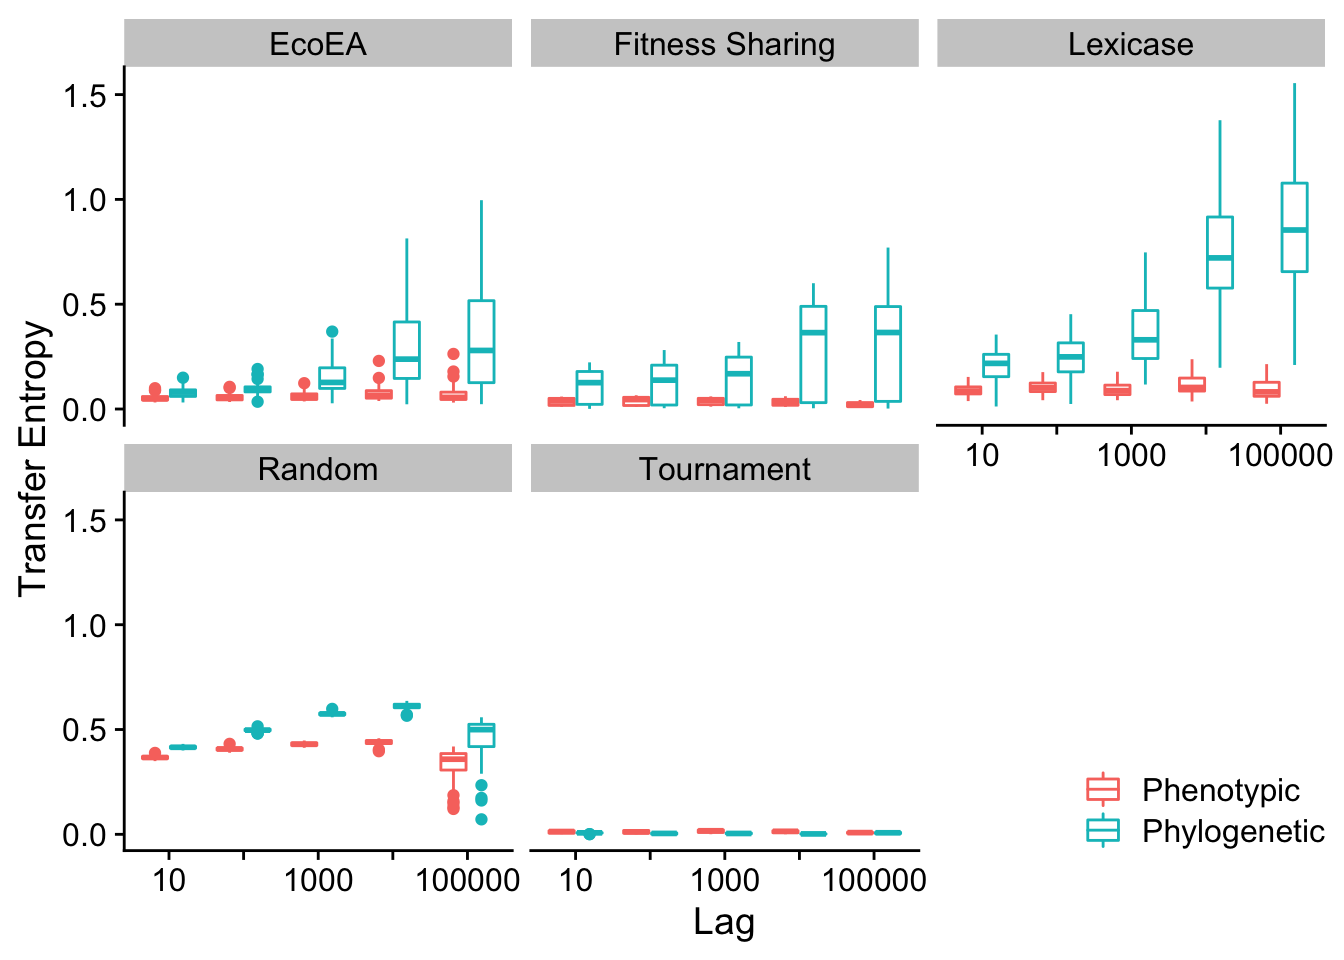
\includegraphics{phylodiversity-in-EC-supplement_files/figure-latex/information_theory-1.pdf}

Next we calculate statistics to quantify these differences

\begin{Shaded}
\begin{Highlighting}[]
\CommentTok{# Determine which conditions are significantly different from each other}
\KeywordTok{transfer_entropy_stats}\NormalTok{(res)}
\end{Highlighting}
\end{Shaded}

\begin{table}
\centering
\begin{tabular}[t]{l|l|l|l|l|r|r|r|r|r|l|l|r|l}
\hline
selection\_name & offset & .y. & group1 & group2 & n1 & n2 & statistic & p & p.adj & p.adj.signif & label & effsize & magnitude\\
\hline
EcoEA & 10 & value & Phenotypic & Phylogenetic & 50 & 50 & 463 & 1.00e-07 & 0.0000015 & **** & p < 1e-04 & 0.5425436 & large\\
\hline
EcoEA & 100 & value & Phenotypic & Phylogenetic & 50 & 50 & 242 & 0.00e+00 & 0.0000000 & **** & p < 1e-04 & 0.6948970 & large\\
\hline
EcoEA & 1000 & value & Phenotypic & Phylogenetic & 50 & 50 & 195 & 0.00e+00 & 0.0000000 & **** & p < 1e-04 & 0.7272980 & large\\
\hline
EcoEA & 10000 & value & Phenotypic & Phylogenetic & 50 & 50 & 163 & 0.00e+00 & 0.0000000 & **** & p < 1e-04 & 0.7493582 & large\\
\hline
EcoEA & 100000 & value & Phenotypic & Phylogenetic & 50 & 50 & 247 & 0.00e+00 & 0.0000000 & **** & p < 1e-04 & 0.6914501 & large\\
\hline
Fitness Sharing & 10 & value & Phenotypic & Phylogenetic & 50 & 50 & 699 & 1.48e-04 & 0.0037000 & ** & p = 0.0037 & 0.3798495 & moderate\\
\hline
Fitness Sharing & 100 & value & Phenotypic & Phylogenetic & 50 & 50 & 739 & 4.33e-04 & 0.0108250 & * & p = 0.010825 & 0.3522742 & moderate\\
\hline
Fitness Sharing & 1000 & value & Phenotypic & Phylogenetic & 50 & 50 & 751 & 5.89e-04 & 0.0147250 & * & p = 0.014725 & 0.3440016 & moderate\\
\hline
Fitness Sharing & 10000 & value & Phenotypic & Phylogenetic & 50 & 50 & 598 & 7.10e-06 & 0.0001770 & *** & p = 0.000177 & 0.4494771 & moderate\\
\hline
Fitness Sharing & 100000 & value & Phenotypic & Phylogenetic & 50 & 50 & 415 & 0.00e+00 & 0.0000002 & **** & p < 1e-04 & 0.5756340 & large\\
\hline
Lexicase & 10 & value & Phenotypic & Phylogenetic & 50 & 50 & 194 & 0.00e+00 & 0.0000000 & **** & p < 1e-04 & 0.7279874 & large\\
\hline
Lexicase & 100 & value & Phenotypic & Phylogenetic & 50 & 50 & 183 & 0.00e+00 & 0.0000000 & **** & p < 1e-04 & 0.7355706 & large\\
\hline
Lexicase & 1000 & value & Phenotypic & Phylogenetic & 50 & 50 & 36 & 0.00e+00 & 0.0000000 & **** & p < 1e-04 & 0.8369097 & large\\
\hline
Lexicase & 10000 & value & Phenotypic & Phylogenetic & 50 & 50 & 1 & 0.00e+00 & 0.0000000 & **** & p < 1e-04 & 0.8610381 & large\\
\hline
Lexicase & 100000 & value & Phenotypic & Phylogenetic & 50 & 50 & 0 & 0.00e+00 & 0.0000000 & **** & p < 1e-04 & 0.8617275 & large\\
\hline
Random & 10 & value & Phenotypic & Phylogenetic & 50 & 50 & 0 & 0.00e+00 & 0.0000000 & **** & p < 1e-04 & 0.8617275 & large\\
\hline
Random & 100 & value & Phenotypic & Phylogenetic & 50 & 50 & 0 & 0.00e+00 & 0.0000000 & **** & p < 1e-04 & 0.8617275 & large\\
\hline
Random & 1000 & value & Phenotypic & Phylogenetic & 50 & 50 & 0 & 0.00e+00 & 0.0000000 & **** & p < 1e-04 & 0.8617275 & large\\
\hline
Random & 10000 & value & Phenotypic & Phylogenetic & 50 & 50 & 0 & 0.00e+00 & 0.0000000 & **** & p < 1e-04 & 0.8617275 & large\\
\hline
Random & 100000 & value & Phenotypic & Phylogenetic & 50 & 50 & 249 & 0.00e+00 & 0.0000000 & **** & p < 1e-04 & 0.6900714 & large\\
\hline
Tournament & 10 & value & Phenotypic & Phylogenetic & 50 & 50 & 1798 & 1.60e-04 & 0.0040000 & ** & p = 0.004 & 0.3777813 & moderate\\
\hline
Tournament & 100 & value & Phenotypic & Phylogenetic & 50 & 50 & 2049 & 0.00e+00 & 0.0000009 & **** & p < 1e-04 & 0.5508162 & large\\
\hline
Tournament & 1000 & value & Phenotypic & Phylogenetic & 50 & 50 & 2232 & 0.00e+00 & 0.0000000 & **** & p < 1e-04 & 0.6769731 & large\\
\hline
Tournament & 10000 & value & Phenotypic & Phylogenetic & 50 & 50 & 2329 & 0.00e+00 & 0.0000000 & **** & p < 1e-04 & 0.7438432 & large\\
\hline
Tournament & 100000 & value & Phenotypic & Phylogenetic & 50 & 50 & 1418 & 2.48e-01 & 1.0000000 & ns & p = 1 & 0.1158162 & small\\
\hline
\end{tabular}
\end{table}

\hypertarget{mean-pairwise-distance-vs.phenotypic-richness}{%
\subsubsection{Mean pairwise distance vs.~phenotypic richness}\label{mean-pairwise-distance-vs.phenotypic-richness}}

\begin{Shaded}
\begin{Highlighting}[]
\CommentTok{# Calculate transfer entropy for mean pairwise distance}
\CommentTok{# Time points are 10 generations, so calculating lag 1 gives us lag 10}
\NormalTok{res <-}\StringTok{ }\NormalTok{data }\OperatorTok\StringTok{ }\KeywordTok{group_by}\NormalTok{(directory, selection_name) }\OperatorTok
\KeywordTok{summarise}\NormalTok{(}
  \DataTypeTok{fit_phylo_10 =}     \KeywordTok{condinformation}\NormalTok{(}\KeywordTok{discretize}\NormalTok{(elite_trait_avg), }\CommentTok{# TE phylo -> fit, lag 10}
                                     \KeywordTok{discretize}\NormalTok{(}\KeywordTok{lag}\NormalTok{(mean_phenotype_pairwise_distance, }\DecValTok{1}\NormalTok{)), }
                                     \KeywordTok{discretize}\NormalTok{(}\KeywordTok{lag}\NormalTok{(elite_trait_avg, }\DecValTok{1}\NormalTok{))),}
  \DataTypeTok{fit_phylo_100 =}    \KeywordTok{condinformation}\NormalTok{(}\KeywordTok{discretize}\NormalTok{(elite_trait_avg), }\CommentTok{# TE phylo -> fit, lag 100}
                                     \KeywordTok{discretize}\NormalTok{(}\KeywordTok{lag}\NormalTok{(mean_phenotype_pairwise_distance, }\DecValTok{10}\NormalTok{)), }
                                     \KeywordTok{discretize}\NormalTok{(}\KeywordTok{lag}\NormalTok{(elite_trait_avg, }\DecValTok{10}\NormalTok{))),}
  \DataTypeTok{fit_phylo_1000 =}   \KeywordTok{condinformation}\NormalTok{(}\KeywordTok{discretize}\NormalTok{(elite_trait_avg), }\CommentTok{# TE phylo -> fit, lag 1000}
                                     \KeywordTok{discretize}\NormalTok{(}\KeywordTok{lag}\NormalTok{(mean_phenotype_pairwise_distance, }\DecValTok{100}\NormalTok{)), }
                                     \KeywordTok{discretize}\NormalTok{(}\KeywordTok{lag}\NormalTok{(elite_trait_avg, }\DecValTok{100}\NormalTok{))),}
  \DataTypeTok{fit_phylo_10000 =}  \KeywordTok{condinformation}\NormalTok{(}\KeywordTok{discretize}\NormalTok{(elite_trait_avg), }\CommentTok{# TE phylo -> fit, lag 10000}
                                     \KeywordTok{discretize}\NormalTok{(}\KeywordTok{lag}\NormalTok{(mean_phenotype_pairwise_distance, }\DecValTok{1000}\NormalTok{)), }
                                     \KeywordTok{discretize}\NormalTok{(}\KeywordTok{lag}\NormalTok{(elite_trait_avg, }\DecValTok{1000}\NormalTok{))),}
  \DataTypeTok{fit_phylo_100000 =} \KeywordTok{condinformation}\NormalTok{(}\KeywordTok{discretize}\NormalTok{(elite_trait_avg), }\CommentTok{# TE phylo -> fit, lag 100000}
                                     \KeywordTok{discretize}\NormalTok{(}\KeywordTok{lag}\NormalTok{(mean_phenotype_pairwise_distance, }\DecValTok{10000}\NormalTok{)), }
                                     \KeywordTok{discretize}\NormalTok{(}\KeywordTok{lag}\NormalTok{(elite_trait_avg, }\DecValTok{10000}\NormalTok{))),  }
  \DataTypeTok{fit_fit_10000 =}    \KeywordTok{condinformation}\NormalTok{(}\KeywordTok{discretize}\NormalTok{(elite_trait_avg), }\CommentTok{# Mutual info btwn. fit and lagged fit}
                                     \KeywordTok{discretize}\NormalTok{(}\KeywordTok{lag}\NormalTok{(elite_trait_avg, }\DecValTok{1000}\NormalTok{)), }
                                     \KeywordTok{discretize}\NormalTok{(}\KeywordTok{lag}\NormalTok{(mean_phenotype_pairwise_distance, }\DecValTok{1000}\NormalTok{))),}
  \DataTypeTok{fit_fit_100000 =}   \KeywordTok{condinformation}\NormalTok{(}\KeywordTok{discretize}\NormalTok{(elite_trait_avg), }\CommentTok{# Mutual info btwn. fit and lagged fit}
                                     \KeywordTok{discretize}\NormalTok{(}\KeywordTok{lag}\NormalTok{(elite_trait_avg, }\DecValTok{10000}\NormalTok{)), }
                                     \KeywordTok{discretize}\NormalTok{(}\KeywordTok{lag}\NormalTok{(mean_phenotype_pairwise_distance, }\DecValTok{10000}\NormalTok{))),  }
  \DataTypeTok{fit_pheno_10 =}     \KeywordTok{condinformation}\NormalTok{(}\KeywordTok{discretize}\NormalTok{(elite_trait_avg), }\CommentTok{# TE pheno -> fit, lag 10}
                                     \KeywordTok{discretize}\NormalTok{(}\KeywordTok{lag}\NormalTok{(phen_num_taxa, }\DecValTok{1}\NormalTok{)), }
                                     \KeywordTok{discretize}\NormalTok{(}\KeywordTok{lag}\NormalTok{(elite_trait_avg, }\DecValTok{1}\NormalTok{))),}
  \DataTypeTok{fit_pheno_100 =}    \KeywordTok{condinformation}\NormalTok{(}\KeywordTok{discretize}\NormalTok{(elite_trait_avg),  }\CommentTok{# TE pheno -> fit, lag 100 }
                                     \KeywordTok{discretize}\NormalTok{(}\KeywordTok{lag}\NormalTok{(phen_num_taxa, }\DecValTok{10}\NormalTok{)), }
                                     \KeywordTok{discretize}\NormalTok{(}\KeywordTok{lag}\NormalTok{(elite_trait_avg, }\DecValTok{10}\NormalTok{))),}
  \DataTypeTok{fit_pheno_1000 =}   \KeywordTok{condinformation}\NormalTok{(}\KeywordTok{discretize}\NormalTok{(elite_trait_avg),  }\CommentTok{# TE pheno -> fit, lag 1000}
                                     \KeywordTok{discretize}\NormalTok{(}\KeywordTok{lag}\NormalTok{(phen_num_taxa, }\DecValTok{100}\NormalTok{)), }
                                     \KeywordTok{discretize}\NormalTok{(}\KeywordTok{lag}\NormalTok{(elite_trait_avg, }\DecValTok{100}\NormalTok{))),}
  \DataTypeTok{fit_pheno_10000 =}  \KeywordTok{condinformation}\NormalTok{(}\KeywordTok{discretize}\NormalTok{(elite_trait_avg),  }\CommentTok{# TE pheno -> fit, lag 10000}
                                     \KeywordTok{discretize}\NormalTok{(}\KeywordTok{lag}\NormalTok{(phen_num_taxa, }\DecValTok{1000}\NormalTok{)), }
                                     \KeywordTok{discretize}\NormalTok{(}\KeywordTok{lag}\NormalTok{(elite_trait_avg, }\DecValTok{1000}\NormalTok{))),}
  \DataTypeTok{fit_pheno_100000 =} \KeywordTok{condinformation}\NormalTok{(}\KeywordTok{discretize}\NormalTok{(elite_trait_avg),  }\CommentTok{# TE pheno -> fit, lag 100000}
                                     \KeywordTok{discretize}\NormalTok{(}\KeywordTok{lag}\NormalTok{(phen_num_taxa, }\DecValTok{10000}\NormalTok{)), }
                                     \KeywordTok{discretize}\NormalTok{(}\KeywordTok{lag}\NormalTok{(elite_trait_avg, }\DecValTok{10000}\NormalTok{)))}
\NormalTok{)}

\CommentTok{# Turn Transfer Entropy columns into rows}
\NormalTok{res <-}\StringTok{ }\NormalTok{res }\OperatorTok\StringTok{ }\KeywordTok{pivot_longer}\NormalTok{(}\DataTypeTok{cols=}\KeywordTok{contains}\NormalTok{(}\StringTok{"o_10"}\NormalTok{))}
\CommentTok{# Pull lag into a column}
\NormalTok{res}\OperatorTok{$}\NormalTok{offset <-}\StringTok{ }\KeywordTok{str_extract}\NormalTok{(res}\OperatorTok{$}\NormalTok{name, }\StringTok{"[:digit:]*$"}\NormalTok{)}
\CommentTok{# Make column indicating direction of transfer entropy}
\NormalTok{res}\OperatorTok{$}\NormalTok{Type <-}\StringTok{ }\KeywordTok{case_when}\NormalTok{(}\KeywordTok{str_detect}\NormalTok{(res}\OperatorTok{$}\NormalTok{name, }\StringTok{"phylo"}\NormalTok{) }\OperatorTok{~}\StringTok{ "Phylogenetic"}\NormalTok{, }\OtherTok{TRUE} \OperatorTok{~}\StringTok{ "Phenotypic"}\NormalTok{)}

\CommentTok{# Plot transfer entropy}
\KeywordTok{ggplot}\NormalTok{(}
\NormalTok{  res }\OperatorTok\StringTok{ }\KeywordTok{filter}\NormalTok{(}\KeywordTok{str_detect}\NormalTok{(name, }\StringTok{"fit_ph*"}\NormalTok{)), }
  \KeywordTok{aes}\NormalTok{(}
    \DataTypeTok{x=}\KeywordTok{as.factor}\NormalTok{(offset), }
    \DataTypeTok{y=}\NormalTok{value, }
    \DataTypeTok{color=}\NormalTok{Type}
\NormalTok{    )}
\NormalTok{  ) }\OperatorTok{+}\StringTok{ }
\StringTok{  }\KeywordTok{geom_boxplot}\NormalTok{() }\OperatorTok{+}\StringTok{ }
\StringTok{  }\KeywordTok{facet_wrap}\NormalTok{(}\OperatorTok{~}\NormalTok{selection_name) }\OperatorTok{+}\StringTok{ }
\StringTok{  }\KeywordTok{scale_x_discrete}\NormalTok{(}\StringTok{"Lag"}\NormalTok{,}\DataTypeTok{labels=}\KeywordTok{c}\NormalTok{(}\StringTok{"10"}\NormalTok{,}\StringTok{""}\NormalTok{,}\StringTok{"1000"}\NormalTok{,}\StringTok{""}\NormalTok{,}\StringTok{"100000"}\NormalTok{)) }\OperatorTok{+}\StringTok{ }
\StringTok{  }\KeywordTok{scale_y_continuous}\NormalTok{(}\StringTok{"Transfer Entropy"}\NormalTok{) }\OperatorTok{+}\StringTok{ }
\StringTok{  }\KeywordTok{theme}\NormalTok{(}\DataTypeTok{legend.position =} \KeywordTok{c}\NormalTok{(}\DecValTok{1}\NormalTok{, }\DecValTok{0}\NormalTok{),}
        \DataTypeTok{legend.justification =} \KeywordTok{c}\NormalTok{(}\DecValTok{1}\NormalTok{, }\DecValTok{0}\NormalTok{)) }\OperatorTok{+}\StringTok{ }
\StringTok{  }\KeywordTok{scale_color_discrete}\NormalTok{(}\StringTok{""}\NormalTok{)}
\end{Highlighting}
\end{Shaded}

\includegraphics{phylodiversity-in-EC-supplement_files/figure-latex/information_theory_mpd-1.pdf}

Mean and max pairwise distance appear to behave virtually identically.

\begin{Shaded}
\begin{Highlighting}[]
\CommentTok{# Determine which conditions are significantly different from each other}
\KeywordTok{transfer_entropy_stats}\NormalTok{(res)}
\end{Highlighting}
\end{Shaded}

\begin{table}
\centering
\begin{tabular}[t]{l|l|l|l|l|r|r|r|r|r|l|l|r|l}
\hline
selection\_name & offset & .y. & group1 & group2 & n1 & n2 & statistic & p & p.adj & p.adj.signif & label & effsize & magnitude\\
\hline
EcoEA & 10 & value & Phenotypic & Phylogenetic & 50 & 50 & 292 & 0.00e+00 & 0.0000000 & **** & p < 1e-04 & 0.6604279 & large\\
\hline
EcoEA & 100 & value & Phenotypic & Phylogenetic & 50 & 50 & 251 & 0.00e+00 & 0.0000000 & **** & p < 1e-04 & 0.6886926 & large\\
\hline
EcoEA & 1000 & value & Phenotypic & Phylogenetic & 50 & 50 & 318 & 0.00e+00 & 0.0000000 & **** & p < 1e-04 & 0.6425040 & large\\
\hline
EcoEA & 10000 & value & Phenotypic & Phylogenetic & 50 & 50 & 211 & 0.00e+00 & 0.0000000 & **** & p < 1e-04 & 0.7162679 & large\\
\hline
EcoEA & 100000 & value & Phenotypic & Phylogenetic & 50 & 50 & 374 & 0.00e+00 & 0.0000000 & **** & p < 1e-04 & 0.6038986 & large\\
\hline
Fitness Sharing & 10 & value & Phenotypic & Phylogenetic & 50 & 50 & 522 & 5.00e-07 & 0.0000132 & **** & p < 1e-04 & 0.5018701 & large\\
\hline
Fitness Sharing & 100 & value & Phenotypic & Phylogenetic & 50 & 50 & 550 & 1.40e-06 & 0.0000355 & **** & p < 1e-04 & 0.4825674 & moderate\\
\hline
Fitness Sharing & 1000 & value & Phenotypic & Phylogenetic & 50 & 50 & 620 & 1.43e-05 & 0.0003575 & *** & p = 0.0003575 & 0.4343107 & moderate\\
\hline
Fitness Sharing & 10000 & value & Phenotypic & Phylogenetic & 50 & 50 & 464 & 1.00e-07 & 0.0000015 & **** & p < 1e-04 & 0.5418542 & large\\
\hline
Fitness Sharing & 100000 & value & Phenotypic & Phylogenetic & 50 & 50 & 345 & 0.00e+00 & 0.0000000 & **** & p < 1e-04 & 0.6238907 & large\\
\hline
Lexicase & 10 & value & Phenotypic & Phylogenetic & 50 & 50 & 193 & 0.00e+00 & 0.0000000 & **** & p < 1e-04 & 0.7286768 & large\\
\hline
Lexicase & 100 & value & Phenotypic & Phylogenetic & 50 & 50 & 222 & 0.00e+00 & 0.0000000 & **** & p < 1e-04 & 0.7086847 & large\\
\hline
Lexicase & 1000 & value & Phenotypic & Phylogenetic & 50 & 50 & 336 & 0.00e+00 & 0.0000000 & **** & p < 1e-04 & 0.6300951 & large\\
\hline
Lexicase & 10000 & value & Phenotypic & Phylogenetic & 50 & 50 & 137 & 0.00e+00 & 0.0000000 & **** & p < 1e-04 & 0.7672822 & large\\
\hline
Lexicase & 100000 & value & Phenotypic & Phylogenetic & 50 & 50 & 140 & 0.00e+00 & 0.0000000 & **** & p < 1e-04 & 0.7652140 & large\\
\hline
Random & 10 & value & Phenotypic & Phylogenetic & 50 & 50 & 0 & 0.00e+00 & 0.0000000 & **** & p < 1e-04 & 0.8617275 & large\\
\hline
Random & 100 & value & Phenotypic & Phylogenetic & 50 & 50 & 0 & 0.00e+00 & 0.0000000 & **** & p < 1e-04 & 0.8617275 & large\\
\hline
Random & 1000 & value & Phenotypic & Phylogenetic & 50 & 50 & 0 & 0.00e+00 & 0.0000000 & **** & p < 1e-04 & 0.8617275 & large\\
\hline
Random & 10000 & value & Phenotypic & Phylogenetic & 50 & 50 & 0 & 0.00e+00 & 0.0000000 & **** & p < 1e-04 & 0.8617275 & large\\
\hline
Random & 100000 & value & Phenotypic & Phylogenetic & 50 & 50 & 504 & 3.00e-07 & 0.0000069 & **** & p < 1e-04 & 0.5142790 & large\\
\hline
Tournament & 10 & value & Phenotypic & Phylogenetic & 50 & 50 & 932 & 2.86e-02 & 0.7150000 & ns & p = 0.715 & 0.2192235 & small\\
\hline
Tournament & 100 & value & Phenotypic & Phylogenetic & 50 & 50 & 1106 & 3.23e-01 & 1.0000000 & ns & p = 1 & 0.0992710 & small\\
\hline
Tournament & 1000 & value & Phenotypic & Phylogenetic & 50 & 50 & 1209 & 7.80e-01 & 1.0000000 & ns & p = 1 & 0.0282647 & small\\
\hline
Tournament & 10000 & value & Phenotypic & Phylogenetic & 50 & 50 & 1184 & 6.52e-01 & 1.0000000 & ns & p = 1 & 0.0454992 & small\\
\hline
Tournament & 100000 & value & Phenotypic & Phylogenetic & 50 & 50 & 612 & 1.11e-05 & 0.0002775 & *** & p = 0.0002775 & 0.4398257 & moderate\\
\hline
\end{tabular}
\end{table}

\hypertarget{mean-pairwise-distance-vs.shannon-entropy}{%
\subsubsection{Mean pairwise distance vs.~shannon entropy}\label{mean-pairwise-distance-vs.shannon-entropy}}

\begin{Shaded}
\begin{Highlighting}[]
\CommentTok{# Calculate transfer entropy for mean pairwise distance}
\CommentTok{# Time points are 10 generations, so calculating lag 1 gives us lag 10}
\NormalTok{res <-}\StringTok{ }\NormalTok{data }\OperatorTok\StringTok{ }\KeywordTok{group_by}\NormalTok{(directory, selection_name) }\OperatorTok
\KeywordTok{summarise}\NormalTok{(}
  \DataTypeTok{fit_phylo_10 =}     \KeywordTok{condinformation}\NormalTok{(}\KeywordTok{discretize}\NormalTok{(elite_trait_avg), }\CommentTok{# TE phylo -> fit, lag 10}
                                     \KeywordTok{discretize}\NormalTok{(}\KeywordTok{lag}\NormalTok{(mean_phenotype_pairwise_distance, }\DecValTok{1}\NormalTok{)), }
                                     \KeywordTok{discretize}\NormalTok{(}\KeywordTok{lag}\NormalTok{(elite_trait_avg, }\DecValTok{1}\NormalTok{))),}
  \DataTypeTok{fit_phylo_100 =}    \KeywordTok{condinformation}\NormalTok{(}\KeywordTok{discretize}\NormalTok{(elite_trait_avg), }\CommentTok{# TE phylo -> fit, lag 100}
                                     \KeywordTok{discretize}\NormalTok{(}\KeywordTok{lag}\NormalTok{(mean_phenotype_pairwise_distance, }\DecValTok{10}\NormalTok{)), }
                                     \KeywordTok{discretize}\NormalTok{(}\KeywordTok{lag}\NormalTok{(elite_trait_avg, }\DecValTok{10}\NormalTok{))),}
  \DataTypeTok{fit_phylo_1000 =}   \KeywordTok{condinformation}\NormalTok{(}\KeywordTok{discretize}\NormalTok{(elite_trait_avg), }\CommentTok{# TE phylo -> fit, lag 1000}
                                     \KeywordTok{discretize}\NormalTok{(}\KeywordTok{lag}\NormalTok{(mean_phenotype_pairwise_distance, }\DecValTok{100}\NormalTok{)), }
                                     \KeywordTok{discretize}\NormalTok{(}\KeywordTok{lag}\NormalTok{(elite_trait_avg, }\DecValTok{100}\NormalTok{))),}
  \DataTypeTok{fit_phylo_10000 =}  \KeywordTok{condinformation}\NormalTok{(}\KeywordTok{discretize}\NormalTok{(elite_trait_avg), }\CommentTok{# TE phylo -> fit, lag 10000}
                                     \KeywordTok{discretize}\NormalTok{(}\KeywordTok{lag}\NormalTok{(mean_phenotype_pairwise_distance, }\DecValTok{1000}\NormalTok{)), }
                                     \KeywordTok{discretize}\NormalTok{(}\KeywordTok{lag}\NormalTok{(elite_trait_avg, }\DecValTok{1000}\NormalTok{))),}
  \DataTypeTok{fit_phylo_100000 =} \KeywordTok{condinformation}\NormalTok{(}\KeywordTok{discretize}\NormalTok{(elite_trait_avg), }\CommentTok{# TE phylo -> fit, lag 100000}
                                     \KeywordTok{discretize}\NormalTok{(}\KeywordTok{lag}\NormalTok{(mean_phenotype_pairwise_distance, }\DecValTok{10000}\NormalTok{)), }
                                     \KeywordTok{discretize}\NormalTok{(}\KeywordTok{lag}\NormalTok{(elite_trait_avg, }\DecValTok{10000}\NormalTok{))),  }
  \DataTypeTok{fit_fit_10000 =}    \KeywordTok{condinformation}\NormalTok{(}\KeywordTok{discretize}\NormalTok{(elite_trait_avg), }\CommentTok{# Mutual info btwn. fit and lagged fit}
                                     \KeywordTok{discretize}\NormalTok{(}\KeywordTok{lag}\NormalTok{(elite_trait_avg, }\DecValTok{1000}\NormalTok{)), }
                                     \KeywordTok{discretize}\NormalTok{(}\KeywordTok{lag}\NormalTok{(mean_phenotype_pairwise_distance, }\DecValTok{1000}\NormalTok{))),}
  \DataTypeTok{fit_fit_100000 =}   \KeywordTok{condinformation}\NormalTok{(}\KeywordTok{discretize}\NormalTok{(elite_trait_avg), }\CommentTok{# Mutual info btwn. fit and lagged fit}
                                     \KeywordTok{discretize}\NormalTok{(}\KeywordTok{lag}\NormalTok{(elite_trait_avg, }\DecValTok{10000}\NormalTok{)), }
                                     \KeywordTok{discretize}\NormalTok{(}\KeywordTok{lag}\NormalTok{(mean_phenotype_pairwise_distance, }\DecValTok{10000}\NormalTok{))),  }
  \DataTypeTok{fit_pheno_10 =}     \KeywordTok{condinformation}\NormalTok{(}\KeywordTok{discretize}\NormalTok{(elite_trait_avg), }\CommentTok{# TE pheno -> fit, lag 10}
                                     \KeywordTok{discretize}\NormalTok{(}\KeywordTok{lag}\NormalTok{(phen_diversity, }\DecValTok{1}\NormalTok{)), }
                                     \KeywordTok{discretize}\NormalTok{(}\KeywordTok{lag}\NormalTok{(elite_trait_avg, }\DecValTok{1}\NormalTok{))),}
  \DataTypeTok{fit_pheno_100 =}    \KeywordTok{condinformation}\NormalTok{(}\KeywordTok{discretize}\NormalTok{(elite_trait_avg),  }\CommentTok{# TE pheno -> fit, lag 100 }
                                     \KeywordTok{discretize}\NormalTok{(}\KeywordTok{lag}\NormalTok{(phen_diversity, }\DecValTok{10}\NormalTok{)), }
                                     \KeywordTok{discretize}\NormalTok{(}\KeywordTok{lag}\NormalTok{(elite_trait_avg, }\DecValTok{10}\NormalTok{))),}
  \DataTypeTok{fit_pheno_1000 =}   \KeywordTok{condinformation}\NormalTok{(}\KeywordTok{discretize}\NormalTok{(elite_trait_avg),  }\CommentTok{# TE pheno -> fit, lag 1000}
                                     \KeywordTok{discretize}\NormalTok{(}\KeywordTok{lag}\NormalTok{(phen_diversity, }\DecValTok{100}\NormalTok{)), }
                                     \KeywordTok{discretize}\NormalTok{(}\KeywordTok{lag}\NormalTok{(elite_trait_avg, }\DecValTok{100}\NormalTok{))),}
  \DataTypeTok{fit_pheno_10000 =}  \KeywordTok{condinformation}\NormalTok{(}\KeywordTok{discretize}\NormalTok{(elite_trait_avg),  }\CommentTok{# TE pheno -> fit, lag 10000}
                                     \KeywordTok{discretize}\NormalTok{(}\KeywordTok{lag}\NormalTok{(phen_diversity, }\DecValTok{1000}\NormalTok{)), }
                                     \KeywordTok{discretize}\NormalTok{(}\KeywordTok{lag}\NormalTok{(elite_trait_avg, }\DecValTok{1000}\NormalTok{))),}
  \DataTypeTok{fit_pheno_100000 =} \KeywordTok{condinformation}\NormalTok{(}\KeywordTok{discretize}\NormalTok{(elite_trait_avg),  }\CommentTok{# TE pheno -> fit, lag 100000}
                                     \KeywordTok{discretize}\NormalTok{(}\KeywordTok{lag}\NormalTok{(phen_diversity, }\DecValTok{10000}\NormalTok{)), }
                                     \KeywordTok{discretize}\NormalTok{(}\KeywordTok{lag}\NormalTok{(elite_trait_avg, }\DecValTok{10000}\NormalTok{)))}
\NormalTok{)}

\CommentTok{# Turn Transfer Entropy columns into rows}
\NormalTok{res <-}\StringTok{ }\NormalTok{res }\OperatorTok\StringTok{ }\KeywordTok{pivot_longer}\NormalTok{(}\DataTypeTok{cols=}\KeywordTok{contains}\NormalTok{(}\StringTok{"o_10"}\NormalTok{))}
\CommentTok{# Pull lag into a column}
\NormalTok{res}\OperatorTok{$}\NormalTok{offset <-}\StringTok{ }\KeywordTok{str_extract}\NormalTok{(res}\OperatorTok{$}\NormalTok{name, }\StringTok{"[:digit:]*$"}\NormalTok{)}
\CommentTok{# Make column indicating direction of transfer entropy}
\NormalTok{res}\OperatorTok{$}\NormalTok{Type <-}\StringTok{ }\KeywordTok{case_when}\NormalTok{(}\KeywordTok{str_detect}\NormalTok{(res}\OperatorTok{$}\NormalTok{name, }\StringTok{"phylo"}\NormalTok{) }\OperatorTok{~}\StringTok{ "Phylogenetic"}\NormalTok{, }\OtherTok{TRUE} \OperatorTok{~}\StringTok{ "Phenotypic"}\NormalTok{)}

\CommentTok{# Plot transfer entropy}
\KeywordTok{ggplot}\NormalTok{(}
\NormalTok{  res }\OperatorTok\StringTok{ }\KeywordTok{filter}\NormalTok{(}\KeywordTok{str_detect}\NormalTok{(name, }\StringTok{"fit_ph*"}\NormalTok{)), }
  \KeywordTok{aes}\NormalTok{(}
    \DataTypeTok{x=}\KeywordTok{as.factor}\NormalTok{(offset), }
    \DataTypeTok{y=}\NormalTok{value, }
    \DataTypeTok{color=}\NormalTok{Type}
\NormalTok{    )}
\NormalTok{  ) }\OperatorTok{+}\StringTok{ }
\StringTok{  }\KeywordTok{geom_boxplot}\NormalTok{() }\OperatorTok{+}\StringTok{ }
\StringTok{  }\KeywordTok{facet_wrap}\NormalTok{(}\OperatorTok{~}\NormalTok{selection_name) }\OperatorTok{+}\StringTok{ }
\StringTok{  }\KeywordTok{scale_x_discrete}\NormalTok{(}\StringTok{"Lag"}\NormalTok{,}\DataTypeTok{labels=}\KeywordTok{c}\NormalTok{(}\StringTok{"10"}\NormalTok{,}\StringTok{""}\NormalTok{,}\StringTok{"1000"}\NormalTok{,}\StringTok{""}\NormalTok{,}\StringTok{"100000"}\NormalTok{)) }\OperatorTok{+}\StringTok{ }
\StringTok{  }\KeywordTok{scale_y_continuous}\NormalTok{(}\StringTok{"Transfer Entropy"}\NormalTok{) }\OperatorTok{+}\StringTok{ }
\StringTok{  }\KeywordTok{theme}\NormalTok{(}\DataTypeTok{legend.position =} \KeywordTok{c}\NormalTok{(}\DecValTok{1}\NormalTok{, }\DecValTok{0}\NormalTok{),}
        \DataTypeTok{legend.justification =} \KeywordTok{c}\NormalTok{(}\DecValTok{1}\NormalTok{, }\DecValTok{0}\NormalTok{)) }\OperatorTok{+}\StringTok{ }
\StringTok{  }\KeywordTok{scale_color_discrete}\NormalTok{(}\StringTok{""}\NormalTok{)}
\end{Highlighting}
\end{Shaded}

\includegraphics{phylodiversity-in-EC-supplement_files/figure-latex/information_theory_mpd_shannon-1.pdf}

Looks like Shannon Diversity is more predictive of fitness than phenotypic richness (at least for lexicase), although still not as much as mean pairwise distance.

\begin{Shaded}
\begin{Highlighting}[]
\CommentTok{# Determine which conditions are significantly different from each other}
\KeywordTok{transfer_entropy_stats}\NormalTok{(res)}
\end{Highlighting}
\end{Shaded}

\begin{table}
\centering
\begin{tabular}[t]{l|l|l|l|l|r|r|r|r|r|l|l|r|l}
\hline
selection\_name & offset & .y. & group1 & group2 & n1 & n2 & statistic & p & p.adj & p.adj.signif & label & effsize & magnitude\\
\hline
EcoEA & 10 & value & Phenotypic & Phylogenetic & 50 & 50 & 789 & 1.50e-03 & 0.0375000 & * & p = 0.0375 & 0.3178051 & moderate\\
\hline
EcoEA & 100 & value & Phenotypic & Phylogenetic & 50 & 50 & 671 & 6.66e-05 & 0.0016650 & ** & p = 0.001665 & 0.3991522 & moderate\\
\hline
EcoEA & 1000 & value & Phenotypic & Phylogenetic & 50 & 50 & 664 & 5.43e-05 & 0.0013575 & ** & p = 0.0013575 & 0.4039778 & moderate\\
\hline
EcoEA & 10000 & value & Phenotypic & Phylogenetic & 50 & 50 & 293 & 0.00e+00 & 0.0000000 & **** & p < 1e-04 & 0.6597386 & large\\
\hline
EcoEA & 100000 & value & Phenotypic & Phylogenetic & 50 & 50 & 429 & 0.00e+00 & 0.0000004 & **** & p < 1e-04 & 0.5659826 & large\\
\hline
Fitness Sharing & 10 & value & Phenotypic & Phylogenetic & 50 & 50 & 705 & 1.74e-04 & 0.0043500 & ** & p = 0.00435 & 0.3757132 & moderate\\
\hline
Fitness Sharing & 100 & value & Phenotypic & Phylogenetic & 50 & 50 & 725 & 2.99e-04 & 0.0074750 & ** & p = 0.007475 & 0.3619255 & moderate\\
\hline
Fitness Sharing & 1000 & value & Phenotypic & Phylogenetic & 50 & 50 & 782 & 1.27e-03 & 0.0317500 & * & p = 0.03175 & 0.3226308 & moderate\\
\hline
Fitness Sharing & 10000 & value & Phenotypic & Phylogenetic & 50 & 50 & 612 & 1.11e-05 & 0.0002775 & *** & p = 0.0002775 & 0.4398257 & moderate\\
\hline
Fitness Sharing & 100000 & value & Phenotypic & Phylogenetic & 50 & 50 & 566 & 2.40e-06 & 0.0000612 & **** & p < 1e-04 & 0.4715373 & moderate\\
\hline
Lexicase & 10 & value & Phenotypic & Phylogenetic & 50 & 50 & 560 & 2.00e-06 & 0.0000500 & **** & p < 1e-04 & 0.4756736 & moderate\\
\hline
Lexicase & 100 & value & Phenotypic & Phylogenetic & 50 & 50 & 608 & 9.80e-06 & 0.0002440 & *** & p = 0.000244 & 0.4425832 & moderate\\
\hline
Lexicase & 1000 & value & Phenotypic & Phylogenetic & 50 & 50 & 827 & 3.58e-03 & 0.0895000 & ns & p = 0.0895 & 0.2916086 & small\\
\hline
Lexicase & 10000 & value & Phenotypic & Phylogenetic & 50 & 50 & 608 & 9.80e-06 & 0.0002440 & *** & p = 0.000244 & 0.4425832 & moderate\\
\hline
Lexicase & 100000 & value & Phenotypic & Phylogenetic & 50 & 50 & 636 & 2.34e-05 & 0.0005850 & *** & p = 0.000585 & 0.4232805 & moderate\\
\hline
Random & 10 & value & Phenotypic & Phylogenetic & 50 & 50 & 402 & 0.00e+00 & 0.0000001 & **** & p < 1e-04 & 0.5845959 & large\\
\hline
Random & 100 & value & Phenotypic & Phylogenetic & 50 & 50 & 1 & 0.00e+00 & 0.0000000 & **** & p < 1e-04 & 0.8610381 & large\\
\hline
Random & 1000 & value & Phenotypic & Phylogenetic & 50 & 50 & 0 & 0.00e+00 & 0.0000000 & **** & p < 1e-04 & 0.8617275 & large\\
\hline
Random & 10000 & value & Phenotypic & Phylogenetic & 50 & 50 & 0 & 0.00e+00 & 0.0000000 & **** & p < 1e-04 & 0.8617275 & large\\
\hline
Random & 100000 & value & Phenotypic & Phylogenetic & 50 & 50 & 428 & 0.00e+00 & 0.0000004 & **** & p < 1e-04 & 0.5666720 & large\\
\hline
Tournament & 10 & value & Phenotypic & Phylogenetic & 50 & 50 & 1244 & 9.70e-01 & 1.0000000 & ns & p = 1 & 0.0041363 & small\\
\hline
Tournament & 100 & value & Phenotypic & Phylogenetic & 50 & 50 & 1220 & 8.39e-01 & 1.0000000 & ns & p = 1 & 0.0206815 & small\\
\hline
Tournament & 1000 & value & Phenotypic & Phylogenetic & 50 & 50 & 1280 & 8.39e-01 & 1.0000000 & ns & p = 1 & 0.0206815 & small\\
\hline
Tournament & 10000 & value & Phenotypic & Phylogenetic & 50 & 50 & 1250 & 1.00e+00 & 1.0000000 & ns & p = 1 & 0.0000000 & small\\
\hline
Tournament & 100000 & value & Phenotypic & Phylogenetic & 50 & 50 & 1009 & 9.73e-02 & 1.0000000 & ns & p = 1 & 0.1661411 & small\\
\hline
\end{tabular}
\end{table}

\hypertarget{mean-evolutionary-distinctiveness-vs.phenotypic-richness}{%
\subsubsection{Mean evolutionary distinctiveness vs.~phenotypic richness}\label{mean-evolutionary-distinctiveness-vs.phenotypic-richness}}

\begin{Shaded}
\begin{Highlighting}[]
\CommentTok{# Calculate transfer entropy for mean evolutionary distinctiveness}
\CommentTok{# Time points are 10 generations, so calculating lag 1 gives us lag 10}
\NormalTok{res <-}\StringTok{ }\NormalTok{data }\OperatorTok\StringTok{ }\KeywordTok{group_by}\NormalTok{(directory, selection_name) }\OperatorTok
\KeywordTok{summarise}\NormalTok{(}
  \DataTypeTok{fit_phylo_10 =}     \KeywordTok{condinformation}\NormalTok{(}\KeywordTok{discretize}\NormalTok{(elite_trait_avg), }\CommentTok{# TE phylo -> fit, lag 10}
                                     \KeywordTok{discretize}\NormalTok{(}\KeywordTok{lag}\NormalTok{(mean_phenotype_evolutionary_distinctiveness, }\DecValTok{1}\NormalTok{)), }
                                     \KeywordTok{discretize}\NormalTok{(}\KeywordTok{lag}\NormalTok{(elite_trait_avg, }\DecValTok{1}\NormalTok{))),}
  \DataTypeTok{fit_phylo_100 =}    \KeywordTok{condinformation}\NormalTok{(}\KeywordTok{discretize}\NormalTok{(elite_trait_avg), }\CommentTok{# TE phylo -> fit, lag 100}
                                     \KeywordTok{discretize}\NormalTok{(}\KeywordTok{lag}\NormalTok{(mean_phenotype_evolutionary_distinctiveness, }\DecValTok{10}\NormalTok{)), }
                                     \KeywordTok{discretize}\NormalTok{(}\KeywordTok{lag}\NormalTok{(elite_trait_avg, }\DecValTok{10}\NormalTok{))),}
  \DataTypeTok{fit_phylo_1000 =}   \KeywordTok{condinformation}\NormalTok{(}\KeywordTok{discretize}\NormalTok{(elite_trait_avg), }\CommentTok{# TE phylo -> fit, lag 1000}
                                     \KeywordTok{discretize}\NormalTok{(}\KeywordTok{lag}\NormalTok{(mean_phenotype_evolutionary_distinctiveness, }\DecValTok{100}\NormalTok{)), }
                                     \KeywordTok{discretize}\NormalTok{(}\KeywordTok{lag}\NormalTok{(elite_trait_avg, }\DecValTok{100}\NormalTok{))),}
  \DataTypeTok{fit_phylo_10000 =}  \KeywordTok{condinformation}\NormalTok{(}\KeywordTok{discretize}\NormalTok{(elite_trait_avg), }\CommentTok{# TE phylo -> fit, lag 10000}
                                     \KeywordTok{discretize}\NormalTok{(}\KeywordTok{lag}\NormalTok{(mean_phenotype_evolutionary_distinctiveness, }\DecValTok{1000}\NormalTok{)), }
                                     \KeywordTok{discretize}\NormalTok{(}\KeywordTok{lag}\NormalTok{(elite_trait_avg, }\DecValTok{1000}\NormalTok{))),}
  \DataTypeTok{fit_phylo_100000 =} \KeywordTok{condinformation}\NormalTok{(}\KeywordTok{discretize}\NormalTok{(elite_trait_avg), }\CommentTok{# TE phylo -> fit, lag 100000}
                                     \KeywordTok{discretize}\NormalTok{(}\KeywordTok{lag}\NormalTok{(mean_phenotype_evolutionary_distinctiveness, }\DecValTok{10000}\NormalTok{)), }
                                     \KeywordTok{discretize}\NormalTok{(}\KeywordTok{lag}\NormalTok{(elite_trait_avg, }\DecValTok{10000}\NormalTok{))),  }
  \DataTypeTok{fit_fit_10000 =}    \KeywordTok{condinformation}\NormalTok{(}\KeywordTok{discretize}\NormalTok{(elite_trait_avg), }\CommentTok{# Mutual info btwn. fit and lagged fit}
                                     \KeywordTok{discretize}\NormalTok{(}\KeywordTok{lag}\NormalTok{(elite_trait_avg, }\DecValTok{1000}\NormalTok{)), }
                                     \KeywordTok{discretize}\NormalTok{(}\KeywordTok{lag}\NormalTok{(mean_phenotype_evolutionary_distinctiveness, }\DecValTok{1000}\NormalTok{))),}
  \DataTypeTok{fit_fit_100000 =}   \KeywordTok{condinformation}\NormalTok{(}\KeywordTok{discretize}\NormalTok{(elite_trait_avg), }\CommentTok{# Mutual info btwn. fit and lagged fit}
                                     \KeywordTok{discretize}\NormalTok{(}\KeywordTok{lag}\NormalTok{(elite_trait_avg, }\DecValTok{10000}\NormalTok{)), }
                                     \KeywordTok{discretize}\NormalTok{(}\KeywordTok{lag}\NormalTok{(mean_phenotype_evolutionary_distinctiveness, }\DecValTok{10000}\NormalTok{))),  }
  \DataTypeTok{fit_pheno_10 =}     \KeywordTok{condinformation}\NormalTok{(}\KeywordTok{discretize}\NormalTok{(elite_trait_avg), }\CommentTok{# TE pheno -> fit, lag 10}
                                     \KeywordTok{discretize}\NormalTok{(}\KeywordTok{lag}\NormalTok{(phen_num_taxa, }\DecValTok{1}\NormalTok{)), }
                                     \KeywordTok{discretize}\NormalTok{(}\KeywordTok{lag}\NormalTok{(elite_trait_avg, }\DecValTok{1}\NormalTok{))),}
  \DataTypeTok{fit_pheno_100 =}    \KeywordTok{condinformation}\NormalTok{(}\KeywordTok{discretize}\NormalTok{(elite_trait_avg),  }\CommentTok{# TE pheno -> fit, lag 100 }
                                     \KeywordTok{discretize}\NormalTok{(}\KeywordTok{lag}\NormalTok{(phen_num_taxa, }\DecValTok{10}\NormalTok{)), }
                                     \KeywordTok{discretize}\NormalTok{(}\KeywordTok{lag}\NormalTok{(elite_trait_avg, }\DecValTok{10}\NormalTok{))),}
  \DataTypeTok{fit_pheno_1000 =}   \KeywordTok{condinformation}\NormalTok{(}\KeywordTok{discretize}\NormalTok{(elite_trait_avg),  }\CommentTok{# TE pheno -> fit, lag 1000}
                                     \KeywordTok{discretize}\NormalTok{(}\KeywordTok{lag}\NormalTok{(phen_num_taxa, }\DecValTok{100}\NormalTok{)), }
                                     \KeywordTok{discretize}\NormalTok{(}\KeywordTok{lag}\NormalTok{(elite_trait_avg, }\DecValTok{100}\NormalTok{))),}
  \DataTypeTok{fit_pheno_10000 =}  \KeywordTok{condinformation}\NormalTok{(}\KeywordTok{discretize}\NormalTok{(elite_trait_avg),  }\CommentTok{# TE pheno -> fit, lag 10000}
                                     \KeywordTok{discretize}\NormalTok{(}\KeywordTok{lag}\NormalTok{(phen_num_taxa, }\DecValTok{1000}\NormalTok{)), }
                                     \KeywordTok{discretize}\NormalTok{(}\KeywordTok{lag}\NormalTok{(elite_trait_avg, }\DecValTok{1000}\NormalTok{))),}
  \DataTypeTok{fit_pheno_100000 =} \KeywordTok{condinformation}\NormalTok{(}\KeywordTok{discretize}\NormalTok{(elite_trait_avg),  }\CommentTok{# TE pheno -> fit, lag 100000}
                                     \KeywordTok{discretize}\NormalTok{(}\KeywordTok{lag}\NormalTok{(phen_num_taxa, }\DecValTok{10000}\NormalTok{)), }
                                     \KeywordTok{discretize}\NormalTok{(}\KeywordTok{lag}\NormalTok{(elite_trait_avg, }\DecValTok{10000}\NormalTok{)))}
\NormalTok{)}

\CommentTok{# Turn Transfer Entropy columns into rows}
\NormalTok{res <-}\StringTok{ }\NormalTok{res }\OperatorTok\StringTok{ }\KeywordTok{pivot_longer}\NormalTok{(}\DataTypeTok{cols=}\KeywordTok{contains}\NormalTok{(}\StringTok{"o_10"}\NormalTok{))}
\CommentTok{# Pull lag into a column}
\NormalTok{res}\OperatorTok{$}\NormalTok{offset <-}\StringTok{ }\KeywordTok{str_extract}\NormalTok{(res}\OperatorTok{$}\NormalTok{name, }\StringTok{"[:digit:]*$"}\NormalTok{)}
\CommentTok{# Make column indicating direction of transfer entropy}
\NormalTok{res}\OperatorTok{$}\NormalTok{Type <-}\StringTok{ }\KeywordTok{case_when}\NormalTok{(}\KeywordTok{str_detect}\NormalTok{(res}\OperatorTok{$}\NormalTok{name, }\StringTok{"phylo"}\NormalTok{) }\OperatorTok{~}\StringTok{ "Phylogenetic"}\NormalTok{, }\OtherTok{TRUE} \OperatorTok{~}\StringTok{ "Phenotypic"}\NormalTok{)}

\CommentTok{# Plot transfer entropy}
\KeywordTok{ggplot}\NormalTok{(}
\NormalTok{  res }\OperatorTok\StringTok{ }\KeywordTok{filter}\NormalTok{(}\KeywordTok{str_detect}\NormalTok{(name, }\StringTok{"fit_ph*"}\NormalTok{)), }
  \KeywordTok{aes}\NormalTok{(}
    \DataTypeTok{x=}\KeywordTok{as.factor}\NormalTok{(offset), }
    \DataTypeTok{y=}\NormalTok{value, }
    \DataTypeTok{color=}\NormalTok{Type}
\NormalTok{    )}
\NormalTok{  ) }\OperatorTok{+}\StringTok{ }
\StringTok{  }\KeywordTok{geom_boxplot}\NormalTok{() }\OperatorTok{+}\StringTok{ }
\StringTok{  }\KeywordTok{facet_wrap}\NormalTok{(}\OperatorTok{~}\NormalTok{selection_name) }\OperatorTok{+}\StringTok{ }
\StringTok{  }\KeywordTok{scale_x_discrete}\NormalTok{(}\StringTok{"Lag"}\NormalTok{,}\DataTypeTok{labels=}\KeywordTok{c}\NormalTok{(}\StringTok{"10"}\NormalTok{,}\StringTok{""}\NormalTok{,}\StringTok{"1000"}\NormalTok{,}\StringTok{""}\NormalTok{,}\StringTok{"100000"}\NormalTok{)) }\OperatorTok{+}\StringTok{ }
\StringTok{  }\KeywordTok{scale_y_continuous}\NormalTok{(}\StringTok{"Transfer Entropy"}\NormalTok{) }\OperatorTok{+}\StringTok{ }
\StringTok{  }\KeywordTok{theme}\NormalTok{(}\DataTypeTok{legend.position =} \KeywordTok{c}\NormalTok{(}\DecValTok{1}\NormalTok{, }\DecValTok{0}\NormalTok{),}
        \DataTypeTok{legend.justification =} \KeywordTok{c}\NormalTok{(}\DecValTok{1}\NormalTok{, }\DecValTok{0}\NormalTok{)) }\OperatorTok{+}\StringTok{ }
\StringTok{  }\KeywordTok{scale_color_discrete}\NormalTok{(}\StringTok{""}\NormalTok{)}
\end{Highlighting}
\end{Shaded}

\includegraphics{phylodiversity-in-EC-supplement_files/figure-latex/information_theory_med-1.pdf}

Interestingly, mean evolutionary distinctiveness looks fairly comparable to mean pairwise distance (although note that the y axis doesn't go quite as far).

\begin{Shaded}
\begin{Highlighting}[]
\CommentTok{# Determine which conditions are significantly different from each other}
\KeywordTok{transfer_entropy_stats}\NormalTok{(res)}
\end{Highlighting}
\end{Shaded}

\begin{table}
\centering
\begin{tabular}[t]{l|l|l|l|l|r|r|r|r|r|l|l|r|l}
\hline
selection\_name & offset & .y. & group1 & group2 & n1 & n2 & statistic & p & p.adj & p.adj.signif & label & effsize & magnitude\\
\hline
EcoEA & 10 & value & Phenotypic & Phylogenetic & 50 & 50 & 543 & 1.10e-06 & 0.0000278 & **** & p < 1e-04 & 0.4873931 & moderate\\
\hline
EcoEA & 100 & value & Phenotypic & Phylogenetic & 50 & 50 & 540 & 1.00e-06 & 0.0000250 & **** & p < 1e-04 & 0.4894612 & moderate\\
\hline
EcoEA & 1000 & value & Phenotypic & Phylogenetic & 50 & 50 & 629 & 1.89e-05 & 0.0004725 & *** & p = 0.0004725 & 0.4281062 & moderate\\
\hline
EcoEA & 10000 & value & Phenotypic & Phylogenetic & 50 & 50 & 381 & 0.00e+00 & 0.0000001 & **** & p < 1e-04 & 0.5990729 & large\\
\hline
EcoEA & 100000 & value & Phenotypic & Phylogenetic & 50 & 50 & 462 & 1.00e-07 & 0.0000014 & **** & p < 1e-04 & 0.5432330 & large\\
\hline
Fitness Sharing & 10 & value & Phenotypic & Phylogenetic & 50 & 50 & 529 & 7.00e-07 & 0.0000170 & **** & p < 1e-04 & 0.4970444 & moderate\\
\hline
Fitness Sharing & 100 & value & Phenotypic & Phylogenetic & 50 & 50 & 553 & 1.60e-06 & 0.0000392 & **** & p < 1e-04 & 0.4804992 & moderate\\
\hline
Fitness Sharing & 1000 & value & Phenotypic & Phylogenetic & 50 & 50 & 428 & 0.00e+00 & 0.0000004 & **** & p < 1e-04 & 0.5666720 & large\\
\hline
Fitness Sharing & 10000 & value & Phenotypic & Phylogenetic & 50 & 50 & 330 & 0.00e+00 & 0.0000000 & **** & p < 1e-04 & 0.6342314 & large\\
\hline
Fitness Sharing & 100000 & value & Phenotypic & Phylogenetic & 50 & 50 & 146 & 0.00e+00 & 0.0000000 & **** & p < 1e-04 & 0.7610777 & large\\
\hline
Lexicase & 10 & value & Phenotypic & Phylogenetic & 50 & 50 & 237 & 0.00e+00 & 0.0000000 & **** & p < 1e-04 & 0.6983440 & large\\
\hline
Lexicase & 100 & value & Phenotypic & Phylogenetic & 50 & 50 & 272 & 0.00e+00 & 0.0000000 & **** & p < 1e-04 & 0.6742156 & large\\
\hline
Lexicase & 1000 & value & Phenotypic & Phylogenetic & 50 & 50 & 509 & 3.00e-07 & 0.0000083 & **** & p < 1e-04 & 0.5108321 & large\\
\hline
Lexicase & 10000 & value & Phenotypic & Phylogenetic & 50 & 50 & 208 & 0.00e+00 & 0.0000000 & **** & p < 1e-04 & 0.7183360 & large\\
\hline
Lexicase & 100000 & value & Phenotypic & Phylogenetic & 50 & 50 & 230 & 0.00e+00 & 0.0000000 & **** & p < 1e-04 & 0.7031696 & large\\
\hline
Random & 10 & value & Phenotypic & Phylogenetic & 50 & 50 & 0 & 0.00e+00 & 0.0000000 & **** & p < 1e-04 & 0.8617275 & large\\
\hline
Random & 100 & value & Phenotypic & Phylogenetic & 50 & 50 & 0 & 0.00e+00 & 0.0000000 & **** & p < 1e-04 & 0.8617275 & large\\
\hline
Random & 1000 & value & Phenotypic & Phylogenetic & 50 & 50 & 0 & 0.00e+00 & 0.0000000 & **** & p < 1e-04 & 0.8617275 & large\\
\hline
Random & 10000 & value & Phenotypic & Phylogenetic & 50 & 50 & 2 & 0.00e+00 & 0.0000000 & **** & p < 1e-04 & 0.8603487 & large\\
\hline
Random & 100000 & value & Phenotypic & Phylogenetic & 50 & 50 & 965 & 4.98e-02 & 1.0000000 & ns & p = 1 & 0.1964739 & small\\
\hline
Tournament & 10 & value & Phenotypic & Phylogenetic & 50 & 50 & 655 & 4.16e-05 & 0.0010400 & ** & p = 0.00104 & 0.4101823 & moderate\\
\hline
Tournament & 100 & value & Phenotypic & Phylogenetic & 50 & 50 & 716 & 2.35e-04 & 0.0058750 & ** & p = 0.005875 & 0.3681300 & moderate\\
\hline
Tournament & 1000 & value & Phenotypic & Phylogenetic & 50 & 50 & 736 & 4.00e-04 & 0.0100000 & ** & p = 0.01 & 0.3543423 & moderate\\
\hline
Tournament & 10000 & value & Phenotypic & Phylogenetic & 50 & 50 & 187 & 0.00e+00 & 0.0000000 & **** & p < 1e-04 & 0.7328131 & large\\
\hline
Tournament & 100000 & value & Phenotypic & Phylogenetic & 50 & 50 & 0 & 0.00e+00 & 0.0000000 & **** & p < 1e-04 & 0.8617275 & large\\
\hline
\end{tabular}
\end{table}

\hypertarget{mean-evolutionary-distinctiveness-vs.shannon-entropy}{%
\subsubsection{Mean evolutionary distinctiveness vs.~shannon entropy}\label{mean-evolutionary-distinctiveness-vs.shannon-entropy}}

\begin{Shaded}
\begin{Highlighting}[]
\CommentTok{# Calculate transfer entropy for mean evolutionary distinctiveness}
\CommentTok{# Time points are 10 generations, so calculating lag 1 gives us lag 10}
\NormalTok{res <-}\StringTok{ }\NormalTok{data }\OperatorTok\StringTok{ }\KeywordTok{group_by}\NormalTok{(directory, selection_name) }\OperatorTok
\KeywordTok{summarise}\NormalTok{(}
  \DataTypeTok{fit_phylo_10 =}     \KeywordTok{condinformation}\NormalTok{(}\KeywordTok{discretize}\NormalTok{(elite_trait_avg), }\CommentTok{# TE phylo -> fit, lag 10}
                                     \KeywordTok{discretize}\NormalTok{(}\KeywordTok{lag}\NormalTok{(mean_phenotype_evolutionary_distinctiveness, }\DecValTok{1}\NormalTok{)), }
                                     \KeywordTok{discretize}\NormalTok{(}\KeywordTok{lag}\NormalTok{(elite_trait_avg, }\DecValTok{1}\NormalTok{))),}
  \DataTypeTok{fit_phylo_100 =}    \KeywordTok{condinformation}\NormalTok{(}\KeywordTok{discretize}\NormalTok{(elite_trait_avg), }\CommentTok{# TE phylo -> fit, lag 100}
                                     \KeywordTok{discretize}\NormalTok{(}\KeywordTok{lag}\NormalTok{(mean_phenotype_evolutionary_distinctiveness, }\DecValTok{10}\NormalTok{)), }
                                     \KeywordTok{discretize}\NormalTok{(}\KeywordTok{lag}\NormalTok{(elite_trait_avg, }\DecValTok{10}\NormalTok{))),}
  \DataTypeTok{fit_phylo_1000 =}   \KeywordTok{condinformation}\NormalTok{(}\KeywordTok{discretize}\NormalTok{(elite_trait_avg), }\CommentTok{# TE phylo -> fit, lag 1000}
                                     \KeywordTok{discretize}\NormalTok{(}\KeywordTok{lag}\NormalTok{(mean_phenotype_evolutionary_distinctiveness, }\DecValTok{100}\NormalTok{)), }
                                     \KeywordTok{discretize}\NormalTok{(}\KeywordTok{lag}\NormalTok{(elite_trait_avg, }\DecValTok{100}\NormalTok{))),}
  \DataTypeTok{fit_phylo_10000 =}  \KeywordTok{condinformation}\NormalTok{(}\KeywordTok{discretize}\NormalTok{(elite_trait_avg), }\CommentTok{# TE phylo -> fit, lag 10000}
                                     \KeywordTok{discretize}\NormalTok{(}\KeywordTok{lag}\NormalTok{(mean_phenotype_evolutionary_distinctiveness, }\DecValTok{1000}\NormalTok{)), }
                                     \KeywordTok{discretize}\NormalTok{(}\KeywordTok{lag}\NormalTok{(elite_trait_avg, }\DecValTok{1000}\NormalTok{))),}
  \DataTypeTok{fit_phylo_100000 =} \KeywordTok{condinformation}\NormalTok{(}\KeywordTok{discretize}\NormalTok{(elite_trait_avg), }\CommentTok{# TE phylo -> fit, lag 100000}
                                     \KeywordTok{discretize}\NormalTok{(}\KeywordTok{lag}\NormalTok{(mean_phenotype_evolutionary_distinctiveness, }\DecValTok{10000}\NormalTok{)), }
                                     \KeywordTok{discretize}\NormalTok{(}\KeywordTok{lag}\NormalTok{(elite_trait_avg, }\DecValTok{10000}\NormalTok{))),  }
  \DataTypeTok{fit_fit_10000 =}    \KeywordTok{condinformation}\NormalTok{(}\KeywordTok{discretize}\NormalTok{(elite_trait_avg), }\CommentTok{# Mutual info btwn. fit and lagged fit}
                                     \KeywordTok{discretize}\NormalTok{(}\KeywordTok{lag}\NormalTok{(elite_trait_avg, }\DecValTok{1000}\NormalTok{)), }
                                     \KeywordTok{discretize}\NormalTok{(}\KeywordTok{lag}\NormalTok{(mean_phenotype_evolutionary_distinctiveness, }\DecValTok{1000}\NormalTok{))),}
  \DataTypeTok{fit_fit_100000 =}   \KeywordTok{condinformation}\NormalTok{(}\KeywordTok{discretize}\NormalTok{(elite_trait_avg), }\CommentTok{# Mutual info btwn. fit and lagged fit}
                                     \KeywordTok{discretize}\NormalTok{(}\KeywordTok{lag}\NormalTok{(elite_trait_avg, }\DecValTok{10000}\NormalTok{)), }
                                     \KeywordTok{discretize}\NormalTok{(}\KeywordTok{lag}\NormalTok{(mean_phenotype_evolutionary_distinctiveness, }\DecValTok{10000}\NormalTok{))),  }
  \DataTypeTok{fit_pheno_10 =}     \KeywordTok{condinformation}\NormalTok{(}\KeywordTok{discretize}\NormalTok{(elite_trait_avg), }\CommentTok{# TE pheno -> fit, lag 10}
                                     \KeywordTok{discretize}\NormalTok{(}\KeywordTok{lag}\NormalTok{(phen_diversity, }\DecValTok{1}\NormalTok{)), }
                                     \KeywordTok{discretize}\NormalTok{(}\KeywordTok{lag}\NormalTok{(elite_trait_avg, }\DecValTok{1}\NormalTok{))),}
  \DataTypeTok{fit_pheno_100 =}    \KeywordTok{condinformation}\NormalTok{(}\KeywordTok{discretize}\NormalTok{(elite_trait_avg),  }\CommentTok{# TE pheno -> fit, lag 100 }
                                     \KeywordTok{discretize}\NormalTok{(}\KeywordTok{lag}\NormalTok{(phen_diversity, }\DecValTok{10}\NormalTok{)), }
                                     \KeywordTok{discretize}\NormalTok{(}\KeywordTok{lag}\NormalTok{(elite_trait_avg, }\DecValTok{10}\NormalTok{))),}
  \DataTypeTok{fit_pheno_1000 =}   \KeywordTok{condinformation}\NormalTok{(}\KeywordTok{discretize}\NormalTok{(elite_trait_avg),  }\CommentTok{# TE pheno -> fit, lag 1000}
                                     \KeywordTok{discretize}\NormalTok{(}\KeywordTok{lag}\NormalTok{(phen_diversity, }\DecValTok{100}\NormalTok{)), }
                                     \KeywordTok{discretize}\NormalTok{(}\KeywordTok{lag}\NormalTok{(elite_trait_avg, }\DecValTok{100}\NormalTok{))),}
  \DataTypeTok{fit_pheno_10000 =}  \KeywordTok{condinformation}\NormalTok{(}\KeywordTok{discretize}\NormalTok{(elite_trait_avg),  }\CommentTok{# TE pheno -> fit, lag 10000}
                                     \KeywordTok{discretize}\NormalTok{(}\KeywordTok{lag}\NormalTok{(phen_diversity, }\DecValTok{1000}\NormalTok{)), }
                                     \KeywordTok{discretize}\NormalTok{(}\KeywordTok{lag}\NormalTok{(elite_trait_avg, }\DecValTok{1000}\NormalTok{))),}
  \DataTypeTok{fit_pheno_100000 =} \KeywordTok{condinformation}\NormalTok{(}\KeywordTok{discretize}\NormalTok{(elite_trait_avg),  }\CommentTok{# TE pheno -> fit, lag 100000}
                                     \KeywordTok{discretize}\NormalTok{(}\KeywordTok{lag}\NormalTok{(phen_diversity, }\DecValTok{10000}\NormalTok{)), }
                                     \KeywordTok{discretize}\NormalTok{(}\KeywordTok{lag}\NormalTok{(elite_trait_avg, }\DecValTok{10000}\NormalTok{)))}
\NormalTok{)}

\CommentTok{# Turn Transfer Entropy columns into rows}
\NormalTok{res <-}\StringTok{ }\NormalTok{res }\OperatorTok\StringTok{ }\KeywordTok{pivot_longer}\NormalTok{(}\DataTypeTok{cols=}\KeywordTok{contains}\NormalTok{(}\StringTok{"o_10"}\NormalTok{))}
\CommentTok{# Pull lag into a column}
\NormalTok{res}\OperatorTok{$}\NormalTok{offset <-}\StringTok{ }\KeywordTok{str_extract}\NormalTok{(res}\OperatorTok{$}\NormalTok{name, }\StringTok{"[:digit:]*$"}\NormalTok{)}
\CommentTok{# Make column indicating direction of transfer entropy}
\NormalTok{res}\OperatorTok{$}\NormalTok{Type <-}\StringTok{ }\KeywordTok{case_when}\NormalTok{(}\KeywordTok{str_detect}\NormalTok{(res}\OperatorTok{$}\NormalTok{name, }\StringTok{"phylo"}\NormalTok{) }\OperatorTok{~}\StringTok{ "Phylogenetic"}\NormalTok{, }\OtherTok{TRUE} \OperatorTok{~}\StringTok{ "Phenotypic"}\NormalTok{)}

\CommentTok{# Plot transfer entropy}
\KeywordTok{ggplot}\NormalTok{(}
\NormalTok{  res }\OperatorTok\StringTok{ }\KeywordTok{filter}\NormalTok{(}\KeywordTok{str_detect}\NormalTok{(name, }\StringTok{"fit_ph*"}\NormalTok{)), }
  \KeywordTok{aes}\NormalTok{(}
    \DataTypeTok{x=}\KeywordTok{as.factor}\NormalTok{(offset), }
    \DataTypeTok{y=}\NormalTok{value, }
    \DataTypeTok{color=}\NormalTok{Type}
\NormalTok{    )}
\NormalTok{  ) }\OperatorTok{+}\StringTok{ }
\StringTok{  }\KeywordTok{geom_boxplot}\NormalTok{() }\OperatorTok{+}\StringTok{ }
\StringTok{  }\KeywordTok{facet_wrap}\NormalTok{(}\OperatorTok{~}\NormalTok{selection_name) }\OperatorTok{+}\StringTok{ }
\StringTok{  }\KeywordTok{scale_x_discrete}\NormalTok{(}\StringTok{"Lag"}\NormalTok{,}\DataTypeTok{labels=}\KeywordTok{c}\NormalTok{(}\StringTok{"10"}\NormalTok{,}\StringTok{""}\NormalTok{,}\StringTok{"1000"}\NormalTok{,}\StringTok{""}\NormalTok{,}\StringTok{"100000"}\NormalTok{)) }\OperatorTok{+}\StringTok{ }
\StringTok{  }\KeywordTok{scale_y_continuous}\NormalTok{(}\StringTok{"Transfer Entropy"}\NormalTok{) }\OperatorTok{+}\StringTok{ }
\StringTok{  }\KeywordTok{theme}\NormalTok{(}\DataTypeTok{legend.position =} \KeywordTok{c}\NormalTok{(}\DecValTok{1}\NormalTok{, }\DecValTok{0}\NormalTok{),}
        \DataTypeTok{legend.justification =} \KeywordTok{c}\NormalTok{(}\DecValTok{1}\NormalTok{, }\DecValTok{0}\NormalTok{)) }\OperatorTok{+}\StringTok{ }
\StringTok{  }\KeywordTok{scale_color_discrete}\NormalTok{(}\StringTok{""}\NormalTok{)}
\end{Highlighting}
\end{Shaded}

\includegraphics{phylodiversity-in-EC-supplement_files/figure-latex/information_theory_med_shannon-1.pdf}

\begin{Shaded}
\begin{Highlighting}[]
\CommentTok{# Determine which conditions are significantly different from each other}
\KeywordTok{transfer_entropy_stats}\NormalTok{(res)}
\end{Highlighting}
\end{Shaded}

\begin{table}
\centering
\begin{tabular}[t]{l|l|l|l|l|r|r|r|r|r|l|l|r|l}
\hline
selection\_name & offset & .y. & group1 & group2 & n1 & n2 & statistic & p & p.adj & p.adj.signif & label & effsize & magnitude\\
\hline
EcoEA & 10 & value & Phenotypic & Phylogenetic & 50 & 50 & 1386 & 3.50e-01 & 1.0000000 & ns & p = 1 & 0.0937560 & small\\
\hline
EcoEA & 100 & value & Phenotypic & Phylogenetic & 50 & 50 & 1371 & 4.06e-01 & 1.0000000 & ns & p = 1 & 0.0834152 & small\\
\hline
EcoEA & 1000 & value & Phenotypic & Phylogenetic & 50 & 50 & 1352 & 4.84e-01 & 1.0000000 & ns & p = 1 & 0.0703170 & small\\
\hline
EcoEA & 10000 & value & Phenotypic & Phylogenetic & 50 & 50 & 517 & 4.00e-07 & 0.0000111 & **** & p < 1e-04 & 0.5053170 & large\\
\hline
EcoEA & 100000 & value & Phenotypic & Phylogenetic & 50 & 50 & 553 & 1.60e-06 & 0.0000392 & **** & p < 1e-04 & 0.4804992 & moderate\\
\hline
Fitness Sharing & 10 & value & Phenotypic & Phylogenetic & 50 & 50 & 813 & 2.62e-03 & 0.0655000 & ns & p = 0.0655 & 0.3012599 & moderate\\
\hline
Fitness Sharing & 100 & value & Phenotypic & Phylogenetic & 50 & 50 & 839 & 4.66e-03 & 0.1165000 & ns & p = 0.1165 & 0.2833360 & small\\
\hline
Fitness Sharing & 1000 & value & Phenotypic & Phylogenetic & 50 & 50 & 624 & 1.62e-05 & 0.0004050 & *** & p = 0.000405 & 0.4315531 & moderate\\
\hline
Fitness Sharing & 10000 & value & Phenotypic & Phylogenetic & 50 & 50 & 448 & 0.00e+00 & 0.0000008 & **** & p < 1e-04 & 0.5528844 & large\\
\hline
Fitness Sharing & 100000 & value & Phenotypic & Phylogenetic & 50 & 50 & 390 & 0.00e+00 & 0.0000001 & **** & p < 1e-04 & 0.5928685 & large\\
\hline
Lexicase & 10 & value & Phenotypic & Phylogenetic & 50 & 50 & 642 & 2.81e-05 & 0.0007025 & *** & p = 0.0007025 & 0.4191442 & moderate\\
\hline
Lexicase & 100 & value & Phenotypic & Phylogenetic & 50 & 50 & 693 & 1.25e-04 & 0.0031250 & ** & p = 0.003125 & 0.3839858 & moderate\\
\hline
Lexicase & 1000 & value & Phenotypic & Phylogenetic & 50 & 50 & 1040 & 1.49e-01 & 1.0000000 & ns & p = 1 & 0.1447702 & small\\
\hline
Lexicase & 10000 & value & Phenotypic & Phylogenetic & 50 & 50 & 764 & 8.17e-04 & 0.0204250 & * & p = 0.020425 & 0.3350396 & moderate\\
\hline
Lexicase & 100000 & value & Phenotypic & Phylogenetic & 50 & 50 & 715 & 2.29e-04 & 0.0057250 & ** & p = 0.005725 & 0.3688194 & moderate\\
\hline
Random & 10 & value & Phenotypic & Phylogenetic & 50 & 50 & 721 & 2.69e-04 & 0.0067250 & ** & p = 0.006725 & 0.3646831 & moderate\\
\hline
Random & 100 & value & Phenotypic & Phylogenetic & 50 & 50 & 278 & 0.00e+00 & 0.0000000 & **** & p < 1e-04 & 0.6700793 & large\\
\hline
Random & 1000 & value & Phenotypic & Phylogenetic & 50 & 50 & 89 & 0.00e+00 & 0.0000000 & **** & p < 1e-04 & 0.8003725 & large\\
\hline
Random & 10000 & value & Phenotypic & Phylogenetic & 50 & 50 & 152 & 0.00e+00 & 0.0000000 & **** & p < 1e-04 & 0.7569414 & large\\
\hline
Random & 100000 & value & Phenotypic & Phylogenetic & 50 & 50 & 881 & 1.11e-02 & 0.2775000 & ns & p = 0.2775 & 0.2543820 & small\\
\hline
Tournament & 10 & value & Phenotypic & Phylogenetic & 50 & 50 & 1014 & 1.04e-01 & 1.0000000 & ns & p = 1 & 0.1626941 & small\\
\hline
Tournament & 100 & value & Phenotypic & Phylogenetic & 50 & 50 & 861 & 7.40e-03 & 0.1850000 & ns & p = 0.185 & 0.2681696 & small\\
\hline
Tournament & 1000 & value & Phenotypic & Phylogenetic & 50 & 50 & 774 & 1.05e-03 & 0.0262500 & * & p = 0.02625 & 0.3281458 & moderate\\
\hline
Tournament & 10000 & value & Phenotypic & Phylogenetic & 50 & 50 & 211 & 0.00e+00 & 0.0000000 & **** & p < 1e-04 & 0.7162679 & large\\
\hline
Tournament & 100000 & value & Phenotypic & Phylogenetic & 50 & 50 & 0 & 0.00e+00 & 0.0000000 & **** & p < 1e-04 & 0.8617275 & large\\
\hline
\end{tabular}
\end{table}

\hypertarget{transfer-entropy-between-types-of-diversity}{%
\subsection{Transfer entropy between types of diversity}\label{transfer-entropy-between-types-of-diversity}}

While we're calculating transfer entropy, we might as well also calculate it between phenotypic diversity and phylogenetic diversity, as these could potentially also be in a feedback loop.

\hypertarget{max-pairwise-distance-and-phenotypic-richness}{%
\subsubsection{Max pairwise distance and phenotypic richness}\label{max-pairwise-distance-and-phenotypic-richness}}

\begin{Shaded}
\begin{Highlighting}[]
\NormalTok{res <-}\StringTok{ }\NormalTok{data }\OperatorTok\StringTok{ }\KeywordTok{group_by}\NormalTok{(directory, selection_name) }\OperatorTok
\KeywordTok{summarise}\NormalTok{(}
  \DataTypeTok{phen_phylo_10 =}      \KeywordTok{condinformation}\NormalTok{(}\KeywordTok{discretize}\NormalTok{(phen_num_taxa), }
                                       \KeywordTok{discretize}\NormalTok{(}\KeywordTok{lag}\NormalTok{(max_phenotype_pairwise_distance, }\DecValTok{1}\NormalTok{)), }
                                       \KeywordTok{discretize}\NormalTok{(}\KeywordTok{lag}\NormalTok{(phen_num_taxa, }\DecValTok{1}\NormalTok{))),}
  \DataTypeTok{phen_phylo_100 =}     \KeywordTok{condinformation}\NormalTok{(}\KeywordTok{discretize}\NormalTok{(phen_num_taxa),}
                                       \KeywordTok{discretize}\NormalTok{(}\KeywordTok{lag}\NormalTok{(max_phenotype_pairwise_distance, }\DecValTok{10}\NormalTok{)),}
                                       \KeywordTok{discretize}\NormalTok{(}\KeywordTok{lag}\NormalTok{(phen_num_taxa, }\DecValTok{10}\NormalTok{))),}
  \DataTypeTok{pheno_phylo_1000 =}   \KeywordTok{condinformation}\NormalTok{(}\KeywordTok{discretize}\NormalTok{(phen_num_taxa),}
                                       \KeywordTok{discretize}\NormalTok{(}\KeywordTok{lag}\NormalTok{(max_phenotype_pairwise_distance, }\DecValTok{100}\NormalTok{)),}
                                       \KeywordTok{discretize}\NormalTok{(}\KeywordTok{lag}\NormalTok{(phen_num_taxa, }\DecValTok{100}\NormalTok{))),}
  \DataTypeTok{pheno_phylo_10000 =}  \KeywordTok{condinformation}\NormalTok{(}\KeywordTok{discretize}\NormalTok{(phen_num_taxa),}
                                       \KeywordTok{discretize}\NormalTok{(}\KeywordTok{lag}\NormalTok{(max_phenotype_pairwise_distance, }\DecValTok{1000}\NormalTok{)),}
                                       \KeywordTok{discretize}\NormalTok{(}\KeywordTok{lag}\NormalTok{(phen_num_taxa, }\DecValTok{1000}\NormalTok{))),}
  \DataTypeTok{pheno_phylo_100000 =} \KeywordTok{condinformation}\NormalTok{(}\KeywordTok{discretize}\NormalTok{(phen_num_taxa),}
                                       \KeywordTok{discretize}\NormalTok{(}\KeywordTok{lag}\NormalTok{(max_phenotype_pairwise_distance, }\DecValTok{10000}\NormalTok{)),}
                                       \KeywordTok{discretize}\NormalTok{(}\KeywordTok{lag}\NormalTok{(phen_num_taxa, }\DecValTok{10000}\NormalTok{))),}
  
  \DataTypeTok{phylo_pheno_10 =}     \KeywordTok{condinformation}\NormalTok{(}\KeywordTok{discretize}\NormalTok{(max_phenotype_pairwise_distance),}
                                       \KeywordTok{discretize}\NormalTok{(}\KeywordTok{lag}\NormalTok{(phen_num_taxa, }\DecValTok{1}\NormalTok{)),}
                                       \KeywordTok{discretize}\NormalTok{(}\KeywordTok{lag}\NormalTok{(max_phenotype_pairwise_distance, }\DecValTok{1}\NormalTok{))),}
  \DataTypeTok{phylo_pheno_100 =}    \KeywordTok{condinformation}\NormalTok{(}\KeywordTok{discretize}\NormalTok{(max_phenotype_pairwise_distance),}
                                       \KeywordTok{discretize}\NormalTok{(}\KeywordTok{lag}\NormalTok{(phen_num_taxa, }\DecValTok{10}\NormalTok{)),}
                                       \KeywordTok{discretize}\NormalTok{(}\KeywordTok{lag}\NormalTok{(max_phenotype_pairwise_distance, }\DecValTok{10}\NormalTok{))),}
  \DataTypeTok{phylo_pheno_1000 =}   \KeywordTok{condinformation}\NormalTok{(}\KeywordTok{discretize}\NormalTok{(max_phenotype_pairwise_distance),}
                                       \KeywordTok{discretize}\NormalTok{(}\KeywordTok{lag}\NormalTok{(phen_num_taxa, }\DecValTok{100}\NormalTok{)),}
                                       \KeywordTok{discretize}\NormalTok{(}\KeywordTok{lag}\NormalTok{(max_phenotype_pairwise_distance, }\DecValTok{100}\NormalTok{))),}
  \DataTypeTok{phylo_pheno_10000 =}  \KeywordTok{condinformation}\NormalTok{(}\KeywordTok{discretize}\NormalTok{(max_phenotype_pairwise_distance),}
                                       \KeywordTok{discretize}\NormalTok{(}\KeywordTok{lag}\NormalTok{(phen_num_taxa, }\DecValTok{1000}\NormalTok{)),}
                                       \KeywordTok{discretize}\NormalTok{(}\KeywordTok{lag}\NormalTok{(max_phenotype_pairwise_distance, }\DecValTok{1000}\NormalTok{))),}
  \DataTypeTok{phylo_pheno_100000 =} \KeywordTok{condinformation}\NormalTok{(}\KeywordTok{discretize}\NormalTok{(max_phenotype_pairwise_distance),}
                                       \KeywordTok{discretize}\NormalTok{(}\KeywordTok{lag}\NormalTok{(phen_num_taxa, }\DecValTok{10000}\NormalTok{)),}
                                       \KeywordTok{discretize}\NormalTok{(}\KeywordTok{lag}\NormalTok{(max_phenotype_pairwise_distance, }\DecValTok{10000}\NormalTok{)))}
\NormalTok{)}

\CommentTok{# Turn Transfer Entropy columns into rows}
\NormalTok{res <-}\StringTok{ }\NormalTok{res }\OperatorTok\StringTok{ }\KeywordTok{pivot_longer}\NormalTok{(}\DataTypeTok{cols=}\KeywordTok{contains}\NormalTok{(}\StringTok{"phylo"}\NormalTok{))}
\CommentTok{# Pull lag into a column}
\NormalTok{res}\OperatorTok{$}\NormalTok{offset <-}\StringTok{ }\KeywordTok{str_extract}\NormalTok{(res}\OperatorTok{$}\NormalTok{name, }\StringTok{"[:digit:]*$"}\NormalTok{)}
\CommentTok{# Make column indicating direction of transfer entropy}
\NormalTok{res}\OperatorTok{$}\NormalTok{Type <-}\StringTok{ }\KeywordTok{case_when}\NormalTok{(}\KeywordTok{str_detect}\NormalTok{(res}\OperatorTok{$}\NormalTok{name, }\StringTok{"phylo_pheno"}\NormalTok{) }\OperatorTok{~}\StringTok{ "}\CharTok{\textbackslash{}n}\StringTok{Phenotypic}\CharTok{\textbackslash{}n\textbackslash{}t}\StringTok{->}\CharTok{\textbackslash{}n}\StringTok{Phylogenetic}\CharTok{\textbackslash{}n}\StringTok{"}\NormalTok{, }\OtherTok{TRUE} \OperatorTok{~}\StringTok{ "}\CharTok{\textbackslash{}n}\StringTok{Phylogenetic}\CharTok{\textbackslash{}n\textbackslash{}t}\StringTok{->}\CharTok{\textbackslash{}n}\StringTok{Phenotypic}\CharTok{\textbackslash{}n}\StringTok{"}\NormalTok{)}

\KeywordTok{ggplot}\NormalTok{(}
\NormalTok{  res, }
  \KeywordTok{aes}\NormalTok{(}
    \DataTypeTok{x=}\KeywordTok{as.factor}\NormalTok{(offset), }
    \DataTypeTok{y=}\NormalTok{value, }
    \DataTypeTok{color=}\NormalTok{Type}
\NormalTok{    )}
\NormalTok{  ) }\OperatorTok{+}\StringTok{ }
\StringTok{  }\KeywordTok{geom_boxplot}\NormalTok{() }\OperatorTok{+}\StringTok{ }
\StringTok{  }\KeywordTok{facet_wrap}\NormalTok{(}\OperatorTok{~}\NormalTok{selection_name) }\OperatorTok{+}\StringTok{ }
\StringTok{  }\KeywordTok{scale_x_discrete}\NormalTok{(}\StringTok{"Lag"}\NormalTok{,}\DataTypeTok{labels=}\KeywordTok{c}\NormalTok{(}\StringTok{"10"}\NormalTok{,}\StringTok{""}\NormalTok{,}\StringTok{"1000"}\NormalTok{,}\StringTok{""}\NormalTok{,}\StringTok{"100000"}\NormalTok{)) }\OperatorTok{+}\StringTok{ }
\StringTok{  }\KeywordTok{scale_y_continuous}\NormalTok{(}\StringTok{"Transfer Entropy"}\NormalTok{) }\OperatorTok{+}\StringTok{ }
\StringTok{  }\KeywordTok{theme}\NormalTok{(}\DataTypeTok{legend.position =} \KeywordTok{c}\NormalTok{(}\DecValTok{1}\NormalTok{, }\DecValTok{0}\NormalTok{),}
        \DataTypeTok{legend.justification =} \KeywordTok{c}\NormalTok{(}\DecValTok{1}\NormalTok{, }\DecValTok{0}\NormalTok{)) }\OperatorTok{+}\StringTok{ }
\StringTok{  }\KeywordTok{scale_color_discrete}\NormalTok{(}\StringTok{""}\NormalTok{)}
\end{Highlighting}
\end{Shaded}

\includegraphics{phylodiversity-in-EC-supplement_files/figure-latex/information_theory_pheno_phylo-1.pdf}

\begin{Shaded}
\begin{Highlighting}[]
\CommentTok{# Determine which conditions are significantly different from each other}
\KeywordTok{transfer_entropy_stats}\NormalTok{(res)}
\end{Highlighting}
\end{Shaded}

\begin{table}
\centering
\begin{tabular}[t]{l|l|l|l|l|r|r|r|r|r|l|l|r|l}
\hline
selection\_name & offset & .y. & group1 & group2 & n1 & n2 & statistic & p & p.adj & p.adj.signif & label & effsize & magnitude\\
\hline
EcoEA & 10 & value & Phenotypic
    ->
Phylogenetic & Phylogenetic
    ->
Phenotypic & 50 & 50 & 23 & 0.00e+00 & 0.000000 & **** & p < 1e-04 & 0.8458717 & large\\
\hline
EcoEA & 100 & value & Phenotypic
    ->
Phylogenetic & Phylogenetic
    ->
Phenotypic & 50 & 50 & 36 & 0.00e+00 & 0.000000 & **** & p < 1e-04 & 0.8369097 & large\\
\hline
EcoEA & 1000 & value & Phenotypic
    ->
Phylogenetic & Phylogenetic
    ->
Phenotypic & 50 & 50 & 29 & 0.00e+00 & 0.000000 & **** & p < 1e-04 & 0.8417354 & large\\
\hline
EcoEA & 10000 & value & Phenotypic
    ->
Phylogenetic & Phylogenetic
    ->
Phenotypic & 50 & 50 & 36 & 0.00e+00 & 0.000000 & **** & p < 1e-04 & 0.8369097 & large\\
\hline
EcoEA & 100000 & value & Phenotypic
    ->
Phylogenetic & Phylogenetic
    ->
Phenotypic & 50 & 50 & 59 & 0.00e+00 & 0.000000 & **** & p < 1e-04 & 0.8210539 & large\\
\hline
Fitness Sharing & 10 & value & Phenotypic
    ->
Phylogenetic & Phylogenetic
    ->
Phenotypic & 50 & 50 & 745 & 5.05e-04 & 0.012625 & * & p = 0.012625 & 0.3481379 & moderate\\
\hline
Fitness Sharing & 100 & value & Phenotypic
    ->
Phylogenetic & Phylogenetic
    ->
Phenotypic & 50 & 50 & 747 & 5.32e-04 & 0.013300 & * & p = 0.0133 & 0.3467591 & moderate\\
\hline
Fitness Sharing & 1000 & value & Phenotypic
    ->
Phylogenetic & Phylogenetic
    ->
Phenotypic & 50 & 50 & 645 & 3.08e-05 & 0.000770 & *** & p = 0.00077 & 0.4170761 & moderate\\
\hline
Fitness Sharing & 10000 & value & Phenotypic
    ->
Phylogenetic & Phylogenetic
    ->
Phenotypic & 50 & 50 & 700 & 1.52e-04 & 0.003800 & ** & p = 0.0038 & 0.3791601 & moderate\\
\hline
Fitness Sharing & 100000 & value & Phenotypic
    ->
Phylogenetic & Phylogenetic
    ->
Phenotypic & 50 & 50 & 722 & 2.76e-04 & 0.006900 & ** & p = 0.0069 & 0.3639937 & moderate\\
\hline
Lexicase & 10 & value & Phenotypic
    ->
Phylogenetic & Phylogenetic
    ->
Phenotypic & 50 & 50 & 0 & 0.00e+00 & 0.000000 & **** & p < 1e-04 & 0.8617275 & large\\
\hline
Lexicase & 100 & value & Phenotypic
    ->
Phylogenetic & Phylogenetic
    ->
Phenotypic & 50 & 50 & 0 & 0.00e+00 & 0.000000 & **** & p < 1e-04 & 0.8617275 & large\\
\hline
Lexicase & 1000 & value & Phenotypic
    ->
Phylogenetic & Phylogenetic
    ->
Phenotypic & 50 & 50 & 0 & 0.00e+00 & 0.000000 & **** & p < 1e-04 & 0.8617275 & large\\
\hline
Lexicase & 10000 & value & Phenotypic
    ->
Phylogenetic & Phylogenetic
    ->
Phenotypic & 50 & 50 & 0 & 0.00e+00 & 0.000000 & **** & p < 1e-04 & 0.8617275 & large\\
\hline
Lexicase & 100000 & value & Phenotypic
    ->
Phylogenetic & Phylogenetic
    ->
Phenotypic & 50 & 50 & 0 & 0.00e+00 & 0.000000 & **** & p < 1e-04 & 0.8617275 & large\\
\hline
Random & 10 & value & Phenotypic
    ->
Phylogenetic & Phylogenetic
    ->
Phenotypic & 50 & 50 & 0 & 0.00e+00 & 0.000000 & **** & p < 1e-04 & 0.8617275 & large\\
\hline
Random & 100 & value & Phenotypic
    ->
Phylogenetic & Phylogenetic
    ->
Phenotypic & 50 & 50 & 17 & 0.00e+00 & 0.000000 & **** & p < 1e-04 & 0.8500080 & large\\
\hline
Random & 1000 & value & Phenotypic
    ->
Phylogenetic & Phylogenetic
    ->
Phenotypic & 50 & 50 & 2470 & 0.00e+00 & 0.000000 & **** & p < 1e-04 & 0.8410460 & large\\
\hline
Random & 10000 & value & Phenotypic
    ->
Phylogenetic & Phylogenetic
    ->
Phenotypic & 50 & 50 & 2487 & 0.00e+00 & 0.000000 & **** & p < 1e-04 & 0.8527655 & large\\
\hline
Random & 100000 & value & Phenotypic
    ->
Phylogenetic & Phylogenetic
    ->
Phenotypic & 50 & 50 & 1715 & 1.36e-03 & 0.034000 & * & p = 0.034 & 0.3205626 & moderate\\
\hline
Tournament & 10 & value & Phenotypic
    ->
Phylogenetic & Phylogenetic
    ->
Phenotypic & 50 & 50 & 173 & 0.00e+00 & 0.000000 & **** & p < 1e-04 & 0.7424644 & large\\
\hline
Tournament & 100 & value & Phenotypic
    ->
Phylogenetic & Phylogenetic
    ->
Phenotypic & 50 & 50 & 53 & 0.00e+00 & 0.000000 & **** & p < 1e-04 & 0.8251902 & large\\
\hline
Tournament & 1000 & value & Phenotypic
    ->
Phylogenetic & Phylogenetic
    ->
Phenotypic & 50 & 50 & 70 & 0.00e+00 & 0.000000 & **** & p < 1e-04 & 0.8134707 & large\\
\hline
Tournament & 10000 & value & Phenotypic
    ->
Phylogenetic & Phylogenetic
    ->
Phenotypic & 50 & 50 & 53 & 0.00e+00 & 0.000000 & **** & p < 1e-04 & 0.8251902 & large\\
\hline
Tournament & 100000 & value & Phenotypic
    ->
Phylogenetic & Phylogenetic
    ->
Phenotypic & 50 & 50 & 107 & 0.00e+00 & 0.000000 & **** & p < 1e-04 & 0.7879636 & large\\
\hline
\end{tabular}
\end{table}

\hypertarget{mean-pairwise-distance-and-phenotypic-richness}{%
\subsubsection{Mean pairwise distance and phenotypic richness}\label{mean-pairwise-distance-and-phenotypic-richness}}

\begin{Shaded}
\begin{Highlighting}[]
\NormalTok{res <-}\StringTok{ }\NormalTok{data }\OperatorTok\StringTok{ }\KeywordTok{group_by}\NormalTok{(directory, selection_name) }\OperatorTok
\KeywordTok{summarise}\NormalTok{(}
  \DataTypeTok{phen_phylo_10 =}      \KeywordTok{condinformation}\NormalTok{(}\KeywordTok{discretize}\NormalTok{(phen_num_taxa), }
                                       \KeywordTok{discretize}\NormalTok{(}\KeywordTok{lag}\NormalTok{(mean_phenotype_pairwise_distance, }\DecValTok{1}\NormalTok{)), }
                                       \KeywordTok{discretize}\NormalTok{(}\KeywordTok{lag}\NormalTok{(phen_num_taxa, }\DecValTok{1}\NormalTok{))),}
  \DataTypeTok{phen_phylo_100 =}     \KeywordTok{condinformation}\NormalTok{(}\KeywordTok{discretize}\NormalTok{(phen_num_taxa),}
                                       \KeywordTok{discretize}\NormalTok{(}\KeywordTok{lag}\NormalTok{(mean_phenotype_pairwise_distance, }\DecValTok{10}\NormalTok{)),}
                                       \KeywordTok{discretize}\NormalTok{(}\KeywordTok{lag}\NormalTok{(phen_num_taxa, }\DecValTok{10}\NormalTok{))),}
  \DataTypeTok{pheno_phylo_1000 =}   \KeywordTok{condinformation}\NormalTok{(}\KeywordTok{discretize}\NormalTok{(phen_num_taxa),}
                                       \KeywordTok{discretize}\NormalTok{(}\KeywordTok{lag}\NormalTok{(mean_phenotype_pairwise_distance, }\DecValTok{100}\NormalTok{)),}
                                       \KeywordTok{discretize}\NormalTok{(}\KeywordTok{lag}\NormalTok{(phen_num_taxa, }\DecValTok{100}\NormalTok{))),}
  \DataTypeTok{pheno_phylo_10000 =}  \KeywordTok{condinformation}\NormalTok{(}\KeywordTok{discretize}\NormalTok{(phen_num_taxa),}
                                       \KeywordTok{discretize}\NormalTok{(}\KeywordTok{lag}\NormalTok{(mean_phenotype_pairwise_distance, }\DecValTok{1000}\NormalTok{)),}
                                       \KeywordTok{discretize}\NormalTok{(}\KeywordTok{lag}\NormalTok{(phen_num_taxa, }\DecValTok{1000}\NormalTok{))),}
  \DataTypeTok{pheno_phylo_100000 =} \KeywordTok{condinformation}\NormalTok{(}\KeywordTok{discretize}\NormalTok{(phen_num_taxa),}
                                       \KeywordTok{discretize}\NormalTok{(}\KeywordTok{lag}\NormalTok{(mean_phenotype_pairwise_distance, }\DecValTok{10000}\NormalTok{)),}
                                       \KeywordTok{discretize}\NormalTok{(}\KeywordTok{lag}\NormalTok{(phen_num_taxa, }\DecValTok{10000}\NormalTok{))),}
  
  \DataTypeTok{phylo_pheno_10 =}     \KeywordTok{condinformation}\NormalTok{(}\KeywordTok{discretize}\NormalTok{(mean_phenotype_pairwise_distance),}
                                       \KeywordTok{discretize}\NormalTok{(}\KeywordTok{lag}\NormalTok{(phen_num_taxa, }\DecValTok{1}\NormalTok{)),}
                                       \KeywordTok{discretize}\NormalTok{(}\KeywordTok{lag}\NormalTok{(mean_phenotype_pairwise_distance, }\DecValTok{1}\NormalTok{))),}
  \DataTypeTok{phylo_pheno_100 =}    \KeywordTok{condinformation}\NormalTok{(}\KeywordTok{discretize}\NormalTok{(mean_phenotype_pairwise_distance),}
                                       \KeywordTok{discretize}\NormalTok{(}\KeywordTok{lag}\NormalTok{(phen_num_taxa, }\DecValTok{10}\NormalTok{)),}
                                       \KeywordTok{discretize}\NormalTok{(}\KeywordTok{lag}\NormalTok{(mean_phenotype_pairwise_distance, }\DecValTok{10}\NormalTok{))),}
  \DataTypeTok{phylo_pheno_1000 =}   \KeywordTok{condinformation}\NormalTok{(}\KeywordTok{discretize}\NormalTok{(mean_phenotype_pairwise_distance),}
                                       \KeywordTok{discretize}\NormalTok{(}\KeywordTok{lag}\NormalTok{(phen_num_taxa, }\DecValTok{100}\NormalTok{)),}
                                       \KeywordTok{discretize}\NormalTok{(}\KeywordTok{lag}\NormalTok{(mean_phenotype_pairwise_distance, }\DecValTok{100}\NormalTok{))),}
  \DataTypeTok{phylo_pheno_10000 =}  \KeywordTok{condinformation}\NormalTok{(}\KeywordTok{discretize}\NormalTok{(mean_phenotype_pairwise_distance),}
                                       \KeywordTok{discretize}\NormalTok{(}\KeywordTok{lag}\NormalTok{(phen_num_taxa, }\DecValTok{1000}\NormalTok{)),}
                                       \KeywordTok{discretize}\NormalTok{(}\KeywordTok{lag}\NormalTok{(mean_phenotype_pairwise_distance, }\DecValTok{1000}\NormalTok{))),}
  \DataTypeTok{phylo_pheno_100000 =} \KeywordTok{condinformation}\NormalTok{(}\KeywordTok{discretize}\NormalTok{(mean_phenotype_pairwise_distance),}
                                       \KeywordTok{discretize}\NormalTok{(}\KeywordTok{lag}\NormalTok{(phen_num_taxa, }\DecValTok{10000}\NormalTok{)),}
                                       \KeywordTok{discretize}\NormalTok{(}\KeywordTok{lag}\NormalTok{(mean_phenotype_pairwise_distance, }\DecValTok{10000}\NormalTok{)))}
\NormalTok{)}

\CommentTok{# Turn Transfer Entropy columns into rows}
\NormalTok{res <-}\StringTok{ }\NormalTok{res }\OperatorTok\StringTok{ }\KeywordTok{pivot_longer}\NormalTok{(}\DataTypeTok{cols=}\KeywordTok{contains}\NormalTok{(}\StringTok{"phylo"}\NormalTok{))}
\CommentTok{# Pull lag into a column}
\NormalTok{res}\OperatorTok{$}\NormalTok{offset <-}\StringTok{ }\KeywordTok{str_extract}\NormalTok{(res}\OperatorTok{$}\NormalTok{name, }\StringTok{"[:digit:]*$"}\NormalTok{)}
\CommentTok{# Make column indicating direction of transfer entropy}
\NormalTok{res}\OperatorTok{$}\NormalTok{Type <-}\StringTok{ }\KeywordTok{case_when}\NormalTok{(}\KeywordTok{str_detect}\NormalTok{(res}\OperatorTok{$}\NormalTok{name, }\StringTok{"phylo_pheno"}\NormalTok{) }\OperatorTok{~}\StringTok{ "}\CharTok{\textbackslash{}n}\StringTok{Phenotypic}\CharTok{\textbackslash{}n\textbackslash{}t}\StringTok{->}\CharTok{\textbackslash{}n}\StringTok{Phylogenetic}\CharTok{\textbackslash{}n}\StringTok{"}\NormalTok{, }\OtherTok{TRUE} \OperatorTok{~}\StringTok{ "}\CharTok{\textbackslash{}n}\StringTok{Phylogenetic}\CharTok{\textbackslash{}n\textbackslash{}t}\StringTok{->}\CharTok{\textbackslash{}n}\StringTok{Phenotypic}\CharTok{\textbackslash{}n}\StringTok{"}\NormalTok{)}

\KeywordTok{ggplot}\NormalTok{(}
\NormalTok{  res, }
  \KeywordTok{aes}\NormalTok{(}
    \DataTypeTok{x=}\KeywordTok{as.factor}\NormalTok{(offset), }
    \DataTypeTok{y=}\NormalTok{value, }
    \DataTypeTok{color=}\NormalTok{Type}
\NormalTok{    )}
\NormalTok{  ) }\OperatorTok{+}\StringTok{ }
\StringTok{  }\KeywordTok{geom_boxplot}\NormalTok{() }\OperatorTok{+}\StringTok{ }
\StringTok{  }\KeywordTok{facet_wrap}\NormalTok{(}\OperatorTok{~}\NormalTok{selection_name) }\OperatorTok{+}\StringTok{ }
\StringTok{  }\KeywordTok{scale_x_discrete}\NormalTok{(}\StringTok{"Lag"}\NormalTok{,}\DataTypeTok{labels=}\KeywordTok{c}\NormalTok{(}\StringTok{"10"}\NormalTok{,}\StringTok{""}\NormalTok{,}\StringTok{"1000"}\NormalTok{,}\StringTok{""}\NormalTok{,}\StringTok{"100000"}\NormalTok{)) }\OperatorTok{+}\StringTok{ }
\StringTok{  }\KeywordTok{scale_y_continuous}\NormalTok{(}\StringTok{"Transfer Entropy"}\NormalTok{) }\OperatorTok{+}\StringTok{ }
\StringTok{  }\KeywordTok{theme}\NormalTok{(}\DataTypeTok{legend.position =} \KeywordTok{c}\NormalTok{(}\DecValTok{1}\NormalTok{, }\DecValTok{0}\NormalTok{),}
        \DataTypeTok{legend.justification =} \KeywordTok{c}\NormalTok{(}\DecValTok{1}\NormalTok{, }\DecValTok{0}\NormalTok{)) }\OperatorTok{+}\StringTok{ }
\StringTok{  }\KeywordTok{scale_color_discrete}\NormalTok{(}\StringTok{""}\NormalTok{)}
\end{Highlighting}
\end{Shaded}

\includegraphics{phylodiversity-in-EC-supplement_files/figure-latex/information_theory_pheno_phylo_mpd-1.pdf}

Here, on the other hand, there's a pretty notable difference between mean and max pairwise distance. Looks like max pairwise distance is in general more predictive of phenotypic richness than mean pairwise distance is (for fitness sharing, mean richness even has a high transfer entropy to MPD than the other way around).

\begin{Shaded}
\begin{Highlighting}[]
\CommentTok{# Determine which conditions are significantly different from each other}
\KeywordTok{transfer_entropy_stats}\NormalTok{(res)}
\end{Highlighting}
\end{Shaded}

\begin{table}
\centering
\begin{tabular}[t]{l|l|l|l|l|r|r|r|r|r|l|l|r|l}
\hline
selection\_name & offset & .y. & group1 & group2 & n1 & n2 & statistic & p & p.adj & p.adj.signif & label & effsize & magnitude\\
\hline
EcoEA & 10 & value & Phenotypic
    ->
Phylogenetic & Phylogenetic
    ->
Phenotypic & 50 & 50 & 344 & 0.00e+00 & 0.0000000 & **** & p < 1e-04 & 0.6245801 & large\\
\hline
EcoEA & 100 & value & Phenotypic
    ->
Phylogenetic & Phylogenetic
    ->
Phenotypic & 50 & 50 & 486 & 1.00e-07 & 0.0000035 & **** & p < 1e-04 & 0.5266878 & large\\
\hline
EcoEA & 1000 & value & Phenotypic
    ->
Phylogenetic & Phylogenetic
    ->
Phenotypic & 50 & 50 & 667 & 5.93e-05 & 0.0014825 & ** & p = 0.0014825 & 0.4019097 & moderate\\
\hline
EcoEA & 10000 & value & Phenotypic
    ->
Phylogenetic & Phylogenetic
    ->
Phenotypic & 50 & 50 & 701 & 1.56e-04 & 0.0039000 & ** & p = 0.0039 & 0.3784707 & moderate\\
\hline
EcoEA & 100000 & value & Phenotypic
    ->
Phylogenetic & Phylogenetic
    ->
Phenotypic & 50 & 50 & 731 & 3.51e-04 & 0.0087750 & ** & p = 0.008775 & 0.3577893 & moderate\\
\hline
Fitness Sharing & 10 & value & Phenotypic
    ->
Phylogenetic & Phylogenetic
    ->
Phenotypic & 50 & 50 & 1604 & 1.48e-02 & 0.3700000 & ns & p = 0.37 & 0.2440412 & small\\
\hline
Fitness Sharing & 100 & value & Phenotypic
    ->
Phylogenetic & Phylogenetic
    ->
Phenotypic & 50 & 50 & 1653 & 5.52e-03 & 0.1380000 & ns & p = 0.138 & 0.2778209 & small\\
\hline
Fitness Sharing & 1000 & value & Phenotypic
    ->
Phylogenetic & Phylogenetic
    ->
Phenotypic & 50 & 50 & 1384 & 3.57e-01 & 1.0000000 & ns & p = 1 & 0.0923772 & small\\
\hline
Fitness Sharing & 10000 & value & Phenotypic
    ->
Phylogenetic & Phylogenetic
    ->
Phenotypic & 50 & 50 & 1744 & 6.69e-04 & 0.0167250 & * & p = 0.016725 & 0.3405547 & moderate\\
\hline
Fitness Sharing & 100000 & value & Phenotypic
    ->
Phylogenetic & Phylogenetic
    ->
Phenotypic & 50 & 50 & 1567 & 2.91e-02 & 0.7275000 & ns & p = 0.7275 & 0.2185341 & small\\
\hline
Lexicase & 10 & value & Phenotypic
    ->
Phylogenetic & Phylogenetic
    ->
Phenotypic & 50 & 50 & 0 & 0.00e+00 & 0.0000000 & **** & p < 1e-04 & 0.8617275 & large\\
\hline
Lexicase & 100 & value & Phenotypic
    ->
Phylogenetic & Phylogenetic
    ->
Phenotypic & 50 & 50 & 0 & 0.00e+00 & 0.0000000 & **** & p < 1e-04 & 0.8617275 & large\\
\hline
Lexicase & 1000 & value & Phenotypic
    ->
Phylogenetic & Phylogenetic
    ->
Phenotypic & 50 & 50 & 0 & 0.00e+00 & 0.0000000 & **** & p < 1e-04 & 0.8617275 & large\\
\hline
Lexicase & 10000 & value & Phenotypic
    ->
Phylogenetic & Phylogenetic
    ->
Phenotypic & 50 & 50 & 0 & 0.00e+00 & 0.0000000 & **** & p < 1e-04 & 0.8617275 & large\\
\hline
Lexicase & 100000 & value & Phenotypic
    ->
Phylogenetic & Phylogenetic
    ->
Phenotypic & 50 & 50 & 229 & 0.00e+00 & 0.0000000 & **** & p < 1e-04 & 0.7038590 & large\\
\hline
Random & 10 & value & Phenotypic
    ->
Phylogenetic & Phylogenetic
    ->
Phenotypic & 50 & 50 & 2 & 0.00e+00 & 0.0000000 & **** & p < 1e-04 & 0.8603487 & large\\
\hline
Random & 100 & value & Phenotypic
    ->
Phylogenetic & Phylogenetic
    ->
Phenotypic & 50 & 50 & 1806 & 1.28e-04 & 0.0032000 & ** & p = 0.0032 & 0.3832964 & moderate\\
\hline
Random & 1000 & value & Phenotypic
    ->
Phylogenetic & Phylogenetic
    ->
Phenotypic & 50 & 50 & 2493 & 0.00e+00 & 0.0000000 & **** & p < 1e-04 & 0.8569018 & large\\
\hline
Random & 10000 & value & Phenotypic
    ->
Phylogenetic & Phylogenetic
    ->
Phenotypic & 50 & 50 & 2499 & 0.00e+00 & 0.0000000 & **** & p < 1e-04 & 0.8610381 & large\\
\hline
Random & 100000 & value & Phenotypic
    ->
Phylogenetic & Phylogenetic
    ->
Phenotypic & 50 & 50 & 1683 & 2.87e-03 & 0.0717500 & ns & p = 0.07175 & 0.2985024 & small\\
\hline
Tournament & 10 & value & Phenotypic
    ->
Phylogenetic & Phylogenetic
    ->
Phenotypic & 50 & 50 & 1297 & 7.49e-01 & 1.0000000 & ns & p = 1 & 0.0324010 & small\\
\hline
Tournament & 100 & value & Phenotypic
    ->
Phylogenetic & Phylogenetic
    ->
Phenotypic & 50 & 50 & 1309 & 6.87e-01 & 1.0000000 & ns & p = 1 & 0.0406735 & small\\
\hline
Tournament & 1000 & value & Phenotypic
    ->
Phylogenetic & Phylogenetic
    ->
Phenotypic & 50 & 50 & 1298 & 7.43e-01 & 1.0000000 & ns & p = 1 & 0.0330903 & small\\
\hline
Tournament & 10000 & value & Phenotypic
    ->
Phylogenetic & Phylogenetic
    ->
Phenotypic & 50 & 50 & 1295 & 7.59e-01 & 1.0000000 & ns & p = 1 & 0.0310222 & small\\
\hline
Tournament & 100000 & value & Phenotypic
    ->
Phylogenetic & Phylogenetic
    ->
Phenotypic & 50 & 50 & 1277 & 8.55e-01 & 1.0000000 & ns & p = 1 & 0.0186133 & small\\
\hline
\end{tabular}
\end{table}

\hypertarget{mean-pairwise-distance-and-shannon-diversity}{%
\subsubsection{Mean pairwise distance and shannon diversity}\label{mean-pairwise-distance-and-shannon-diversity}}

\begin{Shaded}
\begin{Highlighting}[]
\NormalTok{res <-}\StringTok{ }\NormalTok{data }\OperatorTok\StringTok{ }\KeywordTok{group_by}\NormalTok{(directory, selection_name) }\OperatorTok
\KeywordTok{summarise}\NormalTok{(}
  \DataTypeTok{phen_phylo_10 =}      \KeywordTok{condinformation}\NormalTok{(}\KeywordTok{discretize}\NormalTok{(phen_diversity), }
                                       \KeywordTok{discretize}\NormalTok{(}\KeywordTok{lag}\NormalTok{(mean_phenotype_pairwise_distance, }\DecValTok{1}\NormalTok{)), }
                                       \KeywordTok{discretize}\NormalTok{(}\KeywordTok{lag}\NormalTok{(phen_diversity, }\DecValTok{1}\NormalTok{))),}
  \DataTypeTok{phen_phylo_100 =}     \KeywordTok{condinformation}\NormalTok{(}\KeywordTok{discretize}\NormalTok{(phen_diversity),}
                                       \KeywordTok{discretize}\NormalTok{(}\KeywordTok{lag}\NormalTok{(mean_phenotype_pairwise_distance, }\DecValTok{10}\NormalTok{)),}
                                       \KeywordTok{discretize}\NormalTok{(}\KeywordTok{lag}\NormalTok{(phen_diversity, }\DecValTok{10}\NormalTok{))),}
  \DataTypeTok{pheno_phylo_1000 =}   \KeywordTok{condinformation}\NormalTok{(}\KeywordTok{discretize}\NormalTok{(phen_diversity),}
                                       \KeywordTok{discretize}\NormalTok{(}\KeywordTok{lag}\NormalTok{(mean_phenotype_pairwise_distance, }\DecValTok{100}\NormalTok{)),}
                                       \KeywordTok{discretize}\NormalTok{(}\KeywordTok{lag}\NormalTok{(phen_diversity, }\DecValTok{100}\NormalTok{))),}
  \DataTypeTok{pheno_phylo_10000 =}  \KeywordTok{condinformation}\NormalTok{(}\KeywordTok{discretize}\NormalTok{(phen_diversity),}
                                       \KeywordTok{discretize}\NormalTok{(}\KeywordTok{lag}\NormalTok{(mean_phenotype_pairwise_distance, }\DecValTok{1000}\NormalTok{)),}
                                       \KeywordTok{discretize}\NormalTok{(}\KeywordTok{lag}\NormalTok{(phen_diversity, }\DecValTok{1000}\NormalTok{))),}
  \DataTypeTok{pheno_phylo_100000 =} \KeywordTok{condinformation}\NormalTok{(}\KeywordTok{discretize}\NormalTok{(phen_diversity),}
                                       \KeywordTok{discretize}\NormalTok{(}\KeywordTok{lag}\NormalTok{(mean_phenotype_pairwise_distance, }\DecValTok{10000}\NormalTok{)),}
                                       \KeywordTok{discretize}\NormalTok{(}\KeywordTok{lag}\NormalTok{(phen_diversity, }\DecValTok{10000}\NormalTok{))),}
  
  \DataTypeTok{phylo_pheno_10 =}     \KeywordTok{condinformation}\NormalTok{(}\KeywordTok{discretize}\NormalTok{(mean_phenotype_pairwise_distance),}
                                       \KeywordTok{discretize}\NormalTok{(}\KeywordTok{lag}\NormalTok{(phen_diversity, }\DecValTok{1}\NormalTok{)),}
                                       \KeywordTok{discretize}\NormalTok{(}\KeywordTok{lag}\NormalTok{(mean_phenotype_pairwise_distance, }\DecValTok{1}\NormalTok{))),}
  \DataTypeTok{phylo_pheno_100 =}    \KeywordTok{condinformation}\NormalTok{(}\KeywordTok{discretize}\NormalTok{(mean_phenotype_pairwise_distance),}
                                       \KeywordTok{discretize}\NormalTok{(}\KeywordTok{lag}\NormalTok{(phen_diversity, }\DecValTok{10}\NormalTok{)),}
                                       \KeywordTok{discretize}\NormalTok{(}\KeywordTok{lag}\NormalTok{(mean_phenotype_pairwise_distance, }\DecValTok{10}\NormalTok{))),}
  \DataTypeTok{phylo_pheno_1000 =}   \KeywordTok{condinformation}\NormalTok{(}\KeywordTok{discretize}\NormalTok{(mean_phenotype_pairwise_distance),}
                                       \KeywordTok{discretize}\NormalTok{(}\KeywordTok{lag}\NormalTok{(phen_diversity, }\DecValTok{100}\NormalTok{)),}
                                       \KeywordTok{discretize}\NormalTok{(}\KeywordTok{lag}\NormalTok{(mean_phenotype_pairwise_distance, }\DecValTok{100}\NormalTok{))),}
  \DataTypeTok{phylo_pheno_10000 =}  \KeywordTok{condinformation}\NormalTok{(}\KeywordTok{discretize}\NormalTok{(mean_phenotype_pairwise_distance),}
                                       \KeywordTok{discretize}\NormalTok{(}\KeywordTok{lag}\NormalTok{(phen_diversity, }\DecValTok{1000}\NormalTok{)),}
                                       \KeywordTok{discretize}\NormalTok{(}\KeywordTok{lag}\NormalTok{(mean_phenotype_pairwise_distance, }\DecValTok{1000}\NormalTok{))),}
  \DataTypeTok{phylo_pheno_100000 =} \KeywordTok{condinformation}\NormalTok{(}\KeywordTok{discretize}\NormalTok{(mean_phenotype_pairwise_distance),}
                                       \KeywordTok{discretize}\NormalTok{(}\KeywordTok{lag}\NormalTok{(phen_diversity, }\DecValTok{10000}\NormalTok{)),}
                                       \KeywordTok{discretize}\NormalTok{(}\KeywordTok{lag}\NormalTok{(mean_phenotype_pairwise_distance, }\DecValTok{10000}\NormalTok{)))}
\NormalTok{)}

\CommentTok{# Turn Transfer Entropy columns into rows}
\NormalTok{res <-}\StringTok{ }\NormalTok{res }\OperatorTok\StringTok{ }\KeywordTok{pivot_longer}\NormalTok{(}\DataTypeTok{cols=}\KeywordTok{contains}\NormalTok{(}\StringTok{"phylo"}\NormalTok{))}
\CommentTok{# Pull lag into a column}
\NormalTok{res}\OperatorTok{$}\NormalTok{offset <-}\StringTok{ }\KeywordTok{str_extract}\NormalTok{(res}\OperatorTok{$}\NormalTok{name, }\StringTok{"[:digit:]*$"}\NormalTok{)}
\CommentTok{# Make column indicating direction of transfer entropy}
\NormalTok{res}\OperatorTok{$}\NormalTok{Type <-}\StringTok{ }\KeywordTok{case_when}\NormalTok{(}\KeywordTok{str_detect}\NormalTok{(res}\OperatorTok{$}\NormalTok{name, }\StringTok{"phylo_pheno"}\NormalTok{) }\OperatorTok{~}\StringTok{ "}\CharTok{\textbackslash{}n}\StringTok{Phenotypic}\CharTok{\textbackslash{}n\textbackslash{}t}\StringTok{->}\CharTok{\textbackslash{}n}\StringTok{Phylogenetic}\CharTok{\textbackslash{}n}\StringTok{"}\NormalTok{, }\OtherTok{TRUE} \OperatorTok{~}\StringTok{ "}\CharTok{\textbackslash{}n}\StringTok{Phylogenetic}\CharTok{\textbackslash{}n\textbackslash{}t}\StringTok{->}\CharTok{\textbackslash{}n}\StringTok{Phenotypic}\CharTok{\textbackslash{}n}\StringTok{"}\NormalTok{)}

\KeywordTok{ggplot}\NormalTok{(}
\NormalTok{  res, }
  \KeywordTok{aes}\NormalTok{(}
    \DataTypeTok{x=}\KeywordTok{as.factor}\NormalTok{(offset), }
    \DataTypeTok{y=}\NormalTok{value, }
    \DataTypeTok{color=}\NormalTok{Type}
\NormalTok{    )}
\NormalTok{  ) }\OperatorTok{+}\StringTok{ }
\StringTok{  }\KeywordTok{geom_boxplot}\NormalTok{() }\OperatorTok{+}\StringTok{ }
\StringTok{  }\KeywordTok{facet_wrap}\NormalTok{(}\OperatorTok{~}\NormalTok{selection_name) }\OperatorTok{+}\StringTok{ }
\StringTok{  }\KeywordTok{scale_x_discrete}\NormalTok{(}\StringTok{"Lag"}\NormalTok{,}\DataTypeTok{labels=}\KeywordTok{c}\NormalTok{(}\StringTok{"10"}\NormalTok{,}\StringTok{""}\NormalTok{,}\StringTok{"1000"}\NormalTok{,}\StringTok{""}\NormalTok{,}\StringTok{"100000"}\NormalTok{)) }\OperatorTok{+}\StringTok{ }
\StringTok{  }\KeywordTok{scale_y_continuous}\NormalTok{(}\StringTok{"Transfer Entropy"}\NormalTok{) }\OperatorTok{+}\StringTok{ }
\StringTok{  }\KeywordTok{theme}\NormalTok{(}\DataTypeTok{legend.position =} \KeywordTok{c}\NormalTok{(}\DecValTok{1}\NormalTok{, }\DecValTok{0}\NormalTok{),}
        \DataTypeTok{legend.justification =} \KeywordTok{c}\NormalTok{(}\DecValTok{1}\NormalTok{, }\DecValTok{0}\NormalTok{)) }\OperatorTok{+}\StringTok{ }
\StringTok{  }\KeywordTok{scale_color_discrete}\NormalTok{(}\StringTok{""}\NormalTok{)}
\end{Highlighting}
\end{Shaded}

\includegraphics{phylodiversity-in-EC-supplement_files/figure-latex/information_theory_pheno_phylo_mpd_shannon-1.pdf}

\begin{Shaded}
\begin{Highlighting}[]
\CommentTok{# Determine which conditions are significantly different from each other}
\KeywordTok{transfer_entropy_stats}\NormalTok{(res)}
\end{Highlighting}
\end{Shaded}

\begin{table}
\centering
\begin{tabular}[t]{l|l|l|l|l|r|r|r|r|r|l|l|r|l}
\hline
selection\_name & offset & .y. & group1 & group2 & n1 & n2 & statistic & p & p.adj & p.adj.signif & label & effsize & magnitude\\
\hline
EcoEA & 10 & value & Phenotypic
    ->
Phylogenetic & Phylogenetic
    ->
Phenotypic & 50 & 50 & 99 & 0.00000 & 0.0000000 & **** & p < 1e-04 & 0.7934787 & large\\
\hline
EcoEA & 100 & value & Phenotypic
    ->
Phylogenetic & Phylogenetic
    ->
Phenotypic & 50 & 50 & 175 & 0.00000 & 0.0000000 & **** & p < 1e-04 & 0.7410856 & large\\
\hline
EcoEA & 1000 & value & Phenotypic
    ->
Phylogenetic & Phylogenetic
    ->
Phenotypic & 50 & 50 & 89 & 0.00000 & 0.0000000 & **** & p < 1e-04 & 0.8003725 & large\\
\hline
EcoEA & 10000 & value & Phenotypic
    ->
Phylogenetic & Phylogenetic
    ->
Phenotypic & 50 & 50 & 96 & 0.00000 & 0.0000000 & **** & p < 1e-04 & 0.7955468 & large\\
\hline
EcoEA & 100000 & value & Phenotypic
    ->
Phylogenetic & Phylogenetic
    ->
Phenotypic & 50 & 50 & 435 & 0.00000 & 0.0000005 & **** & p < 1e-04 & 0.5618463 & large\\
\hline
Fitness Sharing & 10 & value & Phenotypic
    ->
Phylogenetic & Phylogenetic
    ->
Phenotypic & 50 & 50 & 878 & 0.01040 & 0.2600000 & ns & p = 0.26 & 0.2564501 & small\\
\hline
Fitness Sharing & 100 & value & Phenotypic
    ->
Phylogenetic & Phylogenetic
    ->
Phenotypic & 50 & 50 & 909 & 0.01890 & 0.4725000 & ns & p = 0.4725 & 0.2350793 & small\\
\hline
Fitness Sharing & 1000 & value & Phenotypic
    ->
Phylogenetic & Phylogenetic
    ->
Phenotypic & 50 & 50 & 850 & 0.00589 & 0.1472500 & ns & p = 0.14725 & 0.2757528 & small\\
\hline
Fitness Sharing & 10000 & value & Phenotypic
    ->
Phylogenetic & Phylogenetic
    ->
Phenotypic & 50 & 50 & 998 & 0.08300 & 1.0000000 & ns & p = 1 & 0.1737243 & small\\
\hline
Fitness Sharing & 100000 & value & Phenotypic
    ->
Phylogenetic & Phylogenetic
    ->
Phenotypic & 50 & 50 & 1250 & 1.00000 & 1.0000000 & ns & p = 1 & 0.0000000 & small\\
\hline
Lexicase & 10 & value & Phenotypic
    ->
Phylogenetic & Phylogenetic
    ->
Phenotypic & 50 & 50 & 6 & 0.00000 & 0.0000000 & **** & p < 1e-04 & 0.8575912 & large\\
\hline
Lexicase & 100 & value & Phenotypic
    ->
Phylogenetic & Phylogenetic
    ->
Phenotypic & 50 & 50 & 9 & 0.00000 & 0.0000000 & **** & p < 1e-04 & 0.8555230 & large\\
\hline
Lexicase & 1000 & value & Phenotypic
    ->
Phylogenetic & Phylogenetic
    ->
Phenotypic & 50 & 50 & 36 & 0.00000 & 0.0000000 & **** & p < 1e-04 & 0.8369097 & large\\
\hline
Lexicase & 10000 & value & Phenotypic
    ->
Phylogenetic & Phylogenetic
    ->
Phenotypic & 50 & 50 & 29 & 0.00000 & 0.0000000 & **** & p < 1e-04 & 0.8417354 & large\\
\hline
Lexicase & 100000 & value & Phenotypic
    ->
Phylogenetic & Phylogenetic
    ->
Phenotypic & 50 & 50 & 172 & 0.00000 & 0.0000000 & **** & p < 1e-04 & 0.7431538 & large\\
\hline
Random & 10 & value & Phenotypic
    ->
Phylogenetic & Phylogenetic
    ->
Phenotypic & 50 & 50 & 0 & 0.00000 & 0.0000000 & **** & p < 1e-04 & 0.8617275 & large\\
\hline
Random & 100 & value & Phenotypic
    ->
Phylogenetic & Phylogenetic
    ->
Phenotypic & 50 & 50 & 0 & 0.00000 & 0.0000000 & **** & p < 1e-04 & 0.8617275 & large\\
\hline
Random & 1000 & value & Phenotypic
    ->
Phylogenetic & Phylogenetic
    ->
Phenotypic & 50 & 50 & 913 & 0.02040 & 0.5100000 & ns & p = 0.51 & 0.2323217 & small\\
\hline
Random & 10000 & value & Phenotypic
    ->
Phylogenetic & Phylogenetic
    ->
Phenotypic & 50 & 50 & 1541 & 0.04520 & 1.0000000 & ns & p = 1 & 0.2006102 & small\\
\hline
Random & 100000 & value & Phenotypic
    ->
Phylogenetic & Phylogenetic
    ->
Phenotypic & 50 & 50 & 1298 & 0.74300 & 1.0000000 & ns & p = 1 & 0.0330903 & small\\
\hline
Tournament & 10 & value & Phenotypic
    ->
Phylogenetic & Phylogenetic
    ->
Phenotypic & 50 & 50 & 1235 & 0.92000 & 1.0000000 & ns & p = 1 & 0.0103407 & small\\
\hline
Tournament & 100 & value & Phenotypic
    ->
Phylogenetic & Phylogenetic
    ->
Phenotypic & 50 & 50 & 1264 & 0.92600 & 1.0000000 & ns & p = 1 & 0.0096513 & small\\
\hline
Tournament & 1000 & value & Phenotypic
    ->
Phylogenetic & Phylogenetic
    ->
Phenotypic & 50 & 50 & 1260 & 0.94800 & 1.0000000 & ns & p = 1 & 0.0068938 & small\\
\hline
Tournament & 10000 & value & Phenotypic
    ->
Phylogenetic & Phylogenetic
    ->
Phenotypic & 50 & 50 & 1227 & 0.87700 & 1.0000000 & ns & p = 1 & 0.0158558 & small\\
\hline
Tournament & 100000 & value & Phenotypic
    ->
Phylogenetic & Phylogenetic
    ->
Phenotypic & 50 & 50 & 1235 & 0.92000 & 1.0000000 & ns & p = 1 & 0.0103407 & small\\
\hline
\end{tabular}
\end{table}

\hypertarget{mean-evolutionary-distinctiveness-and-phenotypic-richness}{%
\subsubsection{Mean evolutionary distinctiveness and phenotypic richness}\label{mean-evolutionary-distinctiveness-and-phenotypic-richness}}

\begin{Shaded}
\begin{Highlighting}[]
\NormalTok{res <-}\StringTok{ }\NormalTok{data }\OperatorTok\StringTok{ }\KeywordTok{group_by}\NormalTok{(directory, selection_name) }\OperatorTok
\KeywordTok{summarise}\NormalTok{(}
  \DataTypeTok{phen_phylo_10 =}      \KeywordTok{condinformation}\NormalTok{(}
                          \KeywordTok{discretize}\NormalTok{(phen_num_taxa), }
                          \KeywordTok{discretize}\NormalTok{(}\KeywordTok{lag}\NormalTok{(mean_phenotype_evolutionary_distinctiveness, }\DecValTok{1}\NormalTok{)), }
                          \KeywordTok{discretize}\NormalTok{(}\KeywordTok{lag}\NormalTok{(phen_num_taxa, }\DecValTok{1}\NormalTok{))),}
  \DataTypeTok{phen_phylo_100 =}     \KeywordTok{condinformation}\NormalTok{(}
                          \KeywordTok{discretize}\NormalTok{(phen_num_taxa),}
                          \KeywordTok{discretize}\NormalTok{(}\KeywordTok{lag}\NormalTok{(mean_phenotype_evolutionary_distinctiveness, }\DecValTok{10}\NormalTok{)),}
                          \KeywordTok{discretize}\NormalTok{(}\KeywordTok{lag}\NormalTok{(phen_num_taxa, }\DecValTok{10}\NormalTok{))),}
  \DataTypeTok{pheno_phylo_1000 =}   \KeywordTok{condinformation}\NormalTok{(}
                          \KeywordTok{discretize}\NormalTok{(phen_num_taxa),}
                          \KeywordTok{discretize}\NormalTok{(}\KeywordTok{lag}\NormalTok{(mean_phenotype_evolutionary_distinctiveness, }\DecValTok{100}\NormalTok{)),}
                          \KeywordTok{discretize}\NormalTok{(}\KeywordTok{lag}\NormalTok{(phen_num_taxa, }\DecValTok{100}\NormalTok{))),}
  \DataTypeTok{pheno_phylo_10000 =}  \KeywordTok{condinformation}\NormalTok{(}
                          \KeywordTok{discretize}\NormalTok{(phen_num_taxa),}
                          \KeywordTok{discretize}\NormalTok{(}\KeywordTok{lag}\NormalTok{(mean_phenotype_evolutionary_distinctiveness, }\DecValTok{1000}\NormalTok{)),}
                          \KeywordTok{discretize}\NormalTok{(}\KeywordTok{lag}\NormalTok{(phen_num_taxa, }\DecValTok{1000}\NormalTok{))),}
  \DataTypeTok{pheno_phylo_100000 =} \KeywordTok{condinformation}\NormalTok{(}
                          \KeywordTok{discretize}\NormalTok{(phen_num_taxa),}
                          \KeywordTok{discretize}\NormalTok{(}\KeywordTok{lag}\NormalTok{(mean_phenotype_evolutionary_distinctiveness, }\DecValTok{10000}\NormalTok{)),}
                          \KeywordTok{discretize}\NormalTok{(}\KeywordTok{lag}\NormalTok{(phen_num_taxa, }\DecValTok{10000}\NormalTok{))),}
  
  \DataTypeTok{phylo_pheno_10 =}     \KeywordTok{condinformation}\NormalTok{(}
                          \KeywordTok{discretize}\NormalTok{(mean_phenotype_evolutionary_distinctiveness),}
                          \KeywordTok{discretize}\NormalTok{(}\KeywordTok{lag}\NormalTok{(phen_num_taxa, }\DecValTok{1}\NormalTok{)),}
                          \KeywordTok{discretize}\NormalTok{(}\KeywordTok{lag}\NormalTok{(mean_phenotype_evolutionary_distinctiveness, }\DecValTok{1}\NormalTok{))),}
  \DataTypeTok{phylo_pheno_100 =}    \KeywordTok{condinformation}\NormalTok{(}
                          \KeywordTok{discretize}\NormalTok{(mean_phenotype_evolutionary_distinctiveness),}
                          \KeywordTok{discretize}\NormalTok{(}\KeywordTok{lag}\NormalTok{(phen_num_taxa, }\DecValTok{10}\NormalTok{)),}
                          \KeywordTok{discretize}\NormalTok{(}\KeywordTok{lag}\NormalTok{(mean_phenotype_evolutionary_distinctiveness, }\DecValTok{10}\NormalTok{))),}
  \DataTypeTok{phylo_pheno_1000 =}   \KeywordTok{condinformation}\NormalTok{(}
                          \KeywordTok{discretize}\NormalTok{(mean_phenotype_evolutionary_distinctiveness),}
                          \KeywordTok{discretize}\NormalTok{(}\KeywordTok{lag}\NormalTok{(phen_num_taxa, }\DecValTok{100}\NormalTok{)),}
                          \KeywordTok{discretize}\NormalTok{(}\KeywordTok{lag}\NormalTok{(mean_phenotype_evolutionary_distinctiveness, }\DecValTok{100}\NormalTok{))),}
  \DataTypeTok{phylo_pheno_10000 =}  \KeywordTok{condinformation}\NormalTok{(}
                          \KeywordTok{discretize}\NormalTok{(mean_phenotype_evolutionary_distinctiveness),}
                          \KeywordTok{discretize}\NormalTok{(}\KeywordTok{lag}\NormalTok{(phen_num_taxa, }\DecValTok{1000}\NormalTok{)),}
                          \KeywordTok{discretize}\NormalTok{(}\KeywordTok{lag}\NormalTok{(mean_phenotype_evolutionary_distinctiveness, }\DecValTok{1000}\NormalTok{))),}
  \DataTypeTok{phylo_pheno_100000 =} \KeywordTok{condinformation}\NormalTok{(}
                          \KeywordTok{discretize}\NormalTok{(mean_phenotype_evolutionary_distinctiveness),}
                          \KeywordTok{discretize}\NormalTok{(}\KeywordTok{lag}\NormalTok{(phen_num_taxa, }\DecValTok{10000}\NormalTok{)),}
                          \KeywordTok{discretize}\NormalTok{(}\KeywordTok{lag}\NormalTok{(mean_phenotype_evolutionary_distinctiveness, }\DecValTok{10000}\NormalTok{)))}
\NormalTok{)}

\CommentTok{# Turn Transfer Entropy columns into rows}
\NormalTok{res <-}\StringTok{ }\NormalTok{res }\OperatorTok\StringTok{ }\KeywordTok{pivot_longer}\NormalTok{(}\DataTypeTok{cols=}\KeywordTok{contains}\NormalTok{(}\StringTok{"phylo"}\NormalTok{))}
\CommentTok{# Pull lag into a column}
\NormalTok{res}\OperatorTok{$}\NormalTok{offset <-}\StringTok{ }\KeywordTok{str_extract}\NormalTok{(res}\OperatorTok{$}\NormalTok{name, }\StringTok{"[:digit:]*$"}\NormalTok{)}
\CommentTok{# Make column indicating direction of transfer entropy}
\NormalTok{res}\OperatorTok{$}\NormalTok{Type <-}\StringTok{ }\KeywordTok{case_when}\NormalTok{(}\KeywordTok{str_detect}\NormalTok{(res}\OperatorTok{$}\NormalTok{name, }\StringTok{"phylo_pheno"}\NormalTok{) }\OperatorTok{~}\StringTok{ "}\CharTok{\textbackslash{}n}\StringTok{Phenotypic}\CharTok{\textbackslash{}n\textbackslash{}t}\StringTok{->}\CharTok{\textbackslash{}n}\StringTok{Phylogenetic}\CharTok{\textbackslash{}n}\StringTok{"}\NormalTok{, }\OtherTok{TRUE} \OperatorTok{~}\StringTok{ "}\CharTok{\textbackslash{}n}\StringTok{Phylogenetic}\CharTok{\textbackslash{}n\textbackslash{}t}\StringTok{->}\CharTok{\textbackslash{}n}\StringTok{Phenotypic}\CharTok{\textbackslash{}n}\StringTok{"}\NormalTok{)}

\KeywordTok{ggplot}\NormalTok{(}
\NormalTok{  res, }
  \KeywordTok{aes}\NormalTok{(}
    \DataTypeTok{x=}\KeywordTok{as.factor}\NormalTok{(offset), }
    \DataTypeTok{y=}\NormalTok{value, }
    \DataTypeTok{color=}\NormalTok{Type}
\NormalTok{    )}
\NormalTok{  ) }\OperatorTok{+}\StringTok{ }
\StringTok{  }\KeywordTok{geom_boxplot}\NormalTok{() }\OperatorTok{+}\StringTok{ }
\StringTok{  }\KeywordTok{facet_wrap}\NormalTok{(}\OperatorTok{~}\NormalTok{selection_name) }\OperatorTok{+}\StringTok{ }
\StringTok{  }\KeywordTok{scale_x_discrete}\NormalTok{(}\StringTok{"Lag"}\NormalTok{,}\DataTypeTok{labels=}\KeywordTok{c}\NormalTok{(}\StringTok{"10"}\NormalTok{,}\StringTok{""}\NormalTok{,}\StringTok{"1000"}\NormalTok{,}\StringTok{""}\NormalTok{,}\StringTok{"100000"}\NormalTok{)) }\OperatorTok{+}\StringTok{ }
\StringTok{  }\KeywordTok{scale_y_continuous}\NormalTok{(}\StringTok{"Transfer Entropy"}\NormalTok{) }\OperatorTok{+}\StringTok{ }
\StringTok{  }\KeywordTok{theme}\NormalTok{(}\DataTypeTok{legend.position =} \KeywordTok{c}\NormalTok{(}\DecValTok{1}\NormalTok{, }\DecValTok{0}\NormalTok{),}
        \DataTypeTok{legend.justification =} \KeywordTok{c}\NormalTok{(}\DecValTok{1}\NormalTok{, }\DecValTok{0}\NormalTok{)) }\OperatorTok{+}\StringTok{ }
\StringTok{  }\KeywordTok{scale_color_discrete}\NormalTok{(}\StringTok{""}\NormalTok{)}
\end{Highlighting}
\end{Shaded}

\includegraphics{phylodiversity-in-EC-supplement_files/figure-latex/information_theory_pheno_phylo_med-1.pdf}

\begin{Shaded}
\begin{Highlighting}[]
\CommentTok{# Determine which conditions are significantly different from each other}
\KeywordTok{transfer_entropy_stats}\NormalTok{(res)}
\end{Highlighting}
\end{Shaded}

\begin{table}
\centering
\begin{tabular}[t]{l|l|l|l|l|r|r|r|r|r|l|l|r|l}
\hline
selection\_name & offset & .y. & group1 & group2 & n1 & n2 & statistic & p & p.adj & p.adj.signif & label & effsize & magnitude\\
\hline
EcoEA & 10 & value & Phenotypic
    ->
Phylogenetic & Phylogenetic
    ->
Phenotypic & 50 & 50 & 25 & 0.000000 & 0.0000000 & **** & p < 1e-04 & 0.8444929 & large\\
\hline
EcoEA & 100 & value & Phenotypic
    ->
Phylogenetic & Phylogenetic
    ->
Phenotypic & 50 & 50 & 97 & 0.000000 & 0.0000000 & **** & p < 1e-04 & 0.7948574 & large\\
\hline
EcoEA & 1000 & value & Phenotypic
    ->
Phylogenetic & Phylogenetic
    ->
Phenotypic & 50 & 50 & 172 & 0.000000 & 0.0000000 & **** & p < 1e-04 & 0.7431538 & large\\
\hline
EcoEA & 10000 & value & Phenotypic
    ->
Phylogenetic & Phylogenetic
    ->
Phenotypic & 50 & 50 & 199 & 0.000000 & 0.0000000 & **** & p < 1e-04 & 0.7245405 & large\\
\hline
EcoEA & 100000 & value & Phenotypic
    ->
Phylogenetic & Phylogenetic
    ->
Phenotypic & 50 & 50 & 448 & 0.000000 & 0.0000008 & **** & p < 1e-04 & 0.5528844 & large\\
\hline
Fitness Sharing & 10 & value & Phenotypic
    ->
Phylogenetic & Phylogenetic
    ->
Phenotypic & 50 & 50 & 817 & 0.002870 & 0.0717500 & ns & p = 0.07175 & 0.2985024 & small\\
\hline
Fitness Sharing & 100 & value & Phenotypic
    ->
Phylogenetic & Phylogenetic
    ->
Phenotypic & 50 & 50 & 947 & 0.037000 & 0.9250000 & ns & p = 0.925 & 0.2088827 & small\\
\hline
Fitness Sharing & 1000 & value & Phenotypic
    ->
Phylogenetic & Phylogenetic
    ->
Phenotypic & 50 & 50 & 1321 & 0.627000 & 1.0000000 & ns & p = 1 & 0.0489461 & small\\
\hline
Fitness Sharing & 10000 & value & Phenotypic
    ->
Phylogenetic & Phylogenetic
    ->
Phenotypic & 50 & 50 & 1814 & 0.000102 & 0.0025500 & ** & p = 0.00255 & 0.3888114 & moderate\\
\hline
Fitness Sharing & 100000 & value & Phenotypic
    ->
Phylogenetic & Phylogenetic
    ->
Phenotypic & 50 & 50 & 1606 & 0.014300 & 0.3575000 & ns & p = 0.3575 & 0.2454200 & small\\
\hline
Lexicase & 10 & value & Phenotypic
    ->
Phylogenetic & Phylogenetic
    ->
Phenotypic & 50 & 50 & 0 & 0.000000 & 0.0000000 & **** & p < 1e-04 & 0.8617275 & large\\
\hline
Lexicase & 100 & value & Phenotypic
    ->
Phylogenetic & Phylogenetic
    ->
Phenotypic & 50 & 50 & 0 & 0.000000 & 0.0000000 & **** & p < 1e-04 & 0.8617275 & large\\
\hline
Lexicase & 1000 & value & Phenotypic
    ->
Phylogenetic & Phylogenetic
    ->
Phenotypic & 50 & 50 & 0 & 0.000000 & 0.0000000 & **** & p < 1e-04 & 0.8617275 & large\\
\hline
Lexicase & 10000 & value & Phenotypic
    ->
Phylogenetic & Phylogenetic
    ->
Phenotypic & 50 & 50 & 0 & 0.000000 & 0.0000000 & **** & p < 1e-04 & 0.8617275 & large\\
\hline
Lexicase & 100000 & value & Phenotypic
    ->
Phylogenetic & Phylogenetic
    ->
Phenotypic & 50 & 50 & 13 & 0.000000 & 0.0000000 & **** & p < 1e-04 & 0.8527655 & large\\
\hline
Random & 10 & value & Phenotypic
    ->
Phylogenetic & Phylogenetic
    ->
Phenotypic & 50 & 50 & 1173 & 0.598000 & 1.0000000 & ns & p = 1 & 0.0530824 & small\\
\hline
Random & 100 & value & Phenotypic
    ->
Phylogenetic & Phylogenetic
    ->
Phenotypic & 50 & 50 & 2473 & 0.000000 & 0.0000000 & **** & p < 1e-04 & 0.8431142 & large\\
\hline
Random & 1000 & value & Phenotypic
    ->
Phylogenetic & Phylogenetic
    ->
Phenotypic & 50 & 50 & 2498 & 0.000000 & 0.0000000 & **** & p < 1e-04 & 0.8603487 & large\\
\hline
Random & 10000 & value & Phenotypic
    ->
Phylogenetic & Phylogenetic
    ->
Phenotypic & 50 & 50 & 2478 & 0.000000 & 0.0000000 & **** & p < 1e-04 & 0.8465611 & large\\
\hline
Random & 100000 & value & Phenotypic
    ->
Phylogenetic & Phylogenetic
    ->
Phenotypic & 50 & 50 & 1620 & 0.010900 & 0.2725000 & ns & p = 0.2725 & 0.2550713 & small\\
\hline
Tournament & 10 & value & Phenotypic
    ->
Phylogenetic & Phylogenetic
    ->
Phenotypic & 50 & 50 & 358 & 0.000000 & 0.0000000 & **** & p < 1e-04 & 0.6149287 & large\\
\hline
Tournament & 100 & value & Phenotypic
    ->
Phylogenetic & Phylogenetic
    ->
Phenotypic & 50 & 50 & 453 & 0.000000 & 0.0000010 & **** & p < 1e-04 & 0.5494374 & large\\
\hline
Tournament & 1000 & value & Phenotypic
    ->
Phylogenetic & Phylogenetic
    ->
Phenotypic & 50 & 50 & 1158 & 0.528000 & 1.0000000 & ns & p = 1 & 0.0634231 & small\\
\hline
Tournament & 10000 & value & Phenotypic
    ->
Phylogenetic & Phylogenetic
    ->
Phenotypic & 50 & 50 & 1857 & 0.000029 & 0.0007250 & *** & p = 0.000725 & 0.4184549 & moderate\\
\hline
Tournament & 100000 & value & Phenotypic
    ->
Phylogenetic & Phylogenetic
    ->
Phenotypic & 50 & 50 & 1760 & 0.000444 & 0.0111000 & * & p = 0.0111 & 0.3515848 & moderate\\
\hline
\end{tabular}
\end{table}

\hypertarget{mean-evolutionary-distinctiveness-and-shannon-diversity}{%
\subsubsection{Mean evolutionary distinctiveness and shannon diversity}\label{mean-evolutionary-distinctiveness-and-shannon-diversity}}

\begin{Shaded}
\begin{Highlighting}[]
\NormalTok{res <-}\StringTok{ }\NormalTok{data }\OperatorTok\StringTok{ }\KeywordTok{group_by}\NormalTok{(directory, selection_name) }\OperatorTok
\KeywordTok{summarise}\NormalTok{(}
  \DataTypeTok{phen_phylo_10 =}      \KeywordTok{condinformation}\NormalTok{(}
                          \KeywordTok{discretize}\NormalTok{(phen_diversity), }
                          \KeywordTok{discretize}\NormalTok{(}\KeywordTok{lag}\NormalTok{(mean_phenotype_evolutionary_distinctiveness, }\DecValTok{1}\NormalTok{)), }
                          \KeywordTok{discretize}\NormalTok{(}\KeywordTok{lag}\NormalTok{(phen_diversity, }\DecValTok{1}\NormalTok{))),}
  \DataTypeTok{phen_phylo_100 =}     \KeywordTok{condinformation}\NormalTok{(}
                          \KeywordTok{discretize}\NormalTok{(phen_diversity),}
                          \KeywordTok{discretize}\NormalTok{(}\KeywordTok{lag}\NormalTok{(mean_phenotype_evolutionary_distinctiveness, }\DecValTok{10}\NormalTok{)),}
                          \KeywordTok{discretize}\NormalTok{(}\KeywordTok{lag}\NormalTok{(phen_diversity, }\DecValTok{10}\NormalTok{))),}
  \DataTypeTok{pheno_phylo_1000 =}   \KeywordTok{condinformation}\NormalTok{(}
                          \KeywordTok{discretize}\NormalTok{(phen_diversity),}
                          \KeywordTok{discretize}\NormalTok{(}\KeywordTok{lag}\NormalTok{(mean_phenotype_evolutionary_distinctiveness, }\DecValTok{100}\NormalTok{)),}
                          \KeywordTok{discretize}\NormalTok{(}\KeywordTok{lag}\NormalTok{(phen_diversity, }\DecValTok{100}\NormalTok{))),}
  \DataTypeTok{pheno_phylo_10000 =}  \KeywordTok{condinformation}\NormalTok{(}
                          \KeywordTok{discretize}\NormalTok{(phen_diversity),}
                          \KeywordTok{discretize}\NormalTok{(}\KeywordTok{lag}\NormalTok{(mean_phenotype_evolutionary_distinctiveness, }\DecValTok{1000}\NormalTok{)),}
                          \KeywordTok{discretize}\NormalTok{(}\KeywordTok{lag}\NormalTok{(phen_diversity, }\DecValTok{1000}\NormalTok{))),}
  \DataTypeTok{pheno_phylo_100000 =} \KeywordTok{condinformation}\NormalTok{(}
                          \KeywordTok{discretize}\NormalTok{(phen_diversity),}
                          \KeywordTok{discretize}\NormalTok{(}\KeywordTok{lag}\NormalTok{(mean_phenotype_evolutionary_distinctiveness, }\DecValTok{10000}\NormalTok{)),}
                          \KeywordTok{discretize}\NormalTok{(}\KeywordTok{lag}\NormalTok{(phen_diversity, }\DecValTok{10000}\NormalTok{))),}
  
  \DataTypeTok{phylo_pheno_10 =}     \KeywordTok{condinformation}\NormalTok{(}
                          \KeywordTok{discretize}\NormalTok{(mean_phenotype_evolutionary_distinctiveness),}
                          \KeywordTok{discretize}\NormalTok{(}\KeywordTok{lag}\NormalTok{(phen_diversity, }\DecValTok{1}\NormalTok{)),}
                          \KeywordTok{discretize}\NormalTok{(}\KeywordTok{lag}\NormalTok{(mean_phenotype_evolutionary_distinctiveness, }\DecValTok{1}\NormalTok{))),}
  \DataTypeTok{phylo_pheno_100 =}    \KeywordTok{condinformation}\NormalTok{(}
                          \KeywordTok{discretize}\NormalTok{(mean_phenotype_evolutionary_distinctiveness),}
                          \KeywordTok{discretize}\NormalTok{(}\KeywordTok{lag}\NormalTok{(phen_diversity, }\DecValTok{10}\NormalTok{)),}
                          \KeywordTok{discretize}\NormalTok{(}\KeywordTok{lag}\NormalTok{(mean_phenotype_evolutionary_distinctiveness, }\DecValTok{10}\NormalTok{))),}
  \DataTypeTok{phylo_pheno_1000 =}   \KeywordTok{condinformation}\NormalTok{(}
                          \KeywordTok{discretize}\NormalTok{(mean_phenotype_evolutionary_distinctiveness),}
                          \KeywordTok{discretize}\NormalTok{(}\KeywordTok{lag}\NormalTok{(phen_diversity, }\DecValTok{100}\NormalTok{)),}
                          \KeywordTok{discretize}\NormalTok{(}\KeywordTok{lag}\NormalTok{(mean_phenotype_evolutionary_distinctiveness, }\DecValTok{100}\NormalTok{))),}
  \DataTypeTok{phylo_pheno_10000 =}  \KeywordTok{condinformation}\NormalTok{(}
                          \KeywordTok{discretize}\NormalTok{(mean_phenotype_evolutionary_distinctiveness),}
                          \KeywordTok{discretize}\NormalTok{(}\KeywordTok{lag}\NormalTok{(phen_diversity, }\DecValTok{1000}\NormalTok{)),}
                          \KeywordTok{discretize}\NormalTok{(}\KeywordTok{lag}\NormalTok{(mean_phenotype_evolutionary_distinctiveness, }\DecValTok{1000}\NormalTok{))),}
  \DataTypeTok{phylo_pheno_100000 =} \KeywordTok{condinformation}\NormalTok{(}
                          \KeywordTok{discretize}\NormalTok{(mean_phenotype_evolutionary_distinctiveness),}
                          \KeywordTok{discretize}\NormalTok{(}\KeywordTok{lag}\NormalTok{(phen_diversity, }\DecValTok{10000}\NormalTok{)),}
                          \KeywordTok{discretize}\NormalTok{(}\KeywordTok{lag}\NormalTok{(mean_phenotype_evolutionary_distinctiveness, }\DecValTok{10000}\NormalTok{)))}
\NormalTok{)}

\CommentTok{# Turn Transfer Entropy columns into rows}
\NormalTok{res <-}\StringTok{ }\NormalTok{res }\OperatorTok\StringTok{ }\KeywordTok{pivot_longer}\NormalTok{(}\DataTypeTok{cols=}\KeywordTok{contains}\NormalTok{(}\StringTok{"phylo"}\NormalTok{))}
\CommentTok{# Pull lag into a column}
\NormalTok{res}\OperatorTok{$}\NormalTok{offset <-}\StringTok{ }\KeywordTok{str_extract}\NormalTok{(res}\OperatorTok{$}\NormalTok{name, }\StringTok{"[:digit:]*$"}\NormalTok{)}
\CommentTok{# Make column indicating direction of transfer entropy}
\NormalTok{res}\OperatorTok{$}\NormalTok{Type <-}\StringTok{ }\KeywordTok{case_when}\NormalTok{(}\KeywordTok{str_detect}\NormalTok{(res}\OperatorTok{$}\NormalTok{name, }\StringTok{"phylo_pheno"}\NormalTok{) }\OperatorTok{~}\StringTok{ "}\CharTok{\textbackslash{}n}\StringTok{Phenotypic}\CharTok{\textbackslash{}n\textbackslash{}t}\StringTok{->}\CharTok{\textbackslash{}n}\StringTok{Phylogenetic}\CharTok{\textbackslash{}n}\StringTok{"}\NormalTok{, }\OtherTok{TRUE} \OperatorTok{~}\StringTok{ "}\CharTok{\textbackslash{}n}\StringTok{Phylogenetic}\CharTok{\textbackslash{}n\textbackslash{}t}\StringTok{->}\CharTok{\textbackslash{}n}\StringTok{Phenotypic}\CharTok{\textbackslash{}n}\StringTok{"}\NormalTok{)}

\KeywordTok{ggplot}\NormalTok{(}
\NormalTok{  res, }
  \KeywordTok{aes}\NormalTok{(}
    \DataTypeTok{x=}\KeywordTok{as.factor}\NormalTok{(offset), }
    \DataTypeTok{y=}\NormalTok{value, }
    \DataTypeTok{color=}\NormalTok{Type}
\NormalTok{    )}
\NormalTok{  ) }\OperatorTok{+}\StringTok{ }
\StringTok{  }\KeywordTok{geom_boxplot}\NormalTok{() }\OperatorTok{+}\StringTok{ }
\StringTok{  }\KeywordTok{facet_wrap}\NormalTok{(}\OperatorTok{~}\NormalTok{selection_name) }\OperatorTok{+}\StringTok{ }
\StringTok{  }\KeywordTok{scale_x_discrete}\NormalTok{(}\StringTok{"Lag"}\NormalTok{,}\DataTypeTok{labels=}\KeywordTok{c}\NormalTok{(}\StringTok{"10"}\NormalTok{,}\StringTok{""}\NormalTok{,}\StringTok{"1000"}\NormalTok{,}\StringTok{""}\NormalTok{,}\StringTok{"100000"}\NormalTok{)) }\OperatorTok{+}\StringTok{ }
\StringTok{  }\KeywordTok{scale_y_continuous}\NormalTok{(}\StringTok{"Transfer Entropy"}\NormalTok{) }\OperatorTok{+}\StringTok{ }
\StringTok{  }\KeywordTok{theme}\NormalTok{(}\DataTypeTok{legend.position =} \KeywordTok{c}\NormalTok{(}\DecValTok{1}\NormalTok{, }\DecValTok{0}\NormalTok{),}
        \DataTypeTok{legend.justification =} \KeywordTok{c}\NormalTok{(}\DecValTok{1}\NormalTok{, }\DecValTok{0}\NormalTok{)) }\OperatorTok{+}\StringTok{ }
\StringTok{  }\KeywordTok{scale_color_discrete}\NormalTok{(}\StringTok{""}\NormalTok{)}
\end{Highlighting}
\end{Shaded}

\includegraphics{phylodiversity-in-EC-supplement_files/figure-latex/information_theory_pheno_phylo_med_shannon-1.pdf}

\begin{Shaded}
\begin{Highlighting}[]
\CommentTok{# Determine which conditions are significantly different from each other}
\KeywordTok{transfer_entropy_stats}\NormalTok{(res)}
\end{Highlighting}
\end{Shaded}

\begin{table}
\centering
\begin{tabular}[t]{l|l|l|l|l|r|r|r|r|r|l|l|r|l}
\hline
selection\_name & offset & .y. & group1 & group2 & n1 & n2 & statistic & p & p.adj & p.adj.signif & label & effsize & magnitude\\
\hline
EcoEA & 10 & value & Phenotypic
    ->
Phylogenetic & Phylogenetic
    ->
Phenotypic & 50 & 50 & 0 & 0.00e+00 & 0.0000000 & **** & p < 1e-04 & 0.8617275 & large\\
\hline
EcoEA & 100 & value & Phenotypic
    ->
Phylogenetic & Phylogenetic
    ->
Phenotypic & 50 & 50 & 0 & 0.00e+00 & 0.0000000 & **** & p < 1e-04 & 0.8617275 & large\\
\hline
EcoEA & 1000 & value & Phenotypic
    ->
Phylogenetic & Phylogenetic
    ->
Phenotypic & 50 & 50 & 5 & 0.00e+00 & 0.0000000 & **** & p < 1e-04 & 0.8582806 & large\\
\hline
EcoEA & 10000 & value & Phenotypic
    ->
Phylogenetic & Phylogenetic
    ->
Phenotypic & 50 & 50 & 4 & 0.00e+00 & 0.0000000 & **** & p < 1e-04 & 0.8589700 & large\\
\hline
EcoEA & 100000 & value & Phenotypic
    ->
Phylogenetic & Phylogenetic
    ->
Phenotypic & 50 & 50 & 191 & 0.00e+00 & 0.0000000 & **** & p < 1e-04 & 0.7300555 & large\\
\hline
Fitness Sharing & 10 & value & Phenotypic
    ->
Phylogenetic & Phylogenetic
    ->
Phenotypic & 50 & 50 & 772 & 9.95e-04 & 0.0248750 & * & p = 0.024875 & 0.3295246 & moderate\\
\hline
Fitness Sharing & 100 & value & Phenotypic
    ->
Phylogenetic & Phylogenetic
    ->
Phenotypic & 50 & 50 & 770 & 9.48e-04 & 0.0237000 & * & p = 0.0237 & 0.3309034 & moderate\\
\hline
Fitness Sharing & 1000 & value & Phenotypic
    ->
Phylogenetic & Phylogenetic
    ->
Phenotypic & 50 & 50 & 796 & 1.77e-03 & 0.0442500 & * & p = 0.04425 & 0.3129794 & moderate\\
\hline
Fitness Sharing & 10000 & value & Phenotypic
    ->
Phylogenetic & Phylogenetic
    ->
Phenotypic & 50 & 50 & 1020 & 1.14e-01 & 1.0000000 & ns & p = 1 & 0.1585579 & small\\
\hline
Fitness Sharing & 100000 & value & Phenotypic
    ->
Phylogenetic & Phylogenetic
    ->
Phenotypic & 50 & 50 & 1274 & 8.71e-01 & 1.0000000 & ns & p = 1 & 0.0165452 & small\\
\hline
Lexicase & 10 & value & Phenotypic
    ->
Phylogenetic & Phylogenetic
    ->
Phenotypic & 50 & 50 & 0 & 0.00e+00 & 0.0000000 & **** & p < 1e-04 & 0.8617275 & large\\
\hline
Lexicase & 100 & value & Phenotypic
    ->
Phylogenetic & Phylogenetic
    ->
Phenotypic & 50 & 50 & 0 & 0.00e+00 & 0.0000000 & **** & p < 1e-04 & 0.8617275 & large\\
\hline
Lexicase & 1000 & value & Phenotypic
    ->
Phylogenetic & Phylogenetic
    ->
Phenotypic & 50 & 50 & 0 & 0.00e+00 & 0.0000000 & **** & p < 1e-04 & 0.8617275 & large\\
\hline
Lexicase & 10000 & value & Phenotypic
    ->
Phylogenetic & Phylogenetic
    ->
Phenotypic & 50 & 50 & 0 & 0.00e+00 & 0.0000000 & **** & p < 1e-04 & 0.8617275 & large\\
\hline
Lexicase & 100000 & value & Phenotypic
    ->
Phylogenetic & Phylogenetic
    ->
Phenotypic & 50 & 50 & 8 & 0.00e+00 & 0.0000000 & **** & p < 1e-04 & 0.8562124 & large\\
\hline
Random & 10 & value & Phenotypic
    ->
Phylogenetic & Phylogenetic
    ->
Phenotypic & 50 & 50 & 0 & 0.00e+00 & 0.0000000 & **** & p < 1e-04 & 0.8617275 & large\\
\hline
Random & 100 & value & Phenotypic
    ->
Phylogenetic & Phylogenetic
    ->
Phenotypic & 50 & 50 & 1 & 0.00e+00 & 0.0000000 & **** & p < 1e-04 & 0.8610381 & large\\
\hline
Random & 1000 & value & Phenotypic
    ->
Phylogenetic & Phylogenetic
    ->
Phenotypic & 50 & 50 & 1278 & 8.50e-01 & 1.0000000 & ns & p = 1 & 0.0193027 & small\\
\hline
Random & 10000 & value & Phenotypic
    ->
Phylogenetic & Phylogenetic
    ->
Phenotypic & 50 & 50 & 1246 & 9.81e-01 & 1.0000000 & ns & p = 1 & 0.0027575 & small\\
\hline
Random & 100000 & value & Phenotypic
    ->
Phylogenetic & Phylogenetic
    ->
Phenotypic & 50 & 50 & 1260 & 9.48e-01 & 1.0000000 & ns & p = 1 & 0.0068938 & small\\
\hline
Tournament & 10 & value & Phenotypic
    ->
Phylogenetic & Phylogenetic
    ->
Phenotypic & 50 & 50 & 395 & 0.00e+00 & 0.0000001 & **** & p < 1e-04 & 0.5894216 & large\\
\hline
Tournament & 100 & value & Phenotypic
    ->
Phylogenetic & Phylogenetic
    ->
Phenotypic & 50 & 50 & 483 & 1.00e-07 & 0.0000032 & **** & p < 1e-04 & 0.5287560 & large\\
\hline
Tournament & 1000 & value & Phenotypic
    ->
Phylogenetic & Phylogenetic
    ->
Phenotypic & 50 & 50 & 1114 & 3.50e-01 & 1.0000000 & ns & p = 1 & 0.0937560 & small\\
\hline
Tournament & 10000 & value & Phenotypic
    ->
Phylogenetic & Phylogenetic
    ->
Phenotypic & 50 & 50 & 1756 & 4.92e-04 & 0.0123000 & * & p = 0.0123 & 0.3488273 & moderate\\
\hline
Tournament & 100000 & value & Phenotypic
    ->
Phylogenetic & Phylogenetic
    ->
Phenotypic & 50 & 50 & 1685 & 2.74e-03 & 0.0685000 & ns & p = 0.0685 & 0.2998812 & small\\
\hline
\end{tabular}
\end{table}

\hypertarget{other-fitness-landscapes}{%
\chapter{Other fitness landscapes}\label{other-fitness-landscapes}}

\hypertarget{setup-2}{%
\section{Setup}\label{setup-2}}

\begin{Shaded}
\begin{Highlighting}[]
\KeywordTok{library}\NormalTok{(ggplot2)}
\KeywordTok{library}\NormalTok{(tidyverse)}
\KeywordTok{library}\NormalTok{(knitr)}
\KeywordTok{library}\NormalTok{(cowplot)}
\KeywordTok{library}\NormalTok{(viridis)}
\KeywordTok{library}\NormalTok{(RColorBrewer)}
\KeywordTok{library}\NormalTok{(rstatix)}
\KeywordTok{library}\NormalTok{(ggsignif)}
\KeywordTok{library}\NormalTok{(Hmisc)}
\KeywordTok{library}\NormalTok{(kableExtra)}
\KeywordTok{source}\NormalTok{(}\StringTok{"https://gist.githubusercontent.com/benmarwick/2a1bb0133ff568cbe28d/raw/fb53bd97121f7f9ce947837ef1a4c65a73bffb3f/geom_flat_violin.R"}\NormalTok{)}
\KeywordTok{library}\NormalTok{(readr)}
\KeywordTok{library}\NormalTok{(stringr)}
\KeywordTok{library}\NormalTok{(ggpubr)}
\KeywordTok{library}\NormalTok{(infotheo)}
\KeywordTok{library}\NormalTok{(osfr)}
\KeywordTok{library}\NormalTok{(scales)}
\end{Highlighting}
\end{Shaded}

These analyses were conducted in the following computing environment:

\begin{Shaded}
\begin{Highlighting}[]
\KeywordTok{print}\NormalTok{(version)}
\end{Highlighting}
\end{Shaded}

\begin{verbatim}
##                _                           
## platform       x86_64-pc-linux-gnu         
## arch           x86_64                      
## os             linux-gnu                   
## system         x86_64, linux-gnu           
## status                                     
## major          4                           
## minor          0.4                         
## year           2021                        
## month          02                          
## day            15                          
## svn rev        80002                       
## language       R                           
## version.string R version 4.0.4 (2021-02-15)
## nickname       Lost Library Book
\end{verbatim}

\begin{Shaded}
\begin{Highlighting}[]
\CommentTok{# Labeler for stats annotations}
\NormalTok{p_label <-}\StringTok{ }\ControlFlowTok{function}\NormalTok{(p_value) \{}
\NormalTok{  threshold =}\StringTok{ }\FloatTok{0.0001}
  \ControlFlowTok{if}\NormalTok{ (p_value }\OperatorTok{<}\StringTok{ }\NormalTok{threshold) \{}
    \KeywordTok{return}\NormalTok{(}\KeywordTok{paste0}\NormalTok{(}\StringTok{"p < "}\NormalTok{, threshold))}
\NormalTok{  \} }\ControlFlowTok{else}\NormalTok{ \{}
    \KeywordTok{return}\NormalTok{(}\KeywordTok{paste0}\NormalTok{(}\StringTok{"p = "}\NormalTok{, p_value))}
\NormalTok{  \}}
\NormalTok{\}}

\CommentTok{# Significance threshold}
\NormalTok{alpha <-}\StringTok{ }\FloatTok{0.05}

\CommentTok{####### misc #######}
\CommentTok{# Configure our default graphing theme}
\KeywordTok{theme_set}\NormalTok{(}\KeywordTok{theme_cowplot}\NormalTok{())}
\end{Highlighting}
\end{Shaded}

\begin{Shaded}
\begin{Highlighting}[]
\KeywordTok{osf_retrieve_file}\NormalTok{(}\StringTok{"p79hx"}\NormalTok{) }\OperatorTok\StringTok{ }\KeywordTok{osf_download}\NormalTok{(}\DataTypeTok{conflicts =} \StringTok{"skip"}\NormalTok{)  }\CommentTok{# Download data from osf}
\end{Highlighting}
\end{Shaded}

\begin{verbatim}
## # A tibble: 1 x 4
##   name                   id                local_path               meta        
##   <chr>                  <chr>             <chr>                    <list>      
## 1 complex_fitness_lands~ 612fe4d84e5ee501~ ./complex_fitness_lands~ <named list~
\end{verbatim}

\begin{Shaded}
\begin{Highlighting}[]
\NormalTok{data_loc <-}\StringTok{ "complex_fitness_landscapes.csv"}

\NormalTok{data <-}\StringTok{ }\KeywordTok{read_csv}\NormalTok{(data_loc, }\DataTypeTok{na=}\KeywordTok{c}\NormalTok{(}\StringTok{"NONE"}\NormalTok{, }\StringTok{"NA"}\NormalTok{, }\StringTok{""}\NormalTok{))}

\NormalTok{data <-}\StringTok{ }\NormalTok{data }\OperatorTok\StringTok{ }
\StringTok{  }\KeywordTok{filter}\NormalTok{(N}\OperatorTok{==}\DecValTok{20}\NormalTok{, generation }\OperatorTok\DecValTok{10} \OperatorTok{==}\StringTok{ }\DecValTok{0}\NormalTok{) }\OperatorTok
\StringTok{  }\KeywordTok{mutate}\NormalTok{(}
  \DataTypeTok{selection_name =} \KeywordTok{as.factor}\NormalTok{(}\KeywordTok{case_when}\NormalTok{(}
\NormalTok{    SELECTION }\OperatorTok{==}\StringTok{ }\DecValTok{0} \OperatorTok{~}\StringTok{ "Tournament"}\NormalTok{,}
\NormalTok{    SELECTION }\OperatorTok{==}\StringTok{ }\DecValTok{1} \OperatorTok{~}\StringTok{ "Fitness sharing"}\NormalTok{,}
\NormalTok{    SELECTION }\OperatorTok{==}\StringTok{ }\DecValTok{2} \OperatorTok{~}\StringTok{ "Lexicase"}\NormalTok{,}
\NormalTok{    SELECTION }\OperatorTok{==}\StringTok{ }\DecValTok{3} \OperatorTok{~}\StringTok{ "Eco-EA"}\NormalTok{,}
\NormalTok{    SELECTION }\OperatorTok{==}\StringTok{ }\DecValTok{4} \OperatorTok{~}\StringTok{ "Random"}\NormalTok{,}
\NormalTok{  )), }
  \DataTypeTok{problem_name =} \KeywordTok{as.factor}\NormalTok{(}\KeywordTok{case_when}\NormalTok{(}
\NormalTok{    PROBLEM }\OperatorTok{==}\StringTok{ }\DecValTok{0} \OperatorTok{~}\StringTok{ "NK Landscape"}\NormalTok{,}
\NormalTok{    PROBLEM }\OperatorTok{==}\StringTok{ }\DecValTok{1} \OperatorTok{~}\StringTok{ "Count Odds"}\NormalTok{,}
\NormalTok{    PROBLEM }\OperatorTok{==}\StringTok{ }\DecValTok{2} \OperatorTok{~}\StringTok{ "Real-valued optimization"}\NormalTok{,}
\NormalTok{    PROBLEM }\OperatorTok{==}\StringTok{ }\DecValTok{3} \OperatorTok{~}\StringTok{ "Sorting network"}\NormalTok{,}
\NormalTok{    PROBLEM }\OperatorTok{==}\StringTok{ }\DecValTok{4} \OperatorTok{~}\StringTok{ "Logic-9"}    
\NormalTok{  ))}
\NormalTok{)}

\NormalTok{data <-}\StringTok{ }\KeywordTok{filter}\NormalTok{(data, generation }\OperatorTok{<=}\StringTok{ }\DecValTok{2000}\NormalTok{)}
\NormalTok{final_data <-}\StringTok{ }\KeywordTok{filter}\NormalTok{(data, generation}\OperatorTok{==}\KeywordTok{max}\NormalTok{(data}\OperatorTok{$}\NormalTok{generation))}
\end{Highlighting}
\end{Shaded}

\hypertarget{performance-1}{%
\section{Performance}\label{performance-1}}

\hypertarget{over-time-3}{%
\subsection{Over time}\label{over-time-3}}

\begin{Shaded}
\begin{Highlighting}[]
\KeywordTok{ggplot}\NormalTok{(}
\NormalTok{    data,}
    \KeywordTok{aes}\NormalTok{(}
      \DataTypeTok{x=}\NormalTok{generation,}
      \DataTypeTok{y=}\NormalTok{max_performance,}
      \DataTypeTok{color=}\NormalTok{selection_name,}
      \DataTypeTok{fill=}\NormalTok{selection_name}
\NormalTok{    )}
\NormalTok{  ) }\OperatorTok{+}
\StringTok{  }\KeywordTok{stat_summary}\NormalTok{(}\DataTypeTok{geom=}\StringTok{"line"}\NormalTok{, }\DataTypeTok{fun=}\NormalTok{mean) }\OperatorTok{+}
\StringTok{  }\KeywordTok{stat_summary}\NormalTok{(}
    \DataTypeTok{geom=}\StringTok{"ribbon"}\NormalTok{,}
    \DataTypeTok{fun.data=}\StringTok{"mean_cl_boot"}\NormalTok{,}
    \DataTypeTok{fun.args=}\KeywordTok{list}\NormalTok{(}\DataTypeTok{conf.int=}\FloatTok{0.95}\NormalTok{),}
    \DataTypeTok{alpha=}\FloatTok{0.2}\NormalTok{,}
    \DataTypeTok{linetype=}\DecValTok{0}
\NormalTok{  ) }\OperatorTok{+}
\StringTok{  }\KeywordTok{scale_y_continuous}\NormalTok{(}
    \DataTypeTok{name=}\StringTok{"Average trait performance"}
\NormalTok{  ) }\OperatorTok{+}
\StringTok{  }\KeywordTok{scale_x_continuous}\NormalTok{(}
    \DataTypeTok{name=}\StringTok{"Generation"}
\NormalTok{  ) }\OperatorTok{+}
\StringTok{  }\KeywordTok{scale_color_discrete}\NormalTok{(}\StringTok{"Selection"}\NormalTok{) }\OperatorTok{+}\StringTok{ }
\StringTok{  }\KeywordTok{scale_fill_discrete}\NormalTok{(}\StringTok{"Selection"}\NormalTok{) }\OperatorTok{+}
\StringTok{  }\KeywordTok{facet_wrap}\NormalTok{(}\OperatorTok{~}\NormalTok{problem_name, }\DataTypeTok{scales=}\StringTok{"free"}\NormalTok{)}
\end{Highlighting}
\end{Shaded}

\includegraphics{phylodiversity-in-EC-supplement_files/figure-latex/complex_landscape_performance_over_time-1.pdf}

\hypertarget{final-3}{%
\subsection{Final}\label{final-3}}

\begin{Shaded}
\begin{Highlighting}[]
\CommentTok{# Compute manual labels for geom_signif}
\NormalTok{stat.test <-}\StringTok{ }\NormalTok{final_data }\OperatorTok
\StringTok{  }\KeywordTok{wilcox_test}\NormalTok{(max_performance }\OperatorTok{~}\StringTok{ }\NormalTok{selection_name) }\OperatorTok
\StringTok{  }\KeywordTok{adjust_pvalue}\NormalTok{(}\DataTypeTok{method =} \StringTok{"bonferroni"}\NormalTok{) }\OperatorTok
\StringTok{  }\KeywordTok{add_significance}\NormalTok{() }\OperatorTok
\StringTok{  }\KeywordTok{add_xy_position}\NormalTok{(}\DataTypeTok{x=}\StringTok{"selection_name"}\NormalTok{,}\DataTypeTok{step.increase=}\DecValTok{1}\NormalTok{)}
\CommentTok{#stat.test$manual_position <- stat.test$y.position * .5}
\CommentTok{#stat.test$manual_position <- c(110, 150, 170, 170, 130, 110)}
\NormalTok{stat.test}\OperatorTok{$}\NormalTok{label <-}\StringTok{ }\KeywordTok{mapply}\NormalTok{(p_label,stat.test}\OperatorTok{$}\NormalTok{p.adj)}
\end{Highlighting}
\end{Shaded}

\begin{Shaded}
\begin{Highlighting}[]
\KeywordTok{ggplot}\NormalTok{(}
\NormalTok{    final_data,}
    \KeywordTok{aes}\NormalTok{(}
      \DataTypeTok{x=}\NormalTok{selection_name,}
      \DataTypeTok{y=}\NormalTok{max_performance,}
      \DataTypeTok{fill=}\NormalTok{selection_name}
\NormalTok{    )}
\NormalTok{  ) }\OperatorTok{+}
\StringTok{  }\KeywordTok{geom_boxplot}\NormalTok{() }\OperatorTok{+}
\StringTok{  }\KeywordTok{scale_y_continuous}\NormalTok{(}
    \DataTypeTok{name=}\StringTok{"Average trait performance"}
\NormalTok{  ) }\OperatorTok{+}
\StringTok{  }\KeywordTok{scale_x_discrete}\NormalTok{(}
    \DataTypeTok{name=}\StringTok{"Selection"}
\NormalTok{  ) }\OperatorTok{+}
\StringTok{  }\KeywordTok{scale_fill_discrete}\NormalTok{(}
    \DataTypeTok{name=}\StringTok{"Selection"}
\NormalTok{  ) }\OperatorTok{+}
\StringTok{  }\KeywordTok{scale_color_discrete}\NormalTok{(}
    \DataTypeTok{name=}\StringTok{"Selection"}
\NormalTok{  ) }\OperatorTok{+}\StringTok{ }
\StringTok{  }\KeywordTok{theme}\NormalTok{(}\DataTypeTok{legend.position=}\StringTok{"none"}\NormalTok{) }\OperatorTok{+}
\StringTok{  }\KeywordTok{facet_wrap}\NormalTok{(}\OperatorTok{~}\NormalTok{problem_name, }\DataTypeTok{scales=}\StringTok{"free"}\NormalTok{)}
\end{Highlighting}
\end{Shaded}

\includegraphics{phylodiversity-in-EC-supplement_files/figure-latex/complex_landscape_final_performance_plot-1.pdf}

\begin{Shaded}
\begin{Highlighting}[]
\NormalTok{stat.test }\OperatorTok
\StringTok{  }\KeywordTok{kbl}\NormalTok{() }\OperatorTok
\StringTok{  }\KeywordTok{kable_styling}\NormalTok{(}
    \DataTypeTok{bootstrap_options =} \KeywordTok{c}\NormalTok{(}
      \StringTok{"striped"}\NormalTok{,}
      \StringTok{"hover"}\NormalTok{,}
      \StringTok{"condensed"}\NormalTok{,}
      \StringTok{"responsive"}
\NormalTok{    )}
\NormalTok{  ) }\OperatorTok
\StringTok{  }\KeywordTok{scroll_box}\NormalTok{(}\DataTypeTok{width=}\StringTok{"600px"}\NormalTok{)}
\end{Highlighting}
\end{Shaded}

\begin{table}
\centering
\begin{tabular}[t]{l|l|l|r|r|r|r|r|l|r|l|r|r|l}
\hline
.y. & group1 & group2 & n1 & n2 & statistic & p & p.adj & p.adj.signif & y.position & groups & xmin & xmax & label\\
\hline
max\_performance & Eco-EA & Fitness sharing & 240 & 240 & 29310.5 & 7.37e-01 & 1.000000 & ns & 125237.4 & Eco-EA         , Fitness sharing & 1 & 2 & p = 1\\
\hline
max\_performance & Eco-EA & Lexicase & 240 & 240 & 23075.0 & 1.46e-04 & 0.001460 & ** & 178661.5 & Eco-EA  , Lexicase & 1 & 3 & p = 0.00146\\
\hline
max\_performance & Eco-EA & Random & 240 & 240 & 39696.5 & 0.00e+00 & 0.000000 & **** & 232085.6 & Eco-EA, Random & 1 & 4 & p < 1e-04\\
\hline
max\_performance & Eco-EA & Tournament & 240 & 240 & 29346.0 & 7.18e-01 & 1.000000 & ns & 285509.7 & Eco-EA    , Tournament & 1 & 5 & p = 1\\
\hline
max\_performance & Fitness sharing & Lexicase & 240 & 240 & 22328.5 & 2.01e-05 & 0.000201 & *** & 338933.8 & Fitness sharing, Lexicase & 2 & 3 & p = 0.000201\\
\hline
max\_performance & Fitness sharing & Random & 240 & 240 & 41293.0 & 0.00e+00 & 0.000000 & **** & 392358.0 & Fitness sharing, Random & 2 & 4 & p < 1e-04\\
\hline
max\_performance & Fitness sharing & Tournament & 240 & 240 & 27500.5 & 3.92e-01 & 1.000000 & ns & 445782.1 & Fitness sharing, Tournament & 2 & 5 & p = 1\\
\hline
max\_performance & Lexicase & Random & 240 & 240 & 44132.5 & 0.00e+00 & 0.000000 & **** & 499206.2 & Lexicase, Random & 3 & 4 & p < 1e-04\\
\hline
max\_performance & Lexicase & Tournament & 240 & 240 & 34831.5 & 6.61e-05 & 0.000661 & *** & 552630.3 & Lexicase  , Tournament & 3 & 5 & p = 0.000661\\
\hline
max\_performance & Random & Tournament & 240 & 240 & 18254.0 & 0.00e+00 & 0.000000 & **** & 606054.4 & Random    , Tournament & 4 & 5 & p < 1e-04\\
\hline
\end{tabular}
\end{table}

\hypertarget{phylogenetic-diversity-1}{%
\section{Phylogenetic diversity}\label{phylogenetic-diversity-1}}

\hypertarget{relationship-between-different-types-of-pylogenetic-diversity-1}{%
\subsection{Relationship between different types of pylogenetic diversity}\label{relationship-between-different-types-of-pylogenetic-diversity-1}}

First, to get a big-picture overview, we make correlation matrices of all the different phylogenetic diversity metrics:

\begin{Shaded}
\begin{Highlighting}[]
\NormalTok{final_data }\OperatorTok\StringTok{ }
\StringTok{  }\KeywordTok{transmute}\NormalTok{(}\DataTypeTok{MinPD=}\NormalTok{min_phenotype_pairwise_distance, }
            \DataTypeTok{MeanPD=}\NormalTok{mean_phenotype_pairwise_distance, }
            \DataTypeTok{MaxPD=}\NormalTok{max_phenotype_pairwise_distance, }
            \DataTypeTok{VarPD=}\NormalTok{variance_phenotype_pairwise_distance, }
            \DataTypeTok{MinED =}\NormalTok{ min_phenotype_evolutionary_distinctiveness,}
            \DataTypeTok{MeanED=}\NormalTok{ mean_phenotype_evolutionary_distinctiveness,}
            \DataTypeTok{MaxED=}\NormalTok{max_phenotype_evolutionary_distinctiveness,}
            \DataTypeTok{VarED=}\NormalTok{variance_phenotype_evolutionary_distinctiveness,}
            \DataTypeTok{PD=}\NormalTok{phenotype_current_phylogenetic_diversity,  }\CommentTok{# See Faith 1992}
            \DataTypeTok{MRCA=}\NormalTok{phenotype_mrca_depth,  }\CommentTok{# Phylogenetic depth of most recent common ancestor}
            \DataTypeTok{N=}\NormalTok{phenotype_num_taxa     }\CommentTok{# Number of taxonomically-distinct phenotypes}
\NormalTok{  ) }\OperatorTok
\StringTok{  }\KeywordTok{cor_mat}\NormalTok{() }\OperatorTok\StringTok{ }
\StringTok{  }\KeywordTok{pull_lower_triangle}\NormalTok{() }\OperatorTok\StringTok{ }
\StringTok{  }\KeywordTok{cor_plot}\NormalTok{()}
\end{Highlighting}
\end{Shaded}

\includegraphics{phylodiversity-in-EC-supplement_files/figure-latex/phylodiversity_correlation_plot_complex-1.pdf}

However, these correlations may well vary by selection scheme and by problem, and even over time within a selection scheme and problem. Let's take a look at some scatter plots.

\begin{Shaded}
\begin{Highlighting}[]
\KeywordTok{ggplot}\NormalTok{(}
\NormalTok{    data }\OperatorTok\StringTok{ }\KeywordTok{filter}\NormalTok{(generation}\OperatorTok{==}\DecValTok{1000}\NormalTok{),}
    \KeywordTok{aes}\NormalTok{(}
        \DataTypeTok{y=}\NormalTok{mean_phenotype_pairwise_distance,}
        \DataTypeTok{x=}\NormalTok{variance_phenotype_pairwise_distance,}
        \DataTypeTok{color=}\NormalTok{selection_name,}
        \DataTypeTok{fill=}\NormalTok{selection_name}
\NormalTok{    )}
\NormalTok{  ) }\OperatorTok{+}
\StringTok{  }\KeywordTok{geom_point}\NormalTok{() }\OperatorTok{+}
\StringTok{  }\KeywordTok{scale_x_continuous}\NormalTok{(}
        \DataTypeTok{breaks =} \KeywordTok{breaks_extended}\NormalTok{(}\DecValTok{4}\NormalTok{)}
\NormalTok{  ) }\OperatorTok{+}\StringTok{ }
\StringTok{  }\KeywordTok{facet_wrap}\NormalTok{(}
      \OperatorTok{~}\NormalTok{selection_name}\OperatorTok{*}\NormalTok{problem_name, }\DataTypeTok{scales=}\StringTok{"free"}
\NormalTok{  ) }\OperatorTok{+}\StringTok{ }
\StringTok{  }\KeywordTok{stat_smooth}\NormalTok{(}
    \DataTypeTok{method=}\StringTok{"lm"}
\NormalTok{  ) }\OperatorTok{+}\StringTok{ }
\StringTok{  }\KeywordTok{stat_cor}\NormalTok{(}
    \DataTypeTok{method=}\StringTok{"spearman"}\NormalTok{, }\DataTypeTok{cor.coef.name =} \StringTok{"rho"}\NormalTok{, }\DataTypeTok{color=}\StringTok{"black"}
\NormalTok{  ) }\OperatorTok{+}
\StringTok{  }\KeywordTok{theme}\NormalTok{(}\DataTypeTok{legend.position =} \StringTok{"none"}\NormalTok{)}
\end{Highlighting}
\end{Shaded}

\includegraphics{phylodiversity-in-EC-supplement_files/figure-latex/meanpd_vs_varpd_complex-1.pdf}

\begin{Shaded}
\begin{Highlighting}[]
\KeywordTok{ggplot}\NormalTok{(}
\NormalTok{    data }\OperatorTok\StringTok{ }\KeywordTok{filter}\NormalTok{(generation}\OperatorTok{==}\DecValTok{1000}\NormalTok{),}
    \KeywordTok{aes}\NormalTok{(}
        \DataTypeTok{y=}\NormalTok{mean_phenotype_pairwise_distance,}
        \DataTypeTok{x=}\NormalTok{max_phenotype_pairwise_distance,}
        \DataTypeTok{color=}\NormalTok{selection_name,}
        \DataTypeTok{fill=}\NormalTok{selection_name}
\NormalTok{    )}
\NormalTok{  ) }\OperatorTok{+}
\StringTok{  }\KeywordTok{geom_point}\NormalTok{() }\OperatorTok{+}
\StringTok{  }\KeywordTok{scale_x_continuous}\NormalTok{(}
        \DataTypeTok{breaks =} \KeywordTok{breaks_extended}\NormalTok{(}\DecValTok{4}\NormalTok{)}
\NormalTok{  ) }\OperatorTok{+}\StringTok{ }
\StringTok{  }\KeywordTok{facet_wrap}\NormalTok{(}
      \OperatorTok{~}\NormalTok{selection_name}\OperatorTok{*}\NormalTok{problem_name, }\DataTypeTok{scales=}\StringTok{"free"}
\NormalTok{  ) }\OperatorTok{+}\StringTok{ }
\StringTok{  }\KeywordTok{stat_smooth}\NormalTok{(}
    \DataTypeTok{method=}\StringTok{"lm"}
\NormalTok{  ) }\OperatorTok{+}\StringTok{ }
\StringTok{  }\KeywordTok{stat_cor}\NormalTok{(}
    \DataTypeTok{method=}\StringTok{"spearman"}\NormalTok{, }\DataTypeTok{cor.coef.name =} \StringTok{"rho"}\NormalTok{, }\DataTypeTok{color=}\StringTok{"black"}
\NormalTok{  ) }\OperatorTok{+}
\StringTok{  }\KeywordTok{theme}\NormalTok{(}\DataTypeTok{legend.position =} \StringTok{"none"}\NormalTok{)}
\end{Highlighting}
\end{Shaded}

\includegraphics{phylodiversity-in-EC-supplement_files/figure-latex/meanpd_vs_maxpd_complex-1.pdf}

\begin{Shaded}
\begin{Highlighting}[]
\KeywordTok{ggplot}\NormalTok{(}
\NormalTok{    data }\OperatorTok\StringTok{ }\KeywordTok{filter}\NormalTok{(generation}\OperatorTok{==}\DecValTok{1000}\NormalTok{),}
    \KeywordTok{aes}\NormalTok{(}
        \DataTypeTok{y=}\NormalTok{variance_phenotype_pairwise_distance,}
        \DataTypeTok{x=}\NormalTok{max_phenotype_pairwise_distance,}
        \DataTypeTok{color=}\NormalTok{selection_name,}
        \DataTypeTok{fill=}\NormalTok{selection_name}
\NormalTok{    )}
\NormalTok{  ) }\OperatorTok{+}
\StringTok{  }\KeywordTok{geom_point}\NormalTok{() }\OperatorTok{+}
\StringTok{  }\KeywordTok{scale_x_continuous}\NormalTok{(}
        \DataTypeTok{breaks =} \KeywordTok{breaks_extended}\NormalTok{(}\DecValTok{4}\NormalTok{)}
\NormalTok{  ) }\OperatorTok{+}\StringTok{ }
\StringTok{  }\KeywordTok{facet_wrap}\NormalTok{(}
      \OperatorTok{~}\NormalTok{selection_name}\OperatorTok{*}\NormalTok{problem_name, }\DataTypeTok{scales=}\StringTok{"free"}
\NormalTok{  ) }\OperatorTok{+}\StringTok{ }
\StringTok{  }\KeywordTok{stat_smooth}\NormalTok{(}
    \DataTypeTok{method=}\StringTok{"lm"}
\NormalTok{  ) }\OperatorTok{+}\StringTok{ }
\StringTok{  }\KeywordTok{stat_cor}\NormalTok{(}
    \DataTypeTok{method=}\StringTok{"spearman"}\NormalTok{, }\DataTypeTok{cor.coef.name =} \StringTok{"rho"}\NormalTok{, }\DataTypeTok{color=}\StringTok{"black"}
\NormalTok{  ) }\OperatorTok{+}
\StringTok{  }\KeywordTok{theme}\NormalTok{(}\DataTypeTok{legend.position =} \StringTok{"none"}\NormalTok{)}
\end{Highlighting}
\end{Shaded}

\includegraphics{phylodiversity-in-EC-supplement_files/figure-latex/varpd_vs_maxpd_complex-1.pdf}

\begin{Shaded}
\begin{Highlighting}[]
\KeywordTok{ggplot}\NormalTok{(}
\NormalTok{    data }\OperatorTok\StringTok{ }\KeywordTok{filter}\NormalTok{(generation}\OperatorTok{==}\DecValTok{500}\NormalTok{),}
    \KeywordTok{aes}\NormalTok{(}
        \DataTypeTok{y=}\NormalTok{mean_phenotype_pairwise_distance,}
        \DataTypeTok{x=}\NormalTok{variance_phenotype_pairwise_distance,}
        \DataTypeTok{color=}\NormalTok{selection_name,}
        \DataTypeTok{fill=}\NormalTok{selection_name}
\NormalTok{    )}
\NormalTok{  ) }\OperatorTok{+}
\StringTok{  }\KeywordTok{geom_point}\NormalTok{() }\OperatorTok{+}
\StringTok{  }\KeywordTok{scale_x_continuous}\NormalTok{(}
        \DataTypeTok{breaks =} \KeywordTok{breaks_extended}\NormalTok{(}\DecValTok{4}\NormalTok{)}
\NormalTok{  ) }\OperatorTok{+}\StringTok{ }
\StringTok{  }\KeywordTok{facet_wrap}\NormalTok{(}
      \OperatorTok{~}\NormalTok{selection_name}\OperatorTok{*}\NormalTok{problem_name, }\DataTypeTok{scales=}\StringTok{"free"}
\NormalTok{  ) }\OperatorTok{+}\StringTok{ }
\StringTok{  }\KeywordTok{stat_smooth}\NormalTok{(}
    \DataTypeTok{method=}\StringTok{"lm"}
\NormalTok{  ) }\OperatorTok{+}\StringTok{ }
\StringTok{  }\KeywordTok{stat_cor}\NormalTok{(}
    \DataTypeTok{method=}\StringTok{"spearman"}\NormalTok{, }\DataTypeTok{cor.coef.name =} \StringTok{"rho"}\NormalTok{, }\DataTypeTok{color=}\StringTok{"black"}
\NormalTok{  ) }\OperatorTok{+}
\StringTok{  }\KeywordTok{theme}\NormalTok{(}\DataTypeTok{legend.position =} \StringTok{"none"}\NormalTok{)}
\end{Highlighting}
\end{Shaded}

\includegraphics{phylodiversity-in-EC-supplement_files/figure-latex/meanpd_vs_varpd_early_complex-1.pdf}

\begin{Shaded}
\begin{Highlighting}[]
\KeywordTok{ggplot}\NormalTok{(}
\NormalTok{    data }\OperatorTok\StringTok{ }\KeywordTok{filter}\NormalTok{(generation}\OperatorTok{==}\DecValTok{500}\NormalTok{),}
    \KeywordTok{aes}\NormalTok{(}
        \DataTypeTok{y=}\NormalTok{mean_phenotype_pairwise_distance,}
        \DataTypeTok{x=}\NormalTok{max_phenotype_pairwise_distance,}
        \DataTypeTok{color=}\NormalTok{selection_name,}
        \DataTypeTok{fill=}\NormalTok{selection_name}
\NormalTok{    )}
\NormalTok{  ) }\OperatorTok{+}
\StringTok{  }\KeywordTok{geom_point}\NormalTok{() }\OperatorTok{+}
\StringTok{  }\KeywordTok{scale_x_continuous}\NormalTok{(}
        \DataTypeTok{breaks =} \KeywordTok{breaks_extended}\NormalTok{(}\DecValTok{4}\NormalTok{)}
\NormalTok{  ) }\OperatorTok{+}\StringTok{ }
\StringTok{  }\KeywordTok{facet_wrap}\NormalTok{(}
      \OperatorTok{~}\NormalTok{selection_name}\OperatorTok{*}\NormalTok{problem_name, }\DataTypeTok{scales=}\StringTok{"free"}
\NormalTok{  ) }\OperatorTok{+}\StringTok{ }
\StringTok{  }\KeywordTok{stat_smooth}\NormalTok{(}
    \DataTypeTok{method=}\StringTok{"lm"}
\NormalTok{  ) }\OperatorTok{+}\StringTok{ }
\StringTok{  }\KeywordTok{stat_cor}\NormalTok{(}
    \DataTypeTok{method=}\StringTok{"spearman"}\NormalTok{, }\DataTypeTok{cor.coef.name =} \StringTok{"rho"}\NormalTok{, }\DataTypeTok{color=}\StringTok{"black"}
\NormalTok{  ) }\OperatorTok{+}
\StringTok{  }\KeywordTok{theme}\NormalTok{(}\DataTypeTok{legend.position =} \StringTok{"none"}\NormalTok{)}
\end{Highlighting}
\end{Shaded}

\includegraphics{phylodiversity-in-EC-supplement_files/figure-latex/meanpd_vs_maxpd_early_complex-1.pdf}

\begin{Shaded}
\begin{Highlighting}[]
\KeywordTok{ggplot}\NormalTok{(}
\NormalTok{    data }\OperatorTok\StringTok{ }\KeywordTok{filter}\NormalTok{(generation}\OperatorTok{==}\DecValTok{1000}\NormalTok{),}
    \KeywordTok{aes}\NormalTok{(}
        \DataTypeTok{y=}\NormalTok{variance_phenotype_pairwise_distance,}
        \DataTypeTok{x=}\NormalTok{max_phenotype_pairwise_distance,}
        \DataTypeTok{color=}\NormalTok{selection_name,}
        \DataTypeTok{fill=}\NormalTok{selection_name}
\NormalTok{    )}
\NormalTok{  ) }\OperatorTok{+}
\StringTok{  }\KeywordTok{geom_point}\NormalTok{() }\OperatorTok{+}
\StringTok{  }\KeywordTok{scale_x_continuous}\NormalTok{(}
        \DataTypeTok{breaks =} \KeywordTok{breaks_extended}\NormalTok{(}\DecValTok{4}\NormalTok{)}
\NormalTok{  ) }\OperatorTok{+}\StringTok{ }
\StringTok{  }\KeywordTok{facet_wrap}\NormalTok{(}
      \OperatorTok{~}\NormalTok{selection_name}\OperatorTok{*}\NormalTok{problem_name, }\DataTypeTok{scales=}\StringTok{"free"}
\NormalTok{  ) }\OperatorTok{+}\StringTok{ }
\StringTok{  }\KeywordTok{stat_smooth}\NormalTok{(}
    \DataTypeTok{method=}\StringTok{"lm"}
\NormalTok{  ) }\OperatorTok{+}\StringTok{ }
\StringTok{  }\KeywordTok{stat_cor}\NormalTok{(}
    \DataTypeTok{method=}\StringTok{"spearman"}\NormalTok{, }\DataTypeTok{cor.coef.name =} \StringTok{"rho"}\NormalTok{, }\DataTypeTok{color=}\StringTok{"black"}
\NormalTok{  ) }\OperatorTok{+}
\StringTok{  }\KeywordTok{theme}\NormalTok{(}\DataTypeTok{legend.position =} \StringTok{"none"}\NormalTok{)}
\end{Highlighting}
\end{Shaded}

\includegraphics{phylodiversity-in-EC-supplement_files/figure-latex/varpd_vs_maxpd_early_complex-1.pdf}

\begin{Shaded}
\begin{Highlighting}[]
\KeywordTok{ggplot}\NormalTok{(}
\NormalTok{    data }\OperatorTok\StringTok{ }\KeywordTok{filter}\NormalTok{(generation}\OperatorTok{==}\DecValTok{1000}\NormalTok{),}
    \KeywordTok{aes}\NormalTok{(}
        \DataTypeTok{y=}\NormalTok{mean_phenotype_evolutionary_distinctiveness,}
        \DataTypeTok{x=}\NormalTok{variance_phenotype_evolutionary_distinctiveness,}
        \DataTypeTok{color=}\NormalTok{selection_name,}
        \DataTypeTok{fill=}\NormalTok{selection_name}
\NormalTok{    )}
\NormalTok{  ) }\OperatorTok{+}
\StringTok{  }\KeywordTok{geom_point}\NormalTok{() }\OperatorTok{+}
\StringTok{  }\KeywordTok{scale_x_continuous}\NormalTok{(}
        \DataTypeTok{breaks =} \KeywordTok{breaks_extended}\NormalTok{(}\DecValTok{4}\NormalTok{)}
\NormalTok{  ) }\OperatorTok{+}\StringTok{ }
\StringTok{  }\KeywordTok{facet_wrap}\NormalTok{(}
      \OperatorTok{~}\NormalTok{selection_name}\OperatorTok{*}\NormalTok{problem_name, }\DataTypeTok{scales=}\StringTok{"free"}
\NormalTok{  ) }\OperatorTok{+}\StringTok{ }
\StringTok{  }\KeywordTok{stat_smooth}\NormalTok{(}
    \DataTypeTok{method=}\StringTok{"lm"}
\NormalTok{  ) }\OperatorTok{+}\StringTok{ }
\StringTok{  }\KeywordTok{stat_cor}\NormalTok{(}
    \DataTypeTok{method=}\StringTok{"spearman"}\NormalTok{, }\DataTypeTok{cor.coef.name =} \StringTok{"rho"}\NormalTok{, }\DataTypeTok{color=}\StringTok{"black"}
\NormalTok{  ) }\OperatorTok{+}
\StringTok{  }\KeywordTok{theme}\NormalTok{(}\DataTypeTok{legend.position =} \StringTok{"none"}\NormalTok{)}
\end{Highlighting}
\end{Shaded}

\includegraphics{phylodiversity-in-EC-supplement_files/figure-latex/med_vs_ved_complex-1.pdf}

\begin{Shaded}
\begin{Highlighting}[]
\KeywordTok{ggplot}\NormalTok{(}
\NormalTok{    data }\OperatorTok\StringTok{ }\KeywordTok{filter}\NormalTok{(generation}\OperatorTok{==}\DecValTok{1000}\NormalTok{),}
    \KeywordTok{aes}\NormalTok{(}
        \DataTypeTok{y=}\NormalTok{mean_phenotype_evolutionary_distinctiveness,}
        \DataTypeTok{x=}\NormalTok{max_phenotype_evolutionary_distinctiveness,}
        \DataTypeTok{color=}\NormalTok{selection_name,}
        \DataTypeTok{fill=}\NormalTok{selection_name}
\NormalTok{    )}
\NormalTok{  ) }\OperatorTok{+}
\StringTok{  }\KeywordTok{geom_point}\NormalTok{() }\OperatorTok{+}
\StringTok{  }\KeywordTok{scale_x_continuous}\NormalTok{(}
        \DataTypeTok{breaks =} \KeywordTok{breaks_extended}\NormalTok{(}\DecValTok{4}\NormalTok{)}
\NormalTok{  ) }\OperatorTok{+}\StringTok{ }
\StringTok{  }\KeywordTok{facet_wrap}\NormalTok{(}
      \OperatorTok{~}\NormalTok{selection_name}\OperatorTok{*}\NormalTok{problem_name, }\DataTypeTok{scales=}\StringTok{"free"}
\NormalTok{  ) }\OperatorTok{+}\StringTok{ }
\StringTok{  }\KeywordTok{stat_smooth}\NormalTok{(}
    \DataTypeTok{method=}\StringTok{"lm"}
\NormalTok{  ) }\OperatorTok{+}\StringTok{ }
\StringTok{  }\KeywordTok{stat_cor}\NormalTok{(}
    \DataTypeTok{method=}\StringTok{"spearman"}\NormalTok{, }\DataTypeTok{cor.coef.name =} \StringTok{"rho"}\NormalTok{, }\DataTypeTok{color=}\StringTok{"black"}
\NormalTok{  ) }\OperatorTok{+}
\StringTok{  }\KeywordTok{theme}\NormalTok{(}\DataTypeTok{legend.position =} \StringTok{"none"}\NormalTok{)}
\end{Highlighting}
\end{Shaded}

\includegraphics{phylodiversity-in-EC-supplement_files/figure-latex/med_vs_max_ed_complex-1.pdf}

\begin{Shaded}
\begin{Highlighting}[]
\KeywordTok{ggplot}\NormalTok{(}
\NormalTok{    data }\OperatorTok\StringTok{ }\KeywordTok{filter}\NormalTok{(generation}\OperatorTok{==}\DecValTok{1000}\NormalTok{),}
    \KeywordTok{aes}\NormalTok{(}
        \DataTypeTok{y=}\NormalTok{mean_phenotype_evolutionary_distinctiveness,}
        \DataTypeTok{x=}\NormalTok{min_phenotype_evolutionary_distinctiveness,}
        \DataTypeTok{color=}\NormalTok{selection_name,}
        \DataTypeTok{fill=}\NormalTok{selection_name}
\NormalTok{    )}
\NormalTok{  ) }\OperatorTok{+}
\StringTok{  }\KeywordTok{geom_point}\NormalTok{() }\OperatorTok{+}
\StringTok{  }\KeywordTok{scale_x_continuous}\NormalTok{(}
        \DataTypeTok{breaks =} \KeywordTok{breaks_extended}\NormalTok{(}\DecValTok{4}\NormalTok{)}
\NormalTok{  ) }\OperatorTok{+}\StringTok{ }
\StringTok{  }\KeywordTok{facet_wrap}\NormalTok{(}
      \OperatorTok{~}\NormalTok{selection_name}\OperatorTok{*}\NormalTok{problem_name, }\DataTypeTok{scales=}\StringTok{"free"}
\NormalTok{  ) }\OperatorTok{+}\StringTok{ }
\StringTok{  }\KeywordTok{stat_smooth}\NormalTok{(}
    \DataTypeTok{method=}\StringTok{"lm"}
\NormalTok{  ) }\OperatorTok{+}\StringTok{ }
\StringTok{  }\KeywordTok{stat_cor}\NormalTok{(}
    \DataTypeTok{method=}\StringTok{"spearman"}\NormalTok{, }\DataTypeTok{cor.coef.name =} \StringTok{"rho"}\NormalTok{, }\DataTypeTok{color=}\StringTok{"black"}
\NormalTok{  ) }\OperatorTok{+}
\StringTok{  }\KeywordTok{theme}\NormalTok{(}\DataTypeTok{legend.position =} \StringTok{"none"}\NormalTok{)}
\end{Highlighting}
\end{Shaded}

\includegraphics{phylodiversity-in-EC-supplement_files/figure-latex/med_vs_min_ed_complex-1.pdf}

\begin{Shaded}
\begin{Highlighting}[]
\KeywordTok{ggplot}\NormalTok{(}
\NormalTok{    data }\OperatorTok\StringTok{ }\KeywordTok{filter}\NormalTok{(generation}\OperatorTok{==}\DecValTok{500}\NormalTok{),}
    \KeywordTok{aes}\NormalTok{(}
        \DataTypeTok{y=}\NormalTok{mean_phenotype_evolutionary_distinctiveness,}
        \DataTypeTok{x=}\NormalTok{variance_phenotype_evolutionary_distinctiveness,}
        \DataTypeTok{color=}\NormalTok{selection_name,}
        \DataTypeTok{fill=}\NormalTok{selection_name}
\NormalTok{    )}
\NormalTok{  ) }\OperatorTok{+}
\StringTok{  }\KeywordTok{geom_point}\NormalTok{() }\OperatorTok{+}
\StringTok{  }\KeywordTok{scale_x_continuous}\NormalTok{(}
        \DataTypeTok{breaks =} \KeywordTok{breaks_extended}\NormalTok{(}\DecValTok{4}\NormalTok{)}
\NormalTok{  ) }\OperatorTok{+}\StringTok{ }
\StringTok{  }\KeywordTok{facet_wrap}\NormalTok{(}
      \OperatorTok{~}\NormalTok{selection_name}\OperatorTok{*}\NormalTok{problem_name, }\DataTypeTok{scales=}\StringTok{"free"}
\NormalTok{  ) }\OperatorTok{+}\StringTok{ }
\StringTok{  }\KeywordTok{stat_smooth}\NormalTok{(}
    \DataTypeTok{method=}\StringTok{"lm"}
\NormalTok{  ) }\OperatorTok{+}\StringTok{ }
\StringTok{  }\KeywordTok{stat_cor}\NormalTok{(}
    \DataTypeTok{method=}\StringTok{"spearman"}\NormalTok{, }\DataTypeTok{cor.coef.name =} \StringTok{"rho"}\NormalTok{, }\DataTypeTok{color=}\StringTok{"black"}
\NormalTok{  ) }\OperatorTok{+}
\StringTok{  }\KeywordTok{theme}\NormalTok{(}\DataTypeTok{legend.position =} \StringTok{"none"}\NormalTok{)}
\end{Highlighting}
\end{Shaded}

\includegraphics{phylodiversity-in-EC-supplement_files/figure-latex/med_vs_ved_early_complex-1.pdf}

\begin{Shaded}
\begin{Highlighting}[]
\KeywordTok{ggplot}\NormalTok{(}
\NormalTok{    data }\OperatorTok\StringTok{ }\KeywordTok{filter}\NormalTok{(generation}\OperatorTok{==}\DecValTok{500}\NormalTok{),}
    \KeywordTok{aes}\NormalTok{(}
        \DataTypeTok{y=}\NormalTok{mean_phenotype_evolutionary_distinctiveness,}
        \DataTypeTok{x=}\NormalTok{max_phenotype_evolutionary_distinctiveness,}
        \DataTypeTok{color=}\NormalTok{selection_name,}
        \DataTypeTok{fill=}\NormalTok{selection_name}
\NormalTok{    )}
\NormalTok{  ) }\OperatorTok{+}
\StringTok{  }\KeywordTok{geom_point}\NormalTok{() }\OperatorTok{+}
\StringTok{  }\KeywordTok{scale_x_continuous}\NormalTok{(}
        \DataTypeTok{breaks =} \KeywordTok{breaks_extended}\NormalTok{(}\DecValTok{4}\NormalTok{)}
\NormalTok{  ) }\OperatorTok{+}\StringTok{ }
\StringTok{  }\KeywordTok{facet_wrap}\NormalTok{(}
      \OperatorTok{~}\NormalTok{selection_name}\OperatorTok{*}\NormalTok{problem_name, }\DataTypeTok{scales=}\StringTok{"free"}
\NormalTok{  ) }\OperatorTok{+}\StringTok{ }
\StringTok{  }\KeywordTok{stat_smooth}\NormalTok{(}
    \DataTypeTok{method=}\StringTok{"lm"}
\NormalTok{  ) }\OperatorTok{+}\StringTok{ }
\StringTok{  }\KeywordTok{stat_cor}\NormalTok{(}
    \DataTypeTok{method=}\StringTok{"spearman"}\NormalTok{, }\DataTypeTok{cor.coef.name =} \StringTok{"rho"}\NormalTok{, }\DataTypeTok{color=}\StringTok{"black"}
\NormalTok{  ) }\OperatorTok{+}
\StringTok{  }\KeywordTok{theme}\NormalTok{(}\DataTypeTok{legend.position =} \StringTok{"none"}\NormalTok{)}
\end{Highlighting}
\end{Shaded}

\includegraphics{phylodiversity-in-EC-supplement_files/figure-latex/med_vs_max_ed_early_complex-1.pdf}

\begin{Shaded}
\begin{Highlighting}[]
\KeywordTok{ggplot}\NormalTok{(}
\NormalTok{    data }\OperatorTok\StringTok{ }\KeywordTok{filter}\NormalTok{(generation}\OperatorTok{==}\DecValTok{500}\NormalTok{),}
    \KeywordTok{aes}\NormalTok{(}
        \DataTypeTok{y=}\NormalTok{mean_phenotype_evolutionary_distinctiveness,}
        \DataTypeTok{x=}\NormalTok{min_phenotype_evolutionary_distinctiveness,}
        \DataTypeTok{color=}\NormalTok{selection_name,}
        \DataTypeTok{fill=}\NormalTok{selection_name}
\NormalTok{    )}
\NormalTok{  ) }\OperatorTok{+}
\StringTok{  }\KeywordTok{geom_point}\NormalTok{() }\OperatorTok{+}
\StringTok{  }\KeywordTok{scale_x_continuous}\NormalTok{(}
        \DataTypeTok{breaks =} \KeywordTok{breaks_extended}\NormalTok{(}\DecValTok{4}\NormalTok{)}
\NormalTok{  ) }\OperatorTok{+}\StringTok{ }
\StringTok{  }\KeywordTok{facet_wrap}\NormalTok{(}
      \OperatorTok{~}\NormalTok{selection_name}\OperatorTok{*}\NormalTok{problem_name, }\DataTypeTok{scales=}\StringTok{"free"}
\NormalTok{  ) }\OperatorTok{+}\StringTok{ }
\StringTok{  }\KeywordTok{stat_smooth}\NormalTok{(}
    \DataTypeTok{method=}\StringTok{"lm"}
\NormalTok{  ) }\OperatorTok{+}\StringTok{ }
\StringTok{  }\KeywordTok{stat_cor}\NormalTok{(}
    \DataTypeTok{method=}\StringTok{"spearman"}\NormalTok{, }\DataTypeTok{cor.coef.name =} \StringTok{"rho"}\NormalTok{, }\DataTypeTok{color=}\StringTok{"black"}
\NormalTok{  ) }\OperatorTok{+}
\StringTok{  }\KeywordTok{theme}\NormalTok{(}\DataTypeTok{legend.position =} \StringTok{"none"}\NormalTok{)}
\end{Highlighting}
\end{Shaded}

\includegraphics{phylodiversity-in-EC-supplement_files/figure-latex/med_vs_min_ed_early_complex-1.pdf}

\hypertarget{over-time-4}{%
\subsection{Over time}\label{over-time-4}}

\begin{Shaded}
\begin{Highlighting}[]
\KeywordTok{ggplot}\NormalTok{(}
\NormalTok{    data,}
    \KeywordTok{aes}\NormalTok{(}
      \DataTypeTok{x=}\NormalTok{generation,}
      \DataTypeTok{y=}\NormalTok{mean_phenotype_pairwise_distance,}
      \DataTypeTok{color=}\NormalTok{selection_name,}
      \DataTypeTok{fill=}\NormalTok{selection_name}
\NormalTok{    )}
\NormalTok{  ) }\OperatorTok{+}
\StringTok{  }\KeywordTok{stat_summary}\NormalTok{(}\DataTypeTok{geom=}\StringTok{"line"}\NormalTok{, }\DataTypeTok{fun=}\NormalTok{mean) }\OperatorTok{+}
\StringTok{  }\KeywordTok{stat_summary}\NormalTok{(}
    \DataTypeTok{geom=}\StringTok{"ribbon"}\NormalTok{,}
    \DataTypeTok{fun.data=}\StringTok{"mean_cl_boot"}\NormalTok{,}
    \DataTypeTok{fun.args=}\KeywordTok{list}\NormalTok{(}\DataTypeTok{conf.int=}\FloatTok{0.95}\NormalTok{),}
    \DataTypeTok{alpha=}\FloatTok{0.2}\NormalTok{,}
    \DataTypeTok{linetype=}\DecValTok{0}
\NormalTok{  ) }\OperatorTok{+}
\StringTok{  }\KeywordTok{scale_y_log10}\NormalTok{(}
    \DataTypeTok{name=}\StringTok{"Mean pairwise distance"}
\NormalTok{  ) }\OperatorTok{+}
\StringTok{  }\KeywordTok{scale_x_continuous}\NormalTok{(}
    \DataTypeTok{name=}\StringTok{"Generation"}
\NormalTok{  ) }\OperatorTok{+}
\StringTok{  }\KeywordTok{scale_color_discrete}\NormalTok{(}\StringTok{"Selection"}\NormalTok{) }\OperatorTok{+}
\StringTok{  }\KeywordTok{scale_fill_discrete}\NormalTok{(}\StringTok{"Selection"}\NormalTok{) }\OperatorTok{+}
\StringTok{  }\KeywordTok{facet_wrap}\NormalTok{(}\OperatorTok{~}\NormalTok{problem_name, }\DataTypeTok{scales =} \StringTok{"free"}\NormalTok{)}
\end{Highlighting}
\end{Shaded}

\includegraphics{phylodiversity-in-EC-supplement_files/figure-latex/complex_landscape_phylogeny_over_time_plot-1.pdf}

\hypertarget{final-4}{%
\subsection{Final}\label{final-4}}

\begin{Shaded}
\begin{Highlighting}[]
\CommentTok{# Compute manual labels for geom_signif}
\NormalTok{stat.test <-}\StringTok{ }\NormalTok{final_data }\OperatorTok
\StringTok{  }\KeywordTok{wilcox_test}\NormalTok{(mean_phenotype_pairwise_distance }\OperatorTok{~}\StringTok{ }\NormalTok{selection_name) }\OperatorTok
\StringTok{  }\KeywordTok{adjust_pvalue}\NormalTok{(}\DataTypeTok{method =} \StringTok{"bonferroni"}\NormalTok{) }\OperatorTok
\StringTok{  }\KeywordTok{add_significance}\NormalTok{() }\OperatorTok
\StringTok{  }\KeywordTok{add_xy_position}\NormalTok{(}\DataTypeTok{x=}\StringTok{"selection_name"}\NormalTok{,}\DataTypeTok{step.increase=}\DecValTok{1}\NormalTok{)}
\CommentTok{#stat.test$manual_position <- stat.test$y.position * .5}
\CommentTok{#stat.test$manual_position <- c(110, 150, 170, 170, 130, 110)}
\NormalTok{stat.test}\OperatorTok{$}\NormalTok{label <-}\StringTok{ }\KeywordTok{mapply}\NormalTok{(p_label,stat.test}\OperatorTok{$}\NormalTok{p.adj)}
\end{Highlighting}
\end{Shaded}

\begin{Shaded}
\begin{Highlighting}[]
\KeywordTok{ggplot}\NormalTok{(}
\NormalTok{    final_data,}
    \KeywordTok{aes}\NormalTok{(}
      \DataTypeTok{x=}\NormalTok{selection_name,}
      \DataTypeTok{y=}\NormalTok{mean_phenotype_pairwise_distance,}
      \DataTypeTok{fill=}\NormalTok{selection_name}
\NormalTok{    )}
\NormalTok{  ) }\OperatorTok{+}
\StringTok{  }\KeywordTok{geom_boxplot}\NormalTok{() }\OperatorTok{+}
\StringTok{  }\KeywordTok{scale_y_log10}\NormalTok{(}
    \DataTypeTok{name=}\StringTok{"Mean pairwise distance"}
\NormalTok{  ) }\OperatorTok{+}
\StringTok{  }\KeywordTok{scale_x_discrete}\NormalTok{(}
    \DataTypeTok{name=}\StringTok{"Selection"}
\NormalTok{  ) }\OperatorTok{+}
\StringTok{  }\KeywordTok{scale_fill_discrete}\NormalTok{(}
    \DataTypeTok{name=}\StringTok{"Selection"}
\NormalTok{  ) }\OperatorTok{+}
\StringTok{  }\KeywordTok{scale_color_discrete}\NormalTok{(}
    \DataTypeTok{name=}\StringTok{"Selection"}
\NormalTok{  ) }\OperatorTok{+}\StringTok{ }
\StringTok{  }\KeywordTok{theme}\NormalTok{(}\DataTypeTok{legend.position =} \StringTok{"none"}\NormalTok{) }\OperatorTok{+}
\StringTok{    }\KeywordTok{facet_wrap}\NormalTok{(}\OperatorTok{~}\NormalTok{problem_name, }\DataTypeTok{scales =} \StringTok{"free"}\NormalTok{)}
\end{Highlighting}
\end{Shaded}

\includegraphics{phylodiversity-in-EC-supplement_files/figure-latex/complex_landscape_final_phylogeny_plot-1.pdf}

\begin{Shaded}
\begin{Highlighting}[]
\NormalTok{stat.test }\OperatorTok
\StringTok{  }\KeywordTok{kbl}\NormalTok{() }\OperatorTok
\StringTok{  }\KeywordTok{kable_styling}\NormalTok{(}
    \DataTypeTok{bootstrap_options =} \KeywordTok{c}\NormalTok{(}
      \StringTok{"striped"}\NormalTok{,}
      \StringTok{"hover"}\NormalTok{,}
      \StringTok{"condensed"}\NormalTok{,}
      \StringTok{"responsive"}
\NormalTok{    )}
\NormalTok{  ) }\OperatorTok
\StringTok{  }\KeywordTok{scroll_box}\NormalTok{(}\DataTypeTok{width=}\StringTok{"600px"}\NormalTok{)}
\end{Highlighting}
\end{Shaded}

\begin{table}
\centering
\begin{tabular}[t]{l|l|l|r|r|r|r|r|l|r|l|r|r|l}
\hline
.y. & group1 & group2 & n1 & n2 & statistic & p & p.adj & p.adj.signif & y.position & groups & xmin & xmax & label\\
\hline
mean\_phenotype\_pairwise\_distance & Eco-EA & Fitness sharing & 240 & 240 & 2831.0 & 0.00e+00 & 0.000000 & **** & 9718.758 & Eco-EA         , Fitness sharing & 1 & 2 & p < 1e-04\\
\hline
mean\_phenotype\_pairwise\_distance & Eco-EA & Lexicase & 240 & 240 & 25159.0 & 1.70e-02 & 0.170000 & ns & 15104.178 & Eco-EA  , Lexicase & 1 & 3 & p = 0.17\\
\hline
mean\_phenotype\_pairwise\_distance & Eco-EA & Random & 240 & 240 & 9552.0 & 0.00e+00 & 0.000000 & **** & 20489.598 & Eco-EA, Random & 1 & 4 & p < 1e-04\\
\hline
mean\_phenotype\_pairwise\_distance & Eco-EA & Tournament & 240 & 240 & 43052.5 & 0.00e+00 & 0.000000 & **** & 25875.018 & Eco-EA    , Tournament & 1 & 5 & p < 1e-04\\
\hline
mean\_phenotype\_pairwise\_distance & Fitness sharing & Lexicase & 240 & 240 & 33683.0 & 1.00e-03 & 0.010000 & ** & 31260.438 & Fitness sharing, Lexicase & 2 & 3 & p = 0.01\\
\hline
mean\_phenotype\_pairwise\_distance & Fitness sharing & Random & 240 & 240 & 40738.0 & 0.00e+00 & 0.000000 & **** & 36645.858 & Fitness sharing, Random & 2 & 4 & p < 1e-04\\
\hline
mean\_phenotype\_pairwise\_distance & Fitness sharing & Tournament & 240 & 240 & 57314.0 & 0.00e+00 & 0.000000 & **** & 42031.278 & Fitness sharing, Tournament & 2 & 5 & p < 1e-04\\
\hline
mean\_phenotype\_pairwise\_distance & Lexicase & Random & 240 & 240 & 28272.0 & 8.49e-01 & 1.000000 & ns & 47416.698 & Lexicase, Random & 3 & 4 & p = 1\\
\hline
mean\_phenotype\_pairwise\_distance & Lexicase & Tournament & 240 & 240 & 34801.0 & 7.84e-05 & 0.000784 & *** & 52802.118 & Lexicase  , Tournament & 3 & 5 & p = 0.000784\\
\hline
mean\_phenotype\_pairwise\_distance & Random & Tournament & 240 & 240 & 54927.0 & 0.00e+00 & 0.000000 & **** & 58187.538 & Random    , Tournament & 4 & 5 & p < 1e-04\\
\hline
\end{tabular}
\end{table}

\hypertarget{phenotypic-diversity-1}{%
\section{Phenotypic diversity}\label{phenotypic-diversity-1}}

\hypertarget{relationship-between-different-types-of-phenotypic-diversity-1}{%
\subsection{Relationship between different types of phenotypic diversity}\label{relationship-between-different-types-of-phenotypic-diversity-1}}

First, we should assess the extent to which different metrics of phenotypic diversity are capturing different information.

\begin{Shaded}
\begin{Highlighting}[]
\KeywordTok{ggplot}\NormalTok{(}
\NormalTok{    data }\OperatorTok\StringTok{ }\KeywordTok{filter}\NormalTok{(generation}\OperatorTok{==}\DecValTok{1000}\NormalTok{),}
    \KeywordTok{aes}\NormalTok{(}
        \DataTypeTok{y=}\NormalTok{phenotype_diversity,}
        \DataTypeTok{x=}\NormalTok{phenotype_num_taxa,}
        \DataTypeTok{color=}\NormalTok{selection_name,}
        \DataTypeTok{fill=}\NormalTok{selection_name}
\NormalTok{    )}
\NormalTok{  ) }\OperatorTok{+}
\StringTok{  }\KeywordTok{geom_point}\NormalTok{() }\OperatorTok{+}
\StringTok{    }\KeywordTok{scale_y_continuous}\NormalTok{(}
        \DataTypeTok{name=}\StringTok{"Phenotypic shannon diversity"}
\NormalTok{  ) }\OperatorTok{+}
\StringTok{  }\KeywordTok{scale_x_continuous}\NormalTok{(}
        \DataTypeTok{name=}\StringTok{"Phenotypic richness"}\NormalTok{,}
        \DataTypeTok{breaks =} \KeywordTok{breaks_extended}\NormalTok{(}\DecValTok{4}\NormalTok{)}
\NormalTok{  ) }\OperatorTok{+}\StringTok{ }
\StringTok{  }\KeywordTok{facet_wrap}\NormalTok{(}
      \OperatorTok{~}\NormalTok{selection_name}\OperatorTok{*}\NormalTok{problem_name, }\DataTypeTok{scales=}\StringTok{"free"}
\NormalTok{  ) }\OperatorTok{+}\StringTok{ }
\StringTok{  }\KeywordTok{stat_smooth}\NormalTok{(}
    \DataTypeTok{method=}\StringTok{"lm"}
\NormalTok{  ) }\OperatorTok{+}\StringTok{ }
\StringTok{  }\KeywordTok{stat_cor}\NormalTok{(}
    \DataTypeTok{method=}\StringTok{"spearman"}\NormalTok{, }\DataTypeTok{cor.coef.name =} \StringTok{"rho"}\NormalTok{, }\DataTypeTok{color=}\StringTok{"black"}
\NormalTok{  ) }\OperatorTok{+}
\StringTok{  }\KeywordTok{theme}\NormalTok{(}\DataTypeTok{legend.position =} \StringTok{"none"}\NormalTok{)}
\end{Highlighting}
\end{Shaded}

\includegraphics{phylodiversity-in-EC-supplement_files/figure-latex/richness_vs_shannon_complex-1.pdf}

\hypertarget{over-time-5}{%
\subsection{Over time}\label{over-time-5}}

\begin{Shaded}
\begin{Highlighting}[]
\KeywordTok{ggplot}\NormalTok{(}
\NormalTok{    data,}
    \KeywordTok{aes}\NormalTok{(}
      \DataTypeTok{x=}\NormalTok{generation,}
      \DataTypeTok{y=}\NormalTok{phenotype_num_taxa,}
      \DataTypeTok{color=}\NormalTok{selection_name,}
      \DataTypeTok{fill=}\NormalTok{selection_name}
\NormalTok{    )}
\NormalTok{  ) }\OperatorTok{+}
\StringTok{  }\KeywordTok{stat_summary}\NormalTok{(}\DataTypeTok{geom=}\StringTok{"line"}\NormalTok{, }\DataTypeTok{fun=}\NormalTok{mean) }\OperatorTok{+}
\StringTok{  }\KeywordTok{stat_summary}\NormalTok{(}
    \DataTypeTok{geom=}\StringTok{"ribbon"}\NormalTok{,}
    \DataTypeTok{fun.data=}\StringTok{"mean_cl_boot"}\NormalTok{,}
    \DataTypeTok{fun.args=}\KeywordTok{list}\NormalTok{(}\DataTypeTok{conf.int=}\FloatTok{0.95}\NormalTok{),}
    \DataTypeTok{alpha=}\FloatTok{0.2}\NormalTok{,}
    \DataTypeTok{linetype=}\DecValTok{0}
\NormalTok{  ) }\OperatorTok{+}
\StringTok{  }\KeywordTok{scale_y_continuous}\NormalTok{(}
    \DataTypeTok{name=}\StringTok{"Phenotypic richness"}
\NormalTok{  ) }\OperatorTok{+}
\StringTok{  }\KeywordTok{scale_x_continuous}\NormalTok{(}
    \DataTypeTok{name=}\StringTok{"Generation"}
\NormalTok{  ) }\OperatorTok{+}
\StringTok{  }\KeywordTok{scale_color_discrete}\NormalTok{(}\StringTok{"Selection"}\NormalTok{) }\OperatorTok{+}\StringTok{ }
\StringTok{  }\KeywordTok{scale_fill_discrete}\NormalTok{(}\StringTok{"Selection"}\NormalTok{) }\OperatorTok{+}
\StringTok{  }\KeywordTok{facet_wrap}\NormalTok{(}\OperatorTok{~}\NormalTok{problem_name, }\DataTypeTok{scales =} \StringTok{"free"}\NormalTok{)}
\end{Highlighting}
\end{Shaded}

\includegraphics{phylodiversity-in-EC-supplement_files/figure-latex/complex_landscape_phenotypic_diversity_over_time_plot-1.pdf}

\hypertarget{final-5}{%
\subsection{Final}\label{final-5}}

\begin{Shaded}
\begin{Highlighting}[]
\CommentTok{# Compute manual labels for geom_signif}
\NormalTok{stat.test <-}\StringTok{ }\NormalTok{final_data }\OperatorTok
\StringTok{  }\KeywordTok{wilcox_test}\NormalTok{(phenotype_num_taxa }\OperatorTok{~}\StringTok{ }\NormalTok{selection_name) }\OperatorTok
\StringTok{  }\KeywordTok{adjust_pvalue}\NormalTok{(}\DataTypeTok{method =} \StringTok{"bonferroni"}\NormalTok{) }\OperatorTok
\StringTok{  }\KeywordTok{add_significance}\NormalTok{() }\OperatorTok
\StringTok{  }\KeywordTok{add_xy_position}\NormalTok{(}\DataTypeTok{x=}\StringTok{"selection_name"}\NormalTok{,}\DataTypeTok{step.increase=}\DecValTok{1}\NormalTok{)}
\CommentTok{#stat.test$manual_position <- stat.test$y.position * .5}
\CommentTok{#stat.test$manual_position <- c(110, 150, 170, 170, 130, 110)}
\NormalTok{stat.test}\OperatorTok{$}\NormalTok{label <-}\StringTok{ }\KeywordTok{mapply}\NormalTok{(p_label,stat.test}\OperatorTok{$}\NormalTok{p.adj)}
\end{Highlighting}
\end{Shaded}

\begin{Shaded}
\begin{Highlighting}[]
\KeywordTok{ggplot}\NormalTok{(}
\NormalTok{    final_data,}
    \KeywordTok{aes}\NormalTok{(}
      \DataTypeTok{x=}\NormalTok{selection_name,}
      \DataTypeTok{y=}\NormalTok{phenotype_num_taxa,}
      \DataTypeTok{fill=}\NormalTok{selection_name}
\NormalTok{    )}
\NormalTok{  ) }\OperatorTok{+}
\StringTok{  }\KeywordTok{geom_boxplot}\NormalTok{() }\OperatorTok{+}
\StringTok{  }\KeywordTok{scale_y_continuous}\NormalTok{(}
    \DataTypeTok{name=}\StringTok{"Phenotypic Richness"}
\NormalTok{  ) }\OperatorTok{+}
\StringTok{  }\KeywordTok{scale_x_discrete}\NormalTok{(}
    \DataTypeTok{name=}\StringTok{"Selection"}
\NormalTok{  ) }\OperatorTok{+}
\StringTok{  }\KeywordTok{scale_fill_discrete}\NormalTok{(}
    \DataTypeTok{name=}\StringTok{"Selection"}
\NormalTok{  ) }\OperatorTok{+}
\StringTok{  }\KeywordTok{scale_color_discrete}\NormalTok{(}
    \DataTypeTok{name=}\StringTok{"Selection"}
\NormalTok{  ) }\OperatorTok{+}
\StringTok{  }\KeywordTok{theme}\NormalTok{(}\DataTypeTok{legend.position =} \StringTok{"none"}\NormalTok{) }\OperatorTok{+}
\StringTok{  }\KeywordTok{facet_wrap}\NormalTok{(}\OperatorTok{~}\NormalTok{problem_name, }\DataTypeTok{scales =} \StringTok{"free"}\NormalTok{)}
\end{Highlighting}
\end{Shaded}

\includegraphics{phylodiversity-in-EC-supplement_files/figure-latex/complex_landscape_final_phenotypic_plot-1.pdf}

\begin{Shaded}
\begin{Highlighting}[]
\NormalTok{stat.test }\OperatorTok
\StringTok{  }\KeywordTok{kbl}\NormalTok{() }\OperatorTok
\StringTok{  }\KeywordTok{kable_styling}\NormalTok{(}
    \DataTypeTok{bootstrap_options =} \KeywordTok{c}\NormalTok{(}
      \StringTok{"striped"}\NormalTok{,}
      \StringTok{"hover"}\NormalTok{,}
      \StringTok{"condensed"}\NormalTok{,}
      \StringTok{"responsive"}
\NormalTok{    )}
\NormalTok{  ) }\OperatorTok
\StringTok{  }\KeywordTok{scroll_box}\NormalTok{(}\DataTypeTok{width=}\StringTok{"600px"}\NormalTok{)}
\end{Highlighting}
\end{Shaded}

\begin{table}
\centering
\begin{tabular}[t]{l|l|l|r|r|r|r|r|l|r|l|r|r|l}
\hline
.y. & group1 & group2 & n1 & n2 & statistic & p & p.adj & p.adj.signif & y.position & groups & xmin & xmax & label\\
\hline
phenotype\_num\_taxa & Eco-EA & Fitness sharing & 240 & 240 & 2406.0 & 0.000000 & 0.00000 & **** & 1507.000 & Eco-EA         , Fitness sharing & 1 & 2 & p < 1e-04\\
\hline
phenotype\_num\_taxa & Eco-EA & Lexicase & 240 & 240 & 14833.5 & 0.000000 & 0.00000 & **** & 2070.333 & Eco-EA  , Lexicase & 1 & 3 & p < 1e-04\\
\hline
phenotype\_num\_taxa & Eco-EA & Random & 240 & 240 & 34261.5 & 0.000326 & 0.00326 & ** & 2633.667 & Eco-EA, Random & 1 & 4 & p = 0.00326\\
\hline
phenotype\_num\_taxa & Eco-EA & Tournament & 240 & 240 & 29587.5 & 0.604000 & 1.00000 & ns & 3197.000 & Eco-EA    , Tournament & 1 & 5 & p = 1\\
\hline
phenotype\_num\_taxa & Fitness sharing & Lexicase & 240 & 240 & 42195.5 & 0.000000 & 0.00000 & **** & 3760.333 & Fitness sharing, Lexicase & 2 & 3 & p < 1e-04\\
\hline
phenotype\_num\_taxa & Fitness sharing & Random & 240 & 240 & 57231.0 & 0.000000 & 0.00000 & **** & 4323.667 & Fitness sharing, Random & 2 & 4 & p < 1e-04\\
\hline
phenotype\_num\_taxa & Fitness sharing & Tournament & 240 & 240 & 51342.0 & 0.000000 & 0.00000 & **** & 4887.000 & Fitness sharing, Tournament & 2 & 5 & p < 1e-04\\
\hline
phenotype\_num\_taxa & Lexicase & Random & 240 & 240 & 47218.0 & 0.000000 & 0.00000 & **** & 5450.333 & Lexicase, Random & 3 & 4 & p < 1e-04\\
\hline
phenotype\_num\_taxa & Lexicase & Tournament & 240 & 240 & 43850.0 & 0.000000 & 0.00000 & **** & 6013.667 & Lexicase  , Tournament & 3 & 5 & p < 1e-04\\
\hline
phenotype\_num\_taxa & Random & Tournament & 240 & 240 & 25692.5 & 0.041000 & 0.41000 & ns & 6577.000 & Random    , Tournament & 4 & 5 & p = 0.41\\
\hline
\end{tabular}
\end{table}

\hypertarget{relationship-between-phenotypic-and-phylogenetic-diversity-1}{%
\section{Relationship between phenotypic and phylogenetic diversity}\label{relationship-between-phenotypic-and-phylogenetic-diversity-1}}

\begin{Shaded}
\begin{Highlighting}[]
\KeywordTok{ggplot}\NormalTok{(}
\NormalTok{    final_data,}
    \KeywordTok{aes}\NormalTok{(}
        \DataTypeTok{y=}\NormalTok{phenotype_num_taxa,}
        \DataTypeTok{x=}\NormalTok{mean_phenotype_pairwise_distance,}
        \DataTypeTok{color=}\NormalTok{selection_name,}
        \DataTypeTok{fill=}\NormalTok{selection_name}
\NormalTok{    )}
\NormalTok{  ) }\OperatorTok{+}
\StringTok{  }\KeywordTok{geom_point}\NormalTok{() }\OperatorTok{+}
\StringTok{    }\KeywordTok{scale_y_continuous}\NormalTok{(}
        \DataTypeTok{name=}\StringTok{"Phenotypic richness"}
\NormalTok{  ) }\OperatorTok{+}
\StringTok{  }\KeywordTok{scale_x_continuous}\NormalTok{(}
        \DataTypeTok{name=}\StringTok{"Mean pairwise distance"}
\NormalTok{  ) }\OperatorTok{+}\StringTok{ }
\StringTok{  }\KeywordTok{facet_wrap}\NormalTok{(}
      \OperatorTok{~}\NormalTok{selection_name}\OperatorTok{*}\NormalTok{problem_name, }\DataTypeTok{scales=}\StringTok{"free"}
\NormalTok{  ) }\OperatorTok{+}\StringTok{ }
\StringTok{  }\KeywordTok{stat_smooth}\NormalTok{(}
    \DataTypeTok{method=}\StringTok{"lm"}
\NormalTok{  ) }\OperatorTok{+}\StringTok{ }
\StringTok{  }\KeywordTok{stat_cor}\NormalTok{(}
    \DataTypeTok{method=}\StringTok{"spearman"}\NormalTok{, }\DataTypeTok{cor.coef.name =} \StringTok{"rho"}\NormalTok{, }\DataTypeTok{color=}\StringTok{"black"}
\NormalTok{  ) }\OperatorTok{+}
\StringTok{  }\KeywordTok{theme}\NormalTok{(}\DataTypeTok{legend.position =} \StringTok{"none"}\NormalTok{)}
\end{Highlighting}
\end{Shaded}

\includegraphics{phylodiversity-in-EC-supplement_files/figure-latex/complex_landscape_phen_vs_phylo-1.pdf}

\hypertarget{relationship-between-diversity-and-success-1}{%
\section{Relationship between diversity and success}\label{relationship-between-diversity-and-success-1}}

\hypertarget{earlier-in-run}{%
\subsection{Earlier in run}\label{earlier-in-run}}

\begin{Shaded}
\begin{Highlighting}[]
\KeywordTok{ggplot}\NormalTok{(}
\NormalTok{    data }\OperatorTok\StringTok{ }\KeywordTok{filter}\NormalTok{(generation}\OperatorTok{==}\DecValTok{500}\NormalTok{),}
    \KeywordTok{aes}\NormalTok{(}
        \DataTypeTok{y=}\NormalTok{max_performance,}
        \DataTypeTok{x=}\NormalTok{mean_phenotype_pairwise_distance,}
        \DataTypeTok{color=}\NormalTok{selection_name,}
        \DataTypeTok{fill=}\NormalTok{selection_name}
\NormalTok{    )}
\NormalTok{  ) }\OperatorTok{+}
\StringTok{  }\KeywordTok{geom_point}\NormalTok{() }\OperatorTok{+}
\StringTok{    }\KeywordTok{scale_y_continuous}\NormalTok{(}
        \DataTypeTok{name=}\StringTok{"Average trait performance"}
\NormalTok{  ) }\OperatorTok{+}
\StringTok{  }\KeywordTok{scale_x_continuous}\NormalTok{(}
        \DataTypeTok{name=}\StringTok{"Mean pairwise distance"}
\NormalTok{  ) }\OperatorTok{+}\StringTok{ }
\StringTok{  }\KeywordTok{facet_wrap}\NormalTok{(}
      \OperatorTok{~}\NormalTok{selection_name}\OperatorTok{*}\NormalTok{problem_name, }\DataTypeTok{scales=}\StringTok{"free"}
\NormalTok{  ) }\OperatorTok{+}\StringTok{ }
\StringTok{  }\KeywordTok{stat_smooth}\NormalTok{(}
    \DataTypeTok{method=}\StringTok{"lm"}
\NormalTok{  ) }\OperatorTok{+}\StringTok{ }
\StringTok{  }\KeywordTok{stat_cor}\NormalTok{(}
    \DataTypeTok{method=}\StringTok{"spearman"}\NormalTok{, }\DataTypeTok{cor.coef.name =} \StringTok{"rho"}\NormalTok{, }\DataTypeTok{color=}\StringTok{"black"}
\NormalTok{  ) }\OperatorTok{+}
\StringTok{  }\KeywordTok{theme}\NormalTok{(}\DataTypeTok{legend.position =} \StringTok{"none"}\NormalTok{)}
\end{Highlighting}
\end{Shaded}

\includegraphics{phylodiversity-in-EC-supplement_files/figure-latex/complex_landscape_phylogeny_vs_performance_very_early-1.pdf}

\begin{Shaded}
\begin{Highlighting}[]
\KeywordTok{ggplot}\NormalTok{(}
\NormalTok{    data }\OperatorTok\StringTok{ }\KeywordTok{filter}\NormalTok{(generation}\OperatorTok{==}\DecValTok{500}\NormalTok{),}
    \KeywordTok{aes}\NormalTok{(}
        \DataTypeTok{y=}\NormalTok{max_performance,}
        \DataTypeTok{x=}\NormalTok{phenotype_num_taxa,}
        \DataTypeTok{color=}\NormalTok{selection_name,}
        \DataTypeTok{fill=}\NormalTok{selection_name}
\NormalTok{    )}
\NormalTok{  ) }\OperatorTok{+}
\StringTok{  }\KeywordTok{geom_point}\NormalTok{() }\OperatorTok{+}
\StringTok{    }\KeywordTok{scale_y_continuous}\NormalTok{(}
        \DataTypeTok{name=}\StringTok{"Average trait performance"}
\NormalTok{  ) }\OperatorTok{+}
\StringTok{  }\KeywordTok{scale_x_continuous}\NormalTok{(}
        \DataTypeTok{name=}\StringTok{"Phenotypic richness"}
\NormalTok{  ) }\OperatorTok{+}\StringTok{ }
\StringTok{  }\KeywordTok{facet_wrap}\NormalTok{(}
      \OperatorTok{~}\NormalTok{selection_name}\OperatorTok{*}\NormalTok{problem_name, }\DataTypeTok{scales=}\StringTok{"free"}
\NormalTok{  ) }\OperatorTok{+}\StringTok{ }
\StringTok{  }\KeywordTok{stat_smooth}\NormalTok{(}
    \DataTypeTok{method=}\StringTok{"lm"}
\NormalTok{  ) }\OperatorTok{+}\StringTok{ }
\StringTok{  }\KeywordTok{stat_cor}\NormalTok{(}
    \DataTypeTok{method=}\StringTok{"spearman"}\NormalTok{, }\DataTypeTok{cor.coef.name =} \StringTok{"rho"}\NormalTok{, }\DataTypeTok{color=}\StringTok{"black"}
\NormalTok{  ) }\OperatorTok{+}
\StringTok{  }\KeywordTok{theme}\NormalTok{(}\DataTypeTok{legend.position =} \StringTok{"none"}\NormalTok{)}
\end{Highlighting}
\end{Shaded}

\includegraphics{phylodiversity-in-EC-supplement_files/figure-latex/complex_landscape_richness_vs_performance_very_early-1.pdf}

\begin{Shaded}
\begin{Highlighting}[]
\NormalTok{phylogney_vs_performance <-}\StringTok{ }\KeywordTok{ggplot}\NormalTok{(}
\NormalTok{    data }\OperatorTok\StringTok{ }\KeywordTok{filter}\NormalTok{(generation}\OperatorTok{==}\DecValTok{1000}\NormalTok{),}
    \KeywordTok{aes}\NormalTok{(}
        \DataTypeTok{y=}\NormalTok{max_performance,}
        \DataTypeTok{x=}\NormalTok{mean_phenotype_pairwise_distance,}
        \DataTypeTok{color=}\NormalTok{selection_name,}
        \DataTypeTok{fill=}\NormalTok{selection_name}
\NormalTok{    )}
\NormalTok{  ) }\OperatorTok{+}
\StringTok{  }\KeywordTok{geom_point}\NormalTok{() }\OperatorTok{+}
\StringTok{    }\KeywordTok{scale_y_continuous}\NormalTok{(}
        \DataTypeTok{name=}\StringTok{"Average trait performance"}
\NormalTok{  ) }\OperatorTok{+}
\StringTok{  }\KeywordTok{scale_x_continuous}\NormalTok{(}
        \DataTypeTok{name=}\StringTok{"Mean pairwise distance"}
\NormalTok{  ) }\OperatorTok{+}\StringTok{ }
\StringTok{  }\KeywordTok{facet_wrap}\NormalTok{(}
      \OperatorTok{~}\NormalTok{selection_name}\OperatorTok{*}\NormalTok{problem_name, }\DataTypeTok{scales=}\StringTok{"free"}
\NormalTok{  ) }\OperatorTok{+}\StringTok{ }
\StringTok{  }\KeywordTok{stat_smooth}\NormalTok{(}
    \DataTypeTok{method=}\StringTok{"lm"}
\NormalTok{  ) }\OperatorTok{+}\StringTok{ }
\StringTok{  }\KeywordTok{stat_cor}\NormalTok{(}
    \DataTypeTok{method=}\StringTok{"spearman"}\NormalTok{, }\DataTypeTok{cor.coef.name =} \StringTok{"rho"}\NormalTok{, }\DataTypeTok{color=}\StringTok{"black"}
\NormalTok{  ) }\OperatorTok{+}
\StringTok{  }\KeywordTok{theme}\NormalTok{(}\DataTypeTok{legend.position =} \StringTok{"none"}\NormalTok{)}
  
\NormalTok{phylogney_vs_performance}
\end{Highlighting}
\end{Shaded}

\includegraphics{phylodiversity-in-EC-supplement_files/figure-latex/complex_landscape_phylogeny_vs_performance_early-1.pdf}

\begin{Shaded}
\begin{Highlighting}[]
\KeywordTok{ggplot}\NormalTok{(}
\NormalTok{    data }\OperatorTok\StringTok{ }\KeywordTok{filter}\NormalTok{(generation}\OperatorTok{==}\DecValTok{1000}\NormalTok{),}
    \KeywordTok{aes}\NormalTok{(}
        \DataTypeTok{y=}\NormalTok{max_performance,}
        \DataTypeTok{x=}\NormalTok{phenotype_num_taxa,}
        \DataTypeTok{color=}\NormalTok{selection_name,}
        \DataTypeTok{fill=}\NormalTok{selection_name}
\NormalTok{    )}
\NormalTok{  ) }\OperatorTok{+}
\StringTok{  }\KeywordTok{geom_point}\NormalTok{() }\OperatorTok{+}
\StringTok{    }\KeywordTok{scale_y_continuous}\NormalTok{(}
        \DataTypeTok{name=}\StringTok{"Average trait performance"}
\NormalTok{  ) }\OperatorTok{+}
\StringTok{  }\KeywordTok{scale_x_continuous}\NormalTok{(}
        \DataTypeTok{name=}\StringTok{"Phenotypic richness"}
\NormalTok{  ) }\OperatorTok{+}\StringTok{ }
\StringTok{  }\KeywordTok{facet_wrap}\NormalTok{(}
      \OperatorTok{~}\NormalTok{selection_name}\OperatorTok{*}\NormalTok{problem_name, }\DataTypeTok{scales=}\StringTok{"free"}
\NormalTok{  ) }\OperatorTok{+}\StringTok{ }
\StringTok{  }\KeywordTok{stat_smooth}\NormalTok{(}
    \DataTypeTok{method=}\StringTok{"lm"}
\NormalTok{  ) }\OperatorTok{+}\StringTok{ }
\StringTok{  }\KeywordTok{stat_cor}\NormalTok{(}
    \DataTypeTok{method=}\StringTok{"spearman"}\NormalTok{, }\DataTypeTok{cor.coef.name =} \StringTok{"rho"}\NormalTok{, }\DataTypeTok{color=}\StringTok{"black"}
\NormalTok{  ) }\OperatorTok{+}
\StringTok{  }\KeywordTok{theme}\NormalTok{(}\DataTypeTok{legend.position =} \StringTok{"none"}\NormalTok{)}
\end{Highlighting}
\end{Shaded}

\includegraphics{phylodiversity-in-EC-supplement_files/figure-latex/complex_landscape_richness_vs_performance_early-1.pdf}

\hypertarget{end-of-run-1}{%
\subsection{End of run}\label{end-of-run-1}}

\begin{Shaded}
\begin{Highlighting}[]
\KeywordTok{ggplot}\NormalTok{(}
\NormalTok{    final_data,}
    \KeywordTok{aes}\NormalTok{(}
        \DataTypeTok{y=}\NormalTok{max_performance,}
        \DataTypeTok{x=}\NormalTok{mean_phenotype_pairwise_distance,}
        \DataTypeTok{color=}\NormalTok{selection_name,}
        \DataTypeTok{fill=}\NormalTok{selection_name}
\NormalTok{    )}
\NormalTok{  ) }\OperatorTok{+}
\StringTok{  }\KeywordTok{geom_point}\NormalTok{() }\OperatorTok{+}
\StringTok{    }\KeywordTok{scale_y_continuous}\NormalTok{(}
        \DataTypeTok{name=}\StringTok{"Average trait performance"}
\NormalTok{  ) }\OperatorTok{+}
\StringTok{  }\KeywordTok{scale_x_continuous}\NormalTok{(}
        \DataTypeTok{name=}\StringTok{"Mean pairwise distance"}
\NormalTok{  ) }\OperatorTok{+}\StringTok{ }
\StringTok{  }\KeywordTok{facet_wrap}\NormalTok{(}
      \OperatorTok{~}\NormalTok{selection_name}\OperatorTok{*}\NormalTok{problem_name, }\DataTypeTok{scales=}\StringTok{"free"}
\NormalTok{  ) }\OperatorTok{+}\StringTok{ }
\StringTok{  }\KeywordTok{stat_smooth}\NormalTok{(}
    \DataTypeTok{method=}\StringTok{"lm"}
\NormalTok{  ) }\OperatorTok{+}\StringTok{ }
\StringTok{  }\KeywordTok{stat_cor}\NormalTok{(}
    \DataTypeTok{method=}\StringTok{"spearman"}\NormalTok{, }\DataTypeTok{cor.coef.name =} \StringTok{"rho"}\NormalTok{, }\DataTypeTok{color=}\StringTok{"black"}
\NormalTok{  ) }\OperatorTok{+}
\StringTok{  }\KeywordTok{theme}\NormalTok{(}\DataTypeTok{legend.position =} \StringTok{"none"}\NormalTok{)}
\end{Highlighting}
\end{Shaded}

\includegraphics{phylodiversity-in-EC-supplement_files/figure-latex/complex_landscape_phylogeny_vs_performance-1.pdf}

\begin{Shaded}
\begin{Highlighting}[]
\KeywordTok{ggplot}\NormalTok{(}
\NormalTok{    final_data,}
    \KeywordTok{aes}\NormalTok{(}
        \DataTypeTok{y=}\NormalTok{max_performance,}
        \DataTypeTok{x=}\NormalTok{phenotype_num_taxa,}
        \DataTypeTok{color=}\NormalTok{selection_name,}
        \DataTypeTok{fill=}\NormalTok{selection_name}
\NormalTok{    )}
\NormalTok{  ) }\OperatorTok{+}
\StringTok{  }\KeywordTok{geom_point}\NormalTok{() }\OperatorTok{+}
\StringTok{    }\KeywordTok{scale_y_continuous}\NormalTok{(}
        \DataTypeTok{name=}\StringTok{"Average trait performance"}
\NormalTok{  ) }\OperatorTok{+}
\StringTok{  }\KeywordTok{scale_x_continuous}\NormalTok{(}
        \DataTypeTok{name=}\StringTok{"Phenotypic richness"}
\NormalTok{  ) }\OperatorTok{+}\StringTok{ }
\StringTok{  }\KeywordTok{facet_wrap}\NormalTok{(}
      \OperatorTok{~}\NormalTok{selection_name}\OperatorTok{*}\NormalTok{problem_name, }\DataTypeTok{scales=}\StringTok{"free"}
\NormalTok{  ) }\OperatorTok{+}\StringTok{ }
\StringTok{  }\KeywordTok{stat_smooth}\NormalTok{(}
    \DataTypeTok{method=}\StringTok{"lm"}
\NormalTok{  ) }\OperatorTok{+}\StringTok{ }
\StringTok{  }\KeywordTok{stat_cor}\NormalTok{(}
    \DataTypeTok{method=}\StringTok{"spearman"}\NormalTok{, }\DataTypeTok{cor.coef.name =} \StringTok{"rho"}\NormalTok{, }\DataTypeTok{color=}\StringTok{"black"}
\NormalTok{  ) }\OperatorTok{+}
\StringTok{  }\KeywordTok{theme}\NormalTok{(}\DataTypeTok{legend.position =} \StringTok{"none"}\NormalTok{)}
\end{Highlighting}
\end{Shaded}

\includegraphics{phylodiversity-in-EC-supplement_files/figure-latex/complex_landscape_richness_vs_performance-1.pdf}

\hypertarget{causality-analysis-1}{%
\section{Causality analysis}\label{causality-analysis-1}}

\hypertarget{setup-3}{%
\subsection{Setup}\label{setup-3}}

First let's define a function we'll use to calculate and output significance and effect size for these results:

\begin{Shaded}
\begin{Highlighting}[]
\NormalTok{transfer_entropy_stats <-}\StringTok{ }\ControlFlowTok{function}\NormalTok{(res) \{}
\NormalTok{  stat.test <-}\StringTok{ }\NormalTok{res }\OperatorTok
\StringTok{    }\KeywordTok{group_by}\NormalTok{(selection_name, offset) }\OperatorTok
\StringTok{    }\KeywordTok{wilcox_test}\NormalTok{(value }\OperatorTok{~}\StringTok{ }\NormalTok{Type) }\OperatorTok
\StringTok{    }\KeywordTok{adjust_pvalue}\NormalTok{(}\DataTypeTok{method =} \StringTok{"bonferroni"}\NormalTok{) }\OperatorTok
\StringTok{    }\KeywordTok{add_significance}\NormalTok{() }
\NormalTok{  stat.test}\OperatorTok{$}\NormalTok{label <-}\StringTok{ }\KeywordTok{mapply}\NormalTok{(p_label,stat.test}\OperatorTok{$}\NormalTok{p.adj)}
  
  \CommentTok{# Calculate effect sizes for these differences}
\NormalTok{  effect_sizes <-}\StringTok{ }\NormalTok{res }\OperatorTok
\StringTok{    }\KeywordTok{group_by}\NormalTok{(selection_name, offset) }\OperatorTok
\StringTok{    }\KeywordTok{wilcox_effsize}\NormalTok{(value }\OperatorTok{~}\StringTok{ }\NormalTok{Type)}
  
\NormalTok{  stat.test}\OperatorTok{$}\NormalTok{effsize <-}\StringTok{ }\NormalTok{effect_sizes}\OperatorTok{$}\NormalTok{effsize}
\NormalTok{  stat.test}\OperatorTok{$}\NormalTok{magnitude <-}\StringTok{ }\NormalTok{effect_sizes}\OperatorTok{$}\NormalTok{magnitude}
  
\NormalTok{  stat.test }\OperatorTok
\StringTok{    }\KeywordTok{kbl}\NormalTok{() }\OperatorTok
\StringTok{    }\KeywordTok{kable_styling}\NormalTok{(}
      \DataTypeTok{bootstrap_options =} \KeywordTok{c}\NormalTok{(}
        \StringTok{"striped"}\NormalTok{,}
        \StringTok{"hover"}\NormalTok{,}
        \StringTok{"condensed"}\NormalTok{,}
        \StringTok{"responsive"}
\NormalTok{      )}
\NormalTok{    ) }\OperatorTok
\StringTok{    }\KeywordTok{scroll_box}\NormalTok{()}
\NormalTok{\}}
\end{Highlighting}
\end{Shaded}

\hypertarget{transfer-entropy-from-diversity-to-fitness-1}{%
\subsection{Transfer entropy from diversity to fitness}\label{transfer-entropy-from-diversity-to-fitness-1}}

\hypertarget{max-pairwise-distance-vs.phenotypic-richness-1}{%
\subsubsection{Max pairwise distance vs.~phenotypic richness}\label{max-pairwise-distance-vs.phenotypic-richness-1}}

\begin{Shaded}
\begin{Highlighting}[]
\NormalTok{res <-}\StringTok{ }\NormalTok{data }\OperatorTok\StringTok{ }\KeywordTok{group_by}\NormalTok{(SEED, selection_name, problem_name) }\OperatorTok
\KeywordTok{summarise}\NormalTok{(}
  \DataTypeTok{fit_phylo_10 =} \KeywordTok{condinformation}\NormalTok{(}\KeywordTok{discretize}\NormalTok{(max_performance), }\KeywordTok{discretize}\NormalTok{(}\KeywordTok{lag}\NormalTok{(max_phenotype_pairwise_distance, }\DecValTok{1}\NormalTok{)), }\KeywordTok{discretize}\NormalTok{(}\KeywordTok{lag}\NormalTok{(max_performance, }\DecValTok{1}\NormalTok{))),}
  \DataTypeTok{fit_phylo_100 =} \KeywordTok{condinformation}\NormalTok{(}\KeywordTok{discretize}\NormalTok{(max_performance), }\KeywordTok{discretize}\NormalTok{(}\KeywordTok{lag}\NormalTok{(max_phenotype_pairwise_distance, }\DecValTok{10}\NormalTok{)), }\KeywordTok{discretize}\NormalTok{(}\KeywordTok{lag}\NormalTok{(max_performance, }\DecValTok{10}\NormalTok{))),}
  \DataTypeTok{fit_phylo_500 =} \KeywordTok{condinformation}\NormalTok{(}\KeywordTok{discretize}\NormalTok{(max_performance), }\KeywordTok{discretize}\NormalTok{(}\KeywordTok{lag}\NormalTok{(max_phenotype_pairwise_distance, }\DecValTok{50}\NormalTok{)), }\KeywordTok{discretize}\NormalTok{(}\KeywordTok{lag}\NormalTok{(max_performance, }\DecValTok{50}\NormalTok{))),}
    \DataTypeTok{fit_pheno_10 =} \KeywordTok{condinformation}\NormalTok{(}\KeywordTok{discretize}\NormalTok{(max_performance), }\KeywordTok{discretize}\NormalTok{(}\KeywordTok{lag}\NormalTok{(phenotype_num_taxa, }\DecValTok{1}\NormalTok{)), }\KeywordTok{discretize}\NormalTok{(}\KeywordTok{lag}\NormalTok{(max_performance, }\DecValTok{1}\NormalTok{))),}
      \DataTypeTok{fit_pheno_100 =} \KeywordTok{condinformation}\NormalTok{(}\KeywordTok{discretize}\NormalTok{(max_performance), }\KeywordTok{discretize}\NormalTok{(}\KeywordTok{lag}\NormalTok{(phenotype_num_taxa, }\DecValTok{10}\NormalTok{)), }\KeywordTok{discretize}\NormalTok{(}\KeywordTok{lag}\NormalTok{(max_performance, }\DecValTok{10}\NormalTok{))),}
      \DataTypeTok{fit_pheno_500 =} \KeywordTok{condinformation}\NormalTok{(}\KeywordTok{discretize}\NormalTok{(max_performance), }\KeywordTok{discretize}\NormalTok{(}\KeywordTok{lag}\NormalTok{(phenotype_num_taxa, }\DecValTok{50}\NormalTok{)), }\KeywordTok{discretize}\NormalTok{(}\KeywordTok{lag}\NormalTok{(max_performance, }\DecValTok{50}\NormalTok{)))}
\NormalTok{      )}

\NormalTok{res <-}\StringTok{ }\NormalTok{res }\OperatorTok\StringTok{ }\KeywordTok{pivot_longer}\NormalTok{(}\DataTypeTok{cols=}\KeywordTok{contains}\NormalTok{(}\StringTok{"o_10"}\NormalTok{))}
\NormalTok{res}\OperatorTok{$}\NormalTok{offset <-}\StringTok{ }\KeywordTok{str_extract}\NormalTok{(res}\OperatorTok{$}\NormalTok{name, }\StringTok{"[:digit:]*$"}\NormalTok{)}
\NormalTok{res}\OperatorTok{$}\NormalTok{Type <-}\StringTok{ }\KeywordTok{case_when}\NormalTok{(}\KeywordTok{str_detect}\NormalTok{(res}\OperatorTok{$}\NormalTok{name, }\StringTok{"phylo"}\NormalTok{) }\OperatorTok{~}\StringTok{ "Phylogenetic"}\NormalTok{, }\OtherTok{TRUE} \OperatorTok{~}\StringTok{ "Phenotypic"}\NormalTok{)}

\KeywordTok{ggplot}\NormalTok{(}
\NormalTok{  res }\OperatorTok\StringTok{ }\KeywordTok{filter}\NormalTok{(}\KeywordTok{str_detect}\NormalTok{(name, }\StringTok{"fit_ph*"}\NormalTok{)), }
  \KeywordTok{aes}\NormalTok{(}
    \DataTypeTok{x=}\KeywordTok{as.factor}\NormalTok{(offset), }
    \DataTypeTok{y=}\NormalTok{value, }
    \DataTypeTok{color=}\NormalTok{Type}
\NormalTok{    )}
\NormalTok{  ) }\OperatorTok{+}\StringTok{ }
\StringTok{  }\KeywordTok{geom_boxplot}\NormalTok{() }\OperatorTok{+}\StringTok{ }
\StringTok{  }\KeywordTok{facet_wrap}\NormalTok{(}\OperatorTok{~}\NormalTok{problem_name}\OperatorTok{*}\NormalTok{selection_name) }\OperatorTok{+}\StringTok{ }
\StringTok{  }\KeywordTok{scale_x_discrete}\NormalTok{(}\StringTok{"Lag"}\NormalTok{) }\OperatorTok{+}\StringTok{ }
\StringTok{  }\KeywordTok{scale_y_continuous}\NormalTok{(}\StringTok{"Transfer Entropy"}\NormalTok{) }\OperatorTok{+}\StringTok{ }
\StringTok{  }\KeywordTok{scale_color_discrete}\NormalTok{(}\StringTok{""}\NormalTok{) }\OperatorTok{+}\StringTok{ }
\StringTok{  }\KeywordTok{theme}\NormalTok{(}\DataTypeTok{legend.position =} \StringTok{"bottom"}\NormalTok{)}
\end{Highlighting}
\end{Shaded}

\includegraphics{phylodiversity-in-EC-supplement_files/figure-latex/complex_landscape_information_theory-1.pdf}

\begin{Shaded}
\begin{Highlighting}[]
\CommentTok{# Determine which conditions are significantly different from each other}
\KeywordTok{transfer_entropy_stats}\NormalTok{(res)}
\end{Highlighting}
\end{Shaded}

\begin{table}
\centering
\begin{tabular}[t]{l|l|l|l|l|r|r|r|r|r|l|l|r|l}
\hline
selection\_name & offset & .y. & group1 & group2 & n1 & n2 & statistic & p & p.adj & p.adj.signif & label & effsize & magnitude\\
\hline
Eco-EA & 10 & value & Phenotypic & Phylogenetic & 240 & 240 & 27721.5 & 0.478000 & 1.00000 & ns & p = 1 & 0.0323987 & small\\
\hline
Eco-EA & 100 & value & Phenotypic & Phylogenetic & 240 & 240 & 25260.0 & 0.019800 & 0.19800 & ns & p = 0.198 & 0.1063385 & small\\
\hline
Fitness sharing & 10 & value & Phenotypic & Phylogenetic & 240 & 240 & 25411.0 & 0.025700 & 0.25700 & ns & p = 0.257 & 0.1018024 & small\\
\hline
Fitness sharing & 100 & value & Phenotypic & Phylogenetic & 240 & 240 & 18873.0 & 0.000000 & 0.00000 & **** & p < 1e-04 & 0.2981978 & small\\
\hline
Lexicase & 10 & value & Phenotypic & Phylogenetic & 240 & 240 & 28721.5 & 0.959000 & 1.00000 & ns & p = 1 & 0.0023758 & small\\
\hline
Lexicase & 100 & value & Phenotypic & Phylogenetic & 240 & 240 & 22943.0 & 0.000103 & 0.00103 & ** & p = 0.00103 & 0.1772604 & small\\
\hline
Random & 10 & value & Phenotypic & Phylogenetic & 240 & 240 & 27780.5 & 0.502000 & 1.00000 & ns & p = 1 & 0.0306766 & small\\
\hline
Random & 100 & value & Phenotypic & Phylogenetic & 240 & 240 & 24742.0 & 0.007480 & 0.07480 & ns & p = 0.0748 & 0.1221047 & small\\
\hline
Tournament & 10 & value & Phenotypic & Phylogenetic & 240 & 240 & 29185.0 & 0.799000 & 1.00000 & ns & p = 1 & 0.0116433 & small\\
\hline
Tournament & 100 & value & Phenotypic & Phylogenetic & 240 & 240 & 27464.0 & 0.377000 & 1.00000 & ns & p = 1 & 0.0403627 & small\\
\hline
\end{tabular}
\end{table}

\hypertarget{mean-pairwise-distance-vs.phenotypic-richness-1}{%
\subsubsection{Mean pairwise distance vs.~phenotypic richness}\label{mean-pairwise-distance-vs.phenotypic-richness-1}}

\begin{Shaded}
\begin{Highlighting}[]
\NormalTok{res <-}\StringTok{ }\NormalTok{data }\OperatorTok\StringTok{ }\KeywordTok{group_by}\NormalTok{(SEED, selection_name, problem_name) }\OperatorTok
\KeywordTok{summarise}\NormalTok{(}
  \DataTypeTok{fit_phylo_10 =} \KeywordTok{condinformation}\NormalTok{(}\KeywordTok{discretize}\NormalTok{(max_performance), }\KeywordTok{discretize}\NormalTok{(}\KeywordTok{lag}\NormalTok{(mean_phenotype_pairwise_distance, }\DecValTok{1}\NormalTok{)), }\KeywordTok{discretize}\NormalTok{(}\KeywordTok{lag}\NormalTok{(max_performance, }\DecValTok{1}\NormalTok{))),}
  \DataTypeTok{fit_phylo_100 =} \KeywordTok{condinformation}\NormalTok{(}\KeywordTok{discretize}\NormalTok{(max_performance), }\KeywordTok{discretize}\NormalTok{(}\KeywordTok{lag}\NormalTok{(mean_phenotype_pairwise_distance, }\DecValTok{10}\NormalTok{)), }\KeywordTok{discretize}\NormalTok{(}\KeywordTok{lag}\NormalTok{(max_performance, }\DecValTok{10}\NormalTok{))),}
  \DataTypeTok{fit_phylo_500 =} \KeywordTok{condinformation}\NormalTok{(}\KeywordTok{discretize}\NormalTok{(max_performance), }\KeywordTok{discretize}\NormalTok{(}\KeywordTok{lag}\NormalTok{(mean_phenotype_pairwise_distance, }\DecValTok{50}\NormalTok{)), }\KeywordTok{discretize}\NormalTok{(}\KeywordTok{lag}\NormalTok{(max_performance, }\DecValTok{50}\NormalTok{))),}
    \DataTypeTok{fit_pheno_10 =} \KeywordTok{condinformation}\NormalTok{(}\KeywordTok{discretize}\NormalTok{(max_performance), }\KeywordTok{discretize}\NormalTok{(}\KeywordTok{lag}\NormalTok{(phenotype_num_taxa, }\DecValTok{1}\NormalTok{)), }\KeywordTok{discretize}\NormalTok{(}\KeywordTok{lag}\NormalTok{(max_performance, }\DecValTok{1}\NormalTok{))),}
      \DataTypeTok{fit_pheno_100 =} \KeywordTok{condinformation}\NormalTok{(}\KeywordTok{discretize}\NormalTok{(max_performance), }\KeywordTok{discretize}\NormalTok{(}\KeywordTok{lag}\NormalTok{(phenotype_num_taxa, }\DecValTok{10}\NormalTok{)), }\KeywordTok{discretize}\NormalTok{(}\KeywordTok{lag}\NormalTok{(max_performance, }\DecValTok{10}\NormalTok{))),}
      \DataTypeTok{fit_pheno_500 =} \KeywordTok{condinformation}\NormalTok{(}\KeywordTok{discretize}\NormalTok{(max_performance), }\KeywordTok{discretize}\NormalTok{(}\KeywordTok{lag}\NormalTok{(phenotype_num_taxa, }\DecValTok{50}\NormalTok{)), }\KeywordTok{discretize}\NormalTok{(}\KeywordTok{lag}\NormalTok{(max_performance, }\DecValTok{50}\NormalTok{)))}
\NormalTok{      )}

\NormalTok{res <-}\StringTok{ }\NormalTok{res }\OperatorTok\StringTok{ }\KeywordTok{pivot_longer}\NormalTok{(}\DataTypeTok{cols=}\KeywordTok{contains}\NormalTok{(}\StringTok{"o_10"}\NormalTok{))}
\NormalTok{res}\OperatorTok{$}\NormalTok{offset <-}\StringTok{ }\KeywordTok{str_extract}\NormalTok{(res}\OperatorTok{$}\NormalTok{name, }\StringTok{"[:digit:]*$"}\NormalTok{)}
\NormalTok{res}\OperatorTok{$}\NormalTok{Type <-}\StringTok{ }\KeywordTok{case_when}\NormalTok{(}\KeywordTok{str_detect}\NormalTok{(res}\OperatorTok{$}\NormalTok{name, }\StringTok{"phylo"}\NormalTok{) }\OperatorTok{~}\StringTok{ "Phylogenetic"}\NormalTok{, }\OtherTok{TRUE} \OperatorTok{~}\StringTok{ "Phenotypic"}\NormalTok{)}

\KeywordTok{ggplot}\NormalTok{(}
\NormalTok{  res }\OperatorTok\StringTok{ }\KeywordTok{filter}\NormalTok{(}\KeywordTok{str_detect}\NormalTok{(name, }\StringTok{"fit_ph*"}\NormalTok{)), }
  \KeywordTok{aes}\NormalTok{(}
    \DataTypeTok{x=}\KeywordTok{as.factor}\NormalTok{(offset), }
    \DataTypeTok{y=}\NormalTok{value, }
    \DataTypeTok{color=}\NormalTok{Type}
\NormalTok{    )}
\NormalTok{  ) }\OperatorTok{+}\StringTok{ }
\StringTok{  }\KeywordTok{geom_boxplot}\NormalTok{() }\OperatorTok{+}\StringTok{ }
\StringTok{  }\KeywordTok{facet_wrap}\NormalTok{(}\OperatorTok{~}\NormalTok{problem_name}\OperatorTok{*}\NormalTok{selection_name) }\OperatorTok{+}\StringTok{ }
\StringTok{  }\KeywordTok{scale_x_discrete}\NormalTok{(}\StringTok{"Lag"}\NormalTok{) }\OperatorTok{+}\StringTok{ }
\StringTok{  }\KeywordTok{scale_y_continuous}\NormalTok{(}\StringTok{"Transfer Entropy"}\NormalTok{) }\OperatorTok{+}\StringTok{ }
\StringTok{  }\KeywordTok{scale_color_discrete}\NormalTok{(}\StringTok{""}\NormalTok{) }\OperatorTok{+}\StringTok{ }
\StringTok{  }\KeywordTok{theme}\NormalTok{(}\DataTypeTok{legend.position =} \StringTok{"bottom"}\NormalTok{)}
\end{Highlighting}
\end{Shaded}

\includegraphics{phylodiversity-in-EC-supplement_files/figure-latex/complex_landscape_information_theory_mpd-1.pdf}

\begin{Shaded}
\begin{Highlighting}[]
\CommentTok{# Determine which conditions are significantly different from each other}
\KeywordTok{transfer_entropy_stats}\NormalTok{(res)}
\end{Highlighting}
\end{Shaded}

\begin{table}
\centering
\begin{tabular}[t]{l|l|l|l|l|r|r|r|r|r|l|l|r|l}
\hline
selection\_name & offset & .y. & group1 & group2 & n1 & n2 & statistic & p & p.adj & p.adj.signif & label & effsize & magnitude\\
\hline
Eco-EA & 10 & value & Phenotypic & Phylogenetic & 240 & 240 & 27824.0 & 0.521000 & 1.00000 & ns & p = 1 & 0.0293196 & small\\
\hline
Eco-EA & 100 & value & Phenotypic & Phylogenetic & 240 & 240 & 25774.5 & 0.046500 & 0.46500 & ns & p = 0.465 & 0.0908834 & small\\
\hline
Fitness sharing & 10 & value & Phenotypic & Phylogenetic & 240 & 240 & 25570.0 & 0.033600 & 0.33600 & ns & p = 0.336 & 0.0970262 & small\\
\hline
Fitness sharing & 100 & value & Phenotypic & Phylogenetic & 240 & 240 & 18806.0 & 0.000000 & 0.00000 & **** & p < 1e-04 & 0.3002104 & moderate\\
\hline
Lexicase & 10 & value & Phenotypic & Phylogenetic & 240 & 240 & 28316.5 & 0.749000 & 1.00000 & ns & p = 1 & 0.0146330 & small\\
\hline
Lexicase & 100 & value & Phenotypic & Phylogenetic & 240 & 240 & 23267.5 & 0.000244 & 0.00244 & ** & p = 0.00244 & 0.1674395 & small\\
\hline
Random & 10 & value & Phenotypic & Phylogenetic & 240 & 240 & 27609.5 & 0.433000 & 1.00000 & ns & p = 1 & 0.0358220 & small\\
\hline
Random & 100 & value & Phenotypic & Phylogenetic & 240 & 240 & 26008.5 & 0.065800 & 0.65800 & ns & p = 0.658 & 0.0839959 & small\\
\hline
Tournament & 10 & value & Phenotypic & Phylogenetic & 240 & 240 & 28652.5 & 0.922000 & 1.00000 & ns & p = 1 & 0.0044607 & small\\
\hline
Tournament & 100 & value & Phenotypic & Phylogenetic & 240 & 240 & 26073.0 & 0.071100 & 0.71100 & ns & p = 0.711 & 0.0823870 & small\\
\hline
\end{tabular}
\end{table}

\hypertarget{mean-pairwise-distance-vs.phenotypic-shannon-diversity}{%
\subsubsection{Mean pairwise distance vs.~phenotypic Shannon diversity}\label{mean-pairwise-distance-vs.phenotypic-shannon-diversity}}

\begin{Shaded}
\begin{Highlighting}[]
\NormalTok{res <-}\StringTok{ }\NormalTok{data }\OperatorTok\StringTok{ }\KeywordTok{group_by}\NormalTok{(SEED, selection_name, problem_name) }\OperatorTok
\KeywordTok{summarise}\NormalTok{(}
  \DataTypeTok{fit_phylo_10 =} \KeywordTok{condinformation}\NormalTok{(}\KeywordTok{discretize}\NormalTok{(max_performance), }\KeywordTok{discretize}\NormalTok{(}\KeywordTok{lag}\NormalTok{(mean_phenotype_pairwise_distance, }\DecValTok{1}\NormalTok{)), }\KeywordTok{discretize}\NormalTok{(}\KeywordTok{lag}\NormalTok{(max_performance, }\DecValTok{1}\NormalTok{))),}
  \DataTypeTok{fit_phylo_100 =} \KeywordTok{condinformation}\NormalTok{(}\KeywordTok{discretize}\NormalTok{(max_performance), }\KeywordTok{discretize}\NormalTok{(}\KeywordTok{lag}\NormalTok{(mean_phenotype_pairwise_distance, }\DecValTok{10}\NormalTok{)), }\KeywordTok{discretize}\NormalTok{(}\KeywordTok{lag}\NormalTok{(max_performance, }\DecValTok{10}\NormalTok{))),}
  \DataTypeTok{fit_phylo_500 =} \KeywordTok{condinformation}\NormalTok{(}\KeywordTok{discretize}\NormalTok{(max_performance), }\KeywordTok{discretize}\NormalTok{(}\KeywordTok{lag}\NormalTok{(mean_phenotype_pairwise_distance, }\DecValTok{50}\NormalTok{)), }\KeywordTok{discretize}\NormalTok{(}\KeywordTok{lag}\NormalTok{(max_performance, }\DecValTok{50}\NormalTok{))),}
    \DataTypeTok{fit_pheno_10 =} \KeywordTok{condinformation}\NormalTok{(}\KeywordTok{discretize}\NormalTok{(max_performance), }\KeywordTok{discretize}\NormalTok{(}\KeywordTok{lag}\NormalTok{(phenotype_diversity, }\DecValTok{1}\NormalTok{)), }\KeywordTok{discretize}\NormalTok{(}\KeywordTok{lag}\NormalTok{(max_performance, }\DecValTok{1}\NormalTok{))),}
      \DataTypeTok{fit_pheno_100 =} \KeywordTok{condinformation}\NormalTok{(}\KeywordTok{discretize}\NormalTok{(max_performance), }\KeywordTok{discretize}\NormalTok{(}\KeywordTok{lag}\NormalTok{(phenotype_diversity, }\DecValTok{10}\NormalTok{)), }\KeywordTok{discretize}\NormalTok{(}\KeywordTok{lag}\NormalTok{(max_performance, }\DecValTok{10}\NormalTok{))),}
      \DataTypeTok{fit_pheno_500 =} \KeywordTok{condinformation}\NormalTok{(}\KeywordTok{discretize}\NormalTok{(max_performance), }\KeywordTok{discretize}\NormalTok{(}\KeywordTok{lag}\NormalTok{(phenotype_diversity, }\DecValTok{50}\NormalTok{)), }\KeywordTok{discretize}\NormalTok{(}\KeywordTok{lag}\NormalTok{(max_performance, }\DecValTok{50}\NormalTok{)))}
\NormalTok{      )}

\NormalTok{res <-}\StringTok{ }\NormalTok{res }\OperatorTok\StringTok{ }\KeywordTok{pivot_longer}\NormalTok{(}\DataTypeTok{cols=}\KeywordTok{contains}\NormalTok{(}\StringTok{"o_10"}\NormalTok{))}
\NormalTok{res}\OperatorTok{$}\NormalTok{offset <-}\StringTok{ }\KeywordTok{str_extract}\NormalTok{(res}\OperatorTok{$}\NormalTok{name, }\StringTok{"[:digit:]*$"}\NormalTok{)}
\NormalTok{res}\OperatorTok{$}\NormalTok{Type <-}\StringTok{ }\KeywordTok{case_when}\NormalTok{(}\KeywordTok{str_detect}\NormalTok{(res}\OperatorTok{$}\NormalTok{name, }\StringTok{"phylo"}\NormalTok{) }\OperatorTok{~}\StringTok{ "Phylogenetic"}\NormalTok{, }\OtherTok{TRUE} \OperatorTok{~}\StringTok{ "Phenotypic"}\NormalTok{)}

\KeywordTok{ggplot}\NormalTok{(}
\NormalTok{  res }\OperatorTok\StringTok{ }\KeywordTok{filter}\NormalTok{(}\KeywordTok{str_detect}\NormalTok{(name, }\StringTok{"fit_ph*"}\NormalTok{)), }
  \KeywordTok{aes}\NormalTok{(}
    \DataTypeTok{x=}\KeywordTok{as.factor}\NormalTok{(offset), }
    \DataTypeTok{y=}\NormalTok{value, }
    \DataTypeTok{color=}\NormalTok{Type}
\NormalTok{    )}
\NormalTok{  ) }\OperatorTok{+}\StringTok{ }
\StringTok{  }\KeywordTok{geom_boxplot}\NormalTok{() }\OperatorTok{+}\StringTok{ }
\StringTok{  }\KeywordTok{facet_wrap}\NormalTok{(}\OperatorTok{~}\NormalTok{problem_name}\OperatorTok{*}\NormalTok{selection_name) }\OperatorTok{+}\StringTok{ }
\StringTok{  }\KeywordTok{scale_x_discrete}\NormalTok{(}\StringTok{"Lag"}\NormalTok{) }\OperatorTok{+}\StringTok{ }
\StringTok{  }\KeywordTok{scale_y_continuous}\NormalTok{(}\StringTok{"Transfer Entropy"}\NormalTok{) }\OperatorTok{+}\StringTok{ }
\StringTok{  }\KeywordTok{scale_color_discrete}\NormalTok{(}\StringTok{""}\NormalTok{) }\OperatorTok{+}\StringTok{ }
\StringTok{  }\KeywordTok{theme}\NormalTok{(}\DataTypeTok{legend.position =} \StringTok{"bottom"}\NormalTok{)}
\end{Highlighting}
\end{Shaded}

\includegraphics{phylodiversity-in-EC-supplement_files/figure-latex/complex_landscape_information_theory_mpd_shannon-1.pdf}

\begin{Shaded}
\begin{Highlighting}[]
\CommentTok{# Determine which conditions are significantly different from each other}
\KeywordTok{transfer_entropy_stats}\NormalTok{(res)}
\end{Highlighting}
\end{Shaded}

\begin{table}
\centering
\begin{tabular}[t]{l|l|l|l|l|r|r|r|r|r|l|l|r|l}
\hline
selection\_name & offset & .y. & group1 & group2 & n1 & n2 & statistic & p & p.adj & p.adj.signif & label & effsize & magnitude\\
\hline
Eco-EA & 10 & value & Phenotypic & Phylogenetic & 240 & 240 & 28432.0 & 0.809000 & 1.00000 & ns & p = 1 & 0.0110549 & small\\
\hline
Eco-EA & 100 & value & Phenotypic & Phylogenetic & 240 & 240 & 25094.5 & 0.014800 & 0.14800 & ns & p = 0.148 & 0.1113101 & small\\
\hline
Fitness sharing & 10 & value & Phenotypic & Phylogenetic & 240 & 240 & 25665.0 & 0.039100 & 0.39100 & ns & p = 0.391 & 0.0941725 & small\\
\hline
Fitness sharing & 100 & value & Phenotypic & Phylogenetic & 240 & 240 & 18866.0 & 0.000000 & 0.00000 & **** & p < 1e-04 & 0.2984080 & small\\
\hline
Lexicase & 10 & value & Phenotypic & Phylogenetic & 240 & 240 & 27887.0 & 0.545000 & 1.00000 & ns & p = 1 & 0.0276317 & small\\
\hline
Lexicase & 100 & value & Phenotypic & Phylogenetic & 240 & 240 & 23061.5 & 0.000142 & 0.00142 & ** & p = 0.00142 & 0.1736740 & small\\
\hline
Random & 10 & value & Phenotypic & Phylogenetic & 240 & 240 & 27546.0 & 0.409000 & 1.00000 & ns & p = 1 & 0.0377329 & small\\
\hline
Random & 100 & value & Phenotypic & Phylogenetic & 240 & 240 & 27250.5 & 0.307000 & 1.00000 & ns & p = 1 & 0.0466243 & small\\
\hline
Tournament & 10 & value & Phenotypic & Phylogenetic & 240 & 240 & 28662.0 & 0.927000 & 1.00000 & ns & p = 1 & 0.0041734 & small\\
\hline
Tournament & 100 & value & Phenotypic & Phylogenetic & 240 & 240 & 27121.5 & 0.267000 & 1.00000 & ns & p = 1 & 0.0507102 & small\\
\hline
\end{tabular}
\end{table}

\hypertarget{mean-evolutionary-distinctiveness-vs.phenotypic-richness-1}{%
\subsubsection{Mean evolutionary distinctiveness vs.~phenotypic richness}\label{mean-evolutionary-distinctiveness-vs.phenotypic-richness-1}}

\begin{Shaded}
\begin{Highlighting}[]
\NormalTok{res <-}\StringTok{ }\NormalTok{data }\OperatorTok\StringTok{ }\KeywordTok{group_by}\NormalTok{(SEED, selection_name, problem_name) }\OperatorTok
\KeywordTok{summarise}\NormalTok{(}
  \DataTypeTok{fit_phylo_10 =} \KeywordTok{condinformation}\NormalTok{(}\KeywordTok{discretize}\NormalTok{(max_performance), }\KeywordTok{discretize}\NormalTok{(}\KeywordTok{lag}\NormalTok{(mean_phenotype_evolutionary_distinctiveness, }\DecValTok{1}\NormalTok{)), }\KeywordTok{discretize}\NormalTok{(}\KeywordTok{lag}\NormalTok{(max_performance, }\DecValTok{1}\NormalTok{))),}
  \DataTypeTok{fit_phylo_100 =} \KeywordTok{condinformation}\NormalTok{(}\KeywordTok{discretize}\NormalTok{(max_performance), }\KeywordTok{discretize}\NormalTok{(}\KeywordTok{lag}\NormalTok{(mean_phenotype_evolutionary_distinctiveness, }\DecValTok{10}\NormalTok{)), }\KeywordTok{discretize}\NormalTok{(}\KeywordTok{lag}\NormalTok{(max_performance, }\DecValTok{10}\NormalTok{))),}
  \DataTypeTok{fit_phylo_500 =} \KeywordTok{condinformation}\NormalTok{(}\KeywordTok{discretize}\NormalTok{(max_performance), }\KeywordTok{discretize}\NormalTok{(}\KeywordTok{lag}\NormalTok{(mean_phenotype_evolutionary_distinctiveness, }\DecValTok{50}\NormalTok{)), }\KeywordTok{discretize}\NormalTok{(}\KeywordTok{lag}\NormalTok{(max_performance, }\DecValTok{50}\NormalTok{))),}
    \DataTypeTok{fit_pheno_10 =} \KeywordTok{condinformation}\NormalTok{(}\KeywordTok{discretize}\NormalTok{(max_performance), }\KeywordTok{discretize}\NormalTok{(}\KeywordTok{lag}\NormalTok{(phenotype_num_taxa, }\DecValTok{1}\NormalTok{)), }\KeywordTok{discretize}\NormalTok{(}\KeywordTok{lag}\NormalTok{(max_performance, }\DecValTok{1}\NormalTok{))),}
      \DataTypeTok{fit_pheno_100 =} \KeywordTok{condinformation}\NormalTok{(}\KeywordTok{discretize}\NormalTok{(max_performance), }\KeywordTok{discretize}\NormalTok{(}\KeywordTok{lag}\NormalTok{(phenotype_num_taxa, }\DecValTok{10}\NormalTok{)), }\KeywordTok{discretize}\NormalTok{(}\KeywordTok{lag}\NormalTok{(max_performance, }\DecValTok{10}\NormalTok{))),}
      \DataTypeTok{fit_pheno_500 =} \KeywordTok{condinformation}\NormalTok{(}\KeywordTok{discretize}\NormalTok{(max_performance), }\KeywordTok{discretize}\NormalTok{(}\KeywordTok{lag}\NormalTok{(phenotype_num_taxa, }\DecValTok{50}\NormalTok{)), }\KeywordTok{discretize}\NormalTok{(}\KeywordTok{lag}\NormalTok{(max_performance, }\DecValTok{50}\NormalTok{)))}
\NormalTok{      )}

\NormalTok{res <-}\StringTok{ }\NormalTok{res }\OperatorTok\StringTok{ }\KeywordTok{pivot_longer}\NormalTok{(}\DataTypeTok{cols=}\KeywordTok{contains}\NormalTok{(}\StringTok{"o_10"}\NormalTok{))}
\NormalTok{res}\OperatorTok{$}\NormalTok{offset <-}\StringTok{ }\KeywordTok{str_extract}\NormalTok{(res}\OperatorTok{$}\NormalTok{name, }\StringTok{"[:digit:]*$"}\NormalTok{)}
\NormalTok{res}\OperatorTok{$}\NormalTok{Type <-}\StringTok{ }\KeywordTok{case_when}\NormalTok{(}\KeywordTok{str_detect}\NormalTok{(res}\OperatorTok{$}\NormalTok{name, }\StringTok{"phylo"}\NormalTok{) }\OperatorTok{~}\StringTok{ "Phylogenetic"}\NormalTok{, }\OtherTok{TRUE} \OperatorTok{~}\StringTok{ "Phenotypic"}\NormalTok{)}

\KeywordTok{ggplot}\NormalTok{(}
\NormalTok{  res }\OperatorTok\StringTok{ }\KeywordTok{filter}\NormalTok{(}\KeywordTok{str_detect}\NormalTok{(name, }\StringTok{"fit_ph*"}\NormalTok{)), }
  \KeywordTok{aes}\NormalTok{(}
    \DataTypeTok{x=}\KeywordTok{as.factor}\NormalTok{(offset), }
    \DataTypeTok{y=}\NormalTok{value, }
    \DataTypeTok{color=}\NormalTok{Type}
\NormalTok{    )}
\NormalTok{  ) }\OperatorTok{+}\StringTok{ }
\StringTok{  }\KeywordTok{geom_boxplot}\NormalTok{() }\OperatorTok{+}\StringTok{ }
\StringTok{  }\KeywordTok{facet_wrap}\NormalTok{(}\OperatorTok{~}\NormalTok{problem_name}\OperatorTok{*}\NormalTok{selection_name) }\OperatorTok{+}\StringTok{ }
\StringTok{  }\KeywordTok{scale_x_discrete}\NormalTok{(}\StringTok{"Lag"}\NormalTok{) }\OperatorTok{+}\StringTok{ }
\StringTok{  }\KeywordTok{scale_y_continuous}\NormalTok{(}\StringTok{"Transfer Entropy"}\NormalTok{) }\OperatorTok{+}\StringTok{ }
\StringTok{  }\KeywordTok{scale_color_discrete}\NormalTok{(}\StringTok{""}\NormalTok{) }\OperatorTok{+}\StringTok{ }
\StringTok{  }\KeywordTok{theme}\NormalTok{(}\DataTypeTok{legend.position =} \StringTok{"bottom"}\NormalTok{)}
\end{Highlighting}
\end{Shaded}

\includegraphics{phylodiversity-in-EC-supplement_files/figure-latex/complex_landscape_information_theory_mean_evolutionary_distinctivess-1.pdf}

\begin{Shaded}
\begin{Highlighting}[]
\CommentTok{# Determine which conditions are significantly different from each other}
\KeywordTok{transfer_entropy_stats}\NormalTok{(res)}
\end{Highlighting}
\end{Shaded}

\begin{table}
\centering
\begin{tabular}[t]{l|l|l|l|l|r|r|r|r|r|l|l|r|l}
\hline
selection\_name & offset & .y. & group1 & group2 & n1 & n2 & statistic & p & p.adj & p.adj.signif & label & effsize & magnitude\\
\hline
Eco-EA & 10 & value & Phenotypic & Phylogenetic & 240 & 240 & 27071.5 & 2.55e-01 & 1.000000 & ns & p = 1 & 0.0519251 & small\\
\hline
Eco-EA & 100 & value & Phenotypic & Phylogenetic & 240 & 240 & 24236.0 & 2.67e-03 & 0.026700 & * & p = 0.0267 & 0.1370986 & small\\
\hline
Fitness sharing & 10 & value & Phenotypic & Phylogenetic & 240 & 240 & 26368.0 & 1.10e-01 & 1.000000 & ns & p = 1 & 0.0730550 & small\\
\hline
Fitness sharing & 100 & value & Phenotypic & Phylogenetic & 240 & 240 & 24482.0 & 4.49e-03 & 0.044900 & * & p = 0.0449 & 0.1297087 & small\\
\hline
Lexicase & 10 & value & Phenotypic & Phylogenetic & 240 & 240 & 29278.0 & 7.52e-01 & 1.000000 & ns & p = 1 & 0.0144665 & small\\
\hline
Lexicase & 100 & value & Phenotypic & Phylogenetic & 240 & 240 & 23573.5 & 5.30e-04 & 0.005300 & ** & p = 0.0053 & 0.1581785 & small\\
\hline
Random & 10 & value & Phenotypic & Phylogenetic & 240 & 240 & 28256.0 & 7.20e-01 & 1.000000 & ns & p = 1 & 0.0163689 & small\\
\hline
Random & 100 & value & Phenotypic & Phylogenetic & 240 & 240 & 27327.0 & 3.32e-01 & 1.000000 & ns & p = 1 & 0.0443224 & small\\
\hline
Tournament & 10 & value & Phenotypic & Phylogenetic & 240 & 240 & 28964.5 & 9.13e-01 & 1.000000 & ns & p = 1 & 0.0049749 & small\\
\hline
Tournament & 100 & value & Phenotypic & Phylogenetic & 240 & 240 & 22758.0 & 6.36e-05 & 0.000636 & *** & p = 0.000636 & 0.1825385 & small\\
\hline
\end{tabular}
\end{table}

\hypertarget{mean-evolutionary-distinctiveness-vs.phenotypic-shannon-diveristy}{%
\subsubsection{Mean evolutionary distinctiveness vs.~phenotypic Shannon diveristy}\label{mean-evolutionary-distinctiveness-vs.phenotypic-shannon-diveristy}}

\begin{Shaded}
\begin{Highlighting}[]
\NormalTok{res <-}\StringTok{ }\NormalTok{data }\OperatorTok\StringTok{ }\KeywordTok{group_by}\NormalTok{(SEED, selection_name, problem_name) }\OperatorTok
\KeywordTok{summarise}\NormalTok{(}
  \DataTypeTok{fit_phylo_10 =} \KeywordTok{condinformation}\NormalTok{(}\KeywordTok{discretize}\NormalTok{(max_performance), }\KeywordTok{discretize}\NormalTok{(}\KeywordTok{lag}\NormalTok{(mean_phenotype_evolutionary_distinctiveness, }\DecValTok{1}\NormalTok{)), }\KeywordTok{discretize}\NormalTok{(}\KeywordTok{lag}\NormalTok{(max_performance, }\DecValTok{1}\NormalTok{))),}
  \DataTypeTok{fit_phylo_100 =} \KeywordTok{condinformation}\NormalTok{(}\KeywordTok{discretize}\NormalTok{(max_performance), }\KeywordTok{discretize}\NormalTok{(}\KeywordTok{lag}\NormalTok{(mean_phenotype_evolutionary_distinctiveness, }\DecValTok{10}\NormalTok{)), }\KeywordTok{discretize}\NormalTok{(}\KeywordTok{lag}\NormalTok{(max_performance, }\DecValTok{10}\NormalTok{))),}
  \DataTypeTok{fit_phylo_500 =} \KeywordTok{condinformation}\NormalTok{(}\KeywordTok{discretize}\NormalTok{(max_performance), }\KeywordTok{discretize}\NormalTok{(}\KeywordTok{lag}\NormalTok{(mean_phenotype_evolutionary_distinctiveness, }\DecValTok{50}\NormalTok{)), }\KeywordTok{discretize}\NormalTok{(}\KeywordTok{lag}\NormalTok{(max_performance, }\DecValTok{50}\NormalTok{))),}
    \DataTypeTok{fit_pheno_10 =} \KeywordTok{condinformation}\NormalTok{(}\KeywordTok{discretize}\NormalTok{(max_performance), }\KeywordTok{discretize}\NormalTok{(}\KeywordTok{lag}\NormalTok{(phenotype_diversity, }\DecValTok{1}\NormalTok{)), }\KeywordTok{discretize}\NormalTok{(}\KeywordTok{lag}\NormalTok{(max_performance, }\DecValTok{1}\NormalTok{))),}
      \DataTypeTok{fit_pheno_100 =} \KeywordTok{condinformation}\NormalTok{(}\KeywordTok{discretize}\NormalTok{(max_performance), }\KeywordTok{discretize}\NormalTok{(}\KeywordTok{lag}\NormalTok{(phenotype_diversity, }\DecValTok{10}\NormalTok{)), }\KeywordTok{discretize}\NormalTok{(}\KeywordTok{lag}\NormalTok{(max_performance, }\DecValTok{10}\NormalTok{))),}
      \DataTypeTok{fit_pheno_500 =} \KeywordTok{condinformation}\NormalTok{(}\KeywordTok{discretize}\NormalTok{(max_performance), }\KeywordTok{discretize}\NormalTok{(}\KeywordTok{lag}\NormalTok{(phenotype_diversity, }\DecValTok{50}\NormalTok{)), }\KeywordTok{discretize}\NormalTok{(}\KeywordTok{lag}\NormalTok{(max_performance, }\DecValTok{50}\NormalTok{)))}
\NormalTok{      )}

\NormalTok{res <-}\StringTok{ }\NormalTok{res }\OperatorTok\StringTok{ }\KeywordTok{pivot_longer}\NormalTok{(}\DataTypeTok{cols=}\KeywordTok{contains}\NormalTok{(}\StringTok{"o_10"}\NormalTok{))}
\NormalTok{res}\OperatorTok{$}\NormalTok{offset <-}\StringTok{ }\KeywordTok{str_extract}\NormalTok{(res}\OperatorTok{$}\NormalTok{name, }\StringTok{"[:digit:]*$"}\NormalTok{)}
\NormalTok{res}\OperatorTok{$}\NormalTok{Type <-}\StringTok{ }\KeywordTok{case_when}\NormalTok{(}\KeywordTok{str_detect}\NormalTok{(res}\OperatorTok{$}\NormalTok{name, }\StringTok{"phylo"}\NormalTok{) }\OperatorTok{~}\StringTok{ "Phylogenetic"}\NormalTok{, }\OtherTok{TRUE} \OperatorTok{~}\StringTok{ "Phenotypic"}\NormalTok{)}

\KeywordTok{ggplot}\NormalTok{(}
\NormalTok{  res }\OperatorTok\StringTok{ }\KeywordTok{filter}\NormalTok{(}\KeywordTok{str_detect}\NormalTok{(name, }\StringTok{"fit_ph*"}\NormalTok{)), }
  \KeywordTok{aes}\NormalTok{(}
    \DataTypeTok{x=}\KeywordTok{as.factor}\NormalTok{(offset), }
    \DataTypeTok{y=}\NormalTok{value, }
    \DataTypeTok{color=}\NormalTok{Type}
\NormalTok{    )}
\NormalTok{  ) }\OperatorTok{+}\StringTok{ }
\StringTok{  }\KeywordTok{geom_boxplot}\NormalTok{() }\OperatorTok{+}\StringTok{ }
\StringTok{  }\KeywordTok{facet_wrap}\NormalTok{(}\OperatorTok{~}\NormalTok{problem_name}\OperatorTok{*}\NormalTok{selection_name) }\OperatorTok{+}\StringTok{ }
\StringTok{  }\KeywordTok{scale_x_discrete}\NormalTok{(}\StringTok{"Lag"}\NormalTok{) }\OperatorTok{+}\StringTok{ }
\StringTok{  }\KeywordTok{scale_y_continuous}\NormalTok{(}\StringTok{"Transfer Entropy"}\NormalTok{) }\OperatorTok{+}\StringTok{ }
\StringTok{  }\KeywordTok{scale_color_discrete}\NormalTok{(}\StringTok{""}\NormalTok{) }\OperatorTok{+}\StringTok{ }
\StringTok{  }\KeywordTok{theme}\NormalTok{(}\DataTypeTok{legend.position =} \StringTok{"bottom"}\NormalTok{)}
\end{Highlighting}
\end{Shaded}

\includegraphics{phylodiversity-in-EC-supplement_files/figure-latex/complex_landscape_information_theory_mean_evolutionary_distinctivess_shannon-1.pdf}

\begin{Shaded}
\begin{Highlighting}[]
\CommentTok{# Determine which conditions are significantly different from each other}
\KeywordTok{transfer_entropy_stats}\NormalTok{(res)}
\end{Highlighting}
\end{Shaded}

\begin{table}
\centering
\begin{tabular}[t]{l|l|l|l|l|r|r|r|r|r|l|l|r|l}
\hline
selection\_name & offset & .y. & group1 & group2 & n1 & n2 & statistic & p & p.adj & p.adj.signif & label & effsize & magnitude\\
\hline
Eco-EA & 10 & value & Phenotypic & Phylogenetic & 240 & 240 & 27878.0 & 0.544000 & 1.00000 & ns & p = 1 & 0.0276974 & small\\
\hline
Eco-EA & 100 & value & Phenotypic & Phylogenetic & 240 & 240 & 24139.5 & 0.002160 & 0.02160 & * & p = 0.0216 & 0.1399975 & small\\
\hline
Fitness sharing & 10 & value & Phenotypic & Phylogenetic & 240 & 240 & 26469.0 & 0.125000 & 1.00000 & ns & p = 1 & 0.0700210 & small\\
\hline
Fitness sharing & 100 & value & Phenotypic & Phylogenetic & 240 & 240 & 24377.0 & 0.003610 & 0.03610 & * & p = 0.0361 & 0.1328628 & small\\
\hline
Lexicase & 10 & value & Phenotypic & Phylogenetic & 240 & 240 & 28847.5 & 0.975000 & 1.00000 & ns & p = 1 & 0.0014376 & small\\
\hline
Lexicase & 100 & value & Phenotypic & Phylogenetic & 240 & 240 & 23292.5 & 0.000261 & 0.00261 & ** & p = 0.00261 & 0.1666828 & small\\
\hline
Random & 10 & value & Phenotypic & Phylogenetic & 240 & 240 & 28179.0 & 0.682000 & 1.00000 & ns & p = 1 & 0.0186861 & small\\
\hline
Random & 100 & value & Phenotypic & Phylogenetic & 240 & 240 & 28542.5 & 0.865000 & 1.00000 & ns & p = 1 & 0.0077482 & small\\
\hline
Tournament & 10 & value & Phenotypic & Phylogenetic & 240 & 240 & 28976.5 & 0.907000 & 1.00000 & ns & p = 1 & 0.0053378 & small\\
\hline
Tournament & 100 & value & Phenotypic & Phylogenetic & 240 & 240 & 23925.0 & 0.001250 & 0.01250 & * & p = 0.0125 & 0.1472815 & small\\
\hline
\end{tabular}
\end{table}

\hypertarget{variance-evolutionary-distinctiveness-vs.phenotypic-richness}{%
\subsubsection{Variance evolutionary distinctiveness vs.~phenotypic richness}\label{variance-evolutionary-distinctiveness-vs.phenotypic-richness}}

\begin{Shaded}
\begin{Highlighting}[]
\NormalTok{res <-}\StringTok{ }\NormalTok{data }\OperatorTok\StringTok{ }\KeywordTok{group_by}\NormalTok{(SEED, selection_name, problem_name) }\OperatorTok
\KeywordTok{summarise}\NormalTok{(}
  \DataTypeTok{fit_phylo_10 =} \KeywordTok{condinformation}\NormalTok{(}\KeywordTok{discretize}\NormalTok{(max_performance), }\KeywordTok{discretize}\NormalTok{(}\KeywordTok{lag}\NormalTok{(variance_phenotype_evolutionary_distinctiveness, }\DecValTok{1}\NormalTok{)), }\KeywordTok{discretize}\NormalTok{(}\KeywordTok{lag}\NormalTok{(max_performance, }\DecValTok{1}\NormalTok{))),}
  \DataTypeTok{fit_phylo_100 =} \KeywordTok{condinformation}\NormalTok{(}\KeywordTok{discretize}\NormalTok{(max_performance), }\KeywordTok{discretize}\NormalTok{(}\KeywordTok{lag}\NormalTok{(variance_phenotype_evolutionary_distinctiveness, }\DecValTok{10}\NormalTok{)), }\KeywordTok{discretize}\NormalTok{(}\KeywordTok{lag}\NormalTok{(max_performance, }\DecValTok{10}\NormalTok{))),}
  \DataTypeTok{fit_phylo_500 =} \KeywordTok{condinformation}\NormalTok{(}\KeywordTok{discretize}\NormalTok{(max_performance), }\KeywordTok{discretize}\NormalTok{(}\KeywordTok{lag}\NormalTok{(variance_phenotype_evolutionary_distinctiveness, }\DecValTok{50}\NormalTok{)), }\KeywordTok{discretize}\NormalTok{(}\KeywordTok{lag}\NormalTok{(max_performance, }\DecValTok{50}\NormalTok{))),}
    \DataTypeTok{fit_pheno_10 =} \KeywordTok{condinformation}\NormalTok{(}\KeywordTok{discretize}\NormalTok{(max_performance), }\KeywordTok{discretize}\NormalTok{(}\KeywordTok{lag}\NormalTok{(phenotype_num_taxa, }\DecValTok{1}\NormalTok{)), }\KeywordTok{discretize}\NormalTok{(}\KeywordTok{lag}\NormalTok{(max_performance, }\DecValTok{1}\NormalTok{))),}
      \DataTypeTok{fit_pheno_100 =} \KeywordTok{condinformation}\NormalTok{(}\KeywordTok{discretize}\NormalTok{(max_performance), }\KeywordTok{discretize}\NormalTok{(}\KeywordTok{lag}\NormalTok{(phenotype_num_taxa, }\DecValTok{10}\NormalTok{)), }\KeywordTok{discretize}\NormalTok{(}\KeywordTok{lag}\NormalTok{(max_performance, }\DecValTok{10}\NormalTok{))),}
      \DataTypeTok{fit_pheno_500 =} \KeywordTok{condinformation}\NormalTok{(}\KeywordTok{discretize}\NormalTok{(max_performance), }\KeywordTok{discretize}\NormalTok{(}\KeywordTok{lag}\NormalTok{(phenotype_num_taxa, }\DecValTok{50}\NormalTok{)), }\KeywordTok{discretize}\NormalTok{(}\KeywordTok{lag}\NormalTok{(max_performance, }\DecValTok{50}\NormalTok{)))}
\NormalTok{      )}

\NormalTok{res <-}\StringTok{ }\NormalTok{res }\OperatorTok\StringTok{ }\KeywordTok{pivot_longer}\NormalTok{(}\DataTypeTok{cols=}\KeywordTok{contains}\NormalTok{(}\StringTok{"o_10"}\NormalTok{))}
\NormalTok{res}\OperatorTok{$}\NormalTok{offset <-}\StringTok{ }\KeywordTok{str_extract}\NormalTok{(res}\OperatorTok{$}\NormalTok{name, }\StringTok{"[:digit:]*$"}\NormalTok{)}
\NormalTok{res}\OperatorTok{$}\NormalTok{Type <-}\StringTok{ }\KeywordTok{case_when}\NormalTok{(}\KeywordTok{str_detect}\NormalTok{(res}\OperatorTok{$}\NormalTok{name, }\StringTok{"phylo"}\NormalTok{) }\OperatorTok{~}\StringTok{ "Phylogenetic"}\NormalTok{, }\OtherTok{TRUE} \OperatorTok{~}\StringTok{ "Phenotypic"}\NormalTok{)}

\KeywordTok{ggplot}\NormalTok{(}
\NormalTok{  res }\OperatorTok\StringTok{ }\KeywordTok{filter}\NormalTok{(}\KeywordTok{str_detect}\NormalTok{(name, }\StringTok{"fit_ph*"}\NormalTok{)), }
  \KeywordTok{aes}\NormalTok{(}
    \DataTypeTok{x=}\KeywordTok{as.factor}\NormalTok{(offset), }
    \DataTypeTok{y=}\NormalTok{value, }
    \DataTypeTok{color=}\NormalTok{Type}
\NormalTok{    )}
\NormalTok{  ) }\OperatorTok{+}\StringTok{ }
\StringTok{  }\KeywordTok{geom_boxplot}\NormalTok{() }\OperatorTok{+}\StringTok{ }
\StringTok{  }\KeywordTok{facet_wrap}\NormalTok{(}\OperatorTok{~}\NormalTok{problem_name}\OperatorTok{*}\NormalTok{selection_name) }\OperatorTok{+}\StringTok{ }
\StringTok{  }\KeywordTok{scale_x_discrete}\NormalTok{(}\StringTok{"Lag"}\NormalTok{) }\OperatorTok{+}\StringTok{ }
\StringTok{  }\KeywordTok{scale_y_continuous}\NormalTok{(}\StringTok{"Transfer Entropy"}\NormalTok{) }\OperatorTok{+}\StringTok{ }
\StringTok{  }\KeywordTok{scale_color_discrete}\NormalTok{(}\StringTok{""}\NormalTok{) }\OperatorTok{+}\StringTok{ }
\StringTok{  }\KeywordTok{theme}\NormalTok{(}\DataTypeTok{legend.position =} \StringTok{"bottom"}\NormalTok{)}
\end{Highlighting}
\end{Shaded}

\includegraphics{phylodiversity-in-EC-supplement_files/figure-latex/complex_landscape_information_theory_variance_evolutionary_distinctivess-1.pdf}

\begin{Shaded}
\begin{Highlighting}[]
\CommentTok{# Determine which conditions are significantly different from each other}
\KeywordTok{transfer_entropy_stats}\NormalTok{(res)}
\end{Highlighting}
\end{Shaded}

\begin{table}
\centering
\begin{tabular}[t]{l|l|l|l|l|r|r|r|r|r|l|l|r|l}
\hline
selection\_name & offset & .y. & group1 & group2 & n1 & n2 & statistic & p & p.adj & p.adj.signif & label & effsize & magnitude\\
\hline
Eco-EA & 10 & value & Phenotypic & Phylogenetic & 240 & 240 & 27618.0 & 0.43700 & 1.0000 & ns & p = 1 & 0.0355079 & small\\
\hline
Eco-EA & 100 & value & Phenotypic & Phylogenetic & 240 & 240 & 24904.5 & 0.01040 & 0.1040 & ns & p = 0.104 & 0.1170174 & small\\
\hline
Fitness sharing & 10 & value & Phenotypic & Phylogenetic & 240 & 240 & 27307.0 & 0.32600 & 1.0000 & ns & p = 1 & 0.0448483 & small\\
\hline
Fitness sharing & 100 & value & Phenotypic & Phylogenetic & 240 & 240 & 28643.0 & 0.91800 & 1.0000 & ns & p = 1 & 0.0047161 & small\\
\hline
Lexicase & 10 & value & Phenotypic & Phylogenetic & 240 & 240 & 28782.5 & 0.99100 & 1.0000 & ns & p = 1 & 0.0005296 & small\\
\hline
Lexicase & 100 & value & Phenotypic & Phylogenetic & 240 & 240 & 25088.0 & 0.01390 & 0.1390 & ns & p = 0.139 & 0.1123426 & small\\
\hline
Random & 10 & value & Phenotypic & Phylogenetic & 240 & 240 & 29327.0 & 0.72900 & 1.0000 & ns & p = 1 & 0.0158574 & small\\
\hline
Random & 100 & value & Phenotypic & Phylogenetic & 240 & 240 & 28087.5 & 0.63900 & 1.0000 & ns & p = 1 & 0.0214390 & small\\
\hline
Tournament & 10 & value & Phenotypic & Phylogenetic & 240 & 240 & 28982.5 & 0.90400 & 1.0000 & ns & p = 1 & 0.0055192 & small\\
\hline
Tournament & 100 & value & Phenotypic & Phylogenetic & 240 & 240 & 24187.0 & 0.00227 & 0.0227 & * & p = 0.0227 & 0.1393661 & small\\
\hline
\end{tabular}
\end{table}

\hypertarget{transfer-entropy-between-types-of-diversity-1}{%
\subsection{Transfer entropy between types of diversity}\label{transfer-entropy-between-types-of-diversity-1}}

While we're calculating transfer entropy, we might as well also calculate it between phenotypic diversity and phylogenetic diversity, as these could potentially also be in a feedback loop.

\hypertarget{max-pairwise-distance-and-phenotypic-richness-1}{%
\subsubsection{Max pairwise distance and phenotypic richness}\label{max-pairwise-distance-and-phenotypic-richness-1}}

\begin{Shaded}
\begin{Highlighting}[]
\NormalTok{res <-}\StringTok{ }\NormalTok{data }\OperatorTok\StringTok{ }\KeywordTok{group_by}\NormalTok{(SEED, selection_name, problem_name) }\OperatorTok
\KeywordTok{summarise}\NormalTok{(}
  \DataTypeTok{phen_phylo_10 =}      \KeywordTok{condinformation}\NormalTok{(}\KeywordTok{discretize}\NormalTok{(phenotype_num_taxa), }
                                       \KeywordTok{discretize}\NormalTok{(}\KeywordTok{lag}\NormalTok{(max_phenotype_pairwise_distance, }\DecValTok{1}\NormalTok{)), }
                                       \KeywordTok{discretize}\NormalTok{(}\KeywordTok{lag}\NormalTok{(phenotype_num_taxa, }\DecValTok{1}\NormalTok{))),}
  \DataTypeTok{phen_phylo_100 =}     \KeywordTok{condinformation}\NormalTok{(}\KeywordTok{discretize}\NormalTok{(phenotype_num_taxa),}
                                       \KeywordTok{discretize}\NormalTok{(}\KeywordTok{lag}\NormalTok{(max_phenotype_pairwise_distance, }\DecValTok{10}\NormalTok{)),}
                                       \KeywordTok{discretize}\NormalTok{(}\KeywordTok{lag}\NormalTok{(phenotype_num_taxa, }\DecValTok{10}\NormalTok{))),}
  \DataTypeTok{pheno_phylo_500 =}   \KeywordTok{condinformation}\NormalTok{(}\KeywordTok{discretize}\NormalTok{(phenotype_num_taxa),}
                                       \KeywordTok{discretize}\NormalTok{(}\KeywordTok{lag}\NormalTok{(max_phenotype_pairwise_distance, }\DecValTok{50}\NormalTok{)),}
                                       \KeywordTok{discretize}\NormalTok{(}\KeywordTok{lag}\NormalTok{(phenotype_num_taxa, }\DecValTok{50}\NormalTok{))),}
  
  \DataTypeTok{phylo_pheno_10 =}     \KeywordTok{condinformation}\NormalTok{(}\KeywordTok{discretize}\NormalTok{(max_phenotype_pairwise_distance),}
                                       \KeywordTok{discretize}\NormalTok{(}\KeywordTok{lag}\NormalTok{(phenotype_num_taxa, }\DecValTok{1}\NormalTok{)),}
                                       \KeywordTok{discretize}\NormalTok{(}\KeywordTok{lag}\NormalTok{(max_phenotype_pairwise_distance, }\DecValTok{1}\NormalTok{))),}
  \DataTypeTok{phylo_pheno_100 =}    \KeywordTok{condinformation}\NormalTok{(}\KeywordTok{discretize}\NormalTok{(max_phenotype_pairwise_distance),}
                                       \KeywordTok{discretize}\NormalTok{(}\KeywordTok{lag}\NormalTok{(phenotype_num_taxa, }\DecValTok{10}\NormalTok{)),}
                                       \KeywordTok{discretize}\NormalTok{(}\KeywordTok{lag}\NormalTok{(max_phenotype_pairwise_distance, }\DecValTok{10}\NormalTok{))),}
  \DataTypeTok{phylo_pheno_500 =}   \KeywordTok{condinformation}\NormalTok{(}\KeywordTok{discretize}\NormalTok{(max_phenotype_pairwise_distance),}
                                       \KeywordTok{discretize}\NormalTok{(}\KeywordTok{lag}\NormalTok{(phenotype_num_taxa, }\DecValTok{50}\NormalTok{)),}
                                       \KeywordTok{discretize}\NormalTok{(}\KeywordTok{lag}\NormalTok{(max_phenotype_pairwise_distance, }\DecValTok{50}\NormalTok{))))}

\CommentTok{# Turn Transfer Entropy columns into rows}
\NormalTok{res <-}\StringTok{ }\NormalTok{res }\OperatorTok\StringTok{ }\KeywordTok{pivot_longer}\NormalTok{(}\DataTypeTok{cols=}\KeywordTok{contains}\NormalTok{(}\StringTok{"phylo"}\NormalTok{))}
\CommentTok{# Pull lag into a column}
\NormalTok{res}\OperatorTok{$}\NormalTok{offset <-}\StringTok{ }\KeywordTok{str_extract}\NormalTok{(res}\OperatorTok{$}\NormalTok{name, }\StringTok{"[:digit:]*$"}\NormalTok{)}
\CommentTok{# Make column indicating direction of transfer entropy}
\NormalTok{res}\OperatorTok{$}\NormalTok{Type <-}\StringTok{ }\KeywordTok{case_when}\NormalTok{(}\KeywordTok{str_detect}\NormalTok{(res}\OperatorTok{$}\NormalTok{name, }\StringTok{"phylo_pheno"}\NormalTok{) }\OperatorTok{~}\StringTok{ "}\CharTok{\textbackslash{}n}\StringTok{Phenotypic}\CharTok{\textbackslash{}n\textbackslash{}t}\StringTok{->}\CharTok{\textbackslash{}n}\StringTok{Phylogenetic}\CharTok{\textbackslash{}n}\StringTok{"}\NormalTok{, }\OtherTok{TRUE} \OperatorTok{~}\StringTok{ "}\CharTok{\textbackslash{}n}\StringTok{Phylogenetic}\CharTok{\textbackslash{}n\textbackslash{}t}\StringTok{->}\CharTok{\textbackslash{}n}\StringTok{Phenotypic}\CharTok{\textbackslash{}n}\StringTok{"}\NormalTok{)}

\KeywordTok{ggplot}\NormalTok{(}
\NormalTok{  res, }
  \KeywordTok{aes}\NormalTok{(}
    \DataTypeTok{x=}\KeywordTok{as.factor}\NormalTok{(offset), }
    \DataTypeTok{y=}\NormalTok{value, }
    \DataTypeTok{color=}\NormalTok{Type}
\NormalTok{    )}
\NormalTok{  ) }\OperatorTok{+}\StringTok{ }
\StringTok{  }\KeywordTok{geom_boxplot}\NormalTok{() }\OperatorTok{+}\StringTok{ }
\StringTok{  }\KeywordTok{facet_wrap}\NormalTok{(}\OperatorTok{~}\NormalTok{selection_name}\OperatorTok{*}\StringTok{ }\NormalTok{problem_name) }\OperatorTok{+}\StringTok{ }
\StringTok{  }\KeywordTok{scale_y_continuous}\NormalTok{(}\StringTok{"Transfer Entropy"}\NormalTok{) }\OperatorTok{+}\StringTok{ }
\StringTok{  }\KeywordTok{scale_color_discrete}\NormalTok{(}\StringTok{""}\NormalTok{)}
\end{Highlighting}
\end{Shaded}

\includegraphics{phylodiversity-in-EC-supplement_files/figure-latex/complex_landscape_information_theory_pheno_phylo-1.pdf}

\begin{Shaded}
\begin{Highlighting}[]
\CommentTok{# Determine which conditions are significantly different from each other}
\KeywordTok{transfer_entropy_stats}\NormalTok{(res)}
\end{Highlighting}
\end{Shaded}

\begin{table}
\centering
\begin{tabular}[t]{l|l|l|l|l|r|r|r|r|r|l|l|r|l}
\hline
selection\_name & offset & .y. & group1 & group2 & n1 & n2 & statistic & p & p.adj & p.adj.signif & label & effsize & magnitude\\
\hline
Eco-EA & 10 & value & Phenotypic
    ->
Phylogenetic & Phylogenetic
    ->
Phenotypic & 240 & 240 & 6958 & 0.00e+00 & 0.0000000 & **** & p < 1e-04 & 0.6561130 & large\\
\hline
Eco-EA & 100 & value & Phenotypic
    ->
Phylogenetic & Phylogenetic
    ->
Phenotypic & 240 & 240 & 14855 & 0.00e+00 & 0.0000000 & **** & p < 1e-04 & 0.4188946 & moderate\\
\hline
Eco-EA & 500 & value & Phenotypic
    ->
Phylogenetic & Phylogenetic
    ->
Phenotypic & 240 & 240 & 21575 & 2.00e-06 & 0.0000299 & **** & p < 1e-04 & 0.2170322 & small\\
\hline
Fitness sharing & 10 & value & Phenotypic
    ->
Phylogenetic & Phylogenetic
    ->
Phenotypic & 240 & 240 & 2925 & 0.00e+00 & 0.0000000 & **** & p < 1e-04 & 0.7772605 & large\\
\hline
Fitness sharing & 100 & value & Phenotypic
    ->
Phylogenetic & Phylogenetic
    ->
Phenotypic & 240 & 240 & 20851 & 2.00e-07 & 0.0000025 & **** & p < 1e-04 & 0.2387804 & small\\
\hline
Fitness sharing & 500 & value & Phenotypic
    ->
Phylogenetic & Phylogenetic
    ->
Phenotypic & 240 & 240 & 22621 & 4.78e-05 & 0.0007170 & *** & p = 0.000717 & 0.1856113 & small\\
\hline
Lexicase & 10 & value & Phenotypic
    ->
Phylogenetic & Phylogenetic
    ->
Phenotypic & 240 & 240 & 6761 & 0.00e+00 & 0.0000000 & **** & p < 1e-04 & 0.6620307 & large\\
\hline
Lexicase & 100 & value & Phenotypic
    ->
Phylogenetic & Phylogenetic
    ->
Phenotypic & 240 & 240 & 12450 & 0.00e+00 & 0.0000000 & **** & p < 1e-04 & 0.4911385 & moderate\\
\hline
Lexicase & 500 & value & Phenotypic
    ->
Phylogenetic & Phylogenetic
    ->
Phenotypic & 240 & 240 & 15778 & 0.00e+00 & 0.0000000 & **** & p < 1e-04 & 0.3914964 & moderate\\
\hline
Random & 10 & value & Phenotypic
    ->
Phylogenetic & Phylogenetic
    ->
Phenotypic & 240 & 240 & 2011 & 0.00e+00 & 0.0000000 & **** & p < 1e-04 & 0.8047162 & large\\
\hline
Random & 100 & value & Phenotypic
    ->
Phylogenetic & Phylogenetic
    ->
Phenotypic & 240 & 240 & 3736 & 0.00e+00 & 0.0000000 & **** & p < 1e-04 & 0.7528988 & large\\
\hline
Random & 500 & value & Phenotypic
    ->
Phylogenetic & Phylogenetic
    ->
Phenotypic & 240 & 240 & 6272 & 0.00e+00 & 0.0000000 & **** & p < 1e-04 & 0.6767198 & large\\
\hline
Tournament & 10 & value & Phenotypic
    ->
Phylogenetic & Phylogenetic
    ->
Phenotypic & 240 & 240 & 21406 & 1.10e-06 & 0.0000171 & **** & p < 1e-04 & 0.2221088 & small\\
\hline
Tournament & 100 & value & Phenotypic
    ->
Phylogenetic & Phylogenetic
    ->
Phenotypic & 240 & 240 & 30069 & 4.04e-01 & 1.0000000 & ns & p = 1 & 0.0381196 & small\\
\hline
Tournament & 500 & value & Phenotypic
    ->
Phylogenetic & Phylogenetic
    ->
Phenotypic & 240 & 240 & 25468 & 2.83e-02 & 0.4245000 & ns & p = 0.4245 & 0.1000901 & small\\
\hline
\end{tabular}
\end{table}

\hypertarget{mean-pairwise-distance-and-phenotypic-richness-1}{%
\subsubsection{Mean pairwise distance and phenotypic richness}\label{mean-pairwise-distance-and-phenotypic-richness-1}}

\begin{Shaded}
\begin{Highlighting}[]
\NormalTok{res <-}\StringTok{ }\NormalTok{data }\OperatorTok\StringTok{ }\KeywordTok{group_by}\NormalTok{(SEED, selection_name, problem_name) }\OperatorTok
\KeywordTok{summarise}\NormalTok{(}
  \DataTypeTok{phen_phylo_10 =}      \KeywordTok{condinformation}\NormalTok{(}\KeywordTok{discretize}\NormalTok{(phenotype_num_taxa), }
                                       \KeywordTok{discretize}\NormalTok{(}\KeywordTok{lag}\NormalTok{(mean_phenotype_pairwise_distance, }\DecValTok{1}\NormalTok{)), }
                                       \KeywordTok{discretize}\NormalTok{(}\KeywordTok{lag}\NormalTok{(phenotype_num_taxa, }\DecValTok{1}\NormalTok{))),}
  \DataTypeTok{phen_phylo_100 =}     \KeywordTok{condinformation}\NormalTok{(}\KeywordTok{discretize}\NormalTok{(phenotype_num_taxa),}
                                       \KeywordTok{discretize}\NormalTok{(}\KeywordTok{lag}\NormalTok{(mean_phenotype_pairwise_distance, }\DecValTok{10}\NormalTok{)),}
                                       \KeywordTok{discretize}\NormalTok{(}\KeywordTok{lag}\NormalTok{(phenotype_num_taxa, }\DecValTok{10}\NormalTok{))),}
  \DataTypeTok{pheno_phylo_500 =}   \KeywordTok{condinformation}\NormalTok{(}\KeywordTok{discretize}\NormalTok{(phenotype_num_taxa),}
                                       \KeywordTok{discretize}\NormalTok{(}\KeywordTok{lag}\NormalTok{(mean_phenotype_pairwise_distance, }\DecValTok{50}\NormalTok{)),}
                                       \KeywordTok{discretize}\NormalTok{(}\KeywordTok{lag}\NormalTok{(phenotype_num_taxa, }\DecValTok{50}\NormalTok{))),}
  
  \DataTypeTok{phylo_pheno_10 =}     \KeywordTok{condinformation}\NormalTok{(}\KeywordTok{discretize}\NormalTok{(mean_phenotype_pairwise_distance),}
                                       \KeywordTok{discretize}\NormalTok{(}\KeywordTok{lag}\NormalTok{(phenotype_num_taxa, }\DecValTok{1}\NormalTok{)),}
                                       \KeywordTok{discretize}\NormalTok{(}\KeywordTok{lag}\NormalTok{(mean_phenotype_pairwise_distance, }\DecValTok{1}\NormalTok{))),}
  \DataTypeTok{phylo_pheno_100 =}    \KeywordTok{condinformation}\NormalTok{(}\KeywordTok{discretize}\NormalTok{(mean_phenotype_pairwise_distance),}
                                       \KeywordTok{discretize}\NormalTok{(}\KeywordTok{lag}\NormalTok{(phenotype_num_taxa, }\DecValTok{10}\NormalTok{)),}
                                       \KeywordTok{discretize}\NormalTok{(}\KeywordTok{lag}\NormalTok{(mean_phenotype_pairwise_distance, }\DecValTok{10}\NormalTok{))),}
  \DataTypeTok{phylo_pheno_500 =}   \KeywordTok{condinformation}\NormalTok{(}\KeywordTok{discretize}\NormalTok{(mean_phenotype_pairwise_distance),}
                                       \KeywordTok{discretize}\NormalTok{(}\KeywordTok{lag}\NormalTok{(phenotype_num_taxa, }\DecValTok{50}\NormalTok{)),}
                                       \KeywordTok{discretize}\NormalTok{(}\KeywordTok{lag}\NormalTok{(mean_phenotype_pairwise_distance, }\DecValTok{50}\NormalTok{)))}
\NormalTok{)}

\CommentTok{# Turn Transfer Entropy columns into rows}
\NormalTok{res <-}\StringTok{ }\NormalTok{res }\OperatorTok\StringTok{ }\KeywordTok{pivot_longer}\NormalTok{(}\DataTypeTok{cols=}\KeywordTok{contains}\NormalTok{(}\StringTok{"phylo"}\NormalTok{))}
\CommentTok{# Pull lag into a column}
\NormalTok{res}\OperatorTok{$}\NormalTok{offset <-}\StringTok{ }\KeywordTok{str_extract}\NormalTok{(res}\OperatorTok{$}\NormalTok{name, }\StringTok{"[:digit:]*$"}\NormalTok{)}
\CommentTok{# Make column indicating direction of transfer entropy}
\NormalTok{res}\OperatorTok{$}\NormalTok{Type <-}\StringTok{ }\KeywordTok{case_when}\NormalTok{(}\KeywordTok{str_detect}\NormalTok{(res}\OperatorTok{$}\NormalTok{name, }\StringTok{"phylo_pheno"}\NormalTok{) }\OperatorTok{~}\StringTok{ "}\CharTok{\textbackslash{}n}\StringTok{Phenotypic}\CharTok{\textbackslash{}n\textbackslash{}t}\StringTok{->}\CharTok{\textbackslash{}n}\StringTok{Phylogenetic}\CharTok{\textbackslash{}n}\StringTok{"}\NormalTok{, }\OtherTok{TRUE} \OperatorTok{~}\StringTok{ "}\CharTok{\textbackslash{}n}\StringTok{Phylogenetic}\CharTok{\textbackslash{}n\textbackslash{}t}\StringTok{->}\CharTok{\textbackslash{}n}\StringTok{Phenotypic}\CharTok{\textbackslash{}n}\StringTok{"}\NormalTok{)}

\KeywordTok{ggplot}\NormalTok{(}
\NormalTok{  res, }
  \KeywordTok{aes}\NormalTok{(}
    \DataTypeTok{x=}\KeywordTok{as.factor}\NormalTok{(offset), }
    \DataTypeTok{y=}\NormalTok{value, }
    \DataTypeTok{color=}\NormalTok{Type}
\NormalTok{    )}
\NormalTok{  ) }\OperatorTok{+}\StringTok{ }
\StringTok{  }\KeywordTok{geom_boxplot}\NormalTok{() }\OperatorTok{+}\StringTok{ }
\StringTok{  }\KeywordTok{facet_wrap}\NormalTok{(}\OperatorTok{~}\NormalTok{selection_name}\OperatorTok{*}\NormalTok{problem_name) }\OperatorTok{+}\StringTok{ }
\StringTok{  }\KeywordTok{scale_y_continuous}\NormalTok{(}\StringTok{"Transfer Entropy"}\NormalTok{) }\OperatorTok{+}\StringTok{ }
\StringTok{  }\KeywordTok{scale_color_discrete}\NormalTok{(}\StringTok{""}\NormalTok{)}
\end{Highlighting}
\end{Shaded}

\includegraphics{phylodiversity-in-EC-supplement_files/figure-latex/complex_landscape_information_theory_pheno_phylo_mpd-1.pdf}

\begin{Shaded}
\begin{Highlighting}[]
\CommentTok{# Determine which conditions are significantly different from each other}
\KeywordTok{transfer_entropy_stats}\NormalTok{(res)}
\end{Highlighting}
\end{Shaded}

\begin{table}
\centering
\begin{tabular}[t]{l|l|l|l|l|r|r|r|r|r|l|l|r|l}
\hline
selection\_name & offset & .y. & group1 & group2 & n1 & n2 & statistic & p & p.adj & p.adj.signif & label & effsize & magnitude\\
\hline
Eco-EA & 10 & value & Phenotypic
    ->
Phylogenetic & Phylogenetic
    ->
Phenotypic & 240 & 240 & 6847 & 0.00e+00 & 0.0000000 & **** & p < 1e-04 & 0.6594473 & large\\
\hline
Eco-EA & 100 & value & Phenotypic
    ->
Phylogenetic & Phylogenetic
    ->
Phenotypic & 240 & 240 & 19033 & 0.00e+00 & 0.0000000 & **** & p < 1e-04 & 0.2933914 & small\\
\hline
Eco-EA & 500 & value & Phenotypic
    ->
Phylogenetic & Phylogenetic
    ->
Phenotypic & 240 & 240 & 25539 & 3.19e-02 & 0.4785000 & ns & p = 0.4785 & 0.0979573 & small\\
\hline
Fitness sharing & 10 & value & Phenotypic
    ->
Phylogenetic & Phylogenetic
    ->
Phenotypic & 240 & 240 & 2456 & 0.00e+00 & 0.0000000 & **** & p < 1e-04 & 0.7913488 & large\\
\hline
Fitness sharing & 100 & value & Phenotypic
    ->
Phylogenetic & Phylogenetic
    ->
Phenotypic & 240 & 240 & 22770 & 7.24e-05 & 0.0010860 & ** & p = 0.001086 & 0.1811355 & small\\
\hline
Fitness sharing & 500 & value & Phenotypic
    ->
Phylogenetic & Phylogenetic
    ->
Phenotypic & 240 & 240 & 22528 & 3.67e-05 & 0.0005505 & *** & p = 0.0005505 & 0.1884049 & small\\
\hline
Lexicase & 10 & value & Phenotypic
    ->
Phylogenetic & Phylogenetic
    ->
Phenotypic & 240 & 240 & 13879 & 0.00e+00 & 0.0000000 & **** & p < 1e-04 & 0.4482525 & moderate\\
\hline
Lexicase & 100 & value & Phenotypic
    ->
Phylogenetic & Phylogenetic
    ->
Phenotypic & 240 & 240 & 15973 & 0.00e+00 & 0.0000000 & **** & p < 1e-04 & 0.3853350 & moderate\\
\hline
Lexicase & 500 & value & Phenotypic
    ->
Phylogenetic & Phylogenetic
    ->
Phenotypic & 240 & 240 & 17781 & 0.00e+00 & 0.0000000 & **** & p < 1e-04 & 0.3310011 & moderate\\
\hline
Random & 10 & value & Phenotypic
    ->
Phylogenetic & Phylogenetic
    ->
Phenotypic & 240 & 240 & 3809 & 0.00e+00 & 0.0000000 & **** & p < 1e-04 & 0.7507060 & large\\
\hline
Random & 100 & value & Phenotypic
    ->
Phylogenetic & Phylogenetic
    ->
Phenotypic & 240 & 240 & 6568 & 0.00e+00 & 0.0000000 & **** & p < 1e-04 & 0.6678282 & large\\
\hline
Random & 500 & value & Phenotypic
    ->
Phylogenetic & Phylogenetic
    ->
Phenotypic & 240 & 240 & 6557 & 0.00e+00 & 0.0000000 & **** & p < 1e-04 & 0.6681586 & large\\
\hline
Tournament & 10 & value & Phenotypic
    ->
Phylogenetic & Phylogenetic
    ->
Phenotypic & 240 & 240 & 10956 & 0.00e+00 & 0.0000000 & **** & p < 1e-04 & 0.5360168 & large\\
\hline
Tournament & 100 & value & Phenotypic
    ->
Phylogenetic & Phylogenetic
    ->
Phenotypic & 240 & 240 & 30938 & 1.60e-01 & 1.0000000 & ns & p = 1 & 0.0642235 & small\\
\hline
Tournament & 500 & value & Phenotypic
    ->
Phylogenetic & Phylogenetic
    ->
Phenotypic & 240 & 240 & 29992 & 4.33e-01 & 1.0000000 & ns & p = 1 & 0.0358066 & small\\
\hline
\end{tabular}
\end{table}

\hypertarget{mean-pairwise-distance-and-shannon-diversity-1}{%
\subsubsection{Mean pairwise distance and shannon diversity}\label{mean-pairwise-distance-and-shannon-diversity-1}}

\begin{Shaded}
\begin{Highlighting}[]
\NormalTok{res <-}\StringTok{ }\NormalTok{data }\OperatorTok\StringTok{ }\KeywordTok{group_by}\NormalTok{(SEED, selection_name, problem_name) }\OperatorTok
\KeywordTok{summarise}\NormalTok{(}
  \DataTypeTok{phen_phylo_10 =}      \KeywordTok{condinformation}\NormalTok{(}\KeywordTok{discretize}\NormalTok{(phenotype_diversity), }
                                       \KeywordTok{discretize}\NormalTok{(}\KeywordTok{lag}\NormalTok{(mean_phenotype_pairwise_distance, }\DecValTok{1}\NormalTok{)), }
                                       \KeywordTok{discretize}\NormalTok{(}\KeywordTok{lag}\NormalTok{(phenotype_diversity, }\DecValTok{1}\NormalTok{))),}
  \DataTypeTok{phen_phylo_100 =}     \KeywordTok{condinformation}\NormalTok{(}\KeywordTok{discretize}\NormalTok{(phenotype_diversity),}
                                       \KeywordTok{discretize}\NormalTok{(}\KeywordTok{lag}\NormalTok{(mean_phenotype_pairwise_distance, }\DecValTok{10}\NormalTok{)),}
                                       \KeywordTok{discretize}\NormalTok{(}\KeywordTok{lag}\NormalTok{(phenotype_diversity, }\DecValTok{10}\NormalTok{))),}
  \DataTypeTok{pheno_phylo_500 =}   \KeywordTok{condinformation}\NormalTok{(}\KeywordTok{discretize}\NormalTok{(phenotype_diversity),}
                                       \KeywordTok{discretize}\NormalTok{(}\KeywordTok{lag}\NormalTok{(mean_phenotype_pairwise_distance, }\DecValTok{50}\NormalTok{)),}
                                       \KeywordTok{discretize}\NormalTok{(}\KeywordTok{lag}\NormalTok{(phenotype_diversity, }\DecValTok{50}\NormalTok{))),}
  \DataTypeTok{phylo_pheno_10 =}     \KeywordTok{condinformation}\NormalTok{(}\KeywordTok{discretize}\NormalTok{(mean_phenotype_pairwise_distance),}
                                       \KeywordTok{discretize}\NormalTok{(}\KeywordTok{lag}\NormalTok{(phenotype_diversity, }\DecValTok{1}\NormalTok{)),}
                                       \KeywordTok{discretize}\NormalTok{(}\KeywordTok{lag}\NormalTok{(mean_phenotype_pairwise_distance, }\DecValTok{1}\NormalTok{))),}
  \DataTypeTok{phylo_pheno_100 =}    \KeywordTok{condinformation}\NormalTok{(}\KeywordTok{discretize}\NormalTok{(mean_phenotype_pairwise_distance),}
                                       \KeywordTok{discretize}\NormalTok{(}\KeywordTok{lag}\NormalTok{(phenotype_diversity, }\DecValTok{10}\NormalTok{)),}
                                       \KeywordTok{discretize}\NormalTok{(}\KeywordTok{lag}\NormalTok{(mean_phenotype_pairwise_distance, }\DecValTok{10}\NormalTok{))),}
  \DataTypeTok{phylo_pheno_500 =}   \KeywordTok{condinformation}\NormalTok{(}\KeywordTok{discretize}\NormalTok{(mean_phenotype_pairwise_distance),}
                                       \KeywordTok{discretize}\NormalTok{(}\KeywordTok{lag}\NormalTok{(phenotype_diversity, }\DecValTok{50}\NormalTok{)),}
                                       \KeywordTok{discretize}\NormalTok{(}\KeywordTok{lag}\NormalTok{(mean_phenotype_pairwise_distance, }\DecValTok{50}\NormalTok{)))}
  
\NormalTok{)}

\CommentTok{# Turn Transfer Entropy columns into rows}
\NormalTok{res <-}\StringTok{ }\NormalTok{res }\OperatorTok\StringTok{ }\KeywordTok{pivot_longer}\NormalTok{(}\DataTypeTok{cols=}\KeywordTok{contains}\NormalTok{(}\StringTok{"phylo"}\NormalTok{))}
\CommentTok{# Pull lag into a column}
\NormalTok{res}\OperatorTok{$}\NormalTok{offset <-}\StringTok{ }\KeywordTok{str_extract}\NormalTok{(res}\OperatorTok{$}\NormalTok{name, }\StringTok{"[:digit:]*$"}\NormalTok{)}
\CommentTok{# Make column indicating direction of transfer entropy}
\NormalTok{res}\OperatorTok{$}\NormalTok{Type <-}\StringTok{ }\KeywordTok{case_when}\NormalTok{(}\KeywordTok{str_detect}\NormalTok{(res}\OperatorTok{$}\NormalTok{name, }\StringTok{"phylo_pheno"}\NormalTok{) }\OperatorTok{~}\StringTok{ "}\CharTok{\textbackslash{}n}\StringTok{Phenotypic}\CharTok{\textbackslash{}n\textbackslash{}t}\StringTok{->}\CharTok{\textbackslash{}n}\StringTok{Phylogenetic}\CharTok{\textbackslash{}n}\StringTok{"}\NormalTok{, }\OtherTok{TRUE} \OperatorTok{~}\StringTok{ "}\CharTok{\textbackslash{}n}\StringTok{Phylogenetic}\CharTok{\textbackslash{}n\textbackslash{}t}\StringTok{->}\CharTok{\textbackslash{}n}\StringTok{Phenotypic}\CharTok{\textbackslash{}n}\StringTok{"}\NormalTok{)}

\KeywordTok{ggplot}\NormalTok{(}
\NormalTok{  res, }
  \KeywordTok{aes}\NormalTok{(}
    \DataTypeTok{x=}\KeywordTok{as.factor}\NormalTok{(offset), }
    \DataTypeTok{y=}\NormalTok{value, }
    \DataTypeTok{color=}\NormalTok{Type}
\NormalTok{    )}
\NormalTok{  ) }\OperatorTok{+}\StringTok{ }
\StringTok{  }\KeywordTok{geom_boxplot}\NormalTok{() }\OperatorTok{+}\StringTok{ }
\StringTok{  }\KeywordTok{facet_wrap}\NormalTok{(}\OperatorTok{~}\NormalTok{selection_name}\OperatorTok{*}\NormalTok{problem_name) }\OperatorTok{+}\StringTok{ }
\StringTok{  }\KeywordTok{scale_y_continuous}\NormalTok{(}\StringTok{"Transfer Entropy"}\NormalTok{) }\OperatorTok{+}\StringTok{ }
\StringTok{  }\KeywordTok{scale_color_discrete}\NormalTok{(}\StringTok{""}\NormalTok{)}
\end{Highlighting}
\end{Shaded}

\includegraphics{phylodiversity-in-EC-supplement_files/figure-latex/complex_landscape_information_theory_pheno_phylo_mpd_shannon-1.pdf}

\begin{Shaded}
\begin{Highlighting}[]
\CommentTok{# Determine which conditions are significantly different from each other}
\KeywordTok{transfer_entropy_stats}\NormalTok{(res)}
\end{Highlighting}
\end{Shaded}

\begin{table}
\centering
\begin{tabular}[t]{l|l|l|l|l|r|r|r|r|r|l|l|r|l}
\hline
selection\_name & offset & .y. & group1 & group2 & n1 & n2 & statistic & p & p.adj & p.adj.signif & label & effsize & magnitude\\
\hline
Eco-EA & 10 & value & Phenotypic
    ->
Phylogenetic & Phylogenetic
    ->
Phenotypic & 240 & 240 & 15691 & 0.00e+00 & 0.0000000 & **** & p < 1e-04 & 0.3937819 & moderate\\
\hline
Eco-EA & 100 & value & Phenotypic
    ->
Phylogenetic & Phylogenetic
    ->
Phenotypic & 240 & 240 & 25886 & 5.52e-02 & 0.8280000 & ns & p = 0.828 & 0.0875338 & small\\
\hline
Eco-EA & 500 & value & Phenotypic
    ->
Phylogenetic & Phylogenetic
    ->
Phenotypic & 240 & 240 & 28243 & 7.14e-01 & 1.0000000 & ns & p = 1 & 0.0167318 & small\\
\hline
Fitness sharing & 10 & value & Phenotypic
    ->
Phylogenetic & Phylogenetic
    ->
Phenotypic & 240 & 240 & 2816 & 0.00e+00 & 0.0000000 & **** & p < 1e-04 & 0.7805347 & large\\
\hline
Fitness sharing & 100 & value & Phenotypic
    ->
Phylogenetic & Phylogenetic
    ->
Phenotypic & 240 & 240 & 22774 & 7.32e-05 & 0.0010980 & ** & p = 0.001098 & 0.1810153 & small\\
\hline
Fitness sharing & 500 & value & Phenotypic
    ->
Phylogenetic & Phylogenetic
    ->
Phenotypic & 240 & 240 & 21905 & 5.70e-06 & 0.0000854 & **** & p < 1e-04 & 0.2071193 & small\\
\hline
Lexicase & 10 & value & Phenotypic
    ->
Phylogenetic & Phylogenetic
    ->
Phenotypic & 240 & 240 & 15815 & 0.00e+00 & 0.0000000 & **** & p < 1e-04 & 0.3912234 & moderate\\
\hline
Lexicase & 100 & value & Phenotypic
    ->
Phylogenetic & Phylogenetic
    ->
Phenotypic & 240 & 240 & 18074 & 0.00e+00 & 0.0000000 & **** & p < 1e-04 & 0.3230971 & moderate\\
\hline
Lexicase & 500 & value & Phenotypic
    ->
Phylogenetic & Phylogenetic
    ->
Phenotypic & 240 & 240 & 18661 & 0.00e+00 & 0.0000000 & **** & p < 1e-04 & 0.3046031 & moderate\\
\hline
Random & 10 & value & Phenotypic
    ->
Phylogenetic & Phylogenetic
    ->
Phenotypic & 240 & 240 & 12767 & 0.00e+00 & 0.0000000 & **** & p < 1e-04 & 0.4816161 & moderate\\
\hline
Random & 100 & value & Phenotypic
    ->
Phylogenetic & Phylogenetic
    ->
Phenotypic & 240 & 240 & 11104 & 0.00e+00 & 0.0000000 & **** & p < 1e-04 & 0.5315711 & large\\
\hline
Random & 500 & value & Phenotypic
    ->
Phylogenetic & Phylogenetic
    ->
Phenotypic & 240 & 240 & 10826 & 0.00e+00 & 0.0000000 & **** & p < 1e-04 & 0.5399219 & large\\
\hline
Tournament & 10 & value & Phenotypic
    ->
Phylogenetic & Phylogenetic
    ->
Phenotypic & 240 & 240 & 23366 & 3.49e-04 & 0.0052350 & ** & p = 0.005235 & 0.1632322 & small\\
\hline
Tournament & 100 & value & Phenotypic
    ->
Phylogenetic & Phylogenetic
    ->
Phenotypic & 240 & 240 & 30523 & 2.57e-01 & 1.0000000 & ns & p = 1 & 0.0517573 & small\\
\hline
Tournament & 500 & value & Phenotypic
    ->
Phylogenetic & Phylogenetic
    ->
Phenotypic & 240 & 240 & 28660 & 9.27e-01 & 1.0000000 & ns & p = 1 & 0.0042055 & small\\
\hline
\end{tabular}
\end{table}

\hypertarget{mean-evolutionary-distinctiveness-and-phenotypic-richness-1}{%
\subsubsection{Mean evolutionary distinctiveness and phenotypic richness}\label{mean-evolutionary-distinctiveness-and-phenotypic-richness-1}}

\begin{Shaded}
\begin{Highlighting}[]
\NormalTok{res <-}\StringTok{ }\NormalTok{data }\OperatorTok\StringTok{ }\KeywordTok{group_by}\NormalTok{(SEED, selection_name, problem_name) }\OperatorTok
\KeywordTok{summarise}\NormalTok{(}
  \DataTypeTok{phen_phylo_10 =}      \KeywordTok{condinformation}\NormalTok{(}
                          \KeywordTok{discretize}\NormalTok{(phenotype_num_taxa), }
                          \KeywordTok{discretize}\NormalTok{(}\KeywordTok{lag}\NormalTok{(mean_phenotype_evolutionary_distinctiveness, }\DecValTok{1}\NormalTok{)), }
                          \KeywordTok{discretize}\NormalTok{(}\KeywordTok{lag}\NormalTok{(phenotype_num_taxa, }\DecValTok{1}\NormalTok{))),}
  \DataTypeTok{phen_phylo_100 =}     \KeywordTok{condinformation}\NormalTok{(}
                          \KeywordTok{discretize}\NormalTok{(phenotype_num_taxa),}
                          \KeywordTok{discretize}\NormalTok{(}\KeywordTok{lag}\NormalTok{(mean_phenotype_evolutionary_distinctiveness, }\DecValTok{10}\NormalTok{)),}
                          \KeywordTok{discretize}\NormalTok{(}\KeywordTok{lag}\NormalTok{(phenotype_num_taxa, }\DecValTok{10}\NormalTok{))),}
  \DataTypeTok{pheno_phylo_500 =}   \KeywordTok{condinformation}\NormalTok{(}
                          \KeywordTok{discretize}\NormalTok{(phenotype_num_taxa),}
                          \KeywordTok{discretize}\NormalTok{(}\KeywordTok{lag}\NormalTok{(mean_phenotype_evolutionary_distinctiveness, }\DecValTok{50}\NormalTok{)),}
                          \KeywordTok{discretize}\NormalTok{(}\KeywordTok{lag}\NormalTok{(phenotype_num_taxa, }\DecValTok{50}\NormalTok{))),}
  
  \DataTypeTok{phylo_pheno_10 =}     \KeywordTok{condinformation}\NormalTok{(}
                          \KeywordTok{discretize}\NormalTok{(mean_phenotype_evolutionary_distinctiveness),}
                          \KeywordTok{discretize}\NormalTok{(}\KeywordTok{lag}\NormalTok{(phenotype_num_taxa, }\DecValTok{1}\NormalTok{)),}
                          \KeywordTok{discretize}\NormalTok{(}\KeywordTok{lag}\NormalTok{(mean_phenotype_evolutionary_distinctiveness, }\DecValTok{1}\NormalTok{))),}
  \DataTypeTok{phylo_pheno_100 =}    \KeywordTok{condinformation}\NormalTok{(}
                          \KeywordTok{discretize}\NormalTok{(mean_phenotype_evolutionary_distinctiveness),}
                          \KeywordTok{discretize}\NormalTok{(}\KeywordTok{lag}\NormalTok{(phenotype_num_taxa, }\DecValTok{10}\NormalTok{)),}
                          \KeywordTok{discretize}\NormalTok{(}\KeywordTok{lag}\NormalTok{(mean_phenotype_evolutionary_distinctiveness, }\DecValTok{10}\NormalTok{))),}
  \DataTypeTok{phylo_pheno_500 =}   \KeywordTok{condinformation}\NormalTok{(}
                          \KeywordTok{discretize}\NormalTok{(mean_phenotype_evolutionary_distinctiveness),}
                          \KeywordTok{discretize}\NormalTok{(}\KeywordTok{lag}\NormalTok{(phenotype_num_taxa, }\DecValTok{50}\NormalTok{)),}
                          \KeywordTok{discretize}\NormalTok{(}\KeywordTok{lag}\NormalTok{(mean_phenotype_evolutionary_distinctiveness, }\DecValTok{50}\NormalTok{)))}
\NormalTok{)}

\CommentTok{# Turn Transfer Entropy columns into rows}
\NormalTok{res <-}\StringTok{ }\NormalTok{res }\OperatorTok\StringTok{ }\KeywordTok{pivot_longer}\NormalTok{(}\DataTypeTok{cols=}\KeywordTok{contains}\NormalTok{(}\StringTok{"phylo"}\NormalTok{))}
\CommentTok{# Pull lag into a column}
\NormalTok{res}\OperatorTok{$}\NormalTok{offset <-}\StringTok{ }\KeywordTok{str_extract}\NormalTok{(res}\OperatorTok{$}\NormalTok{name, }\StringTok{"[:digit:]*$"}\NormalTok{)}
\CommentTok{# Make column indicating direction of transfer entropy}
\NormalTok{res}\OperatorTok{$}\NormalTok{Type <-}\StringTok{ }\KeywordTok{case_when}\NormalTok{(}\KeywordTok{str_detect}\NormalTok{(res}\OperatorTok{$}\NormalTok{name, }\StringTok{"phylo_pheno"}\NormalTok{) }\OperatorTok{~}\StringTok{ "}\CharTok{\textbackslash{}n}\StringTok{Phenotypic}\CharTok{\textbackslash{}n\textbackslash{}t}\StringTok{->}\CharTok{\textbackslash{}n}\StringTok{Phylogenetic}\CharTok{\textbackslash{}n}\StringTok{"}\NormalTok{, }\OtherTok{TRUE} \OperatorTok{~}\StringTok{ "}\CharTok{\textbackslash{}n}\StringTok{Phylogenetic}\CharTok{\textbackslash{}n\textbackslash{}t}\StringTok{->}\CharTok{\textbackslash{}n}\StringTok{Phenotypic}\CharTok{\textbackslash{}n}\StringTok{"}\NormalTok{)}

\KeywordTok{ggplot}\NormalTok{(}
\NormalTok{  res, }
  \KeywordTok{aes}\NormalTok{(}
    \DataTypeTok{x=}\KeywordTok{as.factor}\NormalTok{(offset), }
    \DataTypeTok{y=}\NormalTok{value, }
    \DataTypeTok{color=}\NormalTok{Type}
\NormalTok{    )}
\NormalTok{  ) }\OperatorTok{+}\StringTok{ }
\StringTok{  }\KeywordTok{geom_boxplot}\NormalTok{() }\OperatorTok{+}\StringTok{ }
\StringTok{  }\KeywordTok{facet_wrap}\NormalTok{(}\OperatorTok{~}\NormalTok{selection_name}\OperatorTok{*}\NormalTok{problem_name) }\OperatorTok{+}\StringTok{ }
\StringTok{  }\KeywordTok{scale_y_continuous}\NormalTok{(}\StringTok{"Transfer Entropy"}\NormalTok{) }\OperatorTok{+}\StringTok{  }
\StringTok{  }\KeywordTok{scale_color_discrete}\NormalTok{(}\StringTok{""}\NormalTok{)}
\end{Highlighting}
\end{Shaded}

\includegraphics{phylodiversity-in-EC-supplement_files/figure-latex/complex_landscape_information_theory_pheno_phylo_med-1.pdf}

\begin{Shaded}
\begin{Highlighting}[]
\CommentTok{# Determine which conditions are significantly different from each other}
\KeywordTok{transfer_entropy_stats}\NormalTok{(res)}
\end{Highlighting}
\end{Shaded}

\begin{table}
\centering
\begin{tabular}[t]{l|l|l|l|l|r|r|r|r|r|l|l|r|l}
\hline
selection\_name & offset & .y. & group1 & group2 & n1 & n2 & statistic & p & p.adj & p.adj.signif & label & effsize & magnitude\\
\hline
Eco-EA & 10 & value & Phenotypic
    ->
Phylogenetic & Phylogenetic
    ->
Phenotypic & 240 & 240 & 934 & 0.000000 & 0.00000 & **** & p < 1e-04 & 0.8370682 & large\\
\hline
Eco-EA & 100 & value & Phenotypic
    ->
Phylogenetic & Phylogenetic
    ->
Phenotypic & 240 & 240 & 9656 & 0.000000 & 0.00000 & **** & p < 1e-04 & 0.5750676 & large\\
\hline
Eco-EA & 500 & value & Phenotypic
    ->
Phylogenetic & Phylogenetic
    ->
Phenotypic & 240 & 240 & 15734 & 0.000000 & 0.00000 & **** & p < 1e-04 & 0.3924903 & moderate\\
\hline
Fitness sharing & 10 & value & Phenotypic
    ->
Phylogenetic & Phylogenetic
    ->
Phenotypic & 240 & 240 & 15338 & 0.000000 & 0.00000 & **** & p < 1e-04 & 0.4043857 & moderate\\
\hline
Fitness sharing & 100 & value & Phenotypic
    ->
Phylogenetic & Phylogenetic
    ->
Phenotypic & 240 & 240 & 33694 & 0.001280 & 0.01920 & * & p = 0.0192 & 0.1470111 & small\\
\hline
Fitness sharing & 500 & value & Phenotypic
    ->
Phylogenetic & Phylogenetic
    ->
Phenotypic & 240 & 240 & 34436 & 0.000208 & 0.00312 & ** & p = 0.00312 & 0.1693001 & small\\
\hline
Lexicase & 10 & value & Phenotypic
    ->
Phylogenetic & Phylogenetic
    ->
Phenotypic & 240 & 240 & 2492 & 0.000000 & 0.00000 & **** & p < 1e-04 & 0.7902674 & large\\
\hline
Lexicase & 100 & value & Phenotypic
    ->
Phylogenetic & Phylogenetic
    ->
Phenotypic & 240 & 240 & 8305 & 0.000000 & 0.00000 & **** & p < 1e-04 & 0.6156504 & large\\
\hline
Lexicase & 500 & value & Phenotypic
    ->
Phylogenetic & Phylogenetic
    ->
Phenotypic & 240 & 240 & 15244 & 0.000000 & 0.00000 & **** & p < 1e-04 & 0.4072094 & moderate\\
\hline
Random & 10 & value & Phenotypic
    ->
Phylogenetic & Phylogenetic
    ->
Phenotypic & 240 & 240 & 9881 & 0.000000 & 0.00000 & **** & p < 1e-04 & 0.5683088 & large\\
\hline
Random & 100 & value & Phenotypic
    ->
Phylogenetic & Phylogenetic
    ->
Phenotypic & 240 & 240 & 16097 & 0.000000 & 0.00000 & **** & p < 1e-04 & 0.3815861 & moderate\\
\hline
Random & 500 & value & Phenotypic
    ->
Phylogenetic & Phylogenetic
    ->
Phenotypic & 240 & 240 & 18566 & 0.000000 & 0.00000 & **** & p < 1e-04 & 0.3074197 & moderate\\
\hline
Tournament & 10 & value & Phenotypic
    ->
Phylogenetic & Phylogenetic
    ->
Phenotypic & 240 & 240 & 512 & 0.000000 & 0.00000 & **** & p < 1e-04 & 0.8497447 & large\\
\hline
Tournament & 100 & value & Phenotypic
    ->
Phylogenetic & Phylogenetic
    ->
Phenotypic & 240 & 240 & 11177 & 0.000000 & 0.00000 & **** & p < 1e-04 & 0.5293782 & large\\
\hline
Tournament & 500 & value & Phenotypic
    ->
Phylogenetic & Phylogenetic
    ->
Phenotypic & 240 & 240 & 16974 & 0.000000 & 0.00000 & **** & p < 1e-04 & 0.3552418 & moderate\\
\hline
\end{tabular}
\end{table}

\hypertarget{mean-evolutionary-distinctiveness-and-shannon-diversity-1}{%
\subsubsection{Mean evolutionary distinctiveness and shannon diversity}\label{mean-evolutionary-distinctiveness-and-shannon-diversity-1}}

\begin{Shaded}
\begin{Highlighting}[]
\NormalTok{res <-}\StringTok{ }\NormalTok{data }\OperatorTok\StringTok{ }\KeywordTok{group_by}\NormalTok{(SEED, selection_name, problem_name) }\OperatorTok
\KeywordTok{summarise}\NormalTok{(}
  \DataTypeTok{phen_phylo_10 =}      \KeywordTok{condinformation}\NormalTok{(}
                          \KeywordTok{discretize}\NormalTok{(phenotype_diversity), }
                          \KeywordTok{discretize}\NormalTok{(}\KeywordTok{lag}\NormalTok{(mean_phenotype_evolutionary_distinctiveness, }\DecValTok{1}\NormalTok{)), }
                          \KeywordTok{discretize}\NormalTok{(}\KeywordTok{lag}\NormalTok{(phenotype_diversity, }\DecValTok{1}\NormalTok{))),}
  \DataTypeTok{phen_phylo_100 =}     \KeywordTok{condinformation}\NormalTok{(}
                          \KeywordTok{discretize}\NormalTok{(phenotype_diversity),}
                          \KeywordTok{discretize}\NormalTok{(}\KeywordTok{lag}\NormalTok{(mean_phenotype_evolutionary_distinctiveness, }\DecValTok{10}\NormalTok{)),}
                          \KeywordTok{discretize}\NormalTok{(}\KeywordTok{lag}\NormalTok{(phenotype_diversity, }\DecValTok{10}\NormalTok{))),}
  \DataTypeTok{pheno_phylo_500 =}   \KeywordTok{condinformation}\NormalTok{(}
                          \KeywordTok{discretize}\NormalTok{(phenotype_diversity),}
                          \KeywordTok{discretize}\NormalTok{(}\KeywordTok{lag}\NormalTok{(mean_phenotype_evolutionary_distinctiveness, }\DecValTok{50}\NormalTok{)),}
                          \KeywordTok{discretize}\NormalTok{(}\KeywordTok{lag}\NormalTok{(phenotype_diversity, }\DecValTok{50}\NormalTok{))),}
  
  \DataTypeTok{phylo_pheno_10 =}     \KeywordTok{condinformation}\NormalTok{(}
                          \KeywordTok{discretize}\NormalTok{(mean_phenotype_evolutionary_distinctiveness),}
                          \KeywordTok{discretize}\NormalTok{(}\KeywordTok{lag}\NormalTok{(phenotype_diversity, }\DecValTok{1}\NormalTok{)),}
                          \KeywordTok{discretize}\NormalTok{(}\KeywordTok{lag}\NormalTok{(mean_phenotype_evolutionary_distinctiveness, }\DecValTok{1}\NormalTok{))),}
  \DataTypeTok{phylo_pheno_100 =}    \KeywordTok{condinformation}\NormalTok{(}
                          \KeywordTok{discretize}\NormalTok{(mean_phenotype_evolutionary_distinctiveness),}
                          \KeywordTok{discretize}\NormalTok{(}\KeywordTok{lag}\NormalTok{(phenotype_diversity, }\DecValTok{10}\NormalTok{)),}
                          \KeywordTok{discretize}\NormalTok{(}\KeywordTok{lag}\NormalTok{(mean_phenotype_evolutionary_distinctiveness, }\DecValTok{10}\NormalTok{))),}
  \DataTypeTok{phylo_pheno_500 =}   \KeywordTok{condinformation}\NormalTok{(}
                          \KeywordTok{discretize}\NormalTok{(mean_phenotype_evolutionary_distinctiveness),}
                          \KeywordTok{discretize}\NormalTok{(}\KeywordTok{lag}\NormalTok{(phenotype_diversity, }\DecValTok{50}\NormalTok{)),}
                          \KeywordTok{discretize}\NormalTok{(}\KeywordTok{lag}\NormalTok{(mean_phenotype_evolutionary_distinctiveness, }\DecValTok{50}\NormalTok{)))}
\NormalTok{)}

\CommentTok{# Turn Transfer Entropy columns into rows}
\NormalTok{res <-}\StringTok{ }\NormalTok{res }\OperatorTok\StringTok{ }\KeywordTok{pivot_longer}\NormalTok{(}\DataTypeTok{cols=}\KeywordTok{contains}\NormalTok{(}\StringTok{"phylo"}\NormalTok{))}
\CommentTok{# Pull lag into a column}
\NormalTok{res}\OperatorTok{$}\NormalTok{offset <-}\StringTok{ }\KeywordTok{str_extract}\NormalTok{(res}\OperatorTok{$}\NormalTok{name, }\StringTok{"[:digit:]*$"}\NormalTok{)}
\CommentTok{# Make column indicating direction of transfer entropy}
\NormalTok{res}\OperatorTok{$}\NormalTok{Type <-}\StringTok{ }\KeywordTok{case_when}\NormalTok{(}\KeywordTok{str_detect}\NormalTok{(res}\OperatorTok{$}\NormalTok{name, }\StringTok{"phylo_pheno"}\NormalTok{) }\OperatorTok{~}\StringTok{ "}\CharTok{\textbackslash{}n}\StringTok{Phenotypic}\CharTok{\textbackslash{}n\textbackslash{}t}\StringTok{->}\CharTok{\textbackslash{}n}\StringTok{Phylogenetic}\CharTok{\textbackslash{}n}\StringTok{"}\NormalTok{, }\OtherTok{TRUE} \OperatorTok{~}\StringTok{ "}\CharTok{\textbackslash{}n}\StringTok{Phylogenetic}\CharTok{\textbackslash{}n\textbackslash{}t}\StringTok{->}\CharTok{\textbackslash{}n}\StringTok{Phenotypic}\CharTok{\textbackslash{}n}\StringTok{"}\NormalTok{)}

\KeywordTok{ggplot}\NormalTok{(}
\NormalTok{  res, }
  \KeywordTok{aes}\NormalTok{(}
    \DataTypeTok{x=}\KeywordTok{as.factor}\NormalTok{(offset), }
    \DataTypeTok{y=}\NormalTok{value, }
    \DataTypeTok{color=}\NormalTok{Type}
\NormalTok{    )}
\NormalTok{  ) }\OperatorTok{+}\StringTok{ }
\StringTok{  }\KeywordTok{geom_boxplot}\NormalTok{() }\OperatorTok{+}\StringTok{ }
\StringTok{  }\KeywordTok{facet_wrap}\NormalTok{(}\OperatorTok{~}\NormalTok{selection_name}\OperatorTok{*}\NormalTok{problem_name) }\OperatorTok{+}\StringTok{ }
\StringTok{  }\KeywordTok{scale_y_continuous}\NormalTok{(}\StringTok{"Transfer Entropy"}\NormalTok{) }\OperatorTok{+}\StringTok{ }
\StringTok{  }\KeywordTok{scale_color_discrete}\NormalTok{(}\StringTok{""}\NormalTok{)}
\end{Highlighting}
\end{Shaded}

\includegraphics{phylodiversity-in-EC-supplement_files/figure-latex/complex_landscape_information_theory_pheno_phylo_med_shannon-1.pdf}

\begin{Shaded}
\begin{Highlighting}[]
\CommentTok{# Determine which conditions are significantly different from each other}
\KeywordTok{transfer_entropy_stats}\NormalTok{(res)}
\end{Highlighting}
\end{Shaded}

\begin{table}
\centering
\begin{tabular}[t]{l|l|l|l|l|r|r|r|r|r|l|l|r|l}
\hline
selection\_name & offset & .y. & group1 & group2 & n1 & n2 & statistic & p & p.adj & p.adj.signif & label & effsize & magnitude\\
\hline
Eco-EA & 10 & value & Phenotypic
    ->
Phylogenetic & Phylogenetic
    ->
Phenotypic & 240 & 240 & 2796 & 0.000000 & 0.0000000 & **** & p < 1e-04 & 0.7811355 & large\\
\hline
Eco-EA & 100 & value & Phenotypic
    ->
Phylogenetic & Phylogenetic
    ->
Phenotypic & 240 & 240 & 12134 & 0.000000 & 0.0000000 & **** & p < 1e-04 & 0.5006308 & large\\
\hline
Eco-EA & 500 & value & Phenotypic
    ->
Phylogenetic & Phylogenetic
    ->
Phenotypic & 240 & 240 & 16639 & 0.000000 & 0.0000000 & **** & p < 1e-04 & 0.3653049 & moderate\\
\hline
Fitness sharing & 10 & value & Phenotypic
    ->
Phylogenetic & Phylogenetic
    ->
Phenotypic & 240 & 240 & 15579 & 0.000000 & 0.0000000 & **** & p < 1e-04 & 0.3971463 & moderate\\
\hline
Fitness sharing & 100 & value & Phenotypic
    ->
Phylogenetic & Phylogenetic
    ->
Phenotypic & 240 & 240 & 34122 & 0.000461 & 0.0069150 & ** & p = 0.006915 & 0.1598678 & small\\
\hline
Fitness sharing & 500 & value & Phenotypic
    ->
Phylogenetic & Phylogenetic
    ->
Phenotypic & 240 & 240 & 33296 & 0.003090 & 0.0463500 & * & p = 0.04635 & 0.1350556 & small\\
\hline
Lexicase & 10 & value & Phenotypic
    ->
Phylogenetic & Phylogenetic
    ->
Phenotypic & 240 & 240 & 2930 & 0.000000 & 0.0000000 & **** & p < 1e-04 & 0.7771103 & large\\
\hline
Lexicase & 100 & value & Phenotypic
    ->
Phylogenetic & Phylogenetic
    ->
Phenotypic & 240 & 240 & 9917 & 0.000000 & 0.0000000 & **** & p < 1e-04 & 0.5672274 & large\\
\hline
Lexicase & 500 & value & Phenotypic
    ->
Phylogenetic & Phylogenetic
    ->
Phenotypic & 240 & 240 & 15138 & 0.000000 & 0.0000000 & **** & p < 1e-04 & 0.4103935 & moderate\\
\hline
Random & 10 & value & Phenotypic
    ->
Phylogenetic & Phylogenetic
    ->
Phenotypic & 240 & 240 & 23749 & 0.000888 & 0.0133200 & * & p = 0.01332 & 0.1517273 & small\\
\hline
Random & 100 & value & Phenotypic
    ->
Phylogenetic & Phylogenetic
    ->
Phenotypic & 240 & 240 & 19170 & 0.000000 & 0.0000000 & **** & p < 1e-04 & 0.2892761 & small\\
\hline
Random & 500 & value & Phenotypic
    ->
Phylogenetic & Phylogenetic
    ->
Phenotypic & 240 & 240 & 20173 & 0.000000 & 0.0000002 & **** & p < 1e-04 & 0.2591469 & small\\
\hline
Tournament & 10 & value & Phenotypic
    ->
Phylogenetic & Phylogenetic
    ->
Phenotypic & 240 & 240 & 1996 & 0.000000 & 0.0000000 & **** & p < 1e-04 & 0.8051668 & large\\
\hline
Tournament & 100 & value & Phenotypic
    ->
Phylogenetic & Phylogenetic
    ->
Phenotypic & 240 & 240 & 8604 & 0.000000 & 0.0000000 & **** & p < 1e-04 & 0.6066687 & large\\
\hline
Tournament & 500 & value & Phenotypic
    ->
Phylogenetic & Phylogenetic
    ->
Phenotypic & 240 & 240 & 14842 & 0.000000 & 0.0000000 & **** & p < 1e-04 & 0.4192851 & moderate\\
\hline
\end{tabular}
\end{table}

\bibliography{book.bib,packages.bib}

\end{document}
